\documentclass[11pt,twoside,openany]{report}

% ============================================================================
%  packages.tex -- every package and every style decision for the template.
%
%  The numbers in here were measured off a reference thesis PDF, so don't
%  change them casually. Where a value looks odd there's a comment saying why.
% ============================================================================

% ---- encoding and fonts ----------------------------------------------------
%  times.sty only swaps the text families (rm -> Times, sf -> Helvetica,
%  tt -> Courier) and leaves maths in Computer Modern. That mix is deliberate:
%  it is what the reference document does. If you switch to mathptmx or newtx
%  the maths will change too and the look will drift.
\usepackage[utf8]{inputenc}
\usepackage[T1]{fontenc}
\usepackage{times}

% ---- language --------------------------------------------------------------
\usepackage[australian]{babel}
\usepackage{csquotes}

% ---- colour ----------------------------------------------------------------
\usepackage[dvipsnames,svgnames,table]{xcolor}

% ---- page geometry ---------------------------------------------------------
%  Text block is 16cm wide, 2.5cm from the top, 3cm off the bottom.
%  \headheight and \headsep stay at the report 11pt defaults (12pt / 25pt).
%  fancyhdr will warn that 12pt is a bit tight for the running head; ignore it.
%  Enlarging \headheight moves the header and breaks the match.
\usepackage[a4paper,left=2.5cm,right=2.5cm,top=2.5cm,bottom=3cm,headsep=26.61pt]{geometry}

% ---- line spacing ----------------------------------------------------------
%  1.1 x the 11pt default, i.e. 14.96pt baselines. Captions are pulled back to
%  single spacing further down, in the caption setup.
\usepackage{setspace}
\setstretch{1.1}

% ---- floats, graphics, tables ----------------------------------------------
\usepackage{graphicx}
\usepackage{booktabs}
\usepackage{array}
\usepackage{multirow}
\usepackage{longtable}
\usepackage{caption}
\usepackage{subcaption}
\usepackage{placeins}
\usepackage{rotating}
\usepackage{pdflscape}
\usepackage{tikz}
\usepackage{adjustbox}
\usetikzlibrary{arrows.meta,positioning}
\usepackage{forest}
\usepackage{xcolor}
\usepackage{tabularx}
\usepackage[most]{tcolorbox}
\usepackage{float}
\usepackage{makecell}

% ---- maths -----------------------------------------------------------------
\usepackage{amsmath}
\usepackage{amssymb}
\usepackage{mathtools}

% ---- lists -----------------------------------------------------------------
\usepackage{enumitem}

% ---- dummy text (delete this block once you have real writing) -------------
%  lipsum's Latin has no hyphenation patterns, so the odd paragraph would set
%  overfull without a little extra slack. \emergencystretch only kicks in on
%  lines that would otherwise overflow, so it changes nothing else.
\usepackage{lipsum}
\emergencystretch=1em

% ============================================================================
%  Headings
% ============================================================================
\usepackage{titlesec}

%  Chapter openers are two flush-left \huge bold lines, "Chapter N" then the
%  title, 8pt apart. (The report default puts the title at \Huge; this doesn't.)
\titleformat{\chapter}[display]
  {\normalfont\huge\bfseries}
  {\chaptertitlename\ \thechapter}{8.6pt}
  {\huge}
\titlespacing*{\chapter}{0pt}{50.6pt}{40.7pt}

%  Section sizes are exact point sizes rather than \Large / \large, because
%  that is what the reference measures at: 16pt, 14pt, 12pt.
\titleformat{\section}
  {\normalfont\fontsize{16}{18}\selectfont\bfseries}{\thesection}{1em}{}
\titleformat{\subsection}
  {\normalfont\fontsize{14}{16}\selectfont\bfseries}{\thesubsection}{1em}{}
\titleformat{\subsubsection}
  {\normalfont\fontsize{12}{14}\selectfont\bfseries}{\thesubsubsection}{1em}{}

\titlespacing*{\section}      {0pt}{3.5ex plus 1ex minus .2ex}{2.3ex plus .2ex}
\titlespacing*{\subsection}   {0pt}{3.25ex plus 1ex minus .2ex}{1.5ex plus .2ex}
\titlespacing*{\subsubsection}{0pt}{3.25ex plus 1ex minus .2ex}{1.5ex plus .2ex}

\setcounter{secnumdepth}{3}
\setcounter{tocdepth}{2}   % chapters + sections + subsections in the TOC

% ============================================================================
%  Running heads and page numbers
% ============================================================================
\usepackage{fancyhdr}
\pagestyle{fancy}
\fancyhf{}
%  Bold uppercase "N. CHAPTER TITLE", outer edge of the spread, thin rule
%  under it. Page number centred in the footer on every page.
\fancyhead[LE,RO]{\normalfont\bfseries\leftmark}
\fancyfoot[C]{\normalfont\thepage}
\renewcommand{\headrulewidth}{1pt}
\renewcommand{\footrulewidth}{0pt}
\renewcommand{\chaptermark}[1]{\markboth{\MakeUppercase{\thechapter.\ #1}}{}}
%  \chapter* (References, and anything else unnumbered) leaves the mark alone,
%  so set it by hand there -- see \unnumberedchapter in main.tex.

% ============================================================================
%  Captions
% ============================================================================
%  "Figure 2.3 Some caption text." -- bold label, no colon, a plain space
%  before the text. Single-line captions centre, longer ones justify to the
%  full text width. Captions are single spaced even though the body is 1.1.
\captionsetup{labelsep=space,labelfont=bf,font=singlespacing}

% ============================================================================
%  Cross-references and links
% ============================================================================
\usepackage{hyperref}
\usepackage{cleveref}
\usepackage{xurl}
\urlstyle{same}
\hypersetup{
  colorlinks=true,
  linktocpage=true,   % in the TOC/LoF/LoT the page number is the link, not the
                      % entry text, so the text stays black and only the number
                      % goes blue
  linkcolor=blue,     % TOC page numbers, \ref, page refs
  citecolor=teal,     % \cite
  urlcolor=blue,
  filecolor=blue,
}

% ============================================================================
%  Bibliography -- IEEE numeric, pdflatex + bibtex (NOT biber)
% ============================================================================
\usepackage[numbers,square,sort&compress]{natbib}
\bibliographystyle{IEEEtranN}
%  The "References" heading is set by \unnumberedchapter in main.tex, so stop
%  natbib adding a second "Bibliography" heading of its own.
\renewcommand{\bibsection}{}


%  Helper for unnumbered chapters (References and friends): starts a page,
%  sets the heading, puts it in the TOC, and fixes the running head, which
%  \chapter* would otherwise leave showing the previous chapter.
\newcommand{\unnumberedchapter}[1]{%
  \chapter*{#1}%
  \phantomsection\addcontentsline{toc}{chapter}{#1}%
  \markboth{\MakeUppercase{#1}}{}%
}

\begin{document}

% ============================================================================
%  Cover
% ============================================================================
% ============================================================================
%  Cover page. Centred, small-caps header style copied from the reference
%  thesis. Fill in the degree line, title, name, supervisors and date; the
%  \vspace values set the vertical rhythm, so leave them unless you want to
%  re-balance the page.
% ============================================================================
\begin{titlepage}
\thispagestyle{empty}
\setlength\headheight{0pt}
\begin{center}

\begin{center}

\includegraphics[width=0.25\linewidth]{include/uwa_logo.png}
\end{center}

        % \vspace{0.25cm}
        % {\scshape\LARGE University of Western Australia \par}
        \vspace{0.5cm}
        {\scshape\Large Bachelor of Advanced Computer Science (Honours)\par}
        
        \vspace{0.5cm}
        {\scshape\large Computer Science Honours Research Project\par}
        
        \vspace{2cm}
        {\Large\bfseries Multi-Page Visually Rich Document Understanding: A Survey of System Design and an Empirical Attribution of Failure\par}

        \vspace{0.5cm}
        {\Large\itshape Lewei Xu\par}

\vspace{1cm}
Supervised by\par
Dr.~Yihao Ding \\
Dr.~Daochang Liu\par

% \vspace{3cm}
% {\large
% This thesis is submitted as partial fulfillment\\
% of the requirements for the Honours Programme of the\\
% Department of Computer Science and Software Engineering\\
% The University of Western Australia\par}

\vspace{7cm}
{\large October 2026\par}

\end{center}

\clearpage
\end{titlepage}


% ============================================================================
%  Front matter
% ============================================================================
\pagestyle{plain}

\section*{Abstract}

Multi-page visually rich document understanding (MP-VRDU) concerns systems that interpret long documents whose relevant information may be distributed across pages, modalities, and structural relationships, often beyond the practical context and compute budgets of multimodal large language models. This thesis is presented as a compilation of a survey paper, an empirical attribution study, and a final system-level method that translates their findings into a working MP-VRDU system.

First, we systematically survey the field and introduce a taxonomy that organises existing systems along four axes: architecture, multimodal representation, inference-time adaptation, and training strategy. Through this taxonomy, we develop an evidence-management perspective on MP-VRDU, showing how systems differ in what document information they preserve, select, and expose to the reasoner, and how successive approaches increasingly move evidence selection and processing outside the MLLM backbone. Second, we conduct a controlled empirical attribution study that isolates failures in representation, selection, and reasoning within a unified MP-VRDU pipeline. By intervening on one stage while holding the remainder of the pipeline fixed, we distinguish where errors arise and evaluate competing design choices in a centralised experimental pipeline. We further test how these conclusions transfer across document collections and model families, and examine the resource implications of alternative representation and reasoner configurations. This provides practical guidance for designing and deploying MP-VRDU systems according to where information is most likely to be lost, what additional context remains useful, and where further model capacity or compute can most effectively be allocated.

Finally, we translate these findings into a deliberately simple method for MP-VRDU that combines broad evidence acquisition, selective evidence presentation, and structured reasoning. The resulting system achieves performance comparable to state-of-the-art methods on principal MP-VRDU benchmarks without task-specific training and the sophisticated retrieval or orchestration techniques used by many competing systems, thereby providing a system-level validation of the preceding survey and empirical findings. Taken together, this thesis shows that effective MP-VRDU depends not only on stronger multimodal models, but on managing evidence according to the information, reasoning, and resource demands of the task, providing a principled basis for designing more capable and deployable long-document understanding systems.

\thispagestyle{empty}
%  Listed in the contents without a page number, which is why this is a raw
%  \contentsline rather than \addcontentsline.
\addtocontents{toc}{\protect\contentsline{chapter}{Abstract}{}{}}

\clearpage
\pagenumbering{roman}

\section*{Acknowledgments}
First, I would like to express my sincere gratitude to my supervisor, Yihao Ding, for his time, guidance, and support throughout this year. No amount of words can fully describe what an excellent supervisor he has been. Without his insight, experience, and willingness to offer advice whenever needed, this thesis and its constituent papers could never have reached their current quality, nor would the survey paper have been accepted to EMNLP. May your ancestors be proud of you, may your descendants be blessed with great fortune, and may you yourself live a long and prosperous life. I am also grateful to Zihan Xu from the University of Melbourne for helping me run experiments on their HPC system while Kaya was down for maintenance in late July. This allowed me to meet the very tight deadline for the ACL August rolling review for EACL, and the feedback from that review round was invaluable in improving this thesis. I would also like to thank my co-authors, Siwen, Daochang, Wei, Daniel, and Yifan, for their feedback and support on the two papers produced this year. Finally, special thanks go to my parents for their (financial) support, which allowed me to work less and devote more time to my studies, and was a major factor in how this honours year turned out.

\clearpage

% ---- contents, list of figures, list of tables -----------------------------
% ============================================================================
%  Table of contents, list of figures, list of tables.
%
%  LoF and LoT get their own TOC entries; the Abstract entry is added over in
%  main.tex (it is written without a page number, which is why it isn't a
%  plain \addcontentsline).
% ============================================================================

% ----------------------------------------------------------------------------
%  Short entries in the List of Figures / List of Tables.
%
%  Captions are often two or three sentences, which makes for unreadable LoF
%  and LoT entries. This hook makes \caption{...} list only its FIRST sentence,
%  while the full caption still prints under the float. So
%
%      \caption{A short caption. Single-line captions are centred.}
%
%  prints in full below the figure but lists as "A short caption."
%
%  Write \caption[a hand-written short form]{the long one} whenever you want to
%  override this; an explicit optional argument is always left alone.
%
%  Assumption: a caption ends with a full stop (they all should). Sentences are
%  split on "full stop followed by a space", so decimals like 0.5 are safe.
% ----------------------------------------------------------------------------
\makeatletter
\def\Thesis@firstsentence#1. #2\@nil{#1.}
\newcommand{\ThesisFirstSentence}[1]{\Thesis@firstsentence#1 . \@nil}
\makeatother

\let\ThesisFullCaption\caption
\RenewDocumentCommand{\caption}{s o m}{%
  \IfBooleanTF{#1}%
    {\ThesisFullCaption*{#3}}%
    {\IfNoValueTF{#2}%
       {\ThesisFullCaption[\ThesisFirstSentence{#3}]{#3}}%
       {\ThesisFullCaption[#2]{#3}}}%
}

\tableofcontents
\clearpage

\phantomsection
\addcontentsline{toc}{chapter}{List of Figures}
\listoffigures
\clearpage

\phantomsection
\addcontentsline{toc}{chapter}{List of Tables}
\listoftables
\clearpage


\pagenumbering{arabic}
\pagestyle{fancy}

% ============================================================================
%  Intro
% ============================================================================
\chapter{Introduction and Background}
\label{ch:introduction}

Visually rich document understanding (VRDU) concerns systems that extract or infer information from documents by jointly interpreting their textual, visual, structural, and layout information. Documents such as contracts, financial reports, scientific papers, technical manuals, and regulatory filings are rarely plain text: they combine prose with tables, figures, diagrams, typography, spatial organisation, and other layout cues that contribute to meaning. VRDU therefore differs from conventional natural language processing because information may be encoded not only in the words themselves, but also in where they appear, how they are grouped, and how they relate to surrounding visual elements. In practice, VRDU is commonly formulated as document question answering, where the information need is expressed as a natural-language question over the document. This formulation subsumes many traditional document-understanding tasks, since extracting a field, identifying an entity, comparing values, or interpreting a visual element can all be posed as questions about document content. Answering such questions may require reading small text, interpreting a table or figure, resolving spatial relationships between fields, or combining textual and visual evidence from the same page \citep{mathew2021docvqa}.

Although VRDU was historically dominated by single-page research, the past several years have seen rapid growth in multi-page document understanding. This reflects the fact that real-world documents commonly extend across tens or hundreds of pages, creating a document-scale setting in which answer-relevant evidence may be sparse, distributed across distant pages, or expressed through several modalities and structural relationships. Simply providing every page to a model is often impractical: textual and visual tokens accumulate with document length, high-resolution page images are expensive to process, and sufficiently long documents can exceed a model's usable context budget. Even when the document fits, long-context models can struggle to use evidence buried within large inputs reliably \citep{liu2024lost}. The system must therefore decide not only how each page should be represented, but also which evidence should be retained or selected and how information from different pages should be combined. This is particularly important when a question depends on several pages, such as comparing values across tables, following references between sections, or combining evidence that is individually insufficient. MP-VRDU consequently introduces document-scale evidence-management and cross-page reasoning problems that do not arise to the same extent in the single-page setting, making it a distinct problem rather than a straightforward extension of VRDU~\cite{xu2026managing}.

% Documents are the principal medium through which organisations, governments, and the scientific community record and exchange information. Contracts, financial reports, scientific papers, technical manuals, and regulatory filings contain the information on which many administrative, financial, scientific, and operational decisions depend. These documents are rarely plain text: they combine prose with tables, figures, diagrams, typography, spatial organisation, and other layout cues that contribute directly to meaning. Extracting information from them manually is slow, expensive, and error-prone, motivating sustained efforts to automate document understanding.

% % From Single Page to Multipage
% Visually rich document understanding (VRDU) concerns systems that extract or infer information from documents by jointly interpreting their textual, visual, structural, and layout information. This distinguishes VRDU from conventional natural language processing over plain text, since information in a document may be encoded not only in its words but also in where those words appear, how they are grouped, and how they relate to surrounding tables, figures, and graphical elements. Early approaches were typically designed for particular document types and tasks, making them narrow and difficult to generalise \citep{xu2020layoutlm}. More recent systems increasingly rely on large vision-language models that process document text, layout, and visual content together across heterogeneous document types \citep{ye2023ureader, hu2024mplug}. Document question answering has consequently become a common formulation for evaluating these systems \citep{mathew2021docvqa}, since many document-understanding tasks can be expressed as questions over document content. This thesis focuses specifically on the multi-page setting, where these visually rich documents extend across many pages and form the basis of the MP-VRDU problem studied throughout the thesis.

% This thesis examines MP-VRDU from two angles: a survey organising the field by how systems manage document-scale evidence, and an empirical analysis attributing incorrect answers to distinct failure modes. The survey consolidates a fast-moving literature into a single account of how these systems are built. The empirical analysis then tests competing and largely untested claims about how they should be built. Together, they consolidate the current state of the field and help guide future research.

\section{Research Aims}

This thesis addresses three complementary problems in MP-VRDU: how the field should be organised, where and why current systems fail, and whether the resulting findings can be translated into a competitive working system. We first organise the rapidly developing literature through an evidence-management perspective, then use controlled empirical interventions to attribute errors to representation, selection, and reasoning and derive broader guidance for system design and deployment. Finally, we test whether these conceptual and empirical findings remain useful when combined into a deliberately simple end-to-end MP-VRDU pipeline.

\paragraph{Aim 1: comprehensively survey techniques and architectures for multi-page document understanding, treating it as a problem distinct from the single-page setting.} We set out to organise the current landscape of MP-VRDU through an evidence-management perspective, focusing on the design decisions and techniques that arise specifically from long multi-page documents. Prior surveys remain anchored to the single-page setting or organise the field by narrower distinctions such as OCR dependency \citep{ding2026survey,gao2026scaling}; none treats multi-page understanding as a distinct problem or takes evidence management as its organising lens.

\paragraph{Aim 2: determine where and why MP-VRDU systems fail through controlled empirical attribution.} We set out to isolate failures in representation, selection, and reasoning by intervening on one part of a common MP-VRDU pipeline while holding the others fixed. Existing diagnostic work typically studies individual components or aspects of system behaviour in isolation, and much of it is developed outside the document-understanding domain \citep{zhang2025ocr,shaikh2026dissecting,zarrinkia2026reasoning}. By examining these failure mechanisms within a unified setting and testing how the resulting conclusions transfer across datasets and model families, we aim to derive broader guidance for MP-VRDU system design and deployment.

\paragraph{Aim 3: design a simple MP-VRDU system that translates the thesis's conceptual and empirical findings into a competitive working method.} We set out to further validate the evidence-management perspective from Aim~1 and the empirical findings from Aim~2 by translating them directly into the design of an MP-VRDU system. The goal is to achieve performance comparable to or exceeding state-of-the-art systems using a deliberately simple design, demonstrating that these findings provide a practical basis for building effective document-understanding systems.

\section{Thesis by Compilation}

This thesis is structured around two papers addressing Aims~1 and~2, with Aim~3 developed as an additional contribution in Chapter~\ref{ch:conclusion}. Chapter~\ref{ch:survey} surveys the MP-VRDU field, additionally serving as this thesis's literature review, Chapter~\ref{ch:empirical} presents the empirical attribution study and its design implications, and Chapter~\ref{ch:conclusion} synthesises both studies, introducing the system developed for Aim~3, and outlines broader implications and future work. The papers are as follows:

\begin{enumerate}
  \item \textbf{Managing Evidence at Document Scale: A Survey of Multi-Page Visually Rich Document Understanding.} Lewei Xu, Yihao Ding, Zihan Xu, Siwen Luo, Daochang Liu, Wei Liu. \emph{Main Conference of EMNLP 2026.} Available at \url{https://doi.org/10.13140/RG.2.2.23979.60965}.
  \item \textbf{Locating Failure in Multi-Page Visually Rich Document Understanding: An Empirical Attribution.} Lewei Xu, Yihao Ding, Zihan Xu, Daniel Yitian Su, Daochang Liu, Siwen Luo, Yifan Peng, Wei Liu. \emph{Under review at ACL ARR.} Available at \url{https://arxiv.org/abs/2608.07943}.
\end{enumerate}

Additional explanatory material, figures, and tables have been added to Chapters~\ref{ch:survey} and~\ref{ch:empirical} to improve readability and provide context beyond the conventions and space constraints of the original venues. The empirical attribution paper submitted in early August was an earlier version of the study, limited to a single primary dataset and lacking cross-family model comparisons, judge--human and judge--judge agreement analyses, and the broader design and deployment analysis. These are also weaknesses pointed out by reviewers, and have since been added to Chapter~\ref{ch:empirical}.

\section{Background}
\label{sec:background}

% \subsection{Visually Rich Documents}
% \label{sec:bg-vrd}
% A visually rich document is one whose meaning is carried jointly by text, layout, and visual content rather than by text alone, which makes it harder to process than either plain text or a natural image (Figure~\ref{fig:doc-variety}). Much of its text is small, typeset or handwritten, and legible only at far higher input resolution than a typical vision-language task requires \citep{liu2024hrvda, dong2024internlm}. Layout contains semantic information, for example, a number means one thing in a table's first column and another in its second, so position must be interpreted rather than merely read. Reading order must be recovered rather than assumed, because a page is a two-dimensional arrangement rather than a linear stream. Documents also carry recoverable text that natural images lack, embedded in born-digital files and available through recognition on scans. Whether to parse that text or read the page directly is the first choice a system makes, and it is choices of this kind, absent in general vision-language tasks, that motivate architectures built for documents specifically.

\subsection{A Brief History of Document Understanding}
\label{sec:bg-history}

\begin{figure}[H]
\centering
\newcommand{\pg}[1]{\raisebox{-\height}{\includegraphics[width=\dimexpr\textwidth/4\relax]{#1}}}
    % the trailing %'s are what remove the horizontal gaps
    \pg{include/doc_examples/academic_paper.png}%
    \pg{include/doc_examples/brochure_2.png}%
    \pg{include/doc_examples/financial_report.png}%
    \pg{include/doc_examples/slide.png}\\[6pt]
    \pg{include/doc_examples/guidebook.png}%
    \pg{include/doc_examples/handwriting.png}%
    \pg{include/doc_examples/manual.png}%
    \pg{include/doc_examples/brochure.png}
\caption{Representative pages from MMLongBench-Doc.}
\label{fig:doc-variety}
\end{figure}

Automated document understanding predates the era of instruction-tuned language models and originally addressed a much narrower range of document types than the heterogeneous pages encountered today (Figure~\ref{fig:doc-variety}). Early systems were brittle and task-specific, treating document understanding as information extraction over fixed format documents such as forms and scanned business documents, typically pairing OCR with rule-based or shallow machine-learning classifiers to recover fields such as names, dates, and totals \citep{subramani2020survey, jaume2019funsd}. LayoutLM \citep{xu2020layoutlm} established in 2020 that layout, the two-dimensional position of text on a page, could be pretrained jointly with textual content rather than attached afterwards, moving the field from task-specific classifiers to a general pretrained backbone trained end to end. DocVQA \citep{mathew2021docvqa} reframed the task the following year as natural-language question answering over a document image, so that a single model could answer arbitrary questions instead of extracting a predetermined set of fields. Both, however, remained confined to a single page. MP-DocVQA \citep{tito2023hierarchical} then extended the setting to multiple pages in 2023, pairing a benchmark of multi-page documents with the end-to-end Hi-VT5 baseline; its questions were still answerable from one page and its documents relatively short, but it marked the point at which multi-page visually rich document understanding (MP-VRDU) became a distinct problem. Multimodal large language models (MLLMs), emerging over the same period, replaced task-specific encoders with general backbones that consume text, layout, and page images together and answer in natural language \citep{ye2023ureader, hu2024mplug}. A backbone reads only what fits its context window, however, while training specialised models end to end becomes increasingly costly at document scale.

\subsection{General-Domain MLLMs and MP-VRDU}
\label{sec:bg-designspace}

General-domain MLLMs include both frontier closed-source systems and openly released, open-weight models. Although these models are trained for broad multimodal tasks rather than document understanding specifically, they can read rendered pages directly and interpret textual, visual, and layout information within a common backbone. This has made them a natural foundation for modern VRDU systems, particularly as their context windows and visual capabilities have improved. In the multi-page setting, however, the backbone alone is rarely sufficient: as document length grows, systems must decide how pages are represented, which evidence is retained or retrieved, and how information from different parts of the document is organised for reasoning.

An alternative is to pretrain or continue-train models specifically for document understanding, a common approach in SP-VRDU but considerably less prevalent in MP-VRDU, where document-scale pretraining data remain scarce (\S\ref{sec:dataset-pt}). Most MP-VRDU systems therefore inherit a pretrained general-domain MLLM and concentrate their design choices on the document-specific machinery surrounding it. This includes multimodal representation, evidence selection and delivery, inference-time reasoning, and, in some cases, additional task-specific training. The boundary is not absolute, since some methods also modify the backbone itself, but the dominant MP-VRDU design space lies in how a general multimodal model is adapted to operate over long documents. Chapter~\ref{ch:survey} examines these choices systematically through architectures, multimodal representation, inference-time adaptation, training, and datasets.

\subsection{Document Understanding in Practice}
\label{sec:bg-practical}

Consumer-facing LLM assistants provide one of the most visible examples of document-understanding research being translated into widely used products. Systems such as ChatGPT, Claude, and NotebookLM incorporate techniques developed in the field, including multimodal page processing, retrieval, and tool-based access, to answer questions over uploaded documents and collections that may be too large to process directly in a single context~\citep{openai2026projects,openai2026work,anthropic2026ragprojects}. From the user's perspective, this often appears as a simple question-answering interface, but the system may need to identify relevant pages, inspect them in greater detail, and combine evidence before producing an answer. These products therefore demonstrate how document-understanding techniques can support general-purpose assistants, but they represent only a small part of the broader range of document-processing problems encountered in practice.

In real-world and industrial settings, document understanding may instead involve classifying, summarising, extracting structured information from, or otherwise processing thousands or millions of documents. These workloads can involve sensitive medical, financial, legal, scientific, or operational records that cannot be sent to third-party services because of privacy or data-residency requirements, while sufficiently large workloads can also make commercial API usage prohibitively expensive. Organisations may therefore need to deploy open-weight models locally under fixed memory and compute budgets, sometimes adapting them to specialised document types or tasks through additional training. Under these conditions, document understanding is not only about whether a system can answer correctly, but also about how to make document processing faster, more accurate, and more efficient.

\subsection{Single-Page VRDU Overview}
\label{sec:bg-sp}

Although MP-VRDU introduces document-scale problems, much of the machinery used to process each individual page is inherited directly from single-page VRDU. This includes how text, layout, and visual information are represented, as well as the document-oriented encoders and preprocessing techniques used before information is combined across pages. The single-page setting is also comparatively mature: document-specialised systems such as ORCA \citep{lassoued2026orca} approach human performance on the DocVQA \citep{mathew2021docvqa} benchmark, reaching 0.9729 ANLS against a human baseline of 0.9811, with comparable progress on infographics \citep{mathew2022infographicvqa}, charts \citep{masry2022chartqa}, and scanned forms. The discussion below therefore follows the organisation of Ding et al.'s survey of MLLM-based VRDU \citep{ding2026survey}, restricted to the page-level techniques that multi-page systems build upon.

\begin{figure}[ht]
    \centering
    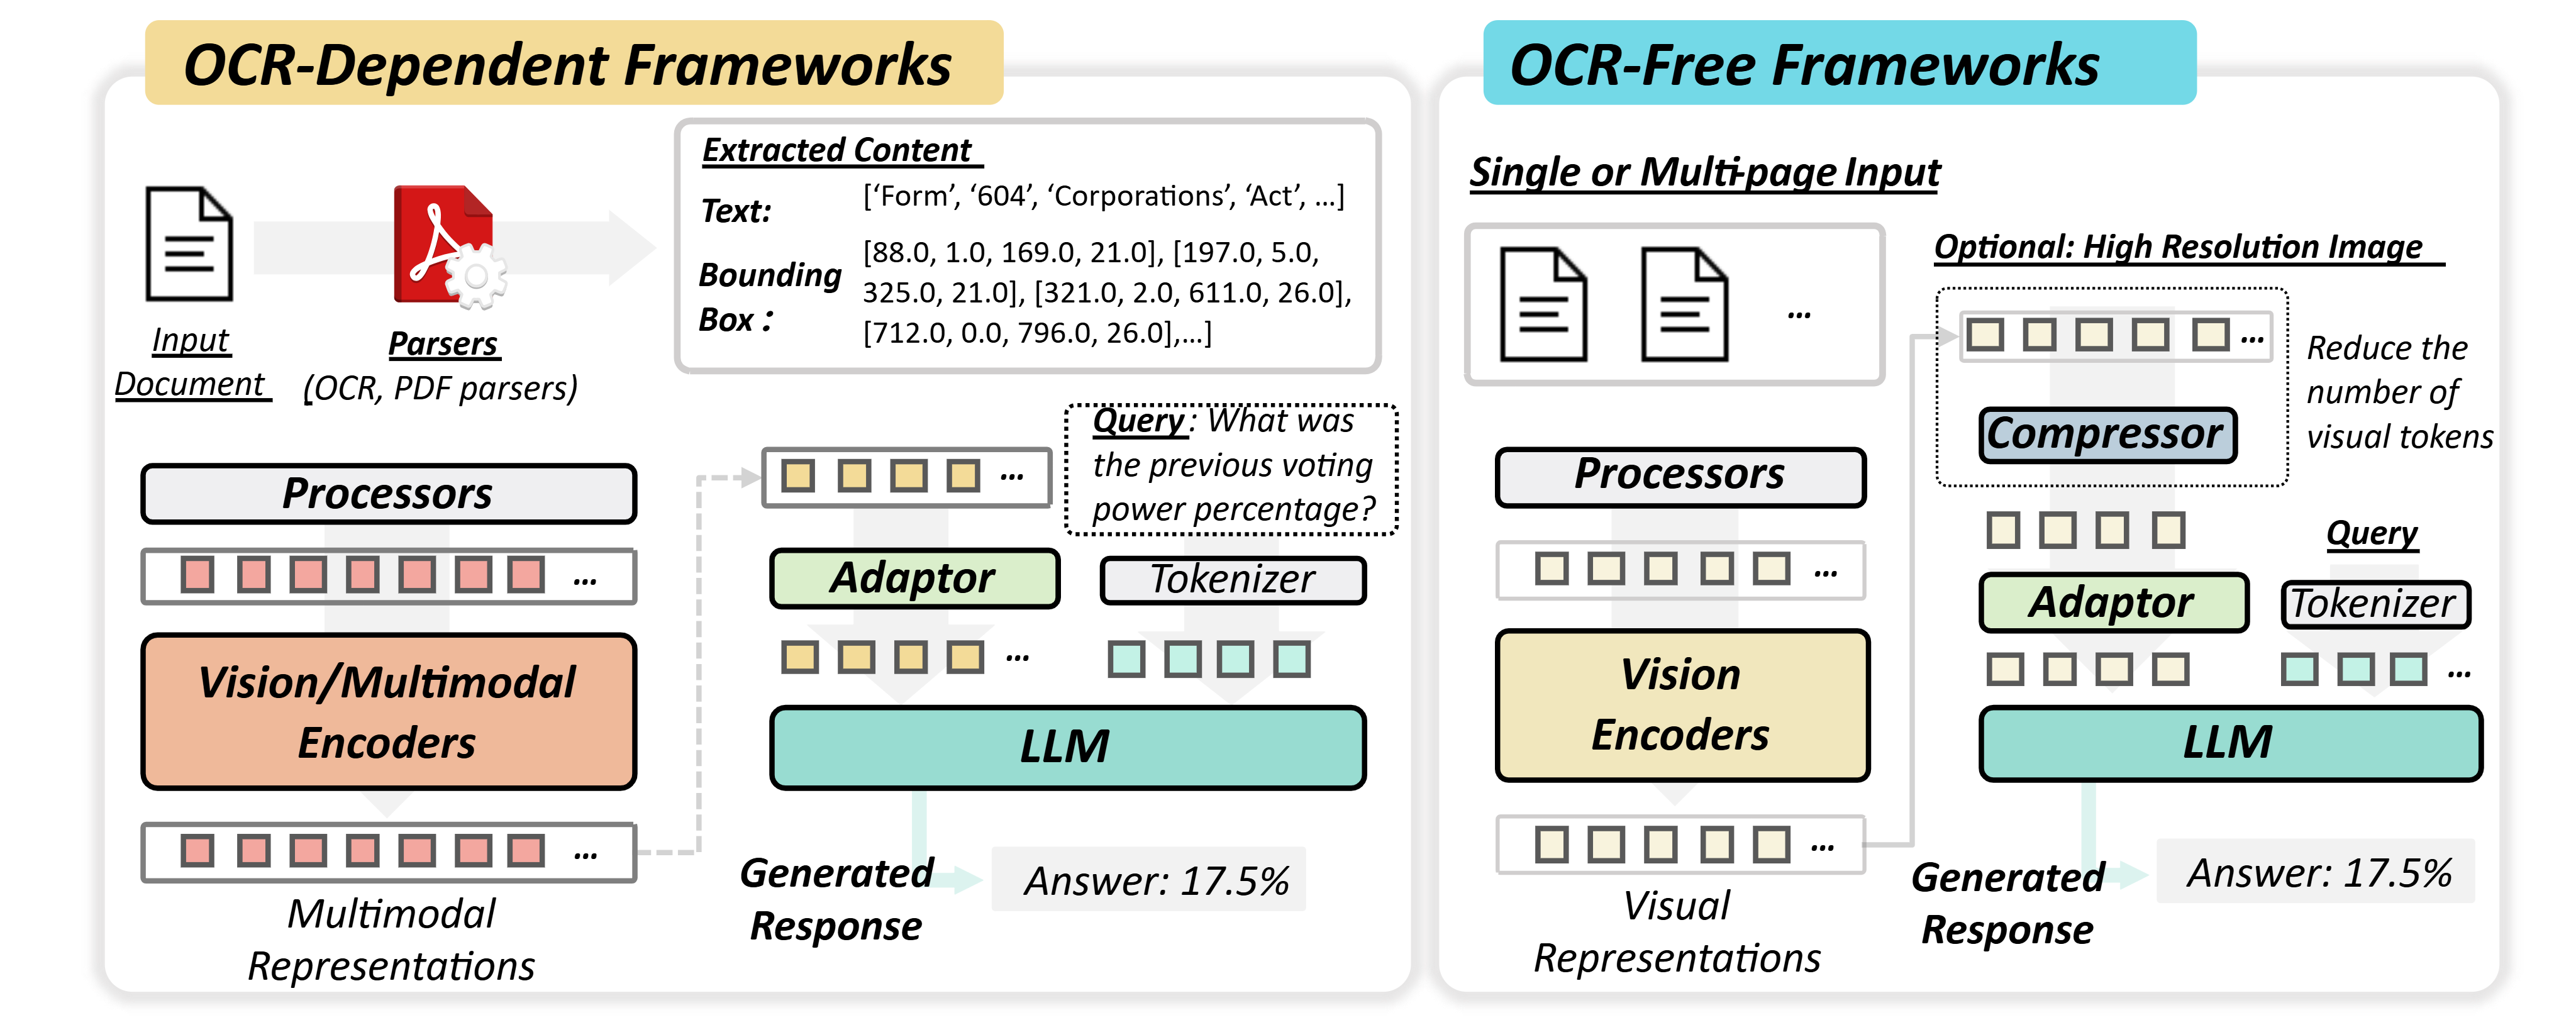
\includegraphics[width=0.9\columnwidth]{include/sp_architectures.png}
    \caption{OCR-dependent and OCR-free framework architectures for MLLM-based VRDU. Adapted from Ding et al. \citep{ding2026survey}.}
    \label{fig:sp_architectures}
\end{figure}

\paragraph{MLLM-based VRDU Architectures.} At the architectural level, single-page systems divide into two families, shown in Figure~\ref{fig:sp_architectures}. OCR-dependent frameworks parse the page first, running off-the-shelf OCR or a PDF parser to recover text alongside its bounding-box coordinates. These parsed signals are then encoded, either injected as text into the language model prompt \citep{wang2024docllm} or passed through a vision or multimodal encoder such as LayoutLMv3 that binds text, layout, and image into joint multimodal representations \citep{huang2022layoutlmv3, luo2024layoutllm}, which an adaptor and tokeniser convert into the token sequence the language model consumes. Relying on the parser lets these systems capture structural information without heavy visual pretraining, but ties their accuracy to the parser's, most visibly on handwritten or low-quality scans where recognition degrades. OCR-free frameworks discard the parser and let a vision encoder read the rendered page directly from pixels, producing visual representations that the language model is trained to interpret through objectives such as text recognition and grounding \citep{hu2024mplug, wang2023towards}. Because fine-grained text is legible only at high resolution, these frameworks consume large images and often insert a compression step to reduce the resulting visual token count before the language model \citep{hu2025mplug}; in exchange, they train end to end and handle handwriting and irregular layouts that OCR struggles with.

\begin{figure}[ht]
    \centering
    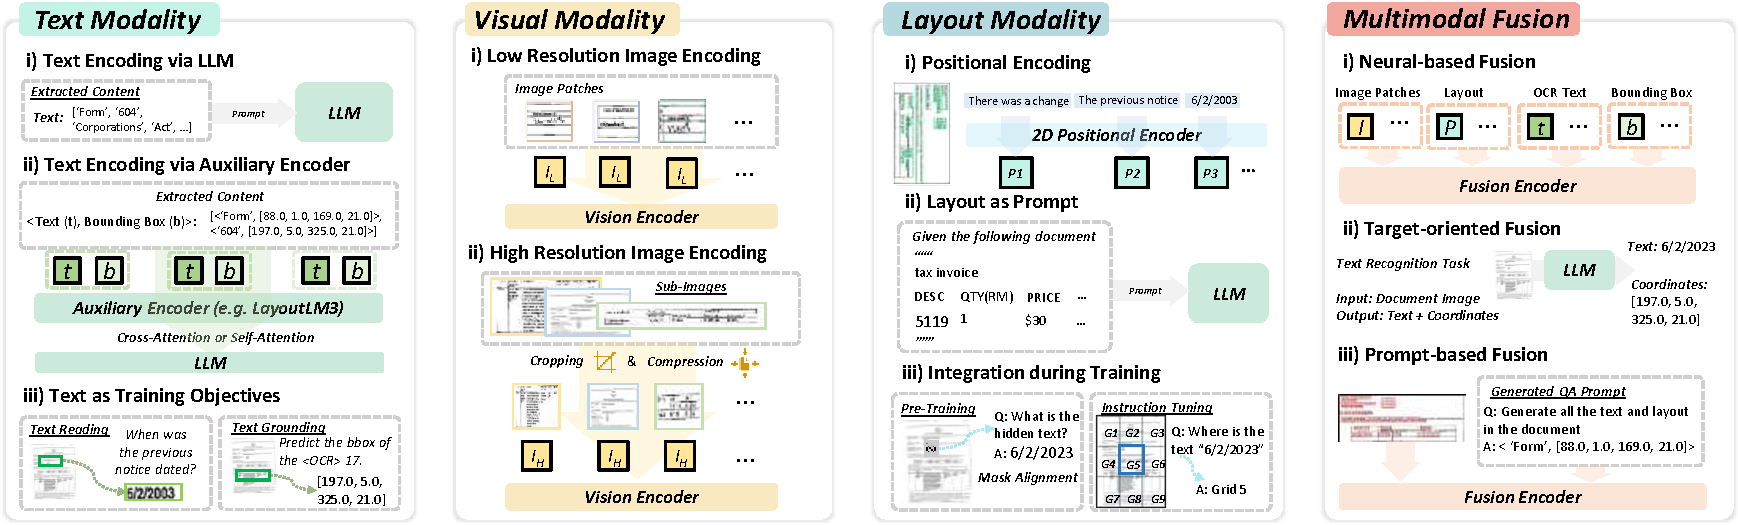
\includegraphics[width=\columnwidth]{include/sp_modalities.pdf}
    \caption{Multimodal feature representation and fusion mechanisms. Adapted from Ding et al. \citep{ding2026survey}.}
    \label{fig:sp_modalities}
\end{figure}

\paragraph{Single-page Multimodal Representation.} Within both families, a system must still decide how to represent text, layout, and visual content, and how to fuse them (Figure~\ref{fig:sp_modalities}). Text is recovered as injected OCR strings \citep{wang2024docllm}, through joint text-layout-vision encoders \citep{luo2024layoutllm, zhu2025enhancing}, or as a pretraining objective for the vision encoder itself \citep{wang2025marten}. Layout is encoded as positional features attached to text tokens \citep{xu2020layoutlm, zhu2025enhancing}, as coordinates verbalised in the prompt \citep{perot2024lmdx}, or through dedicated layout tokens \citep{zhu2025simple}. Visual content is managed through low-resolution patch embeddings \citep{tanaka2024instructdoc}, high-resolution shape-adaptive cropping \citep{ye2023ureader, hu2024mplug}, or token compression that cuts the visual sequence by an order of magnitude \citep{hu2025mplug, yu2024texthawk2}. Fusion draws these together through dedicated multimodal encoders \citep{huang2022layoutlmv3}, shared training objectives \citep{hu2024mplug, wang2025marten}, or prompt-based interleaving of text, layout, and images. Single-page systems make these choices assuming the entire document fits in a single backbone input; the multi-page setting (Chapter~\ref{ch:survey}), breaks that assumption, reframing each choice around which pages or regions the system should attend to in the first place.

% \subsection{Challenges of the Multi-Page Setting}
% \label{sec:bg-challenges}
% Answering a question over a long multi-page document usually requires only a small fraction of the document content, though some tasks, such as whole-document summarisation, draw on the whole document. Feeding the entire document to an MLLM is not a general solution, since long multi-page documents routinely exceed what a backbone can hold in its context window~\cite{xu2026managing}. MP-VRDU systems must therefore select which parts of the document reach the MLLM backbone. Scaling MLLMs to longer contexts does not resolve this: long-context models attend poorly to evidence buried mid-input \citep{liu2024lost}, and the memory and compute required grow with sequence length, so the achievable context is bounded by the capacity of current hardware rather than by the architecture alone. Answering often requires integrating evidence from several parts of a document at once, so a system must locate every relevant evidence unit rather than the single best one, and missing any of them is enough to answer incorrectly or be unable answer at all \citep{xu2026locating}. Compounding the challenge, cross-page structure such as section hierarchy and cross-references cannot be recovered from any part of the document in isolation \citep{tito2023hierarchical}, and questions often require such cross-page structural to formulate to gather evidence for the correct answer.


% ============================================================================
%  Survey
% ============================================================================
\chapter{Survey of Architectures and Techniques}
\label{ch:survey}

This chapter is adapted from \textbf{Managing Evidence at Document Scale: A Survey of Multi-Page Visually Rich Document Understanding}~\cite{xu2026managing}, by \textbf{Lewei Xu}, Yihao Ding, Zihan Xu, Siwen Luo, Daochang Liu, and Wei Liu, published in the \emph{Main Conference of EMNLP 2026}. The first author was responsible for constructing the surveyed literature corpus, including paper identification and selection; developing the architectural taxonomy used to organise MP-VRDU systems; and preparing the technical content, including the survey analysis, appendix material, and tables. \textbf{This chapter additionally serves as the Literature Review of this thesis.}

\section{Introduction}
\label{section:survey_intro}
MP-VRDU has seen rapid growth in recent years, with new architectures, training strategies, and inference methods emerging. Existing work has explored joint multi-page encoding \citep{tito2023hierarchical}, adaptation of pretrained MLLMs \citep{duan2025docopilot}, retrieval-augmented pipelines that decouple evidence selection from generation \citep{cho2024m3docrag}, and adaptive controllers that gather evidence iteratively at inference time \citep{sun2025docagent}, often combined with task-specific training or prompted reasoning loops \citep{xiong2026docr1, han2025mdocagent}. However, this body of work has developed along largely parallel lines, with limited cross-family comparison and inconsistent terminology, and few works explicitly distinguish what is genuinely multi-page-distinctive from what is inherited from the single-page setting. As a result, the field lacks a unified view of the design choices that matter most in multi-page settings, motivating the systematic organisation this chapter provides.

Prior surveys have charted VRDU from complementary angles. Subramani et al.~\citep{subramani2020survey} survey the OCR-centric deep-learning pipelines of the pre-MLLM era, covering text detection, recognition, and layout analysis as separate stages. Ding et al.~\citep{ding2026deep} and Gbada et al.~\citep{gbada2025deep} both treat information extraction over visually rich documents, while a more recent survey by Ding et al.~\citep{ding2026survey} covers the shift to MLLM-based architectures, training strategies, and benchmarks. Closest to the multi-page setting, Gao et al.~\citep{gao2026scaling} survey multimodal retrieval-augmented generation as a means of scaling document understanding to the multi-page setting. Several of these include multi-page systems among the work they cover, but none treats multi-page understanding as a distinct problem with its own design axes, addressing it only in passing within a broader single-page or extraction-focused scope.
\footnote{A detailed survey comparison table is provided in Appendix~\ref{app:survey-comparison}.}

\textbf{Our contributions are as follows}: \textbf{(1)} We define MP-VRDU as a distinct document-understanding problem and organise the field through an evidence-management perspective. \textbf{(2)} We introduce a new architectural taxonomy for MP-VRDU, grouping existing systems into four families according to how they manage document-scale evidence (\S\ref{sec:architecture}). \textbf{(3)} We provide a systematic survey of the architectures, multimodal representations, inference-time and training strategies, datasets, and evaluation practices used in MP-VRDU (\S\ref{sec:modality}-\S\ref{sec:datasets}). \textbf{(4)} We identify the principal open challenges that define the current frontier of the field with broader implications and future directions (deferred to Chapter~\ref{ch:conclusion}).

% ─────────────────────────────────────────────────────────────────────────────
% Auto-generated by summary_models_convert.py — do NOT edit manually.
% Re-generate:  python3 summary_models_convert.py models_summary.csv models_summary.tex
%
% Required packages (add to your preamble):
%   \usepackage{booktabs}
%   \usepackage{longtable}
%   \usepackage{array}
%   \usepackage{xcolor}
%   \usepackage{colortbl}
%   \usepackage{caption}
%   \usepackage{adjustbox}   % for \begin{adjustbox}
%   \usepackage{natbib}      % for \citeyear  (or use biblatex)
%   \usepackage{lscape}      % optional: landscape
% ─────────────────────────────────────────────────────────────────────────────

\definecolor{sectionbg}{gray}{0.88}

% ── tab:model_survey_arch ──────────────────────────────────────────────────────────────
\begin{table*}[!t]
\centering
% \small
\scriptsize
\captionsetup{font=small}
\setlength{\tabcolsep}{3pt}
\renewcommand{\arraystretch}{0.86}
\begin{adjustbox}{width=\textwidth}
\begin{tabular}{l l c l l c c c c}
\toprule
\textbf{Model} & \textbf{Venue} & \textbf{OCR} & \textbf{Vision Encoder} & \textbf{LLM Backbone} & \textbf{Mod.} & \textbf{Search} & \textbf{Reasoning} & \textbf{Agentic} \\
\midrule

% ── Page-to-Document Encoding Models ─────────────────────────────────────────────────────────────
\rowcolor{sectionbg}
\multicolumn{9}{l}{\textbf{Page-to-Document Encoding Models}} \\
\midrule
  {Arctic-TILT}~(\citeyear{borchmann2025arctic}) & ACL & Yes & U-Net & T5-Large & T, V, L & - & - & - \\
  {GRAM}~(\citeyear{blau2024gram}) & CVPR & Yes & DocFormerv2 & DocFormerv2 & T, V, L & - & - & - \\
  {Hi-VT5}~(\citeyear{tito2023hierarchical}) & PR & Yes & DiT & T5-Base & T, V, L & - & - & - \\
  {RM-T5}~(\citeyear{dong2024multi}) & DAS & Yes & DiT & T5-Base & T, V, L & - & - & - \\

\midrule[0.4pt]

% ── MLLM-Centric Adaptation Models ─────────────────────────────────────────────────────────────
\rowcolor{sectionbg}
\multicolumn{9}{l}{\textbf{MLLM-Centric Adaptation Models}} \\
\midrule
  {DocR1}~(\citeyear{xiong2026docr1}) & AAAI & No & Qwen2.5-VL & Qwen2.5-VL-7B & V & - & CoT, HD & - \\
  {DocSeeker}~(\citeyear{yan2026docseeker}) & CVPR & No & Qwen2.5-VL ViT & Qwen2.5-VL-7B & V & - & CoT, HD & - \\
  {Leopard}~(\citeyear{jia2025leopard}) & TMLR & No & SigLIP-SO400M & Mult. (La/Mi) & V & - & CoT & - \\
  {mPLUG-DocOwl2}~(\citeyear{hu2025mplug}) & ACL & No & ViT-L/14 & mPLUG-Owl2 & V & - & - & - \\
  {URaG}~(\citeyear{shi2026urag}) & AAAI & No & Qwen2.5-VL ViT & Qwen2.5-VL-3B/7B & V & - & HD & - \\
  {Docopilot}~(\citeyear{duan2025docopilot}) & CVPR & No* & InternViT-300M & Mult. (In) & V & - & - & - \\
  {Texthawk2}~(\citeyear{yu2024texthawk2}) & preprint & No* & SigLIP-SO400M & Qwen2-7B & V & - & - & - \\
  {DocSLM}~(\citeyear{hannan2026docslm}) & CVPR & Yes & SigLIP2 & Qwen2.5-1.5B & T, V, L & - & - & - \\
  {InstructDoc}~(\citeyear{tanaka2024instructdoc}) & AAAI & Yes & CLIP & FlanT5, BLIP2 & T, V, L & - & - & - \\
  {LayTokenLLM}~(\citeyear{zhu2025simple}) & CVPR & Yes & - & Mult. (La/Qw) & T, L & - & - & - \\
  {CoR}~(\citeyear{guo2026end}) & preprint & Yes* & Qwen2.5-VL & Qwen2.5-VL-7B & T, V & - & CoT, PE, HD & - \\

\midrule[0.4pt]

% ── Retrieval-Augmented Pipelines ─────────────────────────────────────────────────────────────
\rowcolor{sectionbg}
\multicolumn{9}{l}{\textbf{Retrieval-Augmented Pipelines}} \\
\midrule
  {AVIR}~(\citeyear{li2026avir}) & MMAsia & No & Pix2Struct & Qwen2.5-VL-3B & V & D & - & - \\
  {DFVC}~(\citeyear{qian2026accurate}) & MDPI & No & VisRAG, ColQwen & Qwen2-VL-2B & V & D & - & - \\
  {DREAM}~(\citeyear{zhang2025dream}) & MM & No & InternVL2 ViT & InternVL2-4B & V & J & HD & - \\
  {M3DocRAG}~(\citeyear{cho2024m3docrag}) & preprint & No & ColPali, ColQwen & Mult. (Qw/In/Id) & V & D & - & - \\
  {MM-R5}~(\citeyear{xu2025mm}) & AAAI & No & Qwen2.5-VL ViT & Qwen2.5-VL-7B & V & D & CoT & - \\
  {MoLoRAG}~(\citeyear{wu2025molorag}) & EMNLP & No & ColPali & Mult. (Qw/DS/Lv) & V & D, Nav & - & 1A \\
  {Self-Attention Scoring}~(\citeyear{kang2024multi}) & ICDAR & No & Pix2Struct & Pix2Struct & V & D & - & - \\
  {SLEUTH}~(\citeyear{liu2025resolving}) & CVPR & No & ColPali, Qwen3-VL ViT & Mult. (Qw/GL/Ge) & V & D & HD & 4A \\
  {SV-RAG}~(\citeyear{chen2025sv}) & ICLR & No & InternVL2, Phi-3-vision & Mult. (In/Pa/Ph) & V & D & - & - \\
  {VDocRAG}~(\citeyear{tanaka2025vdocrag}) & CVPR & No* & Phi3V-4.2B & Phi3V-4.2B & V & D & - & - \\
  {CREAM}~(\citeyear{zhang2024cream}) & ACM & Yes & Pix2Struct & LLaMA2-7B & T, V & J & HD & - \\
  {KGP}~(\citeyear{wang2024knowledge}) & AAAI & Yes & - & Mult. & T, L & S, IR, Nav & - & 1A \\
  {MHier-RAG}~(\citeyear{gong2026mhier}) & preprint & Yes & Qwen-VL-Plus & Mult. (Qw/DS/GPT) & T, V, L & J & CoT, HD & - \\
  {MLDocRAG}~(\citeyear{zhang2026mldocrag}) & preprint & Yes & Qwen2.5-VL & Mult. (Qw) & T, V, L & D & CoT, HD & - \\
  {MultiDocFusion}~(\citeyear{shin2026multidocfusion}) & ACL & Yes & - & Mult. (Qw/La/Mi) & T, V, L & D & HD & - \\
  {M2RAG}~(\citeyear{duan2025m2rag}) & NeurIPS & Yes* & VisRAG-Ret & Mult. (Qw) & T, V & J & - & 3A \\
  {MDocAgent}~(\citeyear{han2025mdocagent}) & preprint & Yes* & ColPali, ColQwen2 & Mult. (La/Qw) & T, V & J & - & 5A \\
  {PDF-WuKong}~(\citeyear{xie2026pdf}) & IJCV & Yes* & IXC2-VL-4KHD & IXC2-VL-4KHD & T, V & J & - & - \\
  {RAG-DocVQA}~(\citeyear{pez2025enhancing}) & ICDAR & Yes* & DiT, Pix2Struct & Qwen2.5-VL-7B & T, V, L & D & - & - \\
  {VisDoMRAG}~(\citeyear{suri2025visdom}) & NAACL & Yes* & ColPali / ColQwen2 & Mult. (Qw/Ge/GPT) & T, V & J & CoT & 3A, SC \\

\midrule[0.4pt]

% ── Adaptive-Trajectory Pipelines ─────────────────────────────────────────────────────────────
\rowcolor{sectionbg}
\multicolumn{9}{l}{\textbf{Adaptive-Trajectory Pipelines}} \\
\midrule
  {Doc-V*}~(\citeyear{zheng2026doc}) & ACL & No & Qwen2.5-VL & Qwen2.5-VL-7B & V & D, IR, QR, Nav & ReAct, HD & 1A \\
  {DocReact}~(\citeyear{wu2025doc}) & ACL & No & ColPali, VisRAG & GPT-4o & V & D, IR, QR & ReAct, QD & 1A \\
  {MACT}~(\citeyear{yu2025visual}) & preprint & No & Multiple & Mult. (Qw/MM/In) & V & D & CoT, PE & 4A, SC, SV \\
  {VRAG-RL}~(\citeyear{wang2025vrag}) & NeurIPS & No & Qwen2.5-VL ViT & Qwen2.5-VL-3B/7B & V & D, IR, QR & ReAct, HD & 1A \\
  {DocLens}~(\citeyear{zhu2026doclens}) & ACL & Yes & -- & Mult. (GPT/Ge/Cl) & T, V, L & J & CoT & 4A, SA \\
  {DMAP}~(\citeyear{fu2026dmap}) & WWW & Yes* & ColPali & Mult. (GPT/Qw) & T, V, L & J & HD & 2A, SR \\
  {DocAgent}~(\citeyear{sun2025docagent}) & EMNLP & Yes* & -- & Mult. (GPT/Ge/Cl) & T, V, L & J, IR, Nav & ReAct, HD & 3A \\
  {DocDancer}~(\citeyear{zhang2026docdancer}) & preprint & Yes* & Qwen3-VL-235B & Qwen3-4B/30B & T, V, L & J, IR, QR & ReAct & 1A \\
  {MM-Doc-R1}~(\citeyear{lin2026mm}) & ACL & Yes* & Qwen2.5-VL ViT & Qwen3-4B/8B & T, V & S, IR, QR, Nav & ReAct, HD & 3A \\
  {SimpleDoc}~(\citeyear{jain2025simpledoc}) & EMNLP & Yes* & ColQwen-2.5 & Mult. (Qw) & T, V & J, IR, QR & - & 1A, SR, SV \\
  {ViDoRAG}~(\citeyear{wang2025vidorag}) & EMNLP & Yes* & NV-Embed-V2, ColQwen2 & Mult. (Qw/La/GPT) & T, V & J, IR & ReAct, HD & 3A, SR, SV \\

\bottomrule
\end{tabular}
\end{adjustbox}
\caption{Survey of MP-VRDU models grouped by architecture. T\,=\,text; V\,=\,visual; L\,=\,layout. CoT\,=\,Chain of Thought; ReAct\,=\,Reason\,+\,Act; PE\,=\,Plan-Execute; QD\,=\,Question Decomposition; HD\,=\,Hierarchical / Coarse-to-Fine. S\,=\,Sparse; D\,=\,Dense; J\,=\,Joint; IR\,=\,Iterative Retrieval; QR\,=\,Query Reformulation; Nav\,=\,Navigation. $n$A\,=\,$n$ agents; SR\,=\,Self-Refine; SV\,=\,Self-Verify; SC\,=\,Self-Consistency; SA\,=\,Sampling-Adjudication. OCR column: Yes$^*$\,=\,not OCR-dependent; No$^*$\,=\,OCR-derived supervision explicitly used during training. \textit{Mult.} denotes a system evaluated on multiple backbones: Qw\,=\,Qwen; Ge\,=\,Gemini; GL\,=\,GLM; Cl\,=\,Claude; DS\,=\,DeepSeek; In\,=\,InternVL; Id\,=\,Idefics; La\,=\,LLaMA; Lv\,=\,LLaVA; Mi\,=\,Mistral; MM\,=\,MiMo; Ph\,=\,Phi; Pa\,=\,PaliGemma. `--' indicates not reported.}
\label{tab:model_survey_arch}
\end{table*}

\section{Methodology and Scope}
\label{sec:methodology}
This chapter covers MP-VRDU systems published from 2023 (starting from MP-DocVQA's Hi-VT5~\cite{tito2023hierarchical}) across major venues such as CVPR, ACL, EMNLP, and ICLR. Candidates were identified through keyword search over multi-page terms (``long document'', ``cross-page reasoning'', ``page-level retrieval'') combined with task and method terms (``document visual question answering'', ``document RAG'', ``long-context vision-language model''), supplemented by forward-citation sweeps anchored on established benchmarks such as MP-DocVQA, MMLongBench-Doc, and LongDocURL. We then manually screened for substantive multi-page contributions such as novel architectures, retrieval mechanisms, or training strategies. The dataset catalogue covers datasets used by the surveyed systems, plus a small number of relevant but underused ones. Rather than a systematic scoping review aiming at exhaustive retrieval, we prioritise representative coverage of the design space, since MP-VRDU is evolving rapidly and its terminology remains in flux. Full surveyed corpus details, search terms and inclusion criteria are available in Appendix~\ref{app:sv_methodology}.

\section{Multi-Page Architectural Overview}
\label{sec:architecture}
The defining problem in MP-VRDU is evidence management, and how a system manages cross-page evidence is fixed by its architectural design, which determines \textbf{how evidence is selected, preserved, and exposed for reasoning}. We therefore organise the field by architecture rather than by the OCR dependency used in prior surveys~\citep{ding2026survey}, into four families.
\textit{Page-to-document encoding models} jointly encode pages with cross-page representations (\S\ref{sec:arch-p2d}).
\textit{MLLM-centric adaptation models} adapt MLLMs to multi-page inputs within context and token budgets (\S\ref{sec:arch-mllm}).
\textit{Retrieval-augmented pipelines} retrieve relevant evidence before generation (\S\ref{sec:arch-ra}).
\textit{Adaptive-trajectory pipelines} iteratively inspect evidence using an LLM controller (\S\ref{sec:arch-agent}). Reported performance across the four families on principal MP-VRDU benchmarks is provided in Appendix~\ref{app:performance} (Table~\ref{tab:model_performance_arch}).

\begin{figure}[h]
    \centering
    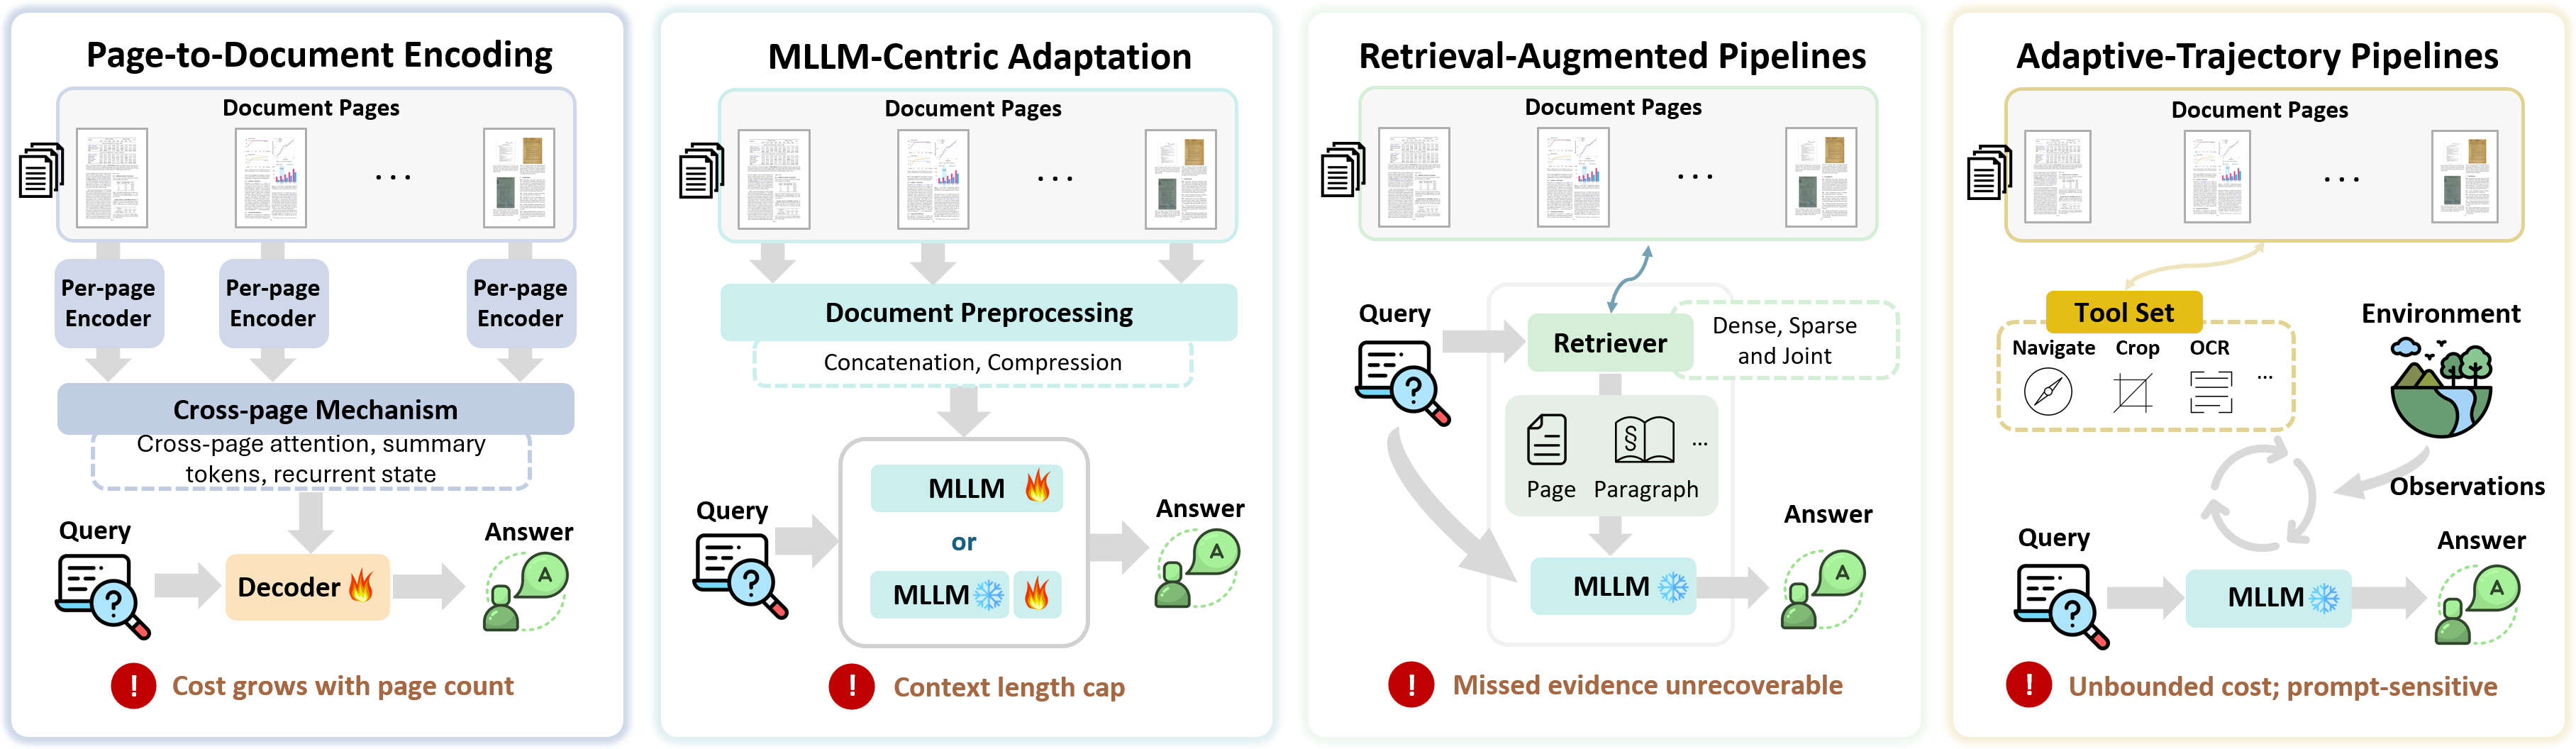
\includegraphics[width=\columnwidth]{survey/figures/models_arch.png}
    \caption{Illustration of MP-VRDU Architectures. Snowflake indicates typically frozen; Fire indicates typically trained; Both indicates even split.}
    \label{fig:models_arch}
\end{figure}

\subsection{Page-to-Document Encoding Models} 
\label{sec:arch-p2d}

Page-to-document encoding models process each page through a shared layout-aware document encoder such as LayoutLMv3~\cite{huang2022layoutlmv3} that fuses OCR text, layout, and visual features at the page level, then connect per-page representations through a document-level exchange mechanism within a single forward pass. The mechanism may take the form of per-page summary tokens~\cite{tito2023hierarchical}, document-global tokens with local-global attention~\cite{blau2024gram}, recurrent memory states passed across pages~\cite{dong2024multi}, or sparse cross-page attention over long OCR sequences~\cite{borchmann2025arctic}. By preserving page identity, local layout, and reading order in the architecture itself, this design provides a strong inductive bias for multi-page structure and is well suited to documents with regular templates such as multi-page forms and business reports~\cite{tito2023hierarchical, borchmann2025arctic}. The principal limitation is intrinsic to the design: every page is still encoded jointly in a single forward pass, and the per-page compression step that enables document-level exchange discards fine-grained evidence as inputs scale. As the context windows of pretrained MLLMs have widened, the motivation for a dedicated cross-page encoder has weakened, and subsequent families absorb cross-page information into the backbone or select evidence before reading.

\subsection{MLLM-Centric Adaptation Models}
\label{sec:arch-mllm}

MLLM-centric adaptation models remove the dedicated cross-page encoder entirely and process the document inside a pretrained MLLM backbone whose context window absorbs cross-page information directly, with adaptation ranging from training only lightweight modules to fine-tuning the backbone itself. At the lightweight end, \emph{projectors} that map per-modality features into the backbone's token space~\cite{tanaka2024instructdoc} and \emph{adapters} that insert small trainable modules into a frozen backbone for parameter-efficient fine-tuning~\cite{zhu2025simple} keep most weights fixed, while visual-token compression further constrains token growth on long inputs to keep multi-page documents within the context budget~\cite{hu2025mplug}. At the heavier end, the MLLM backbone itself is unfrozen for continued pretraining or instruction tuning on document corpora, trading parameter efficiency for stronger document-specific grounding~\cite{duan2025docopilot}, with long-context tuning further improving performance on documents of moderate length~\cite{hu2024mplug, yu2024texthawk2}. The family inherits the foundation MLLM's instruction-following and reasoning, avoids the engineering overhead of external retrieval or orchestration, and remains parameter-efficient to train. The cost of this design is that performance degrades on longer documents~\cite{jia2025leopard}: as most models in this category are OCR-free, reliable text recovery depends on high-resolution input that aggressive token compression readily compromises, and document structure such as section hierarchy and figure-caption linkage must be recovered implicitly from pixels rather than supplied through dedicated tokens~\cite{hannan2026docslm, duan2025docopilot}. Combined with the attention-dilution problem~\cite{liu2024lost}, these limitations motivate subsequent families that move evidence selection out of the backbone altogether.

\subsection{Retrieval-Augmented Pipelines} 
\label{sec:arch-ra}

Retrieval-augmented pipelines decouple evidence selection from answer generation: a retriever first selects relevant evidence units, such as textual chunks, pages, or graph nodes, and the generator then produces an answer conditioned on this compact subset~\cite{cho2024m3docrag, tanaka2025vdocrag}. This separation allows the pipeline to scale to multi-page inputs that exceed what MLLM-centric and page-to-document encoding models can hold in a single context, since inference cost depends on the retrieved content rather than on document length. The retriever may be a sparse lexical scorer, a dense embedding model, or a structure-aware index over a parsed representation of the document (\S\ref{sec:tf-retrieval}), and the generator is typically a pretrained MLLM. The family spans single-pass retriever-generator systems~\cite{cho2024m3docrag} to multi-component pipelines that compose multiple LLM-instantiated ``agents'' in specialised roles such as modality-specific reading branches~\cite{han2025mdocagent} or modality-fusion synthesis~\cite{duan2025m2rag}, but in either case the control flow is set at design time. Modular decomposition lets the retriever and generator be swapped independently, the retrieved evidence provides a partial audit trail for the answer, and the same interface extends to multi-document corpora without architectural change. Because the flow is fixed, evidence missed or poorly ranked at retrieval is unrecoverable at generation, questions that require aggregating multiple weakly relevant pages frequently fail~\cite{wu2025molorag}, and upstream errors in chunking, OCR, or modality alignment propagate directly into the answer.

\subsection{Adaptive-Trajectory Pipelines} 
\label{sec:arch-agent}

Adaptive-trajectory pipelines instantiate the agent paradigm characterised by \citet{plaat2025agentic} and \citet{wang2024survey}, in which one or more LLM controllers reason, act on an external environment, and condition each subsequent action on observed outcomes rather than executing a plan fixed in advance~\cite{zheng2026doc, sun2025docagent}. Unlike the fixed-role agents of \S\ref{sec:arch-ra}, the controller's trajectory is not predetermined: it selects each evidence-gathering action at inference time, with actions surfacing as explicit calls to external retrievers, parsers, or OCR engines~\cite{wang2025vidorag, yu2025visual}, or as structured responses the framework interprets as a re-retrieval or as navigation over a pre-built document representation~\cite{jain2025simpledoc}. A controller might issue a refined query when the first retrieval returned irrelevant pages, request a higher-resolution view of a page surfaced by an earlier pass, or follow a cross-reference from one section to another. ReAct~\cite{yao2023react} is the most common controller realisation (\S\ref{sec:tf-reasoning}), though other variants also appear. Because the trajectory is constructed rather than fixed, compute scales with question difficulty rather than document length, and the full action sequence becomes an inspectable audit trail. The cost of that flexibility is that inference cost is difficult to bound in advance, controllers are sensitive to prompt phrasing and may commit early to wrong evidence and continue confidently down the wrong trajectory without surfacing the error, stochastic generation complicates reproducibility, and the system still inherits the recall ceiling of every retriever, parser, or scoring module it consults.

\section{MP-VRDU Multimodal Representation}
\label{sec:modality}

Every evidence-management decision is enacted over a specific modality, and its cost depends on how that modality is represented. While Section~\ref{sec:architecture} categorises MP-VRDU systems by where cross-page evidence is processed, this section analyses the problem from a modality perspective. MP-VRDU systems must locate sparse evidence across long multimodal contexts, forcing each modality to trade \emph{page coverage} (how much of the document the system can attend to) against \emph{reading fidelity} (how accurately each attended region is interpreted), since long-context models attend poorly to evidence buried in the middle of long inputs~\cite{liu2024lost}. The single-page mechanisms inherited from prior work, including OCR-text injection, per-image patch encoding, and per-token layout signals, are reviewed in Section~\ref{sec:bg-sp}; here we concentrate on the multi-page pressures that text (\S\ref{sec:modality-text}), visual (\S\ref{sec:modality-visual}), and cross-page structural (\S\ref{sec:modality-structure}) evidence introduce.

\subsection{Text Modality}
\label{sec:modality-text}
Text in MP-VRDU presents four bottlenecks. \textbf{Volume} across pages routinely exceeds what the MLLM can process in full. This is addressed either by compressing all pages into a fixed budget through page summaries, memory tokens, or long-context encoders~\cite{borchmann2025arctic, dong2024multi, hu2025mplug}, or by indexing chunks and passing only selected text to the reader~\cite{xie2026pdf, zhang2024cream, cho2024m3docrag}. The first approach fixes compression before the question is seen, so evidence absent from the compressed representation cannot be recovered later in the pipeline; the second makes evidence missed at retrieval unrecoverable at the reading stage, and broadening the retrieved set merely shifts the cost from omission to a related failure mode known as \emph{attention dilution}, in which the model spreads its attention across too many candidate passages and loses focus on the answer-bearing ones~\cite{liu2024lost}. \textbf{Continuity} breaks when paragraphs, tables, and section context span page boundaries. This is preserved by recurrent state propagation that carries page context forward across the document~\cite{dong2024multi}, structure-aware chunking that groups text under recovered section headings rather than along sliding-window boundaries~\cite{shin2026multidocfusion}, and adjacent-page expansion at retrieval time that pulls in neighbouring pages when a candidate is surfaced~\cite{qian2026accurate}. Each restores local cross-page context at the cost of broader query relevance, since the additional context is selected by proximity rather than by question. \textbf{Noise} accumulates as OCR and parsing errors compound across pages: a recognition error rate that is tolerable on a single page multiplies over a long document, and because extracted text is the retrieval index in most pipelines, these errors degrade retrieval as well as reading, surfacing wrong pages or burying the right ones. It is dampened upstream through layout-aware parsing pipelines that reduce recognition error, or downstream by treating low-confidence tokens as soft cues the reader can discount rather than as ground truth~\cite{hannan2026docslm}, yet how noise propagates through multi-page retrieval indexes remains largely uncharacterised. \textbf{Heterogeneity} in text density varies sharply across pages within a single document, yet receives the least attention: most systems apply fixed token budgets and fixed top-$k$ uniformly across pages and queries, over-compressing dense pages while wasting capacity on sparse ones. Adaptive selection that scales the returned set with the per-query score distribution~\cite{li2026avir} only begins to address this variability, and no current system varies its per-page text budget within a single document.

\subsection{Visual Modality}
\label{sec:modality-visual}
Visual evidence preserves signals that text extraction loses, but its cost structure introduces three bottlenecks of its own. \textbf{Resolution} cannot be maintained at full document length, since token cost scales with page count multiplied by per-page resolution, forcing a choice between compression and selective high-fidelity reading. Token-reduction modules and adaptive sub-image budgets~\cite{hu2025mplug, yu2024texthawk2, jia2025leopard} keep every page available in context but leave fine-grained content, including small text, table cells, and chart annotations, vulnerable to downsampling. Inspecting only a retrieved subset at high resolution~\cite{zhu2026doclens, jain2025simpledoc} preserves detail at the cost of inheriting the selector's recall ceiling: pages not surfaced by the retriever are never read, regardless of the relevance of their content. \textbf{Multi-signal competition} arises because the same visual budget must support text-bearing pixels, non-textual evidence such as charts, figures, and handwriting, and layout cues within a single page. Visual RAG systems, which retrieve over rendered page images rather than over extracted text, encode pages directly so all signals share one representation~\cite{cho2024m3docrag, tanaka2025vdocrag}; the page becomes a single evidence unit that cannot be decomposed at retrieval time. Element-level cropping of tables, figures, and charts~\cite{zhu2026doclens} preserves fine structure at the cost of detector dependence and separation from the surrounding explanatory text on which interpretation often depends. A third route delegates text recovery to an OCR pipeline so the visual budget can prioritise non-textual evidence~\cite{hannan2026docslm}, which avoids the budget competition at the cost of inheriting OCR fragility on handwriting and complex layouts. \textbf{Heterogeneity} in visual complexity varies sharply across pages within a single document, yet receives the least attention: most systems apply uniform resolution and sub-image budgets regardless of whether a page is a sparse cover sheet or a dense table-laden appendix, and evidence-guided allocation that varies the visual budget by content~\cite{yan2026docseeker} only begins to address per-page and per-query variability.

\subsection{Cross-Page Structure Modality}
\label{sec:modality-structure}
Structure turns isolated page observations into document evidence. Per-token layout remains relevant at the multi-page scale, with specialised tokens encoding spatial geometry within each page~\cite{zhu2025simple}, but the MP-distinctive difficulty is relationships whose scope crosses pages. \textbf{Hierarchy and reading order} is the foundational problem: sections, lists, columns, and captions routinely span page boundaries, and the same evidence may serve different reasoning paths depending on which parent section it sits under. Explicit parsers expose this structure as outlines, trees, or hierarchical indices that retrieval can navigate~\cite{shin2026multidocfusion, sun2025docagent}, while OCR-free backbones attempt implicit recovery from page images through layout-aware pretraining objectives~\cite{yu2024texthawk2, hu2025mplug}. The unresolved gap is robustness: parser errors in heading detection or table-boundary segmentation propagate directly into every downstream retrieval and navigation step, and implicit recovery depends on high-resolution input that the compression discussed in \S\ref{sec:modality-visual} may have already removed. \textbf{Cross-page references} demand resolving pointers such as ``see Figure~3'' or ``as shown in Section~2'' to their referents on other pages, rather than ranking pages by surface similarity. Graph-based methods represent these references explicitly as edges between document elements, through knowledge graphs over passages and structural nodes~\cite{wang2024knowledge} or page graphs with semantic-logical edge scoring~\cite{wu2025molorag}, improving navigability at the cost of edge quality bounded by extraction heuristics or LLM judgement at construction time. \textbf{Spanning elements} are the structural form of the text-continuity problem from \S\ref{sec:modality-text}: multi-page tables, section-spanning arguments, and theorem-proof or footnote-reference linkages require evidence units larger than a page but smaller than the document. Hierarchical retrieval that routes through section-level units before drilling into chunks~\cite{gong2026mhier} and cross-page retrieval that preserves parent context~\cite{qian2026accurate} address this partially, but the boundary between useful context and irrelevant neighbours remains hard to set without per-query supervision.

\section{Inference-Time Adaptation Strategies}
\label{sec:inference-time}
Inference-time adaptation improves MP-VRDU performance through changes to the inference pipeline rather than to model parameters: a frozen LLM or vision-language backbone is paired with off-the-shelf retrievers, structural parsers, prompted reasoning loops, or multi-agent orchestrations, with no gradient updates required. These techniques are predominantly used in the retrieval-augmented and adaptive-trajectory frontier, though prompting strategies such as chain-of-thought reasoning also apply to MLLM-centric and page-to-document models that operate over the assembled document directly. We organise these strategies by the evidence-management decision they implement: selecting evidence through retrieval and navigation (\S\ref{sec:tf-retrieval}), reasoning over assembled evidence (\S\ref{sec:tf-reasoning}), and iteratively acquiring evidence or distributing acquisition across multiple controllers (\S\ref{sec:tf-agentic}).

\subsection{Retrieval and Navigation}
\label{sec:tf-retrieval}

Retrieval narrows long documents to compact evidence units for downstream reasoning. Two broad families have emerged, distinguished by whether passages are scored independently against the query or navigated through explicit document structure.

\paragraph{Similarity-based retrieval.} Similarity-based methods score each passage against the query independently and return the top-ranked subset. Sparse lexical signals such as BM25 persist as baselines or auxiliary channels, while dense retrieval in MP-VRDU has consolidated around vision-language late-interaction encoders such as ColPali~\cite{faysse2025colpali}, which extends the late-interaction paradigm of ColBERT~\cite{khattab2020colbert} to page images by producing token-level query vectors and patch-level page embeddings, then scoring a query-page pair by taking, for each query token, the maximum cosine similarity over all page patches and summing the result (Figure~\ref{fig:colpali}). This \emph{MaxSim} aggregation preserves fine-grained alignment between specific query terms and specific page regions, critical when a single question token may need to align with one figure caption, table cell, or paragraph buried in a long document. Granularity varies from chunks to whole pages, with adaptive selectors adjusting the per-query retrieval count when evidence density is uneven across the document~\cite{li2026avir}. A second reranking stage commonly refines an initial dense recall through LLM-based scoring over candidate passages or page summaries~\cite{zhang2024cream, jain2025simpledoc}, optionally under persistent working memory that carries cross-query context across iterations~\cite{jain2025simpledoc}. Independent scoring handles paraphrase and cross-modal queries well, but cannot follow cross-page references or multi-hop dependencies that no single passage carries.

\begin{figure}[h]
    \centering
    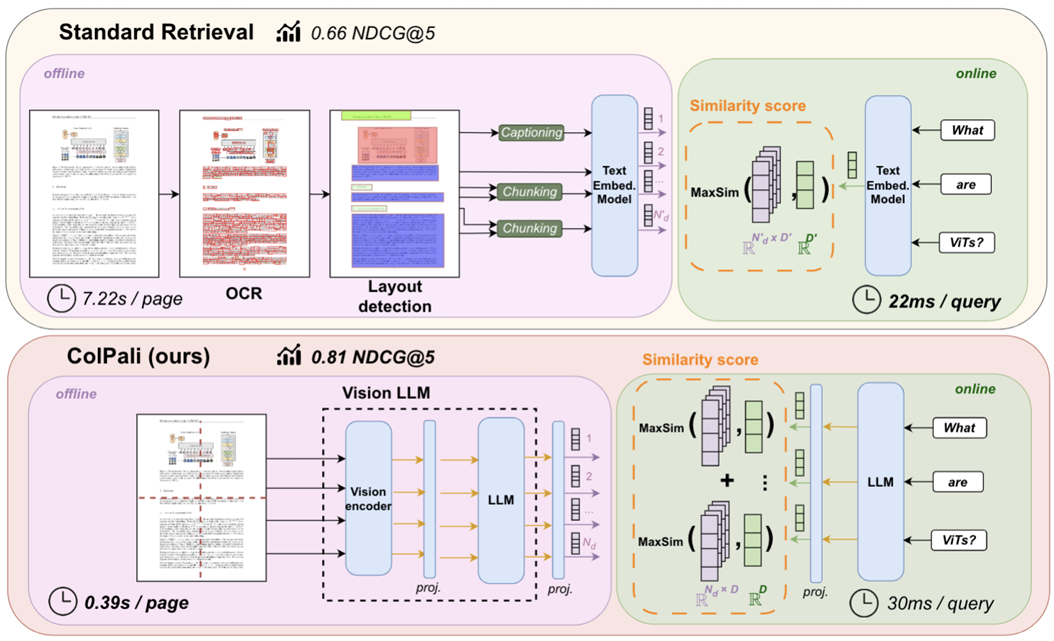
\includegraphics[width=0.9\columnwidth]{survey/figures/ColPali.png}
    \caption[ColPali late-interaction retrieval]{ColPali late-interaction retrieval for visually rich document pages. Query-token embeddings are matched against patch-level page embeddings using \emph{MaxSim}, producing a relevance score that preserves fine-grained alignment between query terms and local page regions.}
    \label{fig:colpali}
\end{figure}

\paragraph{Relation-aware retrieval.} Relation-aware methods retrieve along explicit document structure rather than scoring passages independently. Tree-based variants extract section hierarchies and outlines and group passages along semantic boundaries so retrieved chunks preserve parent context, with some routing queries through dual in-page and cross-page indices to recover both local and global evidence~\cite{shin2026multidocfusion, sun2025docagent, gong2026mhier}. Graph-based variants treat headings, entities, and cross-references as graph nodes with typed edges, so controllers or retrievers can traverse from one passage to related ones rather than relying on similarity alone; extensions add logical relevance scoring or query-conditioned graph construction to bias traversal toward inferentially connected nodes~\cite{wang2024knowledge, wu2025molorag, zhang2026mldocrag}. Relation-aware methods recover references that similarity scoring misses, at the cost of construction overhead, dependence on parser quality, and traversal cost that grows with the multi-hop count required to answer the question.

\subsection{Reasoning Strategies}
\label{sec:tf-reasoning}
Reasoning strategies act over a single fixed evidence buffer assembled prior to the reasoning call. The buffer may be the full document representation, a retrieved subset, or the output observed at one step of an agentic loop; the unifying property is that the reasoning step itself does not acquire new evidence, which makes these strategies independent of architectural family. They range from purely prompted interventions to strategies requiring changes to decoding, sampling, or control flow, but none updates model parameters. We cover the mainstream reasoning paradigms below.

\paragraph{Sequential Reasoning.} A single reasoning thread proceeds linearly, optionally revising itself as it goes. \textit{Chain-of-Thought} (CoT) prompting~\cite{wei2022chain} elicits intermediate reasoning before the final answer, which in MP-VRDU binds evidence from different pages step by step, mitigates attention dilution over long inputs, externalises the reasoning trace for verification, and decomposes multi-hop questions into single-hop steps~\cite{jia2025leopard, xiong2026docr1}. Because it operates only over the assembled buffer, its contribution lies in how faithfully that evidence is used rather than in recovering evidence the buffer omits: missing evidence cannot be reasoned back into existence. \textit{Self-Reflection} extends the single thread with iterative revision, having the model audit or refine its own answer against the buffer, optionally conditioned on feedback from a verifier or critic step~\cite{shinn2023reflexion, jain2025simpledoc, wang2025vidorag}. This reduces single-pass error at the cost of additional rounds and a self-evaluation signal whose reliability bounds the gains.

\begin{figure}[h]
    \centering
    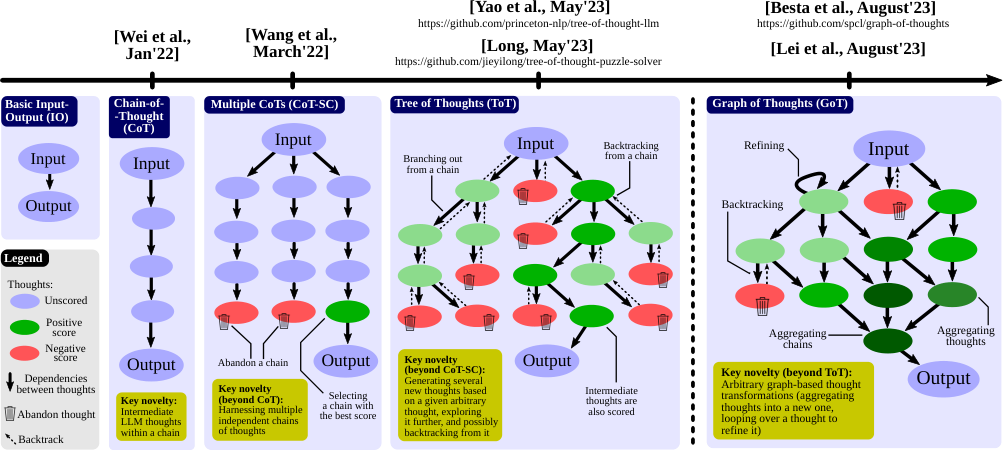
\includegraphics[width=\columnwidth]{survey/figures/prompting.png}
    \caption{Evolution of reasoning topologies used in prompting schemes. Extracted from Besta et al.~\cite{besta2025demystifying}. Only CoT is used pervasively in MP-VRDU; this diagram is for illustration purposes only.}
    \label{fig:reasoning_topologies}
\end{figure}

\paragraph{Parallel Exploration.} Several reasoning paths are produced independently and combined into one answer. \textit{Self-Consistency}~\cite{wang2023self} samples multiple chains and selects the majority answer, trading inference cost for robustness against single-chain failures, with sampling-adjudication variants replacing the majority vote with an LLM judge that compares reasoning paths and selects the most consistent conclusion~\cite{zhu2026doclens}, and parallel-pipeline variants enforcing consistency across modality-specific chains rather than across samples of one chain~\cite{suri2025visdom}. \textit{Tree-of-Thoughts} (ToT)~\cite{yao2023tree} instead explores reasoning branches with backtracking, but has seen limited uptake in MP-VRDU, where evidence sparsity rather than search-space branching is the dominant difficulty. These patterns are independent of architectural family: they can wrap a single retrieval-augmented forward pass or operate inside one step of an adaptive-trajectory loop, in which case the loop and the within-step pattern compound their effects on robustness and cost.

\subsection{Agentic Methods}
\label{sec:tf-agentic}
Agentic methods distribute the MP-VRDU workflow across one or more LLM-instantiated controllers, either iterating evidence acquisition under inference-time control or coordinating across specialised roles. We note that \textit{agentic} is used ambiguously in the MP-VRDU literature, covering both systems whose controller selects actions at inference time, following the framing by \citeauthor{plaat2025agentic} and \citeauthor{wang2024survey}, and systems composed of multiple LLM-instantiated agents in fixed roles; we treat both senses here, following the architectural distinction in \S\ref{sec:arch-ra}--\S\ref{sec:arch-agent}.

\paragraph{ReAct and Tool-Augmented Reasoning.} ReAct prompting~\cite{yao2023react} augments the action space with language thoughts, interleaving thought-action emissions in a single stream whose observations feed the next step, letting a single controller acquire evidence during inference rather than reason over a fixed buffer. The action space takes two forms in MP-VRDU. Document-side tool calls invoke external retrievers, parsers, or OCR engines, with each round concentrating on a chosen page or region~\cite{sun2025docagent, wu2025doc}, lifting the single-step recall ceiling of retrieval-augmented pipelines at the cost of tool latency and compounding error from early wrong actions. Structured navigation instead operates over a pre-built document representation, with the controller selecting which node, section, or page to inspect next~\cite{zheng2026doc}, which trades dependence on external tool fidelity for dependence on the quality of the representation built at index time. Adaptive-trajectory systems that lack the thought-action schema, such as those built on reflection-style iterative refinement~\cite{jain2025simpledoc}, share the iterative control regime without being ReAct in the strict sense.

\begin{figure}[h]
    \centering
    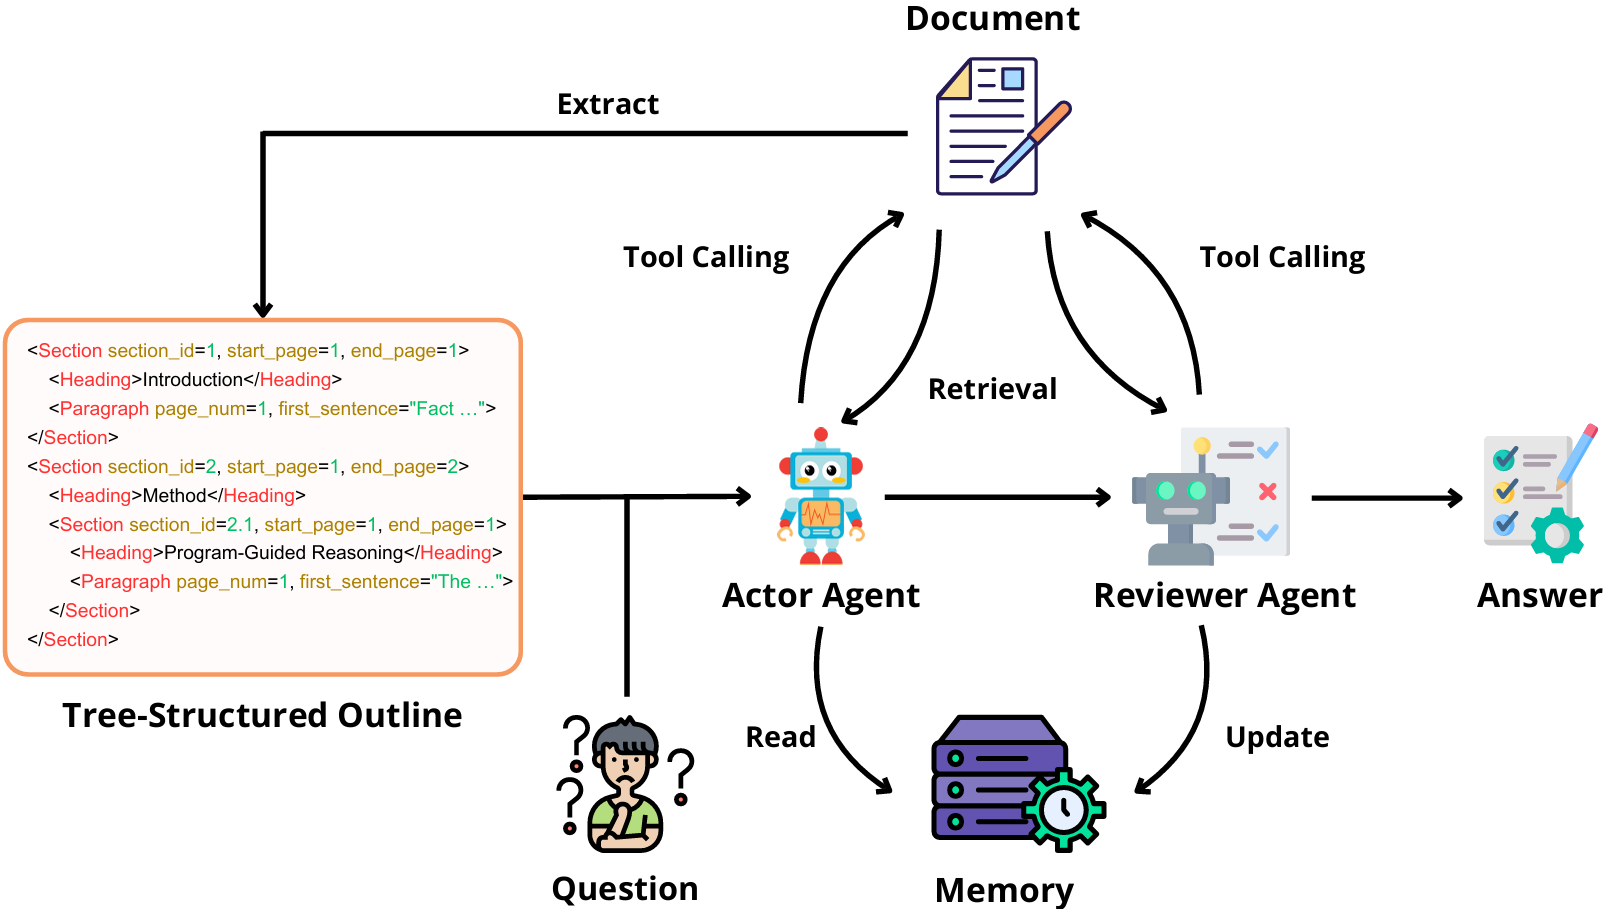
\includegraphics[width=0.75\columnwidth]{survey/figures/docagent_structure.png}
    \caption{Architecture of DocAgent. Included for illustrative purposes. Extracted from Yang et al.~\cite{sun2025docagent}.
    ``We first construct the document outline as a compact XML tree structure. An actor agent processes the outline and question as input, leveraging retrieval tools to extract relevant content for answering the question. Next, an evaluator agent reviews the initial response. If a correction is necessary, the actor agent's memory is updated through reflection, facilitating knowledge transfer across tasks.''}
    \label{fig:docagent_decomposition}
\end{figure}

\paragraph{Agentic Decomposition.} Agentic decomposition distributes the workflow across multiple controllers whose interaction pattern, rather than a single monolithic controller, drives evidence gathering and answer synthesis. Each controller operates on a narrower input and clearer objective than a single backbone tasked with the entire workflow, mitigating the cognitive overload that arises when one model must locate, read, verify, and answer over a long multimodal document~\cite{yu2025visual}. Two patterns recur. \textit{Modality-specialised} decomposition assigns separate controllers to text and visual evidence and adds a synthesis controller that reconciles their outputs, preserving single-modality reading fidelity at the cost of a reconciliation step that lacks access to the original document~\cite{han2025mdocagent, duan2025m2rag}. \textit{Role-specialised} decomposition assigns controllers to procedural stages such as planning, execution, verification, and synthesis, with explicit routing between stages when a downstream controller detects an error~\cite{yu2025visual, sun2025docagent}. Separating judgement from generation reduces the cognitive blind spots of self-correction, but introduces inter-controller compatibility costs and a recall ceiling bounded by upstream stages.

% \subsection{Coarse-to-Fine Reasoning}
% \label{sec:tf-coarse}
% Coarse-to-fine reasoning is the most widely adopted structured-reasoning pattern in the surveyed corpus, appearing across MLLM-centric, retrieval-augmented, and adaptive-trajectory systems (Table~\ref{tab:model_survey_arch}). The pattern decomposes document-scale reasoning into successive stages of decreasing scope: an initial pass over the whole document or a broad candidate set identifies regions likely to contain answer-relevant evidence, and subsequent passes restrict attention to those regions at higher fidelity. Three implementations recur. \textbf{Page to region} variants first select candidate pages from the document, then reason over each candidate at higher fidelity or with more detailed analysis before answering~\cite{shi2026urag, xiong2026docr1, yan2026docseeker, gong2026mhier}, with some realisations operating across discrete passes and others embedding the pattern within the layers of a single MLLM. \textbf{Retrieve, rerank, then read} variants extend the pattern across the retrieval stack, with an initial dense or sparse retrieval returning a broad candidate set, a reranker narrowing it through LLM-based scoring, and the generator reading only the final subset~\cite{zhang2024cream, xu2025mm, shin2026multidocfusion, zhang2026mldocrag}. \textbf{Plan then execute} variants instantiate the pattern at the controller level, first producing an evidence-acquisition plan that identifies which pages or regions to inspect, then executing the plan in sequence with iterative refinement~\cite{zheng2026doc, sun2025docagent, fu2026dmap}. Across all three, early stages operate over compact representations and late stages at full fidelity over a narrowed scope, making coarse-to-fine a natural fit for the cost structure of MP-VRDU, though errors at an early stage are unrecoverable at later stages since later stages see only what was admitted upstream.

\section{Training Strategies}
\label{sec:training}

VRDU training follows a stepwise pipeline established in the single-page setting~\cite{ding2026survey}: self-supervised pretraining instils document reading through objectives such as masked information modelling and cross-modality alignment, instruction tuning aligns outputs with user queries, and supervised fine-tuning adapts the model to target tasks. MP-VRDU inherits this pipeline but concentrates its effort at the later stages, since document-scale pretraining corpora remain scarce and most systems adopt backbones already pretrained on single-page data, with few exceptions targeting cross-page objectives directly~\cite{hu2025mplug, duan2025docopilot}. Fine-tuning instead carries the weight, scaled by LVLM-synthesised supervision (\S\ref{sec:datasets}), with reinforcement learning increasingly layered above it. Training therefore internalises the evidence-management decisions of \S\ref{sec:inference-time} into model parameters, supplying capabilities that prompting cannot: cross-page evidence selection (\S\ref{sec:train-retrieval}), document-scale reasoning over assembled evidence (\S\ref{sec:train-reasoning}), and reliable agentic acquisition (\S\ref{sec:train-agentic}). Two cross-cutting techniques recur across all three (\S\ref{sec:train-crosscutting}).

\subsection{Trained Retrieval Components}
\label{sec:train-retrieval}

Off-the-shelf encoders such as ColPali and ColQwen~\cite{faysse2025colpali} score each page independently against the query, so retrieved results are dominated by local query-page similarity rather than by document-level context. Retriever training has therefore explored three complementary directions. \textit{Modality-alignment} methods learn visual document embeddings that remain aligned with OCR-derived text, enabling page images to be retrieved without the storage and latency cost of the late-interaction patch-level scoring discussed in \S\ref{sec:tf-retrieval}~\cite{tanaka2025vdocrag}. \textit{Cross-page-fusion} methods enrich each page representation with neighbouring-page context, typically through a lightweight head trained with parameter-efficient methods such as LoRA~\cite{hu2022lora}, a tuning approach that adds small trainable matrices to frozen weights; the result makes evidence distributed across adjacent or related pages retrievable as a unit rather than as a set of independently-ranked passages~\cite{qian2026accurate}. \textit{Logical-relevance} methods train graph-based scorers to rank pages not only by embedding similarity but also by their role in cross-page reasoning paths, turning retrieval into a learned multi-hop walk rather than a single-step similarity match~\cite{wu2025molorag}. The three directions are not interchangeable: modality-alignment improves retrieval throughput, cross-page-fusion improves recall on adjacent evidence, and logical-relevance improves recall on inferentially-connected evidence.

\subsection{Trained Reasoning over Assembled Evidence}
\label{sec:train-reasoning}

Prompted reasoning leaves quality sensitive to prompt design and base-model behaviour, motivating approaches that train the reasoning component directly so the model produces structured reasoning trajectories on its own rather than relying on a prompt schema imposed at inference time. Three patterns recur. \textit{Trace-imitation} variants supervise the backbone on demonstration chains wrapped in fixed schema tags such as \texttt{<think>}, \texttt{<evidence>}, and \texttt{<answer>}, optionally extended across procedural stages such as plan, execute, integrate, and verify; staged training pipelines further refine through Direct Preference Optimisation (DPO), a method that trains on pairs ranked by preference rather than scalar rewards to prefer faithful chains over hallucinated shortcuts~\cite{guo2026end}. \textit{Reward-driven} variants optimise the reasoning policy directly with Group Relative Policy Optimisation (GRPO), a reinforcement-learning method that compares grouped rollouts to compute relative rewards; the composite reward typically combines answer accuracy, evidence-page recall, and format compliance, and the policy is often warm-started from a trace-imitation stage rather than learned from scratch~\cite{xiong2026docr1}. The two are therefore sequential rather than alternative, with reward-driven training refining what imitation alone cannot supply. \textit{Uncertainty-calibration} variants take a different route, training an aggregation head that selects across candidate outputs by calibrated uncertainty rather than internalising the reasoning chain itself, which yields a learned self-consistency signal that scales to long documents under tight parameter budgets and avoids the cost of sampling multiple chains at test time~\cite{hannan2026docslm}.

\subsection{Trained Agentic Methods}
\label{sec:train-agentic}
Prompt-only agentic control is unreliable on smaller open-weight backbones, which cannot consistently follow ReAct schemas, select among tool calls, or terminate trajectories reliably. Two patterns recur. \textit{Trajectory-distillation} variants clone agentic trajectories from a stronger teacher model through supervised fine-tuning on think-action-observation turns, with teacher rollouts collected in closed-loop interaction and filtered for format validity, answer correctness, and evidence coverage; this trains the smaller model to match the trajectory shape of the larger teacher rather than learning the underlying policy from scratch, with some variants additionally conditioning tool selection on a learned representation of the agent's current goal so that action choices reflect the trajectory's evolving intent rather than only its most recent observation~\cite{zhang2026docdancer}. \textit{Reinforcement-learned} variants optimise the agentic policy directly against trajectory-level rewards that combine answer correctness, evidence recall, and tool-use shape, often pairing a supervised warm-start with GRPO over a constrained action space such as retrieval and page-fetch calls; learned termination is a recurring concern, with entropy-based stopping letting the trained model commit to an answer once its prediction confidence stabilises rather than running for a fixed number of rounds~\cite{zheng2026doc}. Multi-agent variants extend this further by allocating sample budgets per controller across procedural roles such as planner, executor, judge, and answerer rather than running every controller at a fixed budget, spending more compute on the role that the question's difficulty most stresses~\cite{yu2025visual}. The surveyed evidence does not cleanly separate distillation from reinforcement learning, since reported comparisons confound the training objective with backbone, reward design, and trajectory budget.

\subsection{Cross-Cutting Training Techniques}
\label{sec:train-crosscutting}

\begin{figure}[h]
    \centering
    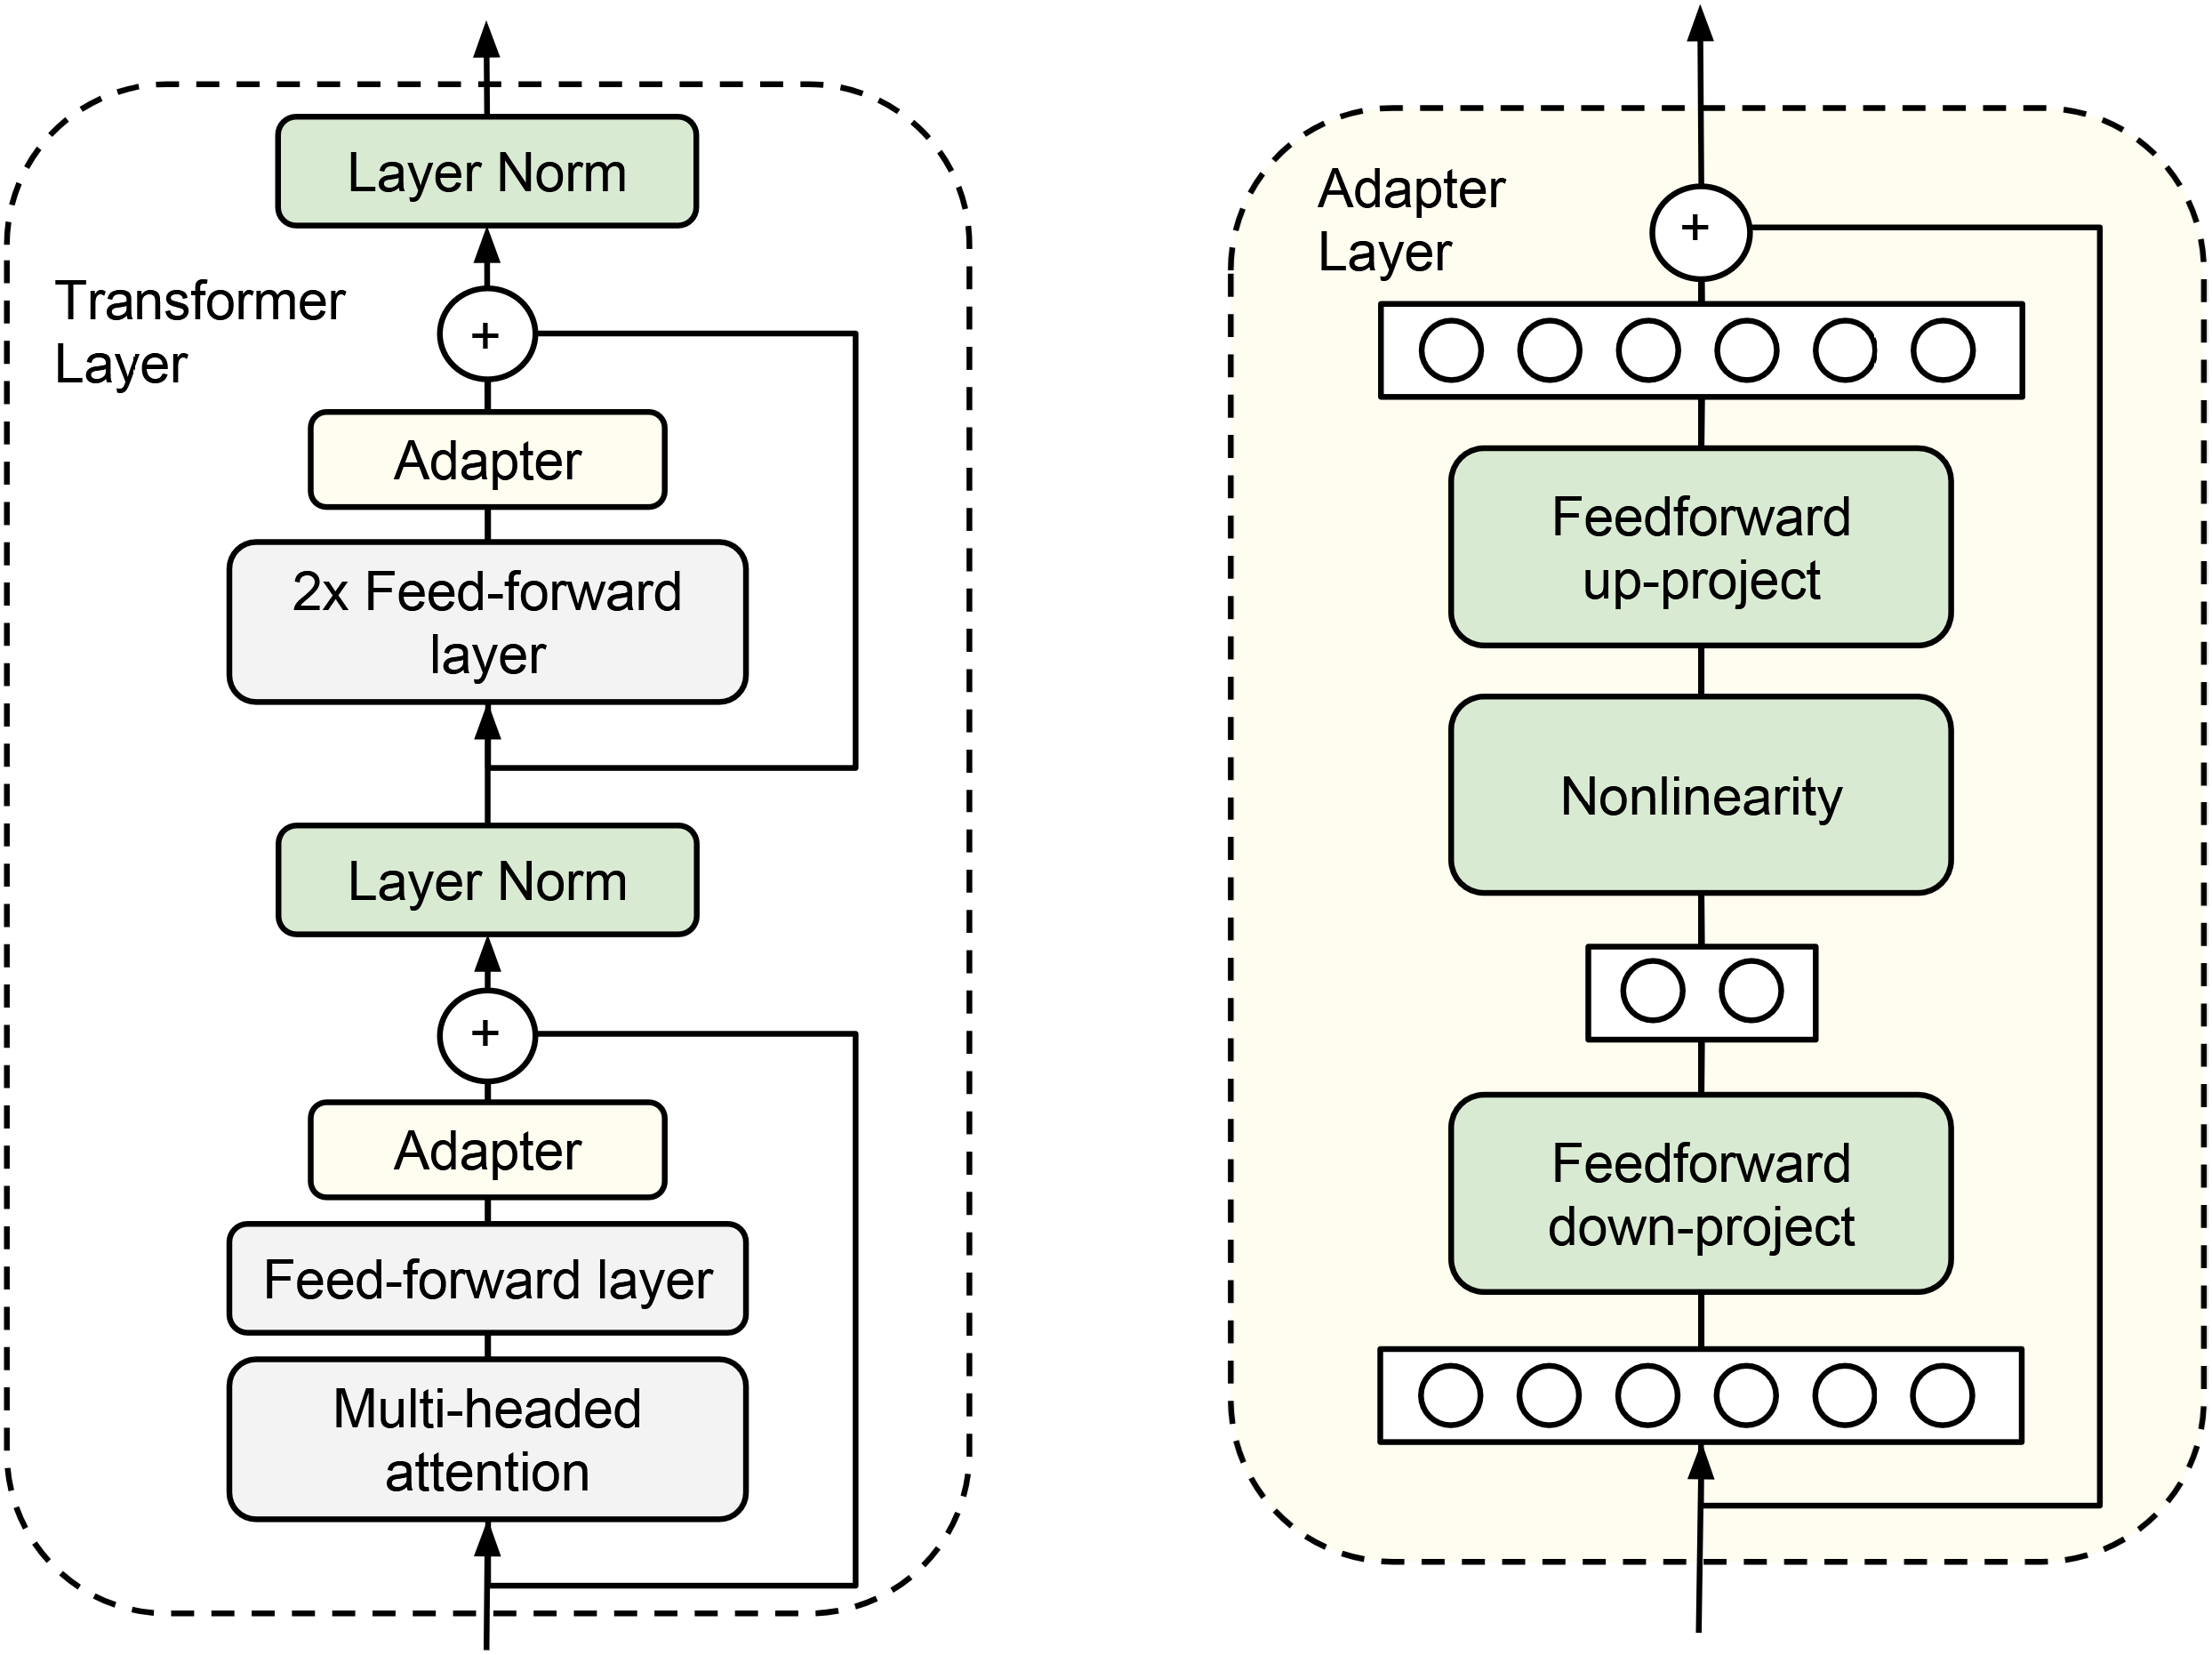
\includegraphics[width=0.6\columnwidth]{survey/figures/houlsby_adapter.png}
    \caption{Adapter-based parameter-efficient tuning. Included for illustrative purposes. Two adapter modules are inserted into each transformer layer (left); each is a small bottleneck that down-projects to a low dimension, applies a nonlinearity, up-projects back, and adds the result to its input through a residual connection (right). During training the backbone weights are frozen and only the adapter modules and layer norms are updated. Adapted from Houlsby et al.~\cite{houlsby2019peft}.}
    \label{fig:houlsby_adapter}
\end{figure}

Two techniques recur across retriever, reasoner, and orchestration policy training, independent of which component is being optimised. \textbf{Parameter-efficient tuning} is the dominant adaptation strategy: full backbone fine-tuning is prohibitive at long-document context lengths and risks erasing pretrained capabilities, so most systems freeze the backbone and train lightweight modules through LoRA matrices, projection heads, or task-specific adapters~\cite{zhu2025simple, zhang2024cream, qian2026accurate, zhang2026docdancer}. The adapted module varies by target: layout-token modules inject structural information~\cite{zhu2025simple}, projection heads align frozen retrievers with downstream readers~\cite{qian2026accurate}, and LoRA matrices adapt reasoning or trajectory behaviour without touching backbone weights~\cite{zhang2024cream, zhang2026docdancer}; the choice between parameter-efficient and full fine-tuning is more often a compute-budget decision than a target-component one. \textbf{Multi-stage curriculum training} addresses a different concern: several systems converge on curricula that start on single-page or local objectives before introducing document-scale supervision, exploiting the fact that text reading and layout understanding transfer from single-page data while cross-page integration must be learned separately~\cite{hu2025mplug, hannan2026docslm}. Later stages typically add streaming, abstention, or evidence-grounding objectives once foundational reading capabilities are established, with the longest schedules layering five or more stages from image-OCR alignment through to streaming-abstention calibration. Their recurrence across otherwise dissimilar systems indicates that cross-page integration does not emerge from single-page supervision alone.

\section{Datasets}
\label{sec:datasets}
Multi-page documents impose a structural constraint absent from the single-page setting: per-page annotation does not scale to the page counts typical of MP-VRDU, and multi-page corpora are scarce because long PDFs are harder to source, license, and parse than single pages. This constraint shapes the three roles a dataset can play, pretraining (PT), supervised fine-tuning (SFT), and benchmarking (BM), differently from SP-VRDU, and several datasets occupy more than one role across different systems.

% -----------------------------------------------------------------------------
% Auto-generated by summary_datasets_convert.py -- do NOT edit manually.
% Re-generate:  python3 summary_datasets_convert.py datasets_summary.csv datasets_summary.tex
%
% Required packages (add to your preamble):
%   \usepackage{booktabs}
%   \usepackage{array}
%   \usepackage{xcolor}
%   \usepackage{colortbl}
%   \usepackage{caption}
%   \usepackage{adjustbox}
%   \usepackage{natbib}      % for \citeyear  (or use biblatex)
% -----------------------------------------------------------------------------

\definecolor{sectionbg}{gray}{0.88}

% -- tab:dataset_survey -----------------------------------------------
\begin{table*}[h]
\centering
\scriptsize
\captionsetup{font=small}
\setlength{\tabcolsep}{3pt}
\renewcommand{\arraystretch}{0.86}
\begin{adjustbox}{width=\textwidth}
\begin{tabular}{l c c l l r r r l}
\toprule
\textbf{Dataset} & \textbf{Pages} & \textbf{Type} & \textbf{Venue} & \textbf{Domain} & \textbf{\#\,Docs} & \textbf{Avg\,Pages} & \textbf{\#\,Q/A} & \textbf{Multi/S Hop} \\
\midrule

  DocVQA~(\citeyear{mathew2021docvqa}) & SP & PT+BM & WACV & Industry & 12767 & -- & 50,000 & S \\
  FeTaQA~(\citeyear{nan2022fetaqa}) & SP & PT+BM & TACL & Wikipedia tables & 10330 & -- & 10,330 & M \\
  InfographicVQA~(\citeyear{mathew2022infographicvqa}) & SP & PT+BM & WACV & Infographics & 5,485 & -- & 30,035 & M+S \\
  PDF-VQA Task A~(\citeyear{ding2023pdf}) & SP & PT+BM & ECML-PKDD & Biomedical & -- & -- & 81,085 & S \\
  PDF-VQA Task B~(\citeyear{ding2023pdf}) & SP & PT+BM & ECML-PKDD & Biomedical & -- & -- & 53,872 & S \\
  TabFact~(\citeyear{chen2020tabfact}) & SP & PT+BM & ICLR & Wikipedia tables & 16573 & -- & 118,275 & M+S \\
  TextVQA~(\citeyear{singh2019towards}) & SP & PT+BM & CVPR & Scene-text images & 28408 & -- & 45,336 & S \\
  VisualMRC~(\citeyear{tanaka2021visualmrc}) & SP & PT+BM & AAAI & Webpages & 10197 & -- & 30,562 & M+S \\
  WikiTableQuestions~(\citeyear{pasupat2015compositional}) & SP & PT+BM & ACL & Wikipedia tables & 2108 & -- & 22,033 & M \\
  ChartQA~(\citeyear{masry2022chartqa}) & SP & BM & ACL & Charts & 20882 & -- & 32,719 & M+S \\
  DocGenome~(\citeyear{xia2024docgenome}) & MP & PT+BM & NeurIPS & Academic Paper & 500000 & 13 & 3000 & M+S \\
  DuReaderVis~(\citeyear{qi2022dureader}) & MP & PT+BM & ACL & Cross-domain & 158000 & -- & 15,000 & S \\
  Kleister-Charity~(\citeyear{stanislawek2021kleister}) & MP & PT+BM & ICDAR & Financial & 2778 & 22.19 & 21,612 & S \\
  Kleister-NDA~(\citeyear{stanislawek2021kleister}) & MP & PT+BM & ICDAR & Legal & 540 & 5.98 & 2,160 & S \\
  M-LongDoc~(\citeyear{chia2025m}) & MP & PT+BM & EMNLP & Cross-domain & 180 & 210.8 & 851 & S \\
  MMVQA~(\citeyear{ding2024mmvqa}) & MP & PT+BM & IJCAI & Biomedical & 3146 & 9.6 & 262,928 & M+S \\
  MP-DocVQA~(\citeyear{tito2023hierarchical}) & MP & PT+BM & PR & Industry & 5928 & 8.27 & 46,176 & S \\
  MultiHiertt~(\citeyear{zhao2022multihiertt}) & MP & PT+BM & ACL & Financial reports & 2513 & \textasciitilde{}2.5 & 10,440 & M \\
  PaperPDF~(\citeyear{xie2026pdf}) & MP & PT+BM & preprint & Academic Paper & -- & -- & 1,110,000 & M+S \\
  PDF-VQA Task C~(\citeyear{ding2023pdf}) & MP & PT+BM & ECML-PKDD & Biomedical & 1147 & \textasciitilde{}10 & 5,653 & M \\
  QASPER~(\citeyear{dasigi2021dataset}) & MP & PT+BM & NAACL & Academic Paper & 1585 & \textasciitilde{}8 & 5,049 & M \\
  SlideVQA~(\citeyear{tanaka2023slidevqa}) & MP & PT+BM & AAAI & Presentations & 2619 & 20 & 14,484 & M+S \\
  MP-DocStruct1M~(\citeyear{hu2025mplug}) & MP & PT & ACL & Cross-domain & -- & -- & 1,113,259 & S \\
  OpenDocVQA~(\citeyear{tanaka2025vdocrag}) & MP & SFT+BM & CVPR & Cross-domain & -- & -- & -- & M+S \\
  CoR-Dataset~(\citeyear{guo2026end}) & MP & SFT & preprint & Cross-domain & -- & -- & 26,088 & M+S \\
  Doc-750K~(\citeyear{duan2025docopilot}) & MP & SFT & CVPR & Academic Paper & -- & -- & 758,000 & M+S \\
  MHDocVQA~(\citeyear{tanaka2025vdocrag}) & MP & SFT & CVPR & Cross-domain & -- & 9.5 & 38,020 & M \\
  MP-DocReason51K~(\citeyear{hu2025mplug}) & MP & SFT & ACL & Cross-domain & -- & -- & 51,754 & M+S \\
  BRIDGE~(\citeyear{xiang2026bridge}) & MP & BM & preprint & Academic Paper & 262 & -- & 11,857 & M \\
  DocBench~(\citeyear{zou2024docbench}) & MP & BM & preprint & Cross-domain & 229 & -- & 1,102 & S \\
  DUDE~(\citeyear{landeghem2023document}) & MP & BM & ICCV & Cross-domain & 5019 & 5.72 & 41,541 & M+S \\
  FetaTab~(\citeyear{hui2024uda}) & MP & BM & NeurIPS & Wikipedia Articles & 871 & \textasciitilde{}11 & 1,016 & S \\
  LongDocURL~(\citeyear{deng2025longdocurl}) & MP & BM & ACL & Cross-domain & 396 & 85.6 & 2,325 & M+S \\
  M3DocVQA~(\citeyear{cho2025m3docvqa}) & MP & BM & CVPR & Wikipedia Articles & 3368 & 12.2 & 2,441 & M+S \\
  MM-NIAH~(\citeyear{wang2024mmniah}) & MP & BM & NeurIPS & Synthetic & -- & -- & 16,486 & M+S \\
  MMDocIR~(\citeyear{dong2025mmdocir}) & MP & BM & ACL & Cross-domain & 313 & 65.1 & 1,658 & M+S \\
  MMLongBench~(\citeyear{wang2025mmlongbench}) & MP & BM & NeurIPS & Cross-domain & -- & -- & 13,331 & M+S \\
  MMLongBench-Doc~(\citeyear{ma2024mmlongbench}) & MP & BM & NeurIPS & Cross-domain & 135 & 47.5 & 1,082 & M+S \\
  PaperTab~(\citeyear{hui2024uda}) & MP & BM & NeurIPS & Academic Paper & 307 & \textasciitilde{}11 & 393 & M+S \\
  PaperText~(\citeyear{hui2024uda}) & MP & BM & NeurIPS & Academic Paper & 1087 & \textasciitilde{}11 & 2,804 & M+S \\
  ViDoSeek~(\citeyear{wang2025vidorag}) & MP & BM & EMNLP & Cross-domain & -- & -- & 1,200 & M+S \\
  VisDoMBench~(\citeyear{suri2025visdom}) & MP & BM & NAACL & Cross-domain & 1277 & 19.11 & 2,271 & M+S \\
  VisR-Bench~(\citeyear{chen2025sv}) & MP & BM & ICLR & Cross-domain & 226 & -- & 471 & M+S \\
  DocStruct4M~(\citeyear{hu2024mplug}) & MP+SP & PT+SFT & EMNLP & Cross-domain & -- & -- & 4,000,000 & M+S \\
  TAT-DQA~(\citeyear{zhu2022towards}) & MP+SP & PT+BM & ACM & Financial reports & 2758 & 1.33 & 16,558 & M \\
  InstructDoc~(\citeyear{tanaka2024instructdoc}) & MP+SP & SFT & AAAI & Cross-domain & -- & -- & -- & M+S \\
  Leopard-Instruct~(\citeyear{jia2025leopard}) & MP+SP & SFT & TMLR & Cross-domain & -- & -- & 925,000 & M+S \\

\bottomrule
\end{tabular}
\end{adjustbox}
\caption{Datasets referenced in the MP-VRDU survey. \textbf{Pages}: document scope (MP\,=\,Multi-Page, SP\,=\,Single-Page, MP+SP\,=\,Mixed). \textbf{Type}: dataset role -- PT (Pretraining), SFT (Supervised Fine-Tuning), BM (Benchmark), and combinations. \textbf{Hop}: question-hop type (Single, Multi, or both). `--' indicates not reported.}
\label{tab:dataset_survey}
\end{table*}


\subsection{Pretraining}
\label{sec:dataset-pt}
Pretraining is the exception rather than the norm in MP-VRDU. Only a handful of page-to-document and MLLM-centric systems pretrain or continue-train a backbone at all; retrieval-augmented and agentic pipelines inherit pretrained vision-language backbones and skip the stage entirely. Two factors explain its scarcity. Document-scale pretraining is computationally expensive, and genuinely multi-page corpora are few, so most systems that pretrain fall back on single-page archives or repurpose single-page data. Early work drew on single-page OCR archives such as IIT-CDIP~\citep{lewis2006building} and OCR-IDL~\citep{biten2022ocr}, which supply text-recognition supervision but no cross-page structure. Genuinely multi-page corpora have appeared only recently: DocStruct4M~\citep{hu2024mplug} mixes single- and multi-page samples with structure-aware parsing supervision, while the purely multi-page MP-DocStruct1M~\citep{hu2025mplug}, Doc-750K~\citep{duan2025docopilot}, and PaperPDF~\citep{xie2026pdf} support continued pretraining over genuine multi-page inputs. Where multi-page pretraining does occur, its objective has shifted from text recognition toward structure-aware supervision, but the corpus as a whole shows that most cross-page capability is instilled at fine-tuning rather than pretraining.

\subsection{Supervised Fine-Tuning}
\label{sec:dataset-sft}
Because per-page human annotation does not scale, supervised fine-tuning has converged on two strategies, often combined within one system. The first aggregates publicly released question-answer collections into broad instruction mixes spanning heterogeneous question and answer types~\citep{tanaka2024instructdoc, jia2025leopard, hu2025mplug, duan2025docopilot}. The second curates a bespoke corpus for the system under study, typically synthesised by a strong vision-language model that writes question-answer pairs, reasoning traces, or agent trajectories over scraped PDFs~\citep{xie2026pdf, tanaka2025vdocrag, wu2025molorag, zhang2026docdancer, guo2026end}. Synthetic generation has become the dominant scaling path for fine-tuning data, and its underlying PDF pools are typically drawn from the same scientific archives, slide repositories, and benchmark sources that also supply evaluation. Layered above this, a growing body of work applies reinforcement or preference learning with rewards that credit correct evidence-page citation, faithful chain-of-thought structure, or appropriate tool use rather than final-answer accuracy alone~\citep{xiong2026docr1, guo2026end, yan2026docseeker}. These reinforcement pools remain small relative to the supervised mixes that precede them, indicating that reinforcement signals shape behaviour, instilling evidence grounding, output formatting, and multi-step reasoning, rather than scaling the data itself.

\subsection{Benchmarking}
\label{sec:dataset-bm}
Benchmarks have evolved through several tiers that accumulated rather than replaced one another. Single-page extractive evaluation on DocVQA~\citep{mathew2021docvqa}, InfographicVQA~\citep{mathew2022infographicvqa}, and ChartQA~\citep{masry2022chartqa} persists as a per-page baseline, and mid-length corpora such as MP-DocVQA~\citep{tito2023hierarchical}, DUDE~\citep{landeghem2023document}, and SlideVQA~\citep{tanaka2023slidevqa} extend the same extractive formats into a few-page setting. Long-document multimodal benchmarks then introduced documents whose total length routinely exceeds backbone context windows and whose evidence requires cross-page integration over mixed text, tables, charts, and figures, including MMLongBench-Doc~\citep{ma2024mmlongbench}, LongDocURL~\citep{deng2025longdocurl}, DocBench~\citep{zou2024docbench}, and M-LongDoc~\citep{chia2025m}. Retrieval-oriented benchmarks such as UDA-Benchmark~\citep{hui2024uda} and DocLens~\citep{zhu2026doclens} additionally score evidence-page selection and layout-level localisation alongside answer accuracy, and the most recent additions push into cross-document settings, including M3DocRAG~\citep{cho2024m3docrag}, ViDoRAG~\citep{wang2025vidorag}, and VDocRAG~\citep{tanaka2025vdocrag}. Despite this proliferation, evaluation in practice has consolidated around a small set of long-document and mid-length benchmarks that recur in most reported comparisons. That the same scarce pool of source PDFs supplies both synthetic fine-tuning data and evaluation is a contamination risk we return to in \S\ref{sec:conc_supervision}.

\section{Conclusion}
\label{sec:survey-conc}

This chapter established MP-VRDU as a distinct document-understanding problem organised around evidence management. It introduced a taxonomy of four architectural families and surveyed the multimodal representations, inference-time strategies, training approaches, datasets, and evaluation practices used across the field. Across these dimensions, the literature consistently shows that long-document performance depends not only on backbone capability, but on how evidence is preserved, selected, compressed, and integrated across pages. The broader challenges and future research directions that emerge from this survey are discussed in Chapter~\ref{ch:conclusion}.

% ─────────────────────────────────────────────────────────────────────────────
% MP-VRDU Survey Taxonomy Figure
%
% Required packages (add to your preamble if not already present):
%   \usepackage{tikz}
%   \usepackage{forest}
%   \usepackage{xcolor}
%   \usepackage{adjustbox}
%   \usetikzlibrary{arrows.meta}
% ─────────────────────────────────────────────────────────────────────────────

% ── Column widths — edit these to resize boxes per column. ───────────────────
% If the text exceeds the width, it will wrap onto a second (or third) line.
\newcommand{\TaxRootWidth}{34mm}
\newcommand{\TaxSectionWidth}{22mm}
\newcommand{\TaxSubsectionWidth}{42mm}
\newcommand{\TaxIdeaWidth}{32mm}
\newcommand{\TaxLeafWidth}{42mm}


% ── Spacing parameters. ──────────────────────────────────────────────────────
% \TaxEdgeStub: length of the horizontal stub leaving each parent box before
% the edge turns vertical. Increase if the perpendicular gap looks too small.
\newcommand{\TaxLevelSep}{14pt}
\newcommand{\TaxSiblingSep}{1.2pt}
\newcommand{\TaxEdgeStub}{6pt}

% ── Colours — edit to recolour the figure. ───────────────────────────────────
\definecolor{nodebg}{HTML}{E8E8E8}
\definecolor{leafbg}{HTML}{D6E6F4}

\begin{figure*}[p]
\centering
\begin{adjustbox}{max totalsize={\textwidth}{0.92\textheight},center}
\begin{forest}
  for tree={
    grow'=east,
    parent anchor=east,
    child anchor=west,
    anchor=west,
    align=left,
    edge={-{Stealth[length=3pt]}, thin, gray!55},
    edge path={
      \noexpand\path[\forestoption{edge}]
        (!u.parent anchor) -- +(\TaxEdgeStub,0) |- (.child anchor)\forestoption{edge label};
    },
    l sep=\TaxLevelSep,
    s sep=\TaxSiblingSep,
    font=\scriptsize,
    rounded corners=2pt,
    draw=gray!50,
    inner sep=2.5pt,
    inner xsep=4pt,
    fill=nodebg,
  },
  % Root: rotated 90° banner. parent anchor=south puts the outgoing edge on
  % the visible east of the rotated box, so the line does not overlap the box.
  where level=0{
    font=\small\bfseries,
    align=center,
    rotate=90,
    anchor=center,
    parent anchor=south,
    text width=\TaxRootWidth,
  }{},
  % Section column.
  where level=1{font=\scriptsize\bfseries, text width=\TaxSectionWidth, align=left}{},
  % Subsection column.
  where level=2{text width=\TaxSubsectionWidth, align=left}{},
  % Idea column (level 3 non-leaf; level-3 leaves in §7/§8 fall through to leaf rule below).
  where level=3{text width=\TaxIdeaWidth, align=left}{},
  % Leaf rule comes LAST so it overrides any level-specific width above.
  % Applies to every node with no children (level 4 in §3–§6, level 3 in §7/§8).
  where n children=0{
    tier=leafrow,
    fill=leafbg,
    font=\tiny,
    text width=\TaxLeafWidth,
    align=left,
  }{},
  [MP-VRDU Taxonomy
    %% ── §3 Architecture ───────────────────────────────────────────────────
    [§\ref{sec:architecture}~Architecture
      [§\ref{sec:arch-p2d}~Page-to-Document
        [Summary tokens
          [{Hi-VT5~\cite{tito2023hierarchical}}]
        ]
        [Cross-page attention
          [{Arctic-TILT~\cite{borchmann2025arctic}, GRAM~\cite{blau2024gram}}]
        ]
        [Recurrent state
          [{RM-T5~\cite{dong2024multi}}]
        ]
      ]
      [§\ref{sec:arch-mllm}~MLLM-Centric
        [Lightweight projector
          [{InstructDoc~\cite{tanaka2024instructdoc}, LayTokenLLM~\cite{zhu2025simple}}]
        ]
        [Token compression
          [{mPLUG-DocOwl2~\cite{hu2025mplug}, Texthawk2~\cite{yu2024texthawk2}}]
        ]
        [Backbone fine-tuning
          [{Docopilot~\cite{duan2025docopilot}, DocR1~\cite{xiong2026docr1}}]
        ]
      ]
      [§\ref{sec:arch-ra}~Retrieval-Augmented
        [Single retriever-reader
          [{M3DocRAG~\cite{cho2024m3docrag}, VDocRAG~\cite{tanaka2025vdocrag}}]
        ]
        [Multi-component pipeline
          [{MDocAgent~\cite{han2025mdocagent}, VisDoM~\cite{suri2025visdom}}]
        ]
      ]
      [§\ref{sec:arch-agent}~Adaptive-Trajectory
        [External tool calls
          [{ViDoRAG~\cite{wang2025vidorag}, MACT~\cite{yu2025visual}}]
        ]
        [Structured navigation
          [{SimpleDoc~\cite{jain2025simpledoc}, DMap~\cite{fu2026dmap}}]
        ]
      ]
    ]
    %% ── §4 Modalities ────────────────────────────────────────────────────
    [§\ref{sec:modality}~Modalities
      [§\ref{sec:modality-text}~Text
        [Volume
          [{Arctic-TILT~\cite{borchmann2025arctic}, PDF-WuKong~\cite{xie2026pdf}}]
        ]
        [Continuity
          [{RM-T5~\cite{dong2024multi}, MultiDocFusion~\cite{shin2026multidocfusion}}]
        ]
        [Heterogeneity
          [{AVIR~\cite{li2026avir}}]
        ]
      ]
      [§\ref{sec:modality-visual}~Visual
        [Resolution (compression)
          [{Texthawk2~\cite{yu2024texthawk2}, Leopard~\cite{jia2025leopard}}]
        ]
        [Selective high-res
          [{DocSeeker~\cite{yan2026docseeker}, DocLens~\cite{zhu2026doclens}}]
        ]
        [Multi-signal competition
          [{M3DocRAG~\cite{cho2024m3docrag}, VDocRAG~\cite{tanaka2025vdocrag}}]
        ]
      ]
      [§\ref{sec:modality-structure}~Structure
        [Hierarchy \& reading order
          [{DocAgent~\cite{sun2025docagent}, DMap~\cite{fu2026dmap}}]
        ]
        [Cross-page references
          [{KGP~\cite{wang2024knowledge}, MoLoRAG~\cite{wu2025molorag}}]
        ]
        [Spanning elements
          [{MHier-RAG~\cite{gong2026mhier}, DFVC~\cite{qian2026accurate}}]
        ]
      ]
    ]
    %% ── §5 Inference-Time Adaptation ─────────────────────────────────────
    [§\ref{sec:inference-time}~Inference
      [§\ref{sec:tf-retrieval}~Retrieval \& Navigation
        [Similarity-based
          [{ColPali~\cite{faysse2025colpali}, SimpleDoc~\cite{jain2025simpledoc}}]
        ]
        [Relation-aware
          [{MultiDocFusion~\cite{shin2026multidocfusion}, MLDocRAG~\cite{zhang2026mldocrag}}]
        ]
      ]
      [§\ref{sec:tf-reasoning}~Prompted Reasoning
        [Sequential Reasoning
          [{Leopard~\cite{jia2025leopard}, MM-R5~\cite{xu2025mm}}]
        ]
        [Parallel Exploration
          [{DocLens~\cite{zhu2026doclens}, ToT~\cite{yao2023tree}}]
        ]
      ]
      [§\ref{sec:tf-agentic}~Agentic Methods
        [ReAct \& tool-augmented
          [{Doc-V*~\cite{zheng2026doc}, Doc-React~\cite{wu2025doc}}]
        ]
        [Modality-specialised
          [{MDocAgent~\cite{han2025mdocagent}, M$^2$RAG~\cite{duan2025m2rag}}]
        ]
        [Role-specialised
          [{MACT~\cite{yu2025visual}, DocAgent~\cite{sun2025docagent}}]
        ]
      ]
    ]
    %% ── §6 Training Strategies ───────────────────────────────────────────
    [§\ref{sec:training}~Training
      [§\ref{sec:train-retrieval}~Retrieval
        [Modality alignment
          [{VDocRAG~\cite{tanaka2025vdocrag}}]
        ]
        [Cross-page fusion
          [{DFVC~\cite{qian2026accurate}}]
        ]
        [Logical relevance
          [{MoLoRAG~\cite{wu2025molorag}}]
        ]
      ]
      [§\ref{sec:train-reasoning}~Reasoning
        [Trace imitation
          [{DocSeeker~\cite{yan2026docseeker}, CoR~\cite{guo2026end}}]
        ]
        [Reward-driven RL
          [{DocR1~\cite{xiong2026docr1}, MM-R5~\cite{xu2025mm}}]
        ]
        [Uncertainty calibration
          [{DocSLM~\cite{hannan2026docslm}}]
        ]
      ]
      [§\ref{sec:train-agentic}~Agentic
        [Trajectory distillation
          [{Doc-V*~\cite{zheng2026doc}, DocDancer~\cite{zhang2026docdancer}}]
        ]
        [Reinforcement-learned
          [{MM-Doc-R1~\cite{lin2026mm}, VRAG-RL~\cite{wang2025vrag}}]
        ]
      ]
      [§\ref{sec:train-crosscutting}~Cross-Cutting
        [PEFT
          [{LayTokenLLM~\cite{zhu2025simple}, CREAM~\cite{zhang2024cream}}]
        ]
        [Multi-stage curriculum
          [{mPLUG-DocOwl2~\cite{hu2025mplug}, DocSLM~\cite{hannan2026docslm}}]
        ]
      ]
    ]
    %% ── §7 Datasets (flattened: subsection → leaf) ───────────────────────
    [§\ref{sec:datasets}~Datasets
      [§\ref{sec:dataset-pt}~Pretraining
        [{DocStruct4M~\cite{hu2024mplug}, MP-DocStruct1M~\cite{hu2025mplug}}]
      ]
      [§\ref{sec:dataset-sft}~Supervised Fine-tuning
        [{InstructDoc~\cite{tanaka2024instructdoc}, DocDancer~\cite{zhang2026docdancer}}]
      ]
      [§\ref{sec:dataset-bm}~Benchmarking
        [{MMLongBench-Doc~\cite{ma2024mmlongbench}, LongDocURL~\cite{deng2025longdocurl}}]
      ]
    ]
    %% ── §8 Challenges (flattened: subsection → leaf) ─────────────────────
    [§\ref{sec:conc_challenges}~Challenges
      [§\ref{sec:conc_efficiency}~Efficiency \& Deployability
        [{DocSLM~\cite{hannan2026docslm}, URaG~\cite{shi2026urag}}]
      ]
      [§\ref{sec:conc_faithfulness}~Faithfulness \& Abstention
        [{DocR1~\cite{xiong2026docr1}, DocLens~\cite{zhu2026doclens}}]
      ]
      [§\ref{sec:conc_pipeline}~Evidence Pipeline
        [{MHier-RAG~\cite{gong2026mhier}, KGP~\cite{wang2024knowledge}}]
      ]
      [§\ref{sec:conc_supervision}~Supervision \& Contamination
        [{InstructDoc~\cite{tanaka2024instructdoc}, DocBench~\cite{zou2024docbench}}]
      ]
      [§\ref{sec:conc_evaluation}~Evaluation Scope
        [{UDA~\cite{hui2024uda}, BRIDGE~\cite{xiang2026bridge}}]
      ]
    ]
  ]
\end{forest}
\end{adjustbox}
\caption{MP-VRDU Taxonomy}
\label{fig:taxonomy}
\end{figure*}



% ============================================================================
%  Empirical
% ============================================================================
\chapter{Empirical Attribution of Failure Modes}
\label{ch:empirical}

% Main problem with current paper/chapter is that beyond missing experiments/datasets/judge/models which has already been fixed, the overall storyline isn't clear enough:
% 1. Introduction needs to mention deployment on consumer/enterprise hardware due to cost and/or privacy constraints, which is also what motivates the attribution framework.
% 2. Related work section needs to be more comprehensive, almost acting like a lit review, discussion previous works that overlap with this one (but aren't targeting the document understnading domain)
% 3. Throughout the findings section, need to reference these other works and discuss implications
% 4. Focus more on design/deployment aspect of MP-VRDU systems throughout, especially the last section (practical discussion)


This chapter is adapted from \textbf{Locating Failure in Multi-Page Visually Rich Document Understanding: An Empirical Attribution}~\cite{xu2026locating}, by \textbf{Lewei Xu}, Yihao Ding, Zihan Xu, Daniel Yitian Su, Daochang Liu, Siwen Luo, Yifan Peng, and Wei Liu, \emph{submitted to EACL and currently under review}. The first author was responsible for formulating the failure taxonomy and attribution framework; designing the experimental methodology; implementing and running all experiments; analysing and interpreting the results; and preparing the full manuscript, including the main text, methodological details, empirical analysis, figures and tables, and appendix material. 

\section{Introduction}

Modern MP-VRDU systems increasingly build document-specific machinery around general-domain MLLM backbones (as discussed in \S\ref{sec:bg-designspace}). At the frontier of this model class, however, the most capable systems are both closed-weight and deployed at a scale that generally requires substantial datacentre infrastructure, so access is typically provided through hosted services. Document workloads involving confidential or regulated material therefore favour local processing because of privacy and data-residency requirements, while high usage volumes can make commercial API costs another constraint \citep{liang2026privacy,pan2025onprem}. In industry, this has motivated deployments built around smaller open-weight MLLMs that can run on local consumer or enterprise hardware within fixed memory and compute budgets. Representation fidelity, evidence retrieval, and reasoner scale therefore compete for the same resources, making it important to identify where accuracy is lost before deciding where additional compute should be spent.

The literature in Chapter~\ref{ch:survey} reflects substantial disagreement about what limits MP-VRDU systems. OCR-free methods argue that operating directly on visual document inputs avoids information loss from text extraction and preserves visual and layout cues \citep{tanaka2025vdocrag,zheng2026doc,cho2024m3docrag}, while other studies find that combining textual and visual representations can outperform vision alone \citep{hannan2026docslm,han2025mdocagent,suri2025visdom}; some instead report stronger vision-only pipelines \citep{liu2025resolving}. Retrieval findings are similarly mixed: insufficient retrieval can omit required evidence \citep{yan2026docseeker,li2026avir}, whereas broader retrieval can introduce irrelevant context and attention degradation \citep{liu2024lost,wang2024needle,pez2025enhancing}. Reasoning failures have likewise been attributed to difficulty combining evidence across pages \citep{zheng2026doc}, interpreting evidence within individual pages \citep{guo2026end}, and answering when the available evidence is insufficient \citep{landeghem2023document,zhang2025dream,ma2024mmlongbench}. These competing accounts correspond to three implementation-agnostic failure loci: \textbf{representation}, where encoding fails to preserve required evidence; \textbf{selection}, where relevant evidence is absent or diluted; and \textbf{reasoning}, where adequate evidence is miscombined or judged insufficiently. We use this decomposition for controlled attribution by intervening on one locus while holding the others fixed, testing claims about modality, retrieval, and reasoning within a common MP-VRDU pipeline.

% Our results show that all three loci contribute materially, but in different ways. Richer multimodal representations improve over vision alone, showing that visual input is necessary but does not fully recover information available through text. Selection failures impose a hard ceiling when relevant evidence is omitted, while moderate numbers of distractors are comparatively well tolerated at the depths we test. Reasoning remains a distinct bottleneck: cross-page questions continue to lag single-page questions as model scale increases, but improve under stronger prompting. These findings also translate into deployment trade-offs, where quantisation substantially reduces memory use with limited accuracy loss and can make a larger model preferable to a smaller model at a similar weight budget.

\textbf{Our contributions are as follows:} \textbf{(1)} We introduce an attribution framework that formalises MP-VRDU failure through three system-level loci: representation, selection, and reasoning (\S\ref{sec:attribution_framework}). \textbf{(2)} We conduct a controlled empirical study native to MP-VRDU that intervenes on one locus at a time and tests competing claims about modality, evidence selection, and reasoning under a unified experimental setting (\S\ref{sec:emp_experiments}-\S\ref{sec:emp_findings}). \textbf{(3)} We analyse the resulting error patterns and derive practical implications for designing and deploying MP-VRDU systems under constrained local compute budgets (\S\ref{sec:emp_error_analysis}, \S\ref{sec:practical_discussion}).

\section{Related Work}
\label{sec:relatedwork}
Representation quality has been studied most directly through OCR and parsing errors. OHRBench shows that OCR corruption propagates through retrieval and generation in text-based RAG pipelines, placing an upstream ceiling on downstream performance \citep{zhang2025ocr}. More recently, Sun et al. find that conventional character-level OCR metrics can obscure failures in tables and document structure that disproportionately affect RAG accuracy \citep{sun2026when}. These results establish representation as a genuine source of downstream error, but do so within text-centric pipelines where the representation is fixed before retrieval and no visual channel can compensate for information lost during parsing.

Selection and reasoning have largely been studied separately. Cuconasu et al. show that retrieved distractors are not uniformly harmful: semantically related irrelevant passages can sharply reduce RAG accuracy, while their effect depends on composition and position \citep{cuconasu2024power}. Jin et al. similarly find that increasing retrieval depth initially improves long-context RAG before performance declines as hard negatives accumulate \citep{jin2025long}. These findings qualify any general claim that distractors are harmless and provide a useful comparison for the limited distractor depths we test. Downstream of retrieval, context-faithful prompting can materially change whether an LLM follows supplied evidence or abstains when it is insufficient \citep{zhou2023context}, showing that response behaviour is also sensitive to the reasoning procedure. These studies, however, operate primarily over text passages, where document representation is already given rather than itself being a competing source of failure.

Document-native benchmarks expose several of these difficulties together. MMLongBench-Doc reports weaker performance on cross-page questions, large differences between OCR-fed and vision-language models, and substantial variation in abstention behaviour \citep{ma2024mmlongbench}; LongDocURL separately evaluates understanding, locating, and reasoning over long multimodal documents \citep{deng2025longdocurl}. DocScope goes further by evaluating page localisation, region grounding, fact extraction, and answer verification under progressively supplied evidence, providing a trajectory-level diagnostic view of long-document reasoning \citep{feng2026docscope}. These works already establish several effects that our experiments recover. Our study instead provides a unified attribution view within a single MP-VRDU pipeline, intervening on representation, selection, and reasoning under a common setup, thereby filling the gaps between representation-quality studies, retrieval analyses, reasoning diagnostics, and document-level benchmarks.

\section{Attribution Framework}
\label{sec:attribution_framework}

The three loci are hierarchical: evidence lost in representation cannot be selected, and evidence never selected cannot be reasoned over. This hierarchy makes controlled attribution possible, since a locus can be tested only after those preceding it have been neutralised. Figure~\ref{fig:framework} summarises this decomposition and the mechanisms through which each locus can fail.

Because the loci are defined by system function rather than architecture, the techniques surveyed in Chapter~\ref{ch:survey} reduce failure at one or more of them rather than forming categories of their own. Some act primarily on a single locus. Retrieval and reranking change what evidence reaches the reasoner without altering how the document is represented or how the reasoner integrates it. Others act on several at once. An agentic controller mainly addresses selection by gathering evidence over several rounds, but can also act on representation when it re-renders a region at higher resolution, and on reasoning when it revises an answer through self-refinement.

\begin{figure*}[h]
\centering
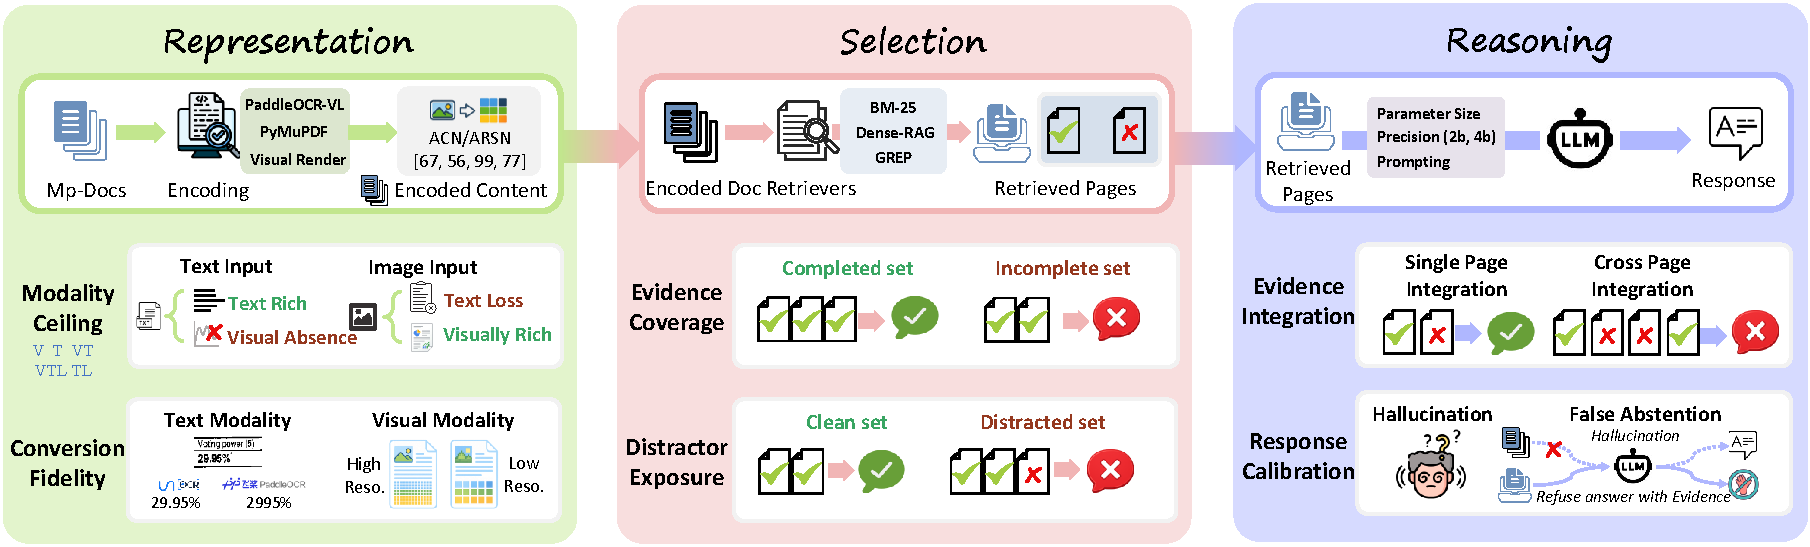
\includegraphics[width=\linewidth]{empirical/framework.pdf}
\caption{The three failure loci and their mechanisms.}
\label{fig:framework}
\end{figure*}

\subsection{Representation}
\label{sec:fm_representation}

Representation converts the document into the artifact consumed by later stages. This may be an embedded text layer, parser markdown, a cropped visual region, a rendered page, or a combination of these. Operations performed by the backbone after this artifact is tokenised, such as projection, resampling, or compression, belong to the reasoning locus because they are properties of how the backbone processes its input rather than of document conversion. The chosen representation determines both which document signals can be preserved and the cost of producing them. Representation failure occurs through two mechanisms:
\textbf{(1) Modality Ceiling.} Each modality can preserve only the signals it is capable of expressing, at the granularity permitted by its representation. Text tokens, for example, cannot capture non-linguistic visual information, while visual tokens preserve fine-grained detail only when sufficient spatial resolution and token budget are available.
\textbf{(2) Conversion Fidelity.} Even when a modality can represent a signal, the conversion process may degrade or corrupt it. Conversion fidelity measures how accurately the resulting artifact preserves information that the modality could otherwise carry. A document parser may, for example, misread a numeric value and leave the downstream reasoner operating on an incorrect but seemingly reliable representation \citep{zhang2025ocr}.

\subsection{Selection}
\label{sec:fm_selection}

Selection determines which parts of the encoded document are placed before the reasoner. This operation becomes necessary in the multi-page setting when the full document cannot be processed within the available context. Similarity retrieval is one implementation, but structural navigation, adaptive reranking, and agentic inspection perform the same underlying function, potentially over several iterations (\S\ref{sec:tf-retrieval}, \S\ref{sec:tf-agentic}). Selection may also operate at different granularities. Most systems select whole pages, matching common benchmark annotations and late-interaction retrievers, although sections, tables, or cropped figures may instead serve as the selected unit. Selection failure occurs through two mechanisms:
\textbf{(1) Evidence Coverage.} Evidence coverage measures how much of the evidence required to answer a question is present in the selected context, \emph{i.e.}, the recall of the required evidence units. Omitting required evidence leaves the reasoner with an incomplete evidence set and therefore places an upper bound on downstream accuracy regardless of reasoning capability.
\textbf{(2) Distractor Exposure.} Selection may also introduce content that is irrelevant to the question. Distractor exposure measures the extent to which such content accompanies the required evidence. Unlike evidence omission, distractors do not make the evidence intrinsically insufficient, but they increase the burden on the reasoner to identify and use the relevant content.

\subsection{Reasoning}
\label{sec:fm_reasoning}

Reasoning produces an answer from the evidence delivered by the preceding stages. Once the representation preserves the evidence a question requires and selection places that evidence before the reasoner, remaining failures are attributable to how the reasoner processes and acts on it. Such failures may be addressed through instruction, model scale, architecture, or training (\S\ref{sec:tf-reasoning}, \S\ref{sec:train-reasoning}). Reasoning can fail in many ways, including arithmetic errors over correctly read values or answering a different question from the one asked. We focus on two mechanisms that are particularly important in the multi-page setting:
\textbf{(1) Evidence Integration.} Multi-page questions may require complementary information distributed across several pages, including content whose meaning spans page boundaries. A reasoner may handle each piece of evidence correctly in isolation yet fail to connect them into the answer the question requires. This difficulty may be amplified in long contexts, where evidence at different positions is not used equally reliably \citep{liu2024lost}.
\textbf{(2) Response Calibration.} Response calibration concerns whether the model's answer reflects the level of support provided by the available evidence. Unlike integration, it can be tested both when sufficient evidence is present and when it is absent by construction. Failure occurs in two directions: \emph{hallucination}, where the model answers without sufficient supporting evidence \citep{li2023survey}, and \emph{false abstention}, where it refuses despite having sufficient evidence. We treat these as opposing outcomes of the same decision because interventions that make a model more willing to answer can reduce false abstention while increasing unsupported answers, and vice versa \citep{whitehead2022reliable}.

\section{Experimental Setup}
\label{sec:emp_experiments}
We instantiate the framework in a \textbf{single-pass retriever--generator} document question answering system, evaluated over two MP-VRDU benchmarks whose annotations make the controlled experiments possible. In this section, we first describe the system and the attribution experiments that isolate each mechanism (\S\ref{sec:attribution}), followed by the experimental configurations of representation, selection, and reasoning (\S\ref{sec:emp_representation}--\S\ref{sec:emp_reasoning}), including additional experiments comparing practical pipeline choices (\S\ref{sec:emp_additional}). 

\subsection{Attribution by Construction}
\label{sec:attribution}

The document question answering system consists of three stages that correspond to the three failure loci described in \S\ref{sec:attribution_framework}. For each question, the system performs the following:

\begin{enumerate}
\item \textbf{Encoding Stage:} each page is converted into the representation consumed by later stages, using parser markdown, a rendered page image, or both.
\item \textbf{Retrieval Stage:} a retriever scores every encoded page against the question and returns the highest-ranked $k$ pages. Retrieval operates at page granularity, matching the evidence annotations used by both benchmarks.
\item \textbf{Inference Stage:} a multimodal LLM receives the selected pages, the question, and a task instruction, then produces an answer in a single pass. The model has access only to the evidence delivered by the retrieval stage.
\end{enumerate}

The system's stages act once and in order, allowing failures to be attributed by constructing conditions that isolate one locus while holding the others fixed. Across the six mechanisms defined in \S\ref{sec:attribution_framework}, we vary the relevant representation, evidence, or reasoning condition and compare relevant metrics against an appropriate controlled baseline. Table~\ref{tab:experiments} summarises these experiments.

\begin{table}[h]
\centering
\small
\setlength{\tabcolsep}{4pt}
\renewcommand{\arraystretch}{1.15}
\begin{tabularx}{\linewidth}{@{}
  >{\raggedright\arraybackslash}p{2.3cm}
  l
  >{\raggedright\arraybackslash}X
  >{\raggedright\arraybackslash}X@{}}
\toprule
Locus & Mechanism & Constructed condition & Held fixed \\
\midrule
\multirow{3}{2.3cm}{\textbf{Representation}\\(Encoding stage: \S\ref{sec:emp_representation})}
 & Modality ceiling & Encoding rung compared across T, TL, TLV, V by evidence source & Gold pages, reasoner, prompt \\
\cmidrule(l){2-4}
 & Conversion fidelity & Text and image fidelity across three parsers and three render resolutions & Encoding rung, gold pages, reasoner, prompt \\
\midrule
\multirow{3}{2.3cm}{\textbf{Selection}\\(Retrieval stage: \S\ref{sec:emp_selection})}
 & Evidence coverage & Gold pages withheld from multi-page questions & Encoding, reasoner, prompt \\
\cmidrule(l){2-4}
 & Distractor exposure & Non-gold pages added at a fixed gold-page count & Gold set, encoding, reasoner, prompt \\
\midrule
\multirow{3}{2.3cm}{\textbf{Reasoning}\\(Inference stage: \S\ref{sec:emp_reasoning})}
 & Evidence integration & Evidence conditions requiring cross-page integration & Documents, gold pages, encoding \\
\cmidrule(l){2-4}
 & Response calibration & Answerable and unsupported evidence conditions & Gold pages, encoding, reasoner \\
\bottomrule
\end{tabularx}
\caption{Attribution by construction: conditions used to isolate failures.}
\label{tab:experiments}
\end{table}

\paragraph{Default Configuration.} Unless otherwise stated, pages are encoded at \textbf{TLV} using PaddleOCR-VL parser output and the \texttt{med} image preset, retrieved by ColQwen3, and passed to Qwen3-VL-8B-Instruct in \texttt{bf16}. Inference uses the prompt template in Figure~\ref{fig:prompt_template}, with selected pages ordered by their original document position. Generation is greedy (\texttt{do\_sample=False}) with no temperature, top-$p$, top-$k$, or repetition penalty. The default output limit is 256 tokens. Each experiment below changes only the representation, evidence set, or reasoning instruction required for the mechanism being tested.

\begin{figure}[h]
\centering
\begin{tcolorbox}[colback=gray!5,colframe=gray!50,boxrule=0.4pt,fontupper=\small\ttfamily,left=6pt,right=6pt]
You are answering a question about a document.\\[0.4em]
\{instruction\}\\[0.4em]
Question:\\
\{question\}\\[0.4em]
Document evidence:\\
\{context\}\\[0.4em]
Answer:
\end{tcolorbox}
\caption{Reasoner prompt template. \texttt{\{instruction\}} is empty in the default configuration. \texttt{\{context\}} is the selected pages in document order, as parser markdown, page images, or both according to the rung.}
\label{fig:prompt_template}
\end{figure}


\subsection{Representation Experiments}
\label{sec:emp_representation}

Each page is encoded from two signals: a text channel and a visual channel. The representation experiments run only on questions answerable from their annotated evidence, and modality comparisons are analysed according to the type of evidence source the question requires.

\paragraph{Modality ceiling.} We vary which signals reach the reasoner at all, across the four rungs of Table~\ref{tab:ladder_def}: embedded text (\textbf{T}), layout-aware parser text (\textbf{TL}), parser text combined with the page image (\textbf{TLV}), and the page image alone (\textbf{V}). The comparison tests whether the required evidence remains recoverable when textual, structural, or visual signals are unavailable, rather than assuming that one representation is uniformly preferable across question types.

\begin{table}[h]
\centering
\small
\setlength{\tabcolsep}{4pt}
\renewcommand{\arraystretch}{1.15}
\begin{tabularx}{\linewidth}{@{}
  >{\raggedright\arraybackslash}p{1.1cm}
  >{\raggedright\arraybackslash}p{3.2cm}
  >{\raggedright\arraybackslash}p{1.8cm}
  >{\raggedright\arraybackslash}p{2.6cm}
  >{\raggedright\arraybackslash}X@{}}
\toprule
Rep. & Text channel & Image & Cost & Role \\
\midrule
T   & Embedded text (PyMuPDF) & -- & Extraction only & Text floor; empty on scanned pages \\
TL  & Parser markdown & -- & Parser pass & Text-only ceiling; recovers reading order and table structure \\
TV  & Embedded text (PyMuPDF) & Page image & Extraction + vision tokens & Parser-free contrast to TLV \\
TLV & Parser markdown & Page image & Parser pass + vision tokens & Combined encoding; default \\
V   & -- & Page image & Vision tokens & Vision only \\
\bottomrule
\end{tabularx}
\caption{Representation ladder. Ordered by fidelity and, as a consequence, by cost.}
\label{tab:ladder_def}
\end{table}


\paragraph{Conversion fidelity.} We vary the quality of each channel while holding the representation rung fixed, through the parser for text and the render resolution for the image (Table~\ref{tab:fidelity}). These experiments test whether information that a modality can in principle represent is degraded before reaching the reasoner, and whether improving the fidelity of that conversion improves downstream performance.

\begin{table}[h]
\centering
\small
\setlength{\tabcolsep}{5pt}
\renewcommand{\arraystretch}{1.15}
\begin{tabular}{@{}lrl@{\hskip 1.2em\vrule\hskip 1.2em}lrrl@{}}
\toprule
\multicolumn{3}{@{}l}{\textit{Parser} (text channel)} & \multicolumn{4}{l@{}}{\textit{Resolution} (image channel)} \\
\cmidrule(r){1-3} \cmidrule(l){4-7}
Parser & Params & Rungs & Preset & Tok./page & Pixel cap & Rungs \\
\cmidrule(r){1-3} \cmidrule(l){4-7}
PaddleOCR-VL & 0.9B & TL, TLV & low & 285 & 313,600 & TLV, V \\
\cmidrule(r){1-3} \cmidrule(l){4-7}
MinerU 2.5 & 1.2B & TL, TLV & med & 456 & 501,760 & TLV, V \\
\cmidrule(r){1-3} \cmidrule(l){4-7}
Unlimited-OCR & 3.3B & TL, TLV & high & 744 & 752,640 & TLV, V \\
\bottomrule
\end{tabular}
\caption{Representation fidelity variation. PaddleOCR-VL and \texttt{med} are the defaults; the two halves vary independently. Tokens are Qwen3-VL's median visual tokens per page (one token per 32$\times$32\,px).}
\label{tab:fidelity}
\end{table}

\paragraph{Configuration.} All representation experiments use the dataset's annotated gold pages as an \texttt{oracle} evidence set, removing retrieval error from the comparison. The \textbf{T} rung supplies the PDF's embedded text layer directly through PyMuPDF, while \textbf{TL} supplies markdown produced by a layout-aware parser. \textbf{TLV} combines this markdown with the rendered page image, and \textbf{V} supplies the image alone; no bounding boxes or other explicit layout signals are passed to the reasoner. A fifth encoding, \textbf{TV}, combines embedded text with the page image without parsing and is used as a direct contrast against \textbf{TLV}. The default parser is PaddleOCR-VL (0.9B)~\citep{cui2025paddleocr}, with MinerU 2.5 (1.2B)~\citep{niu2026mineru2} and Unlimited-OCR (3.3B)~\citep{yin2026unlimited} used in the parser comparison. Pages are rasterised at 200 DPI and downsampled to the active image preset before inference. All experiments use \texttt{med} except the resolution sweep, which evaluates all three presets.

\subsection{Selection Experiments}
\label{sec:emp_selection}
Selection determines which evidence reaches the reasoner. We investigate failures caused by incomplete evidence coverage and by exposure to irrelevant pages.

\paragraph{Evidence coverage.} We vary how much of the required evidence reaches the reasoner by withholding gold pages from questions that cite more than one. These conditions run on multi-page questions only and are evaluated against the corresponding complete gold-page oracle. Pages are ranked by ColQwen3 within the document, allowing us to remove either the highest- or lowest-ranked gold page, or retain only one of them. A condition that a question cannot satisfy is excluded and recorded rather than silently satisfied with a different page set.

\paragraph{Distractor exposure.} We vary how much irrelevant evidence accompanies the required evidence by adding top-ranked non-gold pages to a complete gold set. Conditions are blocked on the exact gold-page count, so questions requiring different amounts of evidence are not pooled at the same retrieval depth. The range of $k$ narrows as the gold count rises, keeping the supplied context at six pages or fewer and preventing distractor count from being confounded with arbitrary increases in context length.

\begin{table}[h]
\centering
\small
\setlength{\tabcolsep}{5pt}
\renewcommand{\arraystretch}{1.15}
\begin{tabularx}{\linewidth}{@{}>{\raggedright\arraybackslash}p{2.4cm}>{\raggedright\arraybackslash}X>{\raggedright\arraybackslash}p{3.0cm}@{}}
\toprule
Condition & Pages supplied & Question pool \\
\midrule
\texttt{drop\_top}    & All gold pages except the highest-ranked & $\geq 2$ gold pages \\
\texttt{drop\_bottom} & All gold pages except the lowest-ranked  & $\geq 2$ gold pages \\
\texttt{keep\_top}    & The highest-ranked gold page only        & $\geq 2$ gold pages \\
\texttt{keep\_bottom} & The lowest-ranked gold page only         & $\geq 2$ gold pages \\
\midrule
$+k$ distractors & All gold pages plus the $k$ highest-ranked non-gold pages, $k \in \{3,5,7,10,13,15,18\}$ & Single-hop; multi-hop \\
\bottomrule
\end{tabularx}
\caption{Gold-set perturbations for the selection experiments, each compared with the complete gold set on the same questions.}
\label{tab:page_set}
\end{table}

\paragraph{Configuration.} ColQwen3 is used only to order pages within the constructed selection conditions. For evidence coverage, it ranks the annotated gold pages so that the highest- or lowest-ranked evidence can be removed or retained. For distractor exposure, non-gold pages are ranked separately and the highest-scoring distractors are appended to the complete gold set. Each constructed page set is then evaluated under \textbf{TLV}, and \textbf{V} representations. Verdict transitions are additionally measured against the corresponding complete-evidence \textbf{TLV} condition.

\subsection{Reasoning Experiments}
\label{sec:emp_reasoning}

Reasoning determines how the available evidence is used to produce a response. We investigate whether the reasoner can integrate complementary evidence across the supplied context and whether it can judge when that evidence is sufficient to support an answer.

\paragraph{Evidence integration.} We test evidence integration on answerable questions by supplying the annotated evidence pages directly and separating questions according to the structure of the evidence required to answer them. We first compare single-hop and multi-hop questions under the default \texttt{none} prompt to measure the integration deficit that remains once representation and selection are controlled. We then compare \texttt{none} against \texttt{cot} on the same evidence and question pools, testing whether explicit intermediate reasoning can recover performance specifically when evidence must be combined across pages.

\paragraph{Response calibration.} We test response calibration by varying both whether the supplied evidence supports an answer and whether the reasoner is explicitly instructed to abstain. The comparison uses the \texttt{none} and \texttt{abstain} prompts on answerable and unanswerable questions. Answerable questions receive their annotated gold pages, while unanswerable questions receive the top three pages ranked by BM25, providing plausible but non-supporting evidence. This allows us to measure unsupported answers when evidence is insufficient and false abstentions when it is sufficient.

\begin{table}[h]
\centering
\small
\begin{tabular}{lp{0.68\textwidth}}
\toprule
Mode & Instruction \\
\midrule
\texttt{none} & (empty) \\
\texttt{grounded} & Use only the provided document evidence and keep the answer concise. \\
\texttt{abstain} & \texttt{grounded}, plus: If the evidence does not contain the answer, answer exactly: Not answerable. \\
\texttt{abstain\_balanced} & \texttt{abstain}, plus: If the evidence does contain the answer, give it: do not decline a question the evidence supports. \\
\texttt{cot} & \texttt{grounded}, plus: Think step by step before answering. Then write your final answer on a new line beginning with `Answer:'. \\
\texttt{extract\_cot} & \texttt{grounded}, plus a verbatim-evidence extraction step, with visual evidence described in enough detail to answer from the description alone, then reasoning constrained to what was extracted, then the \texttt{Answer:} line. \\
\texttt{abstain\_cot} & \texttt{abstain}, plus: Think step by step before answering. Then write your final answer on a new line beginning with `Answer:'. \\
\bottomrule
\end{tabular}
\caption{Reasoning prompt modes for the \texttt{\{instruction\}} field. The main experiments use \texttt{none}, \texttt{cot}, \texttt{abstain}, and \texttt{abstain\_cot}; the remaining modes are reported in \S\ref{sec:emp_additional}.}
\label{tab:prompt_modes}
\end{table}

\paragraph{Configuration.} The three reasoning conditions differ only in the instruction inserted into Figure~\ref{fig:prompt_template}. Under \texttt{none}, the instruction field is empty. The \texttt{cot} condition instructs the model to reason through the supplied evidence before producing its answer, while \texttt{abstain} constrains the answer to the supplied evidence and permits \emph{Not answerable} when the required support is absent. Evidence pages are presented in document order under the active representation. The default 256-token output budget is retained for \texttt{none} and \texttt{abstain}, while \texttt{cot} allows up to 2048 tokens for intermediate reasoning.

\subsection{Additional Experiments}
\label{sec:emp_additional}

The attribution experiments above isolate the mechanisms that constrain MP-VRDU performance. We additionally examine practical implementation choices that affect how these findings translate into system design and deployment, focusing on retrieval strategy, prompting, and model configuration.

\paragraph{Retrievers.} We compare six page-level retrievers spanning lexical, dense-text, and late-interaction visual retrieval. Text retrievers consist of BM25, BGE-M3, and Qwen3-Embedding, while the vision retrievers consist of ColModernVBERT, ColQwen2.5, and ColQwen3. We additionally evaluate joint retrieval by taking the deduplicated union of matched text and vision retrievers. Retrieval is evaluated independently of answer generation using page-level precision, recall, and F1 against the annotated evidence pages across increasing retrieval depths. This characterises the practical trade-off between retrieval precision and evidence coverage when choosing how much and what kind of retrieval machinery to deploy.

\begin{table}[h]
\centering
\small
\setlength{\tabcolsep}{4pt}
\renewcommand{\arraystretch}{1.15}
\begin{tabularx}{\linewidth}{@{}
  >{\raggedright\arraybackslash}p{1.4cm}
  >{\raggedright\arraybackslash}p{3.4cm}
  >{\raggedright\arraybackslash}p{1.5cm}
  >{\raggedright\arraybackslash}X@{}}
\toprule
Arm & Retriever & Params & Index and cost \\
\midrule
Text & BM25 & -- & Term postings per document; no encoding pass \\
\midrule
Text & BGE-M3 & 568M & One vector per page \\
\midrule
Text & Qwen3-Embedding-4B & 4B & One vector per page; sequence cap 4096 \\
\midrule
Vision & ColModernVBERT & 250M & One vector per image patch; requires rendering \\
\midrule
Vision & ColQwen2.5 & 3B & One vector per image patch; requires rendering \\
\midrule
Vision & ColQwen3 & 4B & One vector per image patch; requires rendering \\
\bottomrule
\end{tabularx}
\caption{Selection: retriever exerpiments. Rrdered by cost within each arm. Late-interaction scoring stores many vectors per page rather than one, so the vision arm carries a larger index and a more expensive scoring pass than its parameter count alone suggests.}
\label{tab:retrievers}
\end{table}


\paragraph{Prompt modes.} Beyond the \texttt{none}, \texttt{cot}, and \texttt{abstain} conditions used in the main reasoning experiments, we evaluate the remaining prompt interventions in Table~\ref{tab:prompt_modes}. These vary how strongly the reasoner is grounded in the supplied context, how abstention is framed, and whether evidence is explicitly extracted before answering, while holding the supplied evidence fixed. This tests how far reasoning behaviour can be improved through inexpensive inference-time changes before altering the model or evidence pipeline.

\begin{table}[h]
\centering
\small
\begin{tabular}{ll}
\toprule
Axis & Checkpoints \\
\midrule
Scale & Qwen3-VL-Instruct at 2B, 4B, 8B, 32B; Gemma-3-IT at 4B, 12B, 27B \\
Precision & Qwen3-VL-8B at \texttt{bf16}, 8-bit, 4-bit; Qwen3-VL-32B at 4-bit \\
Family & InternVL3-8B, GLM-4.6V-Flash, MiniCPM-V-4.5, Llama-3.2-11B-Vision \\
Reasoning variant & Qwen3-VL-8B-Thinking \\
\bottomrule
\end{tabular}
\caption{Reasoner variations. All share the prompt template and decoding configuration of the default pipeline.}
\label{tab:reasoners}
\end{table}

\paragraph{Model variations.} We vary the reasoner across model scale, weight precision, and model family. Within Qwen3-VL, we compare models from 2B to 32B parameters, alongside 16-bit, 8-bit, and 4-bit variants of the 8B model. We additionally compare a quantised larger model against the full-precision 8B configuration at a similar memory budget, and compare Qwen3-VL-8B with alternative model families at approximately the same scale. These experiments directly examine the accuracy--resource trade-offs involved in selecting a reasoner for deployment.

\paragraph{Configuration.} The additional experiments inherit the default pipeline unless the component under study is explicitly varied. For retrieval, text models index both embedded PDF text and default-parser output, while visual retrievers operate on pages rendered at 200 DPI. Prompt and model comparisons use the same supplied evidence for each paired condition. Prompt modes requiring intermediate reasoning, and thinking-model variants, receive a 2048-token generation budget and mark the final response with \texttt{Answer:}, from which the answer is extracted before evaluation.

\section{Datasets and Evaluation}
\label{sec:dataset_evaluation}

In this section we describe the two datasets used for our experiments (\S\ref{sec:emp_mmlongbench}, \S\ref{sec:emp_longdocurl}) and conclude with the evaluation protocol (\S\ref{sec:emp_evaluation}).

\subsection{MMLongBench-Doc Dataset}
\label{sec:emp_mmlongbench}

MMLongBench-Doc~\citep{ma2024mmlongbench} is the primary dataset. It is the only multi-page benchmark we are aware of that annotates, per question, the evidence pages, the kind of evidence the question draws on, and the document's domain, while also supplying a pool of plausible questions unsupported by the document. Evidence pages make coverage measurable and define the oracle retriever, evidence source resolves representation findings by what the question actually requires, and the unanswerable pool makes calibration testable rather than inferred. The benchmark contains 135 documents averaging 47.5 pages and 847 answerable questions. Its questions are manually created or revised by expert annotators and subsequently quality-controlled. Multi-page questions are constructed to require information collection and reasoning over the annotated evidence pages, so we generally treat each gold page as necessary evidence rather than as another occurrence of the same answer. As with any human annotation, however, the page sets should not be assumed perfectly minimal in every case. Tables~\ref{tab:mmlb_composition} and \ref{tab:mmlb_labels} gives the composition.

\begin{table}[h]
\centering
\small
\begin{tabular}{lr@{\hskip 2em}lrrrr}
\toprule
Property & Value & Domain & Q & Docs & Digital & Scanned \\
\midrule
Questions        & 1,091 & Research report / Intro & 293 & 34 & 23 & 11 \\
Answerable       & 847   & Academic paper          & 204 & 26 & 26 & 0 \\
Unanswerable     & 244   & Guidebook               & 156 & 22 & 20 & 2 \\
Documents        & 135   & Tutorial / Workshop     & 139 & 17 & 3  & 14 \\
Mean pages/doc   & 48.3  & Financial report        & 117 & 11 & 11 & 0 \\
Median pages/doc & 28    & Brochure                & 101 & 15 & 13 & 2 \\
Pages min--max   & 9--468 & Admin / Industry       & 81  & 10 & 8  & 2 \\
\midrule
                 &       & \textbf{Total}          & \textbf{1,091} & \textbf{135} & \textbf{104} & \textbf{31} \\
\bottomrule
\end{tabular}
\caption{MMLongBench-Doc composition. Digital and scanned counts are documents, not questions.}
\label{tab:mmlb_composition}
\end{table}
\begin{table}[h]
\centering
\small
\begin{tabular}{lr@{\hskip 2em}lr@{\hskip 2em}lr}
\toprule
Evidence source & Q & Gold pages & Q & Answer format & Q \\
\midrule
Pure-text (plain)   & 298 & 1 page  & 485 & Int   & 290 \\
Figure              & 293 & 2 pages & 247 & Str   & 250 \\
Table               & 218 & 3+ pages & 113 & None  & 244 \\
Chart               & 178 & 0 pages & 246 & Float & 160 \\
Generalized-text (layout) & 119 & & & List & 147 \\
(none)              & 254 & & & & \\
\bottomrule
\end{tabular}
\caption{MMLongBench-Doc question labels. Evidence source is multi-label, so its column sums past the question count; the remaining columns are exclusive. Questions with three or more gold pages reach 24 at the tail.}
\label{tab:mmlb_labels}
\end{table}

\paragraph{Operational definitions.} Four labels are derived rather than read from the annotation, and each is fixed for every experiment.

\begin{enumerate}
    \item \textbf{Unanswerable} is a gold answer of exactly \emph{Not answerable}, giving 244 questions. A further two questions carry an answer with no annotated evidence page; they are excluded from the oracle conditions, which have no pages to supply.
    \item \textbf{Evidence pages} are converted from the dataset's 1-based numbering to 0-based indices, de-duplicated, and read as physical page positions, which is the dataset's own convention.
    \item \textbf{Scan status} is auto-detected per document. A page counts as carrying text when at least 20 characters are extractable, and a document is scanned when none of its sampled pages does. This gives 104 born-digital and 31 scanned documents.
    \item \textbf{Gold-page count} is the length of the de-duplicated evidence-page list, and is the hop label throughout: single-page questions cite one page, multi-page questions cite two or more.
\end{enumerate}

% \paragraph{Document domains.} MMLongBench-Doc assigns each document one of seven domains, manually categorised at collection~\citep{ma2024mmlongbench}. They are not defined in the source, so we characterise them by the documents they contain.

% \begin{itemize}
%     \item \textbf{Research report / Introduction:} survey and market-research reports, typically dense with charts and summary statistics.
%     \item \textbf{Academic paper:} conference and journal papers, with equations, figures, and reference lists.
%     \item \textbf{Guidebook:} product manuals and institutional handbooks, dominated by procedural text and inline icons.
%     \item \textbf{Tutorial / Workshop:} presentation decks, sparse in text per page and heavy in layout, and the domain with the most scanned documents.
%     \item \textbf{Financial report:} annual filings, whose content sits almost entirely in tables and running text.
%     \item \textbf{Brochure:} promotional and prospectus material, laid out for visual impact rather than reading order.
%     \item \textbf{Administration / Industry file:} internal and operational documents such as newsletters, forms, and industrial records.
% \end{itemize}

% \paragraph{Subsets.} The annotations determine which pool each experiment runs on. Representation and reasoning conditions use answerable questions, so accuracy is measured without abstention mixed into it. Coverage conditions withhold evidence from multi-page questions and are read against the multi-page oracle. Exposure conditions block on an exact gold-page count. Integration is analysed by both gold-page count and evidence-source count, separating questions that combine several sources on one page from those that combine evidence across pages. Multi-page questions range from two gold pages to a 24-page outlier, and 96 also cite more than one evidence source. Calibration pairs the answerable and unanswerable pools. Where informative, findings are additionally split by evidence source, document domain, and scan status.

\subsection{LongDocURL Dataset}
\label{sec:emp_longdocurl}

We additionally use LongDocURL~\citep{deng2025longdocurl} as a secondary dataset mainly for replication purposes. It contains 2,317 answerable questions over documents spanning 51--149 pages and provides task-family, question-type, answer-format, evidence-source, and evidence-page annotations. Its QA pairs and supporting evidence are produced through a semi-automated pipeline in which LLMs and LVLMs generate candidate questions and evidence before automated and human verification against the source document. Unlike MMLongBench-Doc, the annotated evidence pages are not a minimal set that must all be present to answer the question. Multiple annotated pages may contain redundant or independently sufficient evidence. We account for this distinction when interpreting LongDocURL coverage and integration results. Tables \ref{tab:ldu_composition} and \ref{tab:ldu_tasks} gives the composition.

\begin{table}[h]
\centering
\small
\begin{tabular}{lr@{\hskip 2em}lr@{\hskip 2em}lr}
\toprule
Property & Value & Evidence source & Q & Answer format & Q \\
\midrule
Questions        & 2,325   & Text   & 994 & String  & 941 \\
Documents        & 396     & Table  & 871 & List    & 757 \\
Mean pages/doc   & 85.6    & Layout & 779 & Integer & 431 \\
Median pages/doc & 78      & Figure & 548 & Float   & 185 \\
Pages min--max   & 51--149 & Others & 8   & None    & 11 \\
\bottomrule
\end{tabular}
\caption{LongDocURL composition. Evidence source is multi-label and sums past the question count; answer format is exclusive.}
\label{tab:ldu_composition}
\end{table}

\begin{table}[h]
\centering
\small
\begin{tabular}{llrrr}
\toprule
Task tag & Question type & Single-page & Multi-page & Total \\
\midrule
Understanding & extract          & 612 & 631 & 1,243 \\
\midrule
Locating & extract\_fig2tab      & 231 & 0   & 231 \\
         & topic2title           & 60  & 139 & 201 \\
         & summary2title         & 24  & 113 & 137 \\
         & summary2tab           & 8   & 118 & 126 \\
\midrule
Reasoning & calculate            & 89  & 56  & 145 \\
          & count                & 26  & 91  & 117 \\
          & compare              & 36  & 76  & 112 \\
          & summarize            & 7   & 6   & 13 \\
\midrule
\textbf{All} & & \textbf{1,093} & \textbf{1,230} & \textbf{2,325} \\
\bottomrule
\end{tabular}
\caption{LongDocURL question type by task tag and hop. Every type belongs to exactly one tag.}
\label{tab:ldu_tasks}
\end{table}

LongDocURL is less challenging than MMLongBench-Doc in several ways. Its documents are born-digital, it contains almost no unanswerable questions, and many questions can be answered directly from the document text, even when the annotated evidence is visual. We therefore use LongDocURL as a secondary dataset to test whether the main findings also hold under a less demanding setting.

% \paragraph{Operational definitions.} The derived labels follow Section~\ref{sec:emp_mmlongbench} except where the annotation differs.

% \begin{enumerate}
%     \item \textbf{Gold-page count} is the length of the evidence-page list, as before. Counting de-duplicated pages moves three questions from multi-page to single-page relative to the dataset's own totals, since three questions repeat a page. We report the dataset's totals so the figures are checkable against its paper, and run on the de-duplicated counts.
%     \item \textbf{Task tag} occupies the field the pipeline reads as the document label, so the Understanding, Locating, and Reasoning tags serve here as the stratification that document domain provides on MMLongBench-Doc.
%     \item \textbf{Unanswerable} questions number 8, which is too few to support a calibration condition.
% \end{enumerate}

\paragraph{Question types.} LongDocURL nests nine question types inside its three task tags~\citep{deng2025longdocurl}. Understanding and Reasoning are single types and four types respectively; the four Locating types are each defined by the pair of element types a question must move between.

\begin{itemize}
    \item \textbf{Understanding.} \texttt{extract} asks for information stated directly in the document, found by identifying keywords or reading a table.
    \item \textbf{Reasoning.} \texttt{calculate} requires arithmetic over extracted values; \texttt{count} requires enumerating instances; \texttt{compare} requires ordering or contrasting two or more values; \texttt{summarize} requires condensing content into a single statement.
    \item \textbf{Locating.} \texttt{topic2title} gives a description and asks which section title it matches; \texttt{summary2title} gives a paragraph summary and asks for the title of the section it came from; \texttt{summary2tab} gives a description and asks which named tables it refers to; \texttt{extract\_fig2tab} requires reading a figure and a table together to answer.
\end{itemize}

\subsection{Evaluation Protocol}
\label{sec:emp_evaluation}

\paragraph{Scoring and Judge Inputs.} Answers are scored by an LLM judge rather than exact match because correct responses may differ from the gold answer in units, rounding, or formatting. Each response is reduced to a binary \emph{correct}/\emph{incorrect} verdict based on semantic equivalence, and accuracy is the proportion judged correct. Gemini-2.5-Flash is the primary judge, run at temperature 0 with JSON-only output. Every judge receives the same four fields: the question, gold answer, an explicit unanswerable flag derived from the gold answer, and the model answer. The judge is not shown document content, evidence annotations, representation or retrieval settings, model configuration, prompt condition, or cost telemetry. This keeps the scoring criterion fixed across experimental arms and prevents the judge from conditioning on the manipulation being evaluated.

\begin{figure}[h]
\centering
\begin{tcolorbox}[colback=gray!5,colframe=gray!50,boxrule=0.4pt,fontupper=\small\ttfamily]
You judge answers to document questions.\\
Return only JSON with keys:\\
- verdict: one of correct, incorrect, abstained\\
- extracted\_answer: the answer extracted from the model response, or empty string\\
- rationale: a short reason\\[0.5em]
Mark correct when the model answer is semantically equivalent to the gold answer.\\
For unanswerable questions, mark correct only when the model abstains.\\[0.5em]
Return the verdict ``abstained'' whenever the response declines to answer because it judges the evidence insufficient, however it is worded. ``Not answerable'', ``the document does not provide this'', ``there is no document evidence to determine this'' and ``it is not possible to determine this from the given information'' are all abstentions. A response that notes a limitation and then commits to an answer anyway is NOT an abstention: judge the answer it commits to.
\end{tcolorbox}
\caption{Judge rubric.}
\label{fig:judge_prompt}
\end{figure}

\paragraph{Rubrics and Judge Validation.} Two judge rubrics are used over the same input payload. The \textit{accuracy rubric} in Figure~\ref{fig:judge_prompt} is used where only correctness is required, while the \textit{analysis rubric} in Figure~\ref{fig:judge_prompt_errcat} additionally supports abstention and error categorisation. Across 19,983 responses scored under both rubrics, the analysis rubric is 0.8--2.9 points stricter, but none of the 36 pairwise rung orderings reverses and key ladder deltas change by at most 0.8 points. We further validate the primary judge against GPT-4o, an independent model family, on 500 stratified responses, obtaining 96.0\% agreement and Cohen's $\kappa = 0.918$ (95\% CI [0.881, 0.951]). Against a human annotator on a 120-response subset, agreement is 98.3\% with $\kappa = 0.966$ (95\% CI [0.915, 1.000]). Agreement is stable across representation rungs (0.938--0.969), and the near-balanced validation pool yields a prevalence index of 0.156.
% and PABAK of 0.920.

% \paragraph{Error Categories.} Each incorrect response is assigned exactly one category from Table~\ref{tab:error_taxonomy}, using the listed priority order so that the first applicable category is selected. Correct responses receive no category. Because the analysis judge sees only the question, gold answer, unanswerable flag, and model answer, the taxonomy captures observable answer errors rather than inferred pipeline causes. It therefore cannot attribute failures to unseen factors such as a particular page, representation rung, retriever, or evidence source. The taxonomy is nearly exhaustive in practice, with \texttt{other} assigned to only one of the 1,853 incorrect responses on the representation ladder.

\begin{figure}[h]
\centering
\begin{tcolorbox}[colback=gray!5,colframe=gray!50,boxrule=0.4pt,fontupper=\small\ttfamily]
$\langle$accuracy only judge prompt, plus "abstained" in verdict choices$\rangle$
ABSTENTION\\
Return the verdict "abstained" whenever the response declines to answer because it judges the evidence insufficient, however it is worded. "Not answerable", "the document does not provide this", "there is no document evidence to determine this" and "it is not possible to determine this from the given information" are all abstentions. A response that notes a limitation and then commits to an answer anyway is NOT an abstention: judge the answer it commits to.\\[0.5em]
ERROR CATEGORY\\
Decide the verdict FIRST, using only the two rules above, and do not revisit it. The error category explains a verdict you have already reached; it never changes one. In particular, a response that states the gold answer in its own words, or surrounds it with explanation, is still correct.\\[0.5em]
$\langle$the eleven categories, in priority order$\rangle$
\end{tcolorbox}
\caption{Judge analysis rubric.}
% The correctness sentences are identical to Figure~\ref{fig:judge_prompt}; what is added is a definition of the \emph{abstained} verdict and the error taxonomy.}
\label{fig:judge_prompt_errcat}
\end{figure}
\begin{table}[h]
\centering
\small
\renewcommand{\arraystretch}{1.15}
\begin{tabular}{@{}ll@{}}
\toprule
\textbf{Category} & \textbf{Assigned when} \\
\midrule
\texttt{insufficient\_evidence} & The response declines: the evidence does not support an answer. \\
\texttt{no\_answer\_reached} & It reasons but never commits, trailing off or stopping mid-calculation. \\
\texttt{answered\_unanswerable} & The question is unanswerable and a substantive answer is given. \\
\texttt{equivocal} & The gold answer is present but not committed to. \\
\texttt{wrong\_count} & A "how many" question is answered with a different count. \\
\texttt{wrong\_value} & A non-count numeric answer differs from the gold value. \\
\texttt{wrong\_entity} & A non-numeric answer names a different thing. \\
\texttt{incomplete\_list} & The gold answer is a set and the response gives a subset. \\
\texttt{over\_inclusive\_list} & The response includes items the gold answer does not. \\
\texttt{unit\_or\_format\_mismatch} & The same quantity in a non-matching unit, scale or granularity. \\
\texttt{other} & None of the above. \\
\bottomrule
\end{tabular}
\caption{The error taxonomy in judge priority order.}
% The first category that fits an incorrect response is the one it receives, so the categories partition the incorrect responses in each condition.}
\label{tab:error_taxonomy}
\end{table}

\paragraph{Error categories.} Each incorrect response is assigned exactly one category from Table~\ref{tab:error_taxonomy}, using the listed priority order so that the first applicable category is selected. Categories are determined only from the question, gold answer, and model response; the judge is not shown the document pages, representation rung, or retriever, avoiding attribution to pipeline stages it cannot observe. Correct responses receive no category. The taxonomy is nearly exhaustive in practice, with \texttt{other} assigned to only one of the 1,853 incorrect responses on the representation ladder.

% \begin{enumerate}
%     \item \texttt{insufficient\_evidence}: The response declines because the evidence does not support an answer.
%     \item \texttt{no\_answer\_reached}: The response reasons but never commits, trailing off or stopping mid-calculation.
%     \item \texttt{answered\_unanswerable}: The question is unanswerable and a substantive answer is given.
%     \item \texttt{equivocal}: The gold answer is present but not committed to.
%     \item \texttt{wrong\_count}: A ``how many'' question is answered with a different count.
%     \item \texttt{wrong\_value}: A non-count numeric answer differs from the gold value.
%     \item \texttt{wrong\_entity}: A non-numeric answer names a different thing.
%     \item \texttt{incomplete\_list}: The gold answer is a set and the response gives a subset.
%     \item \texttt{over\_inclusive\_list}: The response includes items the gold answer does not.
%     \item \texttt{unit\_or\_format\_mismatch}: The same quantity is given in a non-matching unit, scale, or granularity.
%     \item \texttt{other}: None of the above.
% \end{enumerate}

% \paragraph{Confidence intervals.} Every reported accuracy carries a 95\% confidence interval from a document-level bootstrap: 1,000 resamples at a fixed seed, taking the 2.5 and 97.5 percentiles. Documents are resampled rather than questions, because questions drawn from one document are not independent and a question-level interval would understate the variation. Every reported condition runs over its whole pool rather than a sample, so no sampling stage enters the interval.

% \paragraph{Comparisons.} Two conditions are read as different when their intervals separate. Sufficiency comparisons, which ask whether a cheaper encoding matches a richer one rather than whether it differs from it, use a pre-registered margin of 3 accuracy points. Paired conditions over the same questions are additionally read as verdict transitions, reporting the proportion of oracle-correct answers a change breaks and the proportion of oracle-incorrect answers it repairs. A net difference alone cannot distinguish a condition that leaves answers untouched from one that breaks and repairs in equal measure, and the two carry different implications for what failed.

% \paragraph{Reproducibility.} Every condition is decoded greedily, with self-consistency the single exception, so a condition is reproducible from its identity. One result cell is identified by the question, the page set, the representation, the reasoner, the visual resolution, and the prompt mode. Cells are cached under that identity, so two conditions differing in any of it cannot collide, and every reported figure is traceable to the configuration that produced it.


\section{Empirical Findings}
\label{sec:emp_findings}

We organise the findings by where failures arise in the MP-VRDU pipeline. \S\ref{sec:findings_representation} examines representation, showing when information is lost through modality limits or imperfect conversion. \S\ref{sec:findings_selection} studies selection, where incomplete evidence coverage is substantially more damaging than moderate distractor exposure. \S\ref{sec:findings_reasoning} then examines reasoning, where the remaining bottlenecks are evidence integration and response calibration.

\subsection{Representation}
\label{sec:findings_representation}

Representation determines what evidence remains available for downstream reasoning. OCR-free approaches preserve visual and spatial signals that text extraction may discard \citep{cho2024m3docrag,tanaka2025vdocrag}, while text-based and joint representations can expose linguistic content more directly \citep{hannan2026docslm,han2025mdocagent,suri2025visdom}. Our results separate these effects into two mechanisms: \emph{modality ceiling}, which determines what information a representation can expose at all, and \emph{conversion fidelity}, which determines how much of that information survives encoding.

\subsubsection{Modality Ceiling}

% GENERATED by tables/scripts/ -- do not edit by hand, re-run the script.
% Numbers read from results/tables/analysis/*.csv.
% analysis/faithfulness_answerable_accuracy_source (results.errcat.jsonl)
% Shade ranges are fitted to the values present:
% Accuracy: accteal over [14.5, 51.0]  % Abstention: neutral over [0.8, 36.6]  % Incorrect (hallucinated): recwarm over [40.1, 56.7]
\definecolor{accteal}{HTML}{1BAF7A}
\definecolor{neutral}{HTML}{5B6B7F}
\definecolor{recwarm}{HTML}{D95926}
\begin{table}[ht]
\centering
\small
\setlength{\tabcolsep}{5pt}
\adjustbox{max width=\textwidth}{%
\begin{tabular}{l@{\hskip 14pt}rrrr@{\hskip 14pt}rrrr@{\hskip 14pt}rrrr}
\toprule
 & \multicolumn{4}{c}{\textbf{Accuracy}} & \multicolumn{4}{c}{\textbf{Abstention}} & \multicolumn{4}{c}{\textbf{Incorrect}} \\
\cmidrule(lr){2-5} \cmidrule(lr){6-9} \cmidrule(lr){10-13}
\textbf{Evidence source} & \textbf{T} & \textbf{TL} & \textbf{TLV} & \textbf{V} & \textbf{T} & \textbf{TL} & \textbf{TLV} & \textbf{V} & \textbf{T} & \textbf{TL} & \textbf{TLV} & \textbf{V} \\
\midrule
Text & \cellcolor{accteal!37}\textbf{36.9} & \cellcolor{accteal!49}44.4 & \cellcolor{accteal!60}\textbf{51.0} & \cellcolor{accteal!46}42.3 & \cellcolor{neutral!37}23.0 & \cellcolor{neutral!18}11.5 & \cellcolor{neutral!11}7.3 & \cellcolor{neutral!12}8.0 & \cellcolor{recwarm!0}40.1 & \cellcolor{recwarm!14}44.1 & \cellcolor{recwarm!5}41.6 & \cellcolor{recwarm!35}49.7 \\
Layout & \cellcolor{accteal!19}26.3 & \cellcolor{accteal!32}33.9 & \cellcolor{accteal!57}49.2 & \cellcolor{accteal!47}\textbf{43.2} & \cellcolor{neutral!33}20.3 & \cellcolor{neutral!16}10.2 & \cellcolor{neutral!0}\textbf{0.8} & \cellcolor{neutral!6}\textbf{4.2} & \cellcolor{recwarm!48}\textbf{53.4} & \cellcolor{recwarm!57}\textbf{55.9} & \cellcolor{recwarm!36}\textbf{50.0} & \cellcolor{recwarm!45}52.5 \\
Table & \cellcolor{accteal!35}35.6 & \cellcolor{accteal!50}\textbf{44.7} & \cellcolor{accteal!50}44.7 & \cellcolor{accteal!32}34.1 & \cellcolor{neutral!25}\textbf{15.9} & \cellcolor{neutral!11}\textbf{7.2} & \cellcolor{neutral!10}6.7 & \cellcolor{neutral!14}9.1 & \cellcolor{recwarm!31}48.6 & \cellcolor{recwarm!29}48.1 & \cellcolor{recwarm!31}48.6 & \cellcolor{recwarm!60}\textbf{56.7} \\
Chart & \cellcolor{accteal!3}16.3 & \cellcolor{accteal!4}16.9 & \cellcolor{accteal!46}42.7 & \cellcolor{accteal!43}40.4 & \cellcolor{neutral!53}32.6 & \cellcolor{neutral!46}28.1 & \cellcolor{neutral!11}7.3 & \cellcolor{neutral!9}6.2 & \cellcolor{recwarm!40}51.1 & \cellcolor{recwarm!54}55.1 & \cellcolor{recwarm!36}\textbf{50.0} & \cellcolor{recwarm!48}53.4 \\
Figure & \cellcolor{accteal!0}14.5 & \cellcolor{accteal!12}22.1 & \cellcolor{accteal!46}42.4 & \cellcolor{accteal!40}39.0 & \cellcolor{neutral!60}36.6 & \cellcolor{neutral!40}24.8 & \cellcolor{neutral!11}7.6 & \cellcolor{neutral!12}7.9 & \cellcolor{recwarm!32}49.0 & \cellcolor{recwarm!47}53.1 & \cellcolor{recwarm!36}\textbf{50.0} & \cellcolor{recwarm!47}53.1 \\
\emph{All} & \cellcolor{accteal!24}29.0 & \cellcolor{accteal!35}35.7 & \cellcolor{accteal!58}49.5 & \cellcolor{accteal!46}42.6 & \cellcolor{neutral!43}26.3 & \cellcolor{neutral!27}17.2 & \cellcolor{neutral!9}6.2 & \cellcolor{neutral!11}7.1 & \cellcolor{recwarm!17}44.7 & \cellcolor{recwarm!26}47.2 & \cellcolor{recwarm!15}44.3 & \cellcolor{recwarm!37}50.3 \\
\bottomrule
\end{tabular}%
}

\caption[Answer outcomes by evidence source]{Answer outcomes by evidence source and representation rung on MMLongBench-Doc. Richer representations primarily reduce abstention, while the incorrect rate remains broadly stable.}
\label{tab:ladder_source}
\end{table}
% {\footnotesize\raggedright
% Judge-scored rates (\%) on the answerable pool, oracle pages, under the error-taxonomy judge
% (the one that defines the abstained verdict), so levels here are not interchangeable with the
% tables scored by the main report's judge. The three blocks partition each cell's questions and
% sum to 100: a question is answered correctly, declined, or answered wrongly. Abstention counts
% refusals the judge did not credit, which is why the three close exactly where
% $100 - \text{accuracy} - \text{abstention}$ need not. Bold is the largest value per column,
% except abstention where it is the smallest; \emph{All} is excluded from that contest, since it
% pools the rows above it rather than competing with them. A question citing several sources
% counts under each, so the source rows overlap and do not sum to \emph{All}.
% \textbf{Abstention here is not purely an error}, which is why it carries no direction: at
% \textbf{T} a scanned page has no embedded text layer, so declining is correct for what that
% rung delivered, and the born-digital component of the source table is the false-abstention
% rate. \textbf{The incorrect block is the one that makes the ladder's case}: it is flat across
% the four rungs, so the accuracy the ladder buys comes out of abstention and not out of
% hallucination.\par}


\paragraph{Vision Is Necessary but Not Sufficient.} The representation ladder shows that vision expands what the system can answer, but does not replace explicit text. At \textbf{T} and \textbf{TL}, abstention is particularly high for chart questions (32.6\% and 28.1\%) and figure questions (36.6\% and 24.8\%), but falls to 7.3\% and 7.6\% at \textbf{TLV}. Since the annotated gold pages are supplied throughout, these refusals expose a modality ceiling: text-only representations often do not preserve the graphical or spatial signal required by the question. Vision alone is also weaker than the joint representation, with \textbf{V} reaching 42.6\% compared with 49.5\% for \textbf{TLV}. This does not imply that the visual input lacks the corresponding linguistic information; rather, fine-grained text may be difficult to recover at the available resolution and visual-token budget, whereas an explicit text channel exposes it directly. This complements the original MMLongBench-Doc observation that OCR-fed LLMs often outperform vision-language models \citep{ma2024mmlongbench}. The strongest representation is therefore multimodal because each channel compensates for information that is unavailable or difficult to access through the other.

\begin{figure}[ht]
\centering
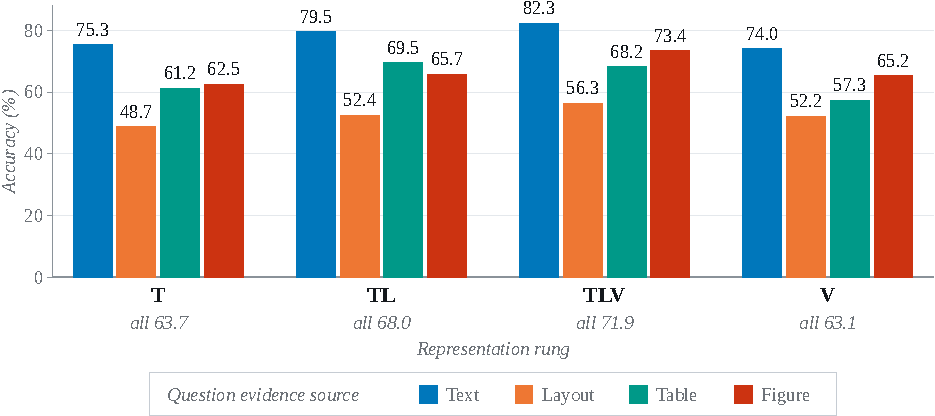
\includegraphics[width=0.8\columnwidth]{empirical/findings_figures/ladder_ldu_sources.pdf}
\caption[LongDocURL accuracy by representation rung and evidence source]{LongDocURL accuracy by representation rung and evidence source. Evidence-source differences remain substantial across representation rungs.}
\label{fig:ladder_ldu_sources}
\end{figure}

\paragraph{The Modality Ceiling Depends on the Document Distribution.} LongDocURL reproduces the overall advantage of \textbf{TLV}, but with a substantially weaker modality gap (Figure~\ref{fig:ladder_ldu_sources}). Its documents are born-digital and frequently expose answer-relevant content through the text layer even when the annotated evidence source is visual. Figure questions, for example, already reach 62.5\% at \textbf{T} and 65.7\% at \textbf{TL}, rising to 73.4\% at \textbf{TLV}. These easier documents reveal that modality ceiling is not determined by an evidence label alone: a question annotated to a figure may still be answerable through redundant surrounding text. Vision becomes most important when the required signal is genuinely absent from the textual representation, as occurs more often for charts, complex layouts, and scanned or visually dense documents. The value of a modality therefore depends on how much unique information it contributes within the target document distribution, rather than on a universal preference for text or vision.

\subsubsection{Conversion Fidelity}

\begin{figure}[ht]
\centering
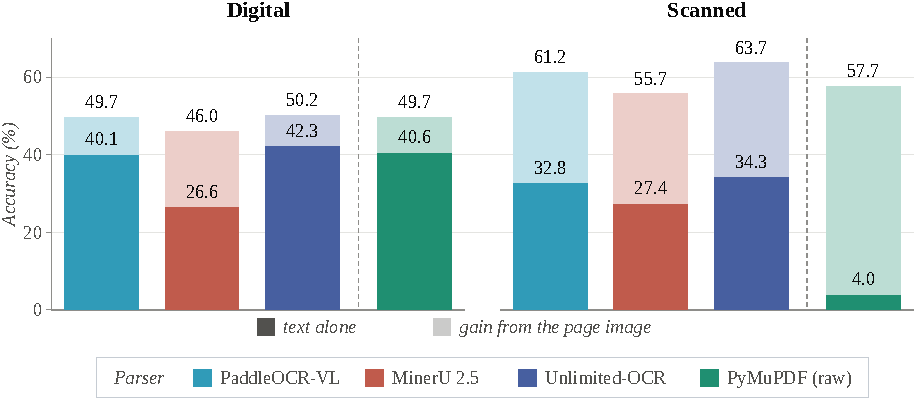
\includegraphics[width=0.7\columnwidth]{empirical/findings_figures/parser.pdf}
\caption[Parser accuracy by text source]{Parser accuracy by text source with and without page images. Adding vision substantially reduces sensitivity to parser choice, particularly on scanned documents.}
\label{fig:parser}
\end{figure}

\paragraph{Conversion Errors Matter Most Without a Redundant Channel.} Parser choice produces substantial differences when text must carry the evidence alone, confirming that conversion is not a neutral preprocessing step. MinerU reaches 26.6\% on born-digital and 27.4\% on scanned documents, compared with 40.1\% and 32.8\% for PaddleOCR-VL and 42.3\% and 34.3\% for Unlimited-OCR. The distinction between document types is important: on born-digital documents, parsing mainly restructures an existing text layer, whereas on scans it determines whether a usable text representation is recovered at all. PyMuPDF makes this extreme, falling to 4.0\% on scanned documents where an embedded text layer is often absent. These results corroborate prior findings that OCR and structural parsing errors propagate into downstream RAG performance \citep{zhang2025ocr,sun2026when}. Our multimodal conditions add a further qualification: once vision accompanies the parsed text, the spread between parsers contracts from 15.7 to 4.2 points on digital documents and from 30.3 to 8.0 on scans. Conversion errors are therefore most damaging when they destroy the only representation carrying the required signal; when another modality preserves the source information, downstream reasoning can often compensate.

% Resolution sweep by evidence source: low/med/high at the TLV and V rungs.
% Teal = accuracy on the shared ladder scale; warm = the low->high gain (points).
% Bold marks the best resolution in each row, within each rung block.
\definecolor{accteal}{HTML}{1BAF7A}
\definecolor{recwarm}{HTML}{D95926}
\newcommand{\rshade}[1]{%
  \pgfmathtruncatemacro{\shadeval}{max(0,min(60,(#1-14)/(74-14)*65))}%
  \edef\tmpcol{accteal!\shadeval}%
  \expandafter\cellcolor\expandafter{\tmpcol}%
}
\newcommand{\rcell}[1]{\rshade{#1}#1}
\newcommand{\rbest}[1]{\rshade{#1}\textbf{#1}}
\newcommand{\rgain}[1]{%
  \pgfmathtruncatemacro{\shadeval}{max(0,min(55,(#1-0)/(18-0)*55))}%
  \edef\tmpcol{recwarm!\shadeval}%
  \expandafter\cellcolor\expandafter{\tmpcol}$+$#1%
}

\begin{table}[ht]
\centering
\small
\setlength{\tabcolsep}{5pt}
\renewcommand{\arraystretch}{1.12}
\begin{tabular}{l rrrr @{\hskip 10pt\vrule\hskip 10pt} rrrr}
\toprule
 & \multicolumn{4}{c@{\hskip 10pt}}{\textbf{TLV}} & \multicolumn{4}{c}{\textbf{V}} \\
\cmidrule(r){2-5}\cmidrule(l){6-9}
Evidence source & low & med & high & $\Delta$ & low & med & high & $\Delta$ \\
\midrule
Chart            & \rcell{38.2} & \rcell{44.9} & \rbest{48.3} & \rgain{10.1} & \rcell{34.3} & \rcell{44.9} & \rbest{48.3} & \rgain{14.0} \\
Figure           & \rcell{39.7} & \rcell{45.5} & \rbest{48.3} & \rgain{8.6}  & \rcell{38.3} & \rcell{40.0} & \rbest{43.8} & \rgain{5.5} \\
Layout & \rcell{46.6} & \rcell{50.0} & \rbest{54.2} & \rgain{7.6}  & \rcell{47.5} & \rcell{49.2} & \rbest{53.4} & \rgain{5.9} \\
Text        & \rcell{52.9} & \rbest{55.0} & \rbest{55.0} & \rgain{2.1}  & \rcell{38.8} & \rcell{45.4} & \rbest{51.5} & \rgain{12.7} \\
Table            & \rcell{48.8} & \rbest{49.8} & \rcell{48.8} & \rgain{0.0}  & \rcell{25.3} & \rcell{37.3} & \rbest{42.4} & \rgain{17.1} \\
\midrule
\textbf{All}     & \rcell{49.2} & \rcell{52.5} & \rbest{54.7} & \rgain{5.5}  & \rcell{37.8} & \rcell{45.7} & \rbest{50.2} & \rgain{12.4} \\
\bottomrule
\end{tabular}
\caption{Render resolution by evidence source. On MMLongBench-Doc, at the TLV and V rungs. $\Delta$ indicates difference between high and low resolution.}
\label{tab:resolution_sweep}
\end{table}

\paragraph{Visual Fidelity Follows the Same Pattern.} Render resolution exposes the same mechanism from the visual side. Increasing resolution produces a much larger improvement for \textbf{V} than for \textbf{TLV}, where accompanying text already preserves part of the fine-grained information that additional pixels would recover (Table~\ref{tab:resolution_sweep}). This mirrors the motivation behind high-resolution compression methods such as mPLUG-DocOwl2, where preserving visual detail across many pages must be balanced against the resulting visual-token cost \citep{hu2025mplug}. Low-resolution rendering is therefore most restrictive when vision alone must carry small text, spatial detail, or other fine-grained evidence. Parser quality and render resolution expose the same underlying principle: conversion fidelity matters most when degradation removes the last usable copy of the information needed to answer.

\subsection{Selection}
\label{sec:findings_selection}

Selection determines which evidence reaches the reasoner. While both incomplete retrieval and irrelevant context can limit long-document understanding, our results show that their effects are asymmetric: missing required evidence removes information that downstream stages cannot recover, whereas moderate distractor exposure is often tolerated within the context range we test.

\subsubsection{Evidence Coverage}

\begin{figure}[h]
    \centering
    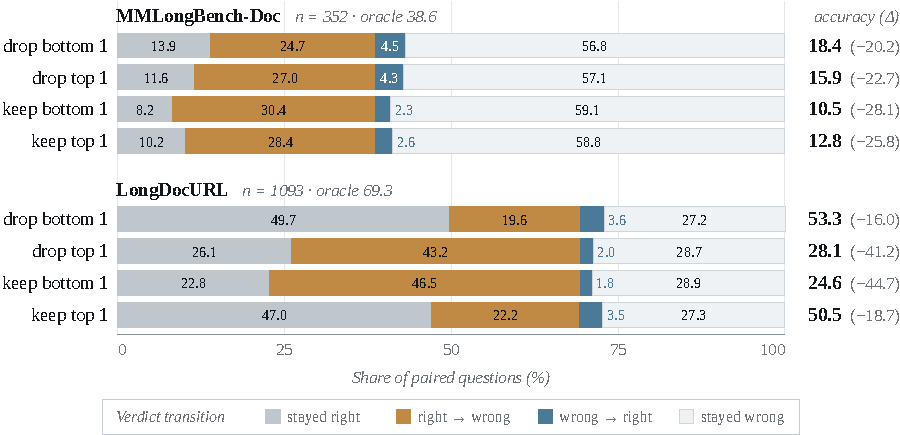
\includegraphics[width=0.9\columnwidth]{empirical/findings_figures/sufficiency.pdf}
    \caption[Verdict transitions under partial evidence coverage]{Verdict transitions after withholding or retaining gold evidence pages on MMLongBench-Doc and LongDocURL. Missing evidence predominantly converts correct answers into incorrect ones, while repairs are comparatively rare.}
    \label{fig:sufficiency}
\end{figure}

\paragraph{Evidence Coverage Is a Hard Constraint.} Removing required evidence overwhelmingly converts previously correct answers into incorrect ones, while the reverse transition is rare (Figure~\ref{fig:sufficiency}). On MMLongBench-Doc, withholding a single gold page breaks 24.7--27.0\% of previously correct answers, compared with only 4.3--4.5\% being repaired. Retaining just one gold page widens this imbalance further, with 28.4--30.4\% changing from correct to incorrect and only 2.3--2.6\% moving in the opposite direction. The result is therefore more than the expected correlation between retrieval recall and accuracy: directly removing known evidence produces a strongly directional loss that downstream reasoning rarely reverses. This complements retrieval-depth studies showing that broader retrieval initially improves performance as evidence recall rises \citep{jin2025long}, while isolating the mechanism responsible for that early gain.

\begin{figure}[!h]
  \centering
  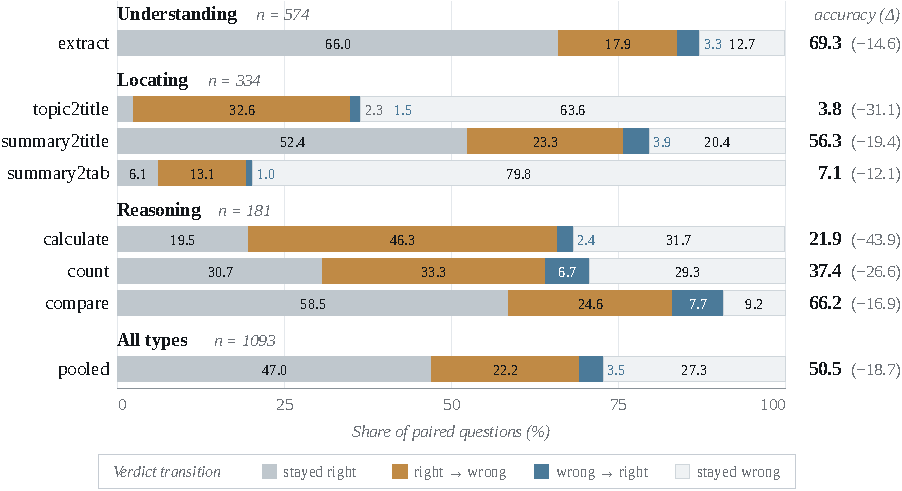
\includegraphics[width=0.9\columnwidth]{empirical/findings_figures/coverage_types.pdf}
  \caption[LongDocURL coverage sensitivity by question type]{LongDocURL verdict transitions under partial evidence coverage, grouped by question type. Extractive questions are relatively robust, while question types requiring evidence combination show substantially larger losses.}
  \label{fig:coverage_types}
\end{figure}


\paragraph{Evidence Importance Shapes Coverage Loss.} The effect of missing evidence also depends on which evidence survives. On LongDocURL, retaining only the highest-ranked gold page preserves substantially more performance than removing it, while dropping the lowest-ranked page is considerably less damaging. MMLongBench-Doc is less forgiving, consistent with its multi-page questions more often depending jointly on several pieces of evidence. Figure~\ref{fig:coverage_types} shows the same pattern by question type: \texttt{extract} questions are comparatively robust when only part of the annotated evidence remains, whereas \texttt{calculate}, \texttt{count}, and \texttt{topic2title} suffer much larger losses. Selection quality therefore depends not only on how much evidence is retrieved, but on whether the evidence most critical to the required operation is preserved.

\subsubsection{Distractor Exposure}

% Adding distractor pages to a complete gold set, both datasets, k up to 5.
% Shading matches the withholding table. Both emit these \providecommand macros,
% so either table can be \input alone or first, in any order.
% Transition rows in the two-gold block pool questions with two and three gold
% pages. Cells beyond three distractors ran at TLV only on MMLongBench-Doc, and
% accuracy at the deeper counts is read on a shrinking pool under OOM attrition;
% the paired transition columns are unaffected.
\definecolor{accteal}{HTML}{1BAF7A}
\definecolor{recwarm}{HTML}{D95926}
\providecommand{\mshade}[1]{%
  \pgfmathtruncatemacro{\shadeval}{max(0,min(60,(#1-8)/(70-8)*65))}%
  \edef\tmpcol{accteal!\shadeval}\expandafter\cellcolor\expandafter{\tmpcol}}
\providecommand{\mcell}[1]{\mshade{#1}#1}
\providecommand{\mbest}[1]{\mshade{#1}\textbf{#1}}
\providecommand{\lshade}[1]{%
  \pgfmathtruncatemacro{\shadeval}{max(0,min(60,(#1-20)/(80-20)*65))}%
  \edef\tmpcol{accteal!\shadeval}\expandafter\cellcolor\expandafter{\tmpcol}}
\providecommand{\lcell}[1]{\lshade{#1}#1}
\providecommand{\lbest}[1]{\lshade{#1}\textbf{#1}}
\providecommand{\dmg}[1]{%
  \pgfmathtruncatemacro{\shadeval}{max(0,min(55,(#1)/48*55))}%
  \edef\tmpcol{recwarm!\shadeval}\expandafter\cellcolor\expandafter{\tmpcol}#1}
\providecommand{\rep}[1]{%
  \pgfmathtruncatemacro{\shadeval}{max(0,min(55,(#1)/48*55))}%
  \edef\tmpcol{accteal!\shadeval}\expandafter\cellcolor\expandafter{\tmpcol}#1}

\begin{table}[!h]
\centering
\small
\setlength{\tabcolsep}{3pt}
\renewcommand{\arraystretch}{1.12}
\begin{tabular}{l rrrr rr @{\hskip 6pt\vrule\hskip 6pt} rrrr rr}
\toprule
 & \multicolumn{6}{c@{\hskip 6pt}}{\textbf{MMLongBench-Doc}} & \multicolumn{6}{c}{\textbf{LongDocURL}} \\
\cmidrule(r){2-7}\cmidrule(l){8-13}
Condition & T & TL & TLV & V & R$\rightarrow$W & W$\rightarrow$R & T & TL & TLV & V & R$\rightarrow$W & W$\rightarrow$R \\
\midrule
\multicolumn{13}{@{}l}{\emph{1 gold page}} \\
Oracle           & \mcell{37.1} & \mcell{44.6} & \mbest{63.7} & \mcell{55.0} & --- & --- & \lcell{65.6} & \lcell{74.0} & \lbest{74.7} & \lcell{64.5} & --- & --- \\
$+$1 distractor  & \mcell{39.5} & \mcell{48.9} & \mbest{63.7} & \mcell{55.7} & \dmg{7.8} & \rep{7.0} & \lcell{65.4} & \lcell{72.4} & \lbest{74.4} & \lcell{63.0} & \dmg{8.5} & \rep{8.1} \\
$+$2 distractors & \mcell{38.8} & \mcell{47.9} & \mbest{64.3} & \mcell{56.1} & \dmg{8.2} & \rep{8.0} & \lcell{65.1} & \lcell{68.7} & \lbest{72.0} & \lcell{63.9} & \dmg{9.3} & \rep{7.5} \\
$+$3 distractors & \mcell{40.9} & \mcell{47.0} & \mbest{63.1} & \mcell{55.1} & \dmg{9.7} & \rep{8.2} & \lcell{64.5} & \lcell{68.0} & \lbest{68.4} & \lcell{62.1} & \dmg{11.7} & \rep{6.9} \\
$+$4 distractors & \mcell{41.9} & \mcell{45.3} & \mbest{62.5} & \mcell{52.5} & \dmg{9.5} & \rep{6.6} & \lcell{63.5} & \lcell{68.0} & \lbest{72.2} & \lcell{62.5} & \dmg{10.5} & \rep{8.7} \\
$+$5 distractors & \mcell{39.5} & \mcell{42.6} & \mbest{62.3} & \mcell{54.4} & \dmg{10.0} & \rep{6.9} & \lcell{64.6} & \lcell{69.1} & \lbest{70.2} & \lcell{60.8} & \dmg{11.4} & \rep{7.3} \\
\addlinespace
\multicolumn{13}{@{}l}{\emph{2 gold pages}} \\
Oracle           & \mcell{28.9} & \mcell{33.3} & \mbest{37.8} & \mcell{34.6} & --- & --- & \lcell{62.2} & \lcell{63.4} & \lbest{70.4} & \lcell{61.5} & --- & --- \\
$+$1 distractor  & \mcell{25.7} & \mcell{34.0} & \mbest{38.6} & \mcell{34.4} & \dmg{7.8} & \rep{7.5} & \lcell{58.7} & \lcell{63.0} & \lbest{66.2} & \lcell{57.9} & \dmg{9.6} & \rep{4.1} \\
$+$2 distractors & \mcell{25.3} & \mcell{33.6} & \mbest{35.7} & \mcell{32.4} & \dmg{9.6} & \rep{6.0} & \lcell{58.9} & \lcell{62.2} & \lbest{66.4} & \lcell{57.4} & \dmg{10.9} & \rep{4.4} \\
$+$3 distractors & \mcell{21.6} & \mcell{28.2} & \mbest{33.6} & \mcell{33.2} & \dmg{11.4} & \rep{6.0} & \lcell{58.1} & \lcell{63.3} & \lbest{70.8} & \lcell{57.8} & \dmg{9.7} & \rep{6.0} \\
$+$4 distractors & \mcell{24.6} & \mcell{30.7} & \mbest{43.7} & \mcell{31.3} & \dmg{11.8} & \rep{11.8} & \lcell{57.8} & \lcell{63.2} & \lbest{68.3} & \lcell{57.1} & \dmg{13.3} & \rep{6.1} \\
% $+$5 distractors & \mcell{20.5} & \mcell{29.5} & \mbest{44.7} & \mcell{32.1} & \dmg{10.6} & \rep{8.2} & \lcell{56.4} & \lcell{61.5} & \lbest{69.0} & \lcell{54.9} & \dmg{12.6} & \rep{5.9} \\
\bottomrule
\end{tabular}
\caption{Adding distractor pages to a complete gold set. Distractors ranked by ColQwen3 and verdict transitions indicate the proportion of questions that turned incorrect when previously correct or vice versa when distractors were added at the \textbf{TLV} rung.}
\label{tab:exposure}
\end{table}

\paragraph{Distractor Exposure Produces Stable Accuracy with Mild Degradation.} Across both datasets, adding non-gold pages produces only modest changes in aggregate accuracy within the tested range. On MMLongBench-Doc, performance remains broadly stable for single-page questions and declines gradually for multi-page questions as additional pages are introduced, while LongDocURL shows even less degradation under comparable distractor counts. This pattern is consistent with prior work showing that distractor effects are not monotonic or uniform: Cuconasu et al. find that their impact depends strongly on semantic relatedness and position \citep{cuconasu2024power}, while Jin et al. report a rise-then-fall relationship in which increasing retrieval depth initially improves performance before accumulated hard negatives begin to reduce it \citep{jin2025long}. The apparent stability in our results therefore should not be interpreted as evidence that added pages are harmless; instead, it suggests that positive and negative effects can partially cancel at the aggregate level, motivating a closer examination of the underlying verdict transitions.

\paragraph{Non-Gold Pages Can Both Distort and Complete the Evidence.} The verdict transitions refine this picture. Cuconasu et al. show that additional context can help or hurt depending on its relevance and position \citep{cuconasu2024power}, while Jin et al. show that hard negatives can mislead the reasoner even when relevant evidence is already present \citep{jin2025long}. Manual inspection of our transitions reveals a related document-specific effect: non-gold pages can contain contextual information that changes how the annotated evidence should be interpreted. In right-to-wrong cases, added pages sometimes introduce partial evidence that leads the reasoner to overcount or misinterpret the gold pages; in wrong-to-right cases, they can provide disambiguating or supplementary context that repairs an otherwise incorrect answer. Retrieval depth therefore trades not only noise against coverage, but also incomplete against more complete contextualisation, suggesting that broader evidence acquisition can be useful if the resulting context is carefully controlled.

% \paragraph{Non-Gold Pages Can Both Distort and Complete the Evidence.} The verdict transitions provide a more nuanced view of the effects reported in prior retrieval studies. Cuconasu et al. show that additional context can either help or hurt depending on its relevance and placement \citep{cuconasu2024power}, while Jin et al. show that retrieved hard negatives can mislead a reasoner even when relevant evidence is already present \citep{jin2025long}. Manual inspection of our transitions reveals a related but document-specific mechanism: a non-gold page is not necessarily irrelevant to interpreting the annotated evidence. In right-to-wrong cases, some failures may reflect the increased reasoning burden of a longer input, but a recurring pattern is that an added page supplies incomplete contextual evidence that changes how the gold evidence is interpreted. For example, a counting question may be answered correctly from the annotated gold pages, but an additional page introduces another apparent instance; without a further page explaining why that instance should be excluded, the reasoner incorrectly adds it to the total. The reverse occurs in wrong-to-right transitions: although the annotated gold pages should contain sufficient evidence, an additional page can supply contextual information, disambiguation, or corroboration that enables the reasoner to recover the correct answer. Retrieval depth therefore trades not only additional noise against evidence coverage, but also incomplete against more complete contextualisation. This suggests favouring broad evidence acquisition while controlling how the resulting evidence is presented to the reasoner, rather than assuming that either the annotated gold set or the smallest possible retrieved context is always optimal.

\subsection{Reasoning}
\label{sec:findings_reasoning}

Reasoning determines whether the supplied evidence is correctly combined and interpreted to produce an answer. With representation and selection controlled through \textbf{TLV} and oracle evidence, we examine two mechanisms: whether the reasoner can integrate complementary evidence, and whether it can judge when that evidence is sufficient to support an answer.

\subsubsection{Evidence Integration}

% \begin{figure}[!h]
%   \centering
%   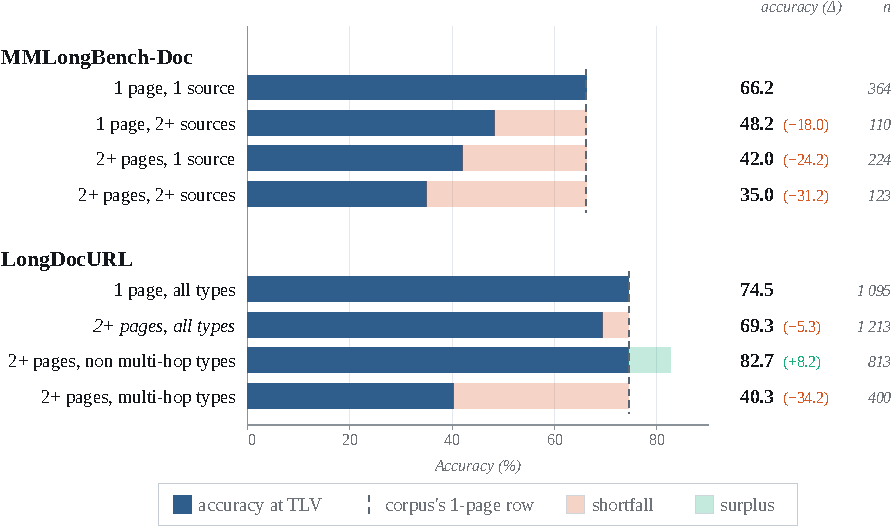
\includegraphics[width=0.8\columnwidth]{empirical/findings_figures/integration_multihop.pdf}
%   \caption[Accuracy by multi-hop evidence structure]{Accuracy by multi-hop evidence structure at the \textbf{TLV} rung. MMLongBench-Doc accuracy declines as evidence must be combined across additional sources and pages, while LongDocURL shows a large deficit only for question types established as genuinely multi-hop.}
%   \label{fig:integration_multihop}
% \end{figure}

% % GENERATED by tables/scripts/ -- do not edit by hand, re-run the script.
% Numbers read from results/tables/mmlongbench/*.csv and results/tables/longdocurl/*.csv.
% mmlongbench/mmlb_integration_prompt, longdocurl/ldu_integration_prompt
% Teal = accuracy on Ladder.tex's fixed [14,74] scale, bold = the better prompt in the row.
% Delta and the transitions: teal where CoT repairs (W->R), warm where it breaks (R->W). The deficit row
% washes warm with the size of the gap over [-30,0].
\definecolor{accteal}{HTML}{1BAF7A}
\definecolor{recwarm}{HTML}{D95926}
\definecolor{ngray}{HTML}{7A8494}
\begin{table}[ht]
\centering
\small
\setlength{\tabcolsep}{5pt}
\renewcommand{\arraystretch}{1.12}
\adjustbox{max width=\textwidth}{%
\begin{tabular}{@{}l r rr r @{\hskip 10pt} rr@{}}
\toprule
\textbf{Evidence structure} & \textcolor{ngray}{\scriptsize$n$} & \textbf{None} & \textbf{CoT} & \textbf{$\Delta$} & \textbf{R$\rightarrow$W} & \textbf{W$\rightarrow$R} \\
\midrule
\multicolumn{7}{l}{\emph{MMLongBench-Doc}} \\
1 page, 1 source & \textcolor{ngray}{\scriptsize364} & \cellcolor{accteal!52}\textbf{66.2} & \cellcolor{accteal!50}63.5 & \cellcolor{recwarm!10}-2.7 & \cellcolor{recwarm!21}9.3 & \cellcolor{accteal!15}6.6 \\
1 page, 2+ sources & \textcolor{ngray}{\scriptsize110} & \cellcolor{accteal!34}\textbf{48.2} & \cellcolor{accteal!32}46.4 & \cellcolor{recwarm!7}-1.8 & \cellcolor{recwarm!16}7.3 & \cellcolor{accteal!12}5.5 \\
2+ pages, 1 source & \textcolor{ngray}{\scriptsize224} & \cellcolor{accteal!28}42.0 & \cellcolor{accteal!33}\textbf{47.3} & \cellcolor{accteal!20}+5.4 & \cellcolor{recwarm!14}6.2 & \cellcolor{accteal!26}11.6 \\
2+ pages, 2+ sources & \textcolor{ngray}{\scriptsize123} & \cellcolor{accteal!21}35.0 & \cellcolor{accteal!27}\textbf{40.7} & \cellcolor{accteal!21}+5.7 & \cellcolor{recwarm!16}7.3 & \cellcolor{accteal!29}13.0 \\
\cmidrule(l){1-7}
\emph{Multi-hop pooled} & \textcolor{ngray}{\scriptsize457} & \cellcolor{accteal!28}41.6 & \cellcolor{accteal!31}\textbf{45.3} & \cellcolor{accteal!14}+3.7 & \cellcolor{recwarm!15}6.8 & \cellcolor{accteal!24}10.5 \\
% \emph{Integration deficit} &  & \cellcolor{recwarm!49}-24.6 & \cellcolor{recwarm!36}-18.2 & \cellcolor{accteal!24}+6.5 &  &  \\
\addlinespace
\multicolumn{7}{l}{\emph{LongDocURL}} \\
1 page & \textcolor{ngray}{\scriptsize1076} & \cellcolor{accteal!60}74.5 & -- & -- & -- & -- \\
2+ pages, other types & \textcolor{ngray}{\scriptsize746} & \cellcolor{accteal!60}82.7 & -- & -- & -- & -- \\
2+ pages, multi-hop types only & \textcolor{ngray}{\scriptsize347} & \cellcolor{accteal!26}40.3 & -- & -- & -- & -- \\
\bottomrule
\end{tabular}%
}
\caption[Chain-of-thought by evidence structure]{Effect of chain-of-thought across evidence structures at \textbf{TLV} with oracle pages.}
\label{tab:integration_prompt}
\end{table}
% {\footnotesize\raggedright
% Judge-scored accuracy (\%), accuracy rubric, answerable pools. MMLongBench-Doc's two prompts
% come from one run over the same questions. LongDocURL's uninstructed arm is its oracle ladder
% and its CoT arm is a separate run with the same model and budget; a CoT cell prints -- until
% that run is judged, and its None column is then over every question in the row. The
% multi-hop types are those whose multi-page questions mostly cannot be answered from one page
% (Table~\ref{tab:integration_multihop}); the other types are the rest of the multi-page
% pool.\par}
\begin{figure*}[h]
    \centering
    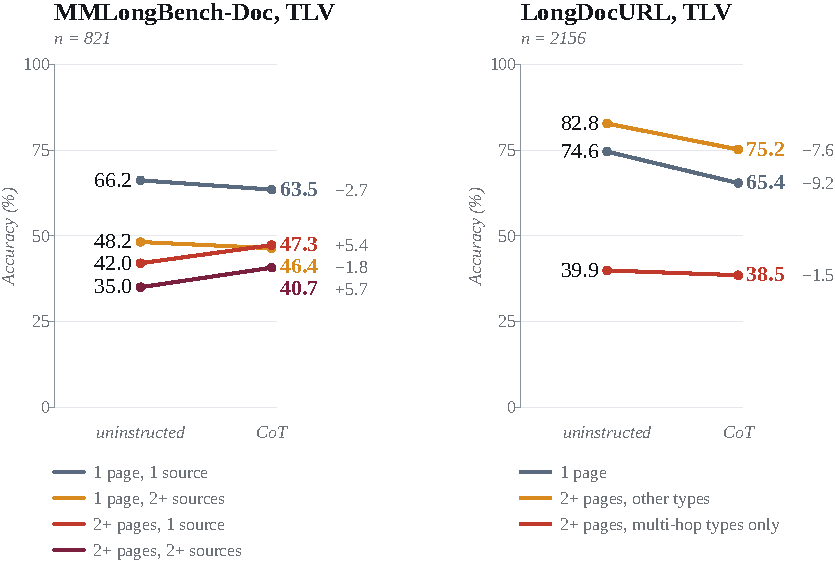
\includegraphics[width=0.7\linewidth]{empirical/findings_figures/integration_prompt.pdf}
    \caption[Effect of chain-of-thought across evidence structures]{Effect of chain-of-thought prompting across evidence structures at the \textbf{TLV} rung with oracle evidence pages. CoT selectively improves cross-page performance on MMLongBench-Doc, but does not produce the same gains on LongDocURL.}
    \label{fig:integration_prompt}
\end{figure*}

\paragraph{Chain-of-Thought Selectively Improves Cross-Page Integration.} Chain-of-thought does not improve reasoning uniformly across evidence structures or datasets (Figure~\ref{fig:integration_prompt}). On MMLongBench-Doc, it slightly reduces accuracy on single-page questions, from 66.2\% to 63.5\% for one-source questions and from 48.2\% to 46.4\% when several evidence sources occur on the same page. The effect reverses once evidence is distributed across pages: accuracy rises from 42.0\% to 47.3\% for one-source questions and from 35.0\% to 40.7\% when both pages and sources must be combined. The pooled integration deficit therefore narrows from 24.6 to 18.2 points. LongDocURL shows that this benefit is not universal. CoT reduces accuracy for single-page questions from 74.6\% to 65.4\% and for other multi-page questions from 82.8\% to 75.2\%, while its effect on multi-hop questions is much smaller, from 39.9\% to 38.5\%. This refines the usual motivation for chain-of-thought as a general aid to complex reasoning \citep{wei2022chain}. MP-VRDU methods similarly use explicit intermediate reasoning to combine evidence across document context \citep{jia2025leopard,xiong2026docr1}, but our results show that its value depends on the reasoning demands of the benchmark rather than on document length alone. On MMLongBench-Doc, part of the cross-page deficit identified in the original benchmark \citep{ma2024mmlongbench} is recoverable through a reasoning-only intervention; on LongDocURL, the same intervention provides no corresponding gain.

% GENERATED by tables/scripts/ -- do not edit by hand, re-run the script.
% Numbers read from results/tables/mmlongbench/*.csv.
% mmlb_integration_prompt_source
% Teal = accuracy on Ladder.tex's fixed [14,74] scale, bold = the better prompt in the row.
% Delta and the transitions: teal where CoT repairs (W->R), warm where it breaks (R->W).
% Source rows OVERLAP: a question citing Chart and Table counts under both, so All pools
% each question once rather than summing the rows.
\definecolor{accteal}{HTML}{1BAF7A}
\definecolor{recwarm}{HTML}{D95926}
\definecolor{ngray}{HTML}{7A8494}
\begin{table}[ht]
\centering
\small
\setlength{\tabcolsep}{5pt}
\renewcommand{\arraystretch}{1.12}
\begin{tabular}{@{}l r rr r @{\hskip 10pt} rr@{}}
\toprule
\textbf{Evidence source} & \textcolor{ngray}{\scriptsize$n$} & \textbf{None} & \textbf{CoT} & \textbf{$\Delta$} & \textbf{R$\rightarrow$W} & \textbf{W$\rightarrow$R} \\
\midrule
Text & \textcolor{ngray}{\scriptsize208} & \cellcolor{accteal!30}44.2 & \cellcolor{accteal!33}\textbf{46.6} & \cellcolor{accteal!9}+2.4 & \cellcolor{recwarm!15}6.7 & \cellcolor{accteal!20}9.1 \\
Layout & \textcolor{ngray}{\scriptsize98} & \cellcolor{accteal!29}42.9 & \cellcolor{accteal!31}\textbf{44.9} & \cellcolor{accteal!8}+2.0 & \cellcolor{recwarm!18}8.2 & \cellcolor{accteal!23}10.2 \\
Table & \textcolor{ngray}{\scriptsize137} & \cellcolor{accteal!22}36.5 & \cellcolor{accteal!33}\textbf{47.4} & \cellcolor{accteal!41}+10.9 & \cellcolor{recwarm!13}5.8 & \cellcolor{accteal!38}16.8 \\
Chart & \textcolor{ngray}{\scriptsize103} & \cellcolor{accteal!22}35.9 & \cellcolor{accteal!25}\textbf{38.8} & \cellcolor{accteal!11}+2.9 & \cellcolor{recwarm!13}5.8 & \cellcolor{accteal!20}8.7 \\
Figure & \textcolor{ngray}{\scriptsize173} & \cellcolor{accteal!29}\textbf{43.4} & \cellcolor{accteal!28}42.2 & \cellcolor{recwarm!4}-1.2 & \cellcolor{recwarm!17}7.5 & \cellcolor{accteal!14}6.4 \\
\midrule
\emph{All} & \textcolor{ngray}{\scriptsize457} & \cellcolor{accteal!28}41.6 & \cellcolor{accteal!31}\textbf{45.3} & \cellcolor{accteal!14}+3.7 & \cellcolor{recwarm!15}6.8 & \cellcolor{accteal!24}10.5 \\
\bottomrule
\end{tabular}
\caption[Chain-of-thought by evidence source]{Effect of chain-of-thought across evidence sources for multi-hop MMLongBench-Doc questions at \textbf{TLV} with oracle pages.}
\label{tab:integration_sources_cot}
\end{table}
% {\footnotesize\raggedright
% Judge-scored accuracy (\%), accuracy rubric, oracle pages. The pool is the multi-hop pooled
% row of Table~\ref{tab:integration_prompt}: every question except those citing one gold page
% and one evidence source. A question counts under every source it cites, so the rows overlap
% and All pools each question once.\par}

\paragraph{The Benefit Depends on the Evidence Being Integrated.} The improvement from chain-of-thought also varies substantially with evidence type (Table~\ref{tab:integration_sources_cot}). Among multi-hop questions, the largest gain occurs for tables, where accuracy increases from 36.5\% to 47.4\%, a 10.9-point improvement. Gains are much smaller for charts (+2.9 points), pure text (+2.4), and generalised text (+2.0), while figure questions decline slightly by 1.2 points. Chain-of-thought therefore appears most useful when cross-page integration requires explicit operations over structured evidence rather than simply more computation over any difficult input. This is consistent with the broader MP-VRDU literature, where multi-step reasoning is commonly introduced to decompose document-level questions and combine intermediate evidence \citep{suri2025visdom,jia2025leopard,xiong2026docr1}. At the same time, the weak or negative effect on several source types shows that additional reasoning is not intrinsically beneficial. Together with the structural breakdown above, the results suggest that chain-of-thought primarily mitigates a specific integration burden: relating complementary, and especially structured, evidence distributed across pages.

\subsubsection{Response Calibration}

\begin{figure}[h]
  \centering
  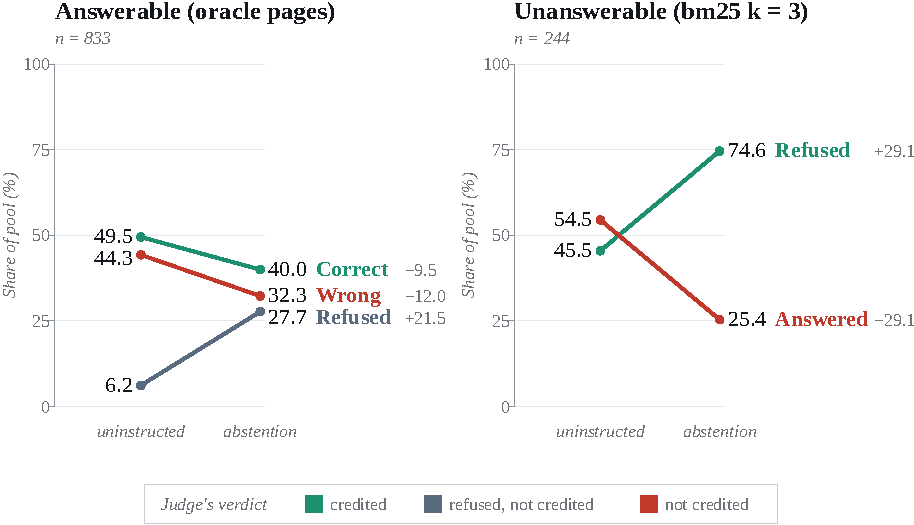
\includegraphics[width=0.7\columnwidth]{empirical/findings_figures/abstention_outcomes.pdf}
  \caption[Effect of abstention prompting]{Effect of targeted abstention prompting at the \textbf{TLV} rung. The instruction reduces unsupported answering when evidence is insufficient, but also increases refusal on answerable questions.}
  \label{fig:abstention_outcomes}
\end{figure}

\paragraph{The Reasoner Does Not Reliably Calibrate Evidence Sufficiency.} Targeted abstention prompting makes the reasoner substantially more conservative, but does not improve this decision selectively (Figure~\ref{fig:abstention_outcomes}). On unanswerable questions, refusal rises from 45.5\% to 74.6\%, substantially reducing unsupported answers. The same intervention raises refusal on answerable questions from 6.2\% to 27.7\%, while correct answers fall from 49.5\% to 40.0\%. Prior work similarly shows that prompting can shift context faithfulness and abstention behaviour \citep{zhou2023context}, while MMLongBench-Doc reports large differences between aggressive and conservative answering across models \citep{ma2024mmlongbench}. Our intervention shows that this operating point can also be shifted substantially within the same model. The reduction in unsupported answers therefore comes partly from a general increase in reluctance to answer, rather than a better distinction between sufficient and insufficient evidence.

% GENERATED by tables/scripts/ -- do not edit by hand, re-run the script.
% Numbers read from results/tables/analysis/*.csv.
% analysis/faithfulness_answerable_accuracy_source (results.errcat.jsonl)
% Shade ranges are fitted to the values present:
% Acc.: accteal over [26.4, 51.0]  % Abst.: neutral over [0.8, 35.5]  % Inc.: recwarm over [30.3, 50.0]
\definecolor{accteal}{HTML}{1BAF7A}
\definecolor{neutral}{HTML}{5B6B7F}
\definecolor{recwarm}{HTML}{D95926}
\definecolor{ngray}{HTML}{7A8494}
\begin{table}[ht]
\centering
\small
\setlength{\tabcolsep}{5pt}
\renewcommand{\arraystretch}{1.12}
\begin{tabular}{@{}l r rrr @{\hskip 10pt} rrr@{}}
\toprule
 & & \multicolumn{3}{c}{\textbf{No instruction}} & \multicolumn{3}{c}{\textbf{Abstention instruction}} \\
\cmidrule(lr){3-5}\cmidrule(l){6-8}
\textbf{Evidence source} & \textcolor{ngray}{\scriptsize$n$} & \textbf{Acc.} & \textbf{Abst.} & \textbf{Inc.} & \textbf{Acc.} & \textbf{Abst.} & \textbf{Inc.} \\
\midrule
Text & \textcolor{ngray}{\scriptsize286} & \cellcolor{accteal!60}\textbf{51.0} & \cellcolor{neutral!11}7.3 & \cellcolor{recwarm!34}41.6 & \cellcolor{accteal!42}\textbf{43.7} & \cellcolor{neutral!40}24.1 & \cellcolor{recwarm!6}32.2 \\
Layout & \textcolor{ngray}{\scriptsize118} & \cellcolor{accteal!56}49.2 & \cellcolor{neutral!0}\textbf{0.8} & \cellcolor{recwarm!60}\textbf{50.0} & \cellcolor{accteal!37}41.5 & \cellcolor{neutral!32}\textbf{19.5} & \cellcolor{recwarm!26}39.0 \\
Table & \textcolor{ngray}{\scriptsize208} & \cellcolor{accteal!45}44.7 & \cellcolor{neutral!10}6.7 & \cellcolor{recwarm!56}48.6 & \cellcolor{accteal!30}38.5 & \cellcolor{neutral!51}30.3 & \cellcolor{recwarm!3}31.2 \\
Chart & \textcolor{ngray}{\scriptsize178} & \cellcolor{accteal!40}42.7 & \cellcolor{neutral!11}7.3 & \cellcolor{recwarm!60}\textbf{50.0} & \cellcolor{accteal!0}26.4 & \cellcolor{neutral!42}25.3 & \cellcolor{recwarm!55}\textbf{48.3} \\
Figure & \textcolor{ngray}{\scriptsize290} & \cellcolor{accteal!39}42.4 & \cellcolor{neutral!12}7.6 & \cellcolor{recwarm!60}\textbf{50.0} & \cellcolor{accteal!19}34.1 & \cellcolor{neutral!60}35.5 & \cellcolor{recwarm!0}30.3 \\
\midrule
\emph{All} & \textcolor{ngray}{\scriptsize833} & \cellcolor{accteal!56}49.5 & \cellcolor{neutral!9}6.2 & \cellcolor{recwarm!43}44.3 & \cellcolor{accteal!33}40.0 & \cellcolor{neutral!47}27.7 & \cellcolor{recwarm!6}32.3 \\
\bottomrule
\end{tabular}
\caption{Refusal outcomes by evidence source under targeted abstention prompting at \textbf{TLV}. False abstention is more frequent for visually and structurally demanding evidence, suggesting that reasoning difficulty influences the decision to refuse.}
\label{tab:abstention_sources}
\end{table}


\paragraph{Reasoning Difficulty Is Mistaken for Evidence Insufficiency.} False abstention also rises with the difficulty of interpreting the supplied evidence. Under the abstention instruction, refusal reaches 35.5\% for figure questions and 30.3\% for table questions, compared with 25.3\% for charts and 24.1\% for text (Table~\ref{tab:abstention_sources}). Since these questions receive their oracle pages and the full \textbf{TLV} representation, the higher refusal rates cannot be attributed to evidence absence. Difficult evidence instead appears more likely to be treated as insufficient evidence. Response calibration therefore depends not only on whether support is present, but also on the reasoner's confidence in interpreting it, which helps explain why stronger abstention instructions trade unsupported answers for false refusals rather than cleanly separating the two.

\begin{figure}[!p]
  \centering
  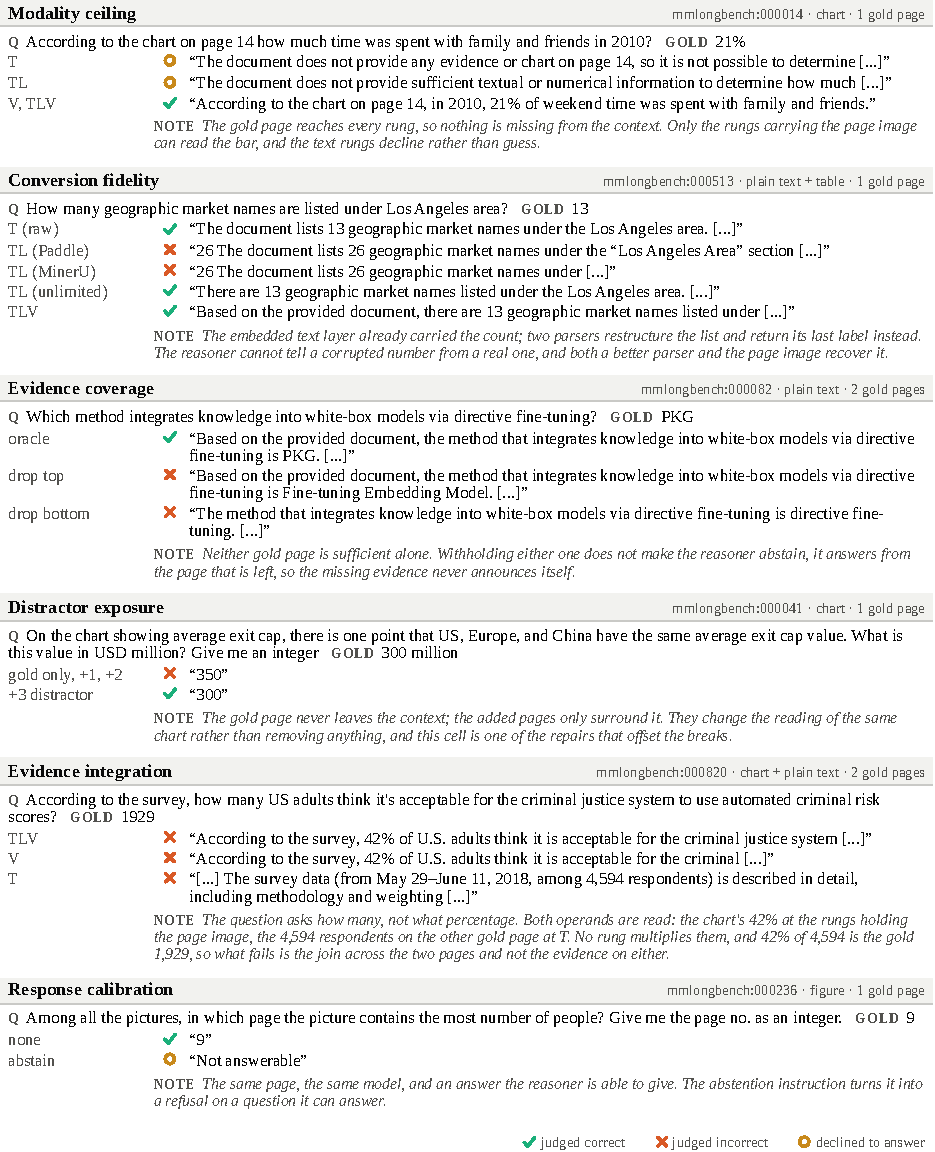
\includegraphics[width=\columnwidth]{empirical/findings_figures/worked_examples.pdf}
  \caption[Worked examples of the six failure mechanisms]{Worked examples of the six failure mechanisms, one question each, from MMLongBench-Doc under Qwen3-VL-8B. Every band gives the question, its gold answer, and what the reasoner returned under each condition that mechanism is tested by, marked with the judge's verdict; the quotations are the model's own output, elided at [\ldots].}
  \label{fig:worked_examples}
\end{figure}

\section{Error Analysis}
\label{sec:emp_error_analysis}

The error taxonomy provides a finer view of how the reasoner fails once representation and evidence selection are controlled. Unlike the preceding analyses, each category is reported as a share of the full question pool for that condition, allowing direct comparison across prompt modes and evidence sources.

\subsection{Prompt Mode}

% \input{empirical/analysis/error_profile}
\begin{figure}[h]
  \centering
  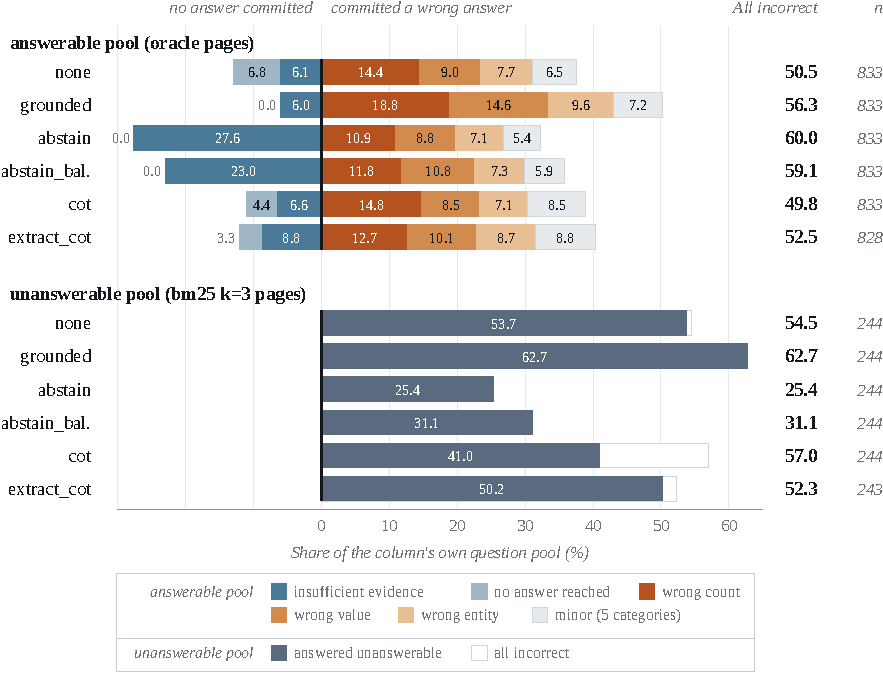
\includegraphics[width=0.8\columnwidth]{empirical/analysis/error_profile.pdf}
  \caption[Error profile by prompt mode]{Error profile by prompt mode on answerable and unanswerable questions.}% Answerable errors are decomposed by failure type, while the unanswerable pool reports unsupported answers. Grounding primarily shifts non-commitment into explicit errors, while chain-of-thought leaves answerable accuracy largely unchanged and increases unsupported answering on unanswerable questions.}
  \label{fig:error_profile}
\end{figure}

The error distribution changes substantially with the reasoning instruction, showing that prompting alters the form of failure rather than uniformly removing it. Grounding largely eliminates cases where the model fails to reach an answer, but this is offset by committed errors such as incorrect counts, values, and entities. The abstention instruction shifts the distribution more strongly toward \texttt{insufficient\_evidence}, consistent with the calibration results above: it prevents some unsupported answers but also introduces refusals on answerable questions. The \texttt{abstain\_balanced} variant produces a very similar profile despite explicitly encouraging the model to answer when evidence is sufficient, suggesting that this trade-off is not easily removed through wording alone. Chain-of-thought produces a different redistribution, changing the mix of substantive answer errors without the same increase in abstention, while \texttt{extract\_cot} remains close to ordinary \texttt{cot} despite adding an explicit evidence-extraction step. Prompting therefore changes how the reasoner fails, but no mode removes the underlying reasoning errors across the board.


\subsection{Evidence Source}
\label{sec:error_evidence_integration}

\begin{figure}[ht]
  \centering
  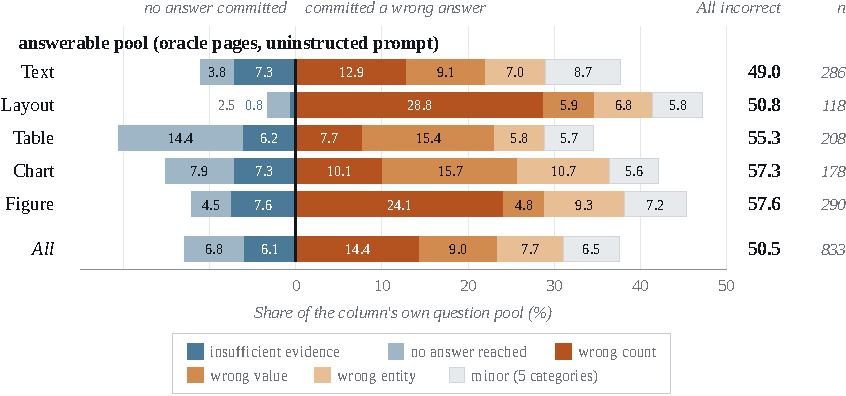
\includegraphics[width=0.8\columnwidth]{empirical/analysis/error_sources.pdf}
  \caption[Error profile by evidence source]{Error profile by evidence source on the answerable pool with oracle pages and no prompt instruction.}% Different evidence types produce distinct failure patterns: layout and figure questions are dominated by wrong-count errors, while tables and charts more often produce wrong-value errors.}
  \label{fig:error_sources}
\end{figure}

Error type also varies substantially with the evidence a question requires. Under the uninstructed oracle-page condition, 50.5\% of answerable questions are incorrect overall, but the dominant failure differs by source. Layout and figure questions are particularly prone to \texttt{wrong\_count} errors, which account for 28.8\% and 24.1\% of their respective pools, compared with 14.4\% overall. Tables and charts instead show the highest \texttt{wrong\_value} rates, at 15.4\% and 15.7\%, suggesting that structured quantitative evidence more often fails during value extraction, comparison, or combination. Tables also stand out for \texttt{no\_answer\_reached}, which occurs on 14.4\% of questions, more than twice the pooled rate of 6.8\%. These differences indicate that providing the required multimodal evidence does not make downstream reasoning uniform: spatial and visual content more often fails during identification or aggregation, while quantitative structures produce a different mixture of extraction and comparison errors. The remaining failures are distributed across entity, list, abstention, and other categories, reinforcing that MP-VRDU difficulty depends not only on whether the evidence is available, but also on the operations required to interpret its particular form.

% \begin{figure}[ht]
%   \centering
%   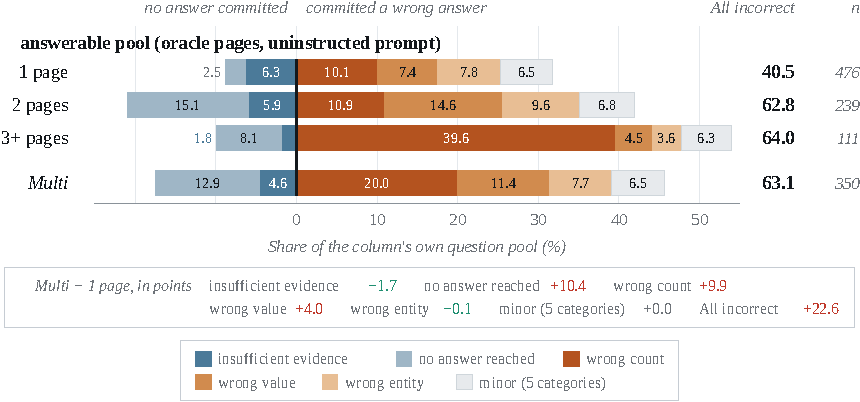
\includegraphics[width=0.8\columnwidth]{empirical/analysis/error_integration.pdf}
%   \caption[Error profile by evidence-page count]{Error profile by evidence-page count on the answerable pool with oracle pages and no prompt instruction. Moving from single-page to multi-page questions sharply increases non-commitment, wrong-count, and wrong-value errors, while insufficient-evidence errors do not increase.}
%   \label{fig:error_integration}
% \end{figure}

% \paragraph{Cross-Page Integration Amplifies Reasoning Errors.} Moving from one page to multiple pages produces a clear shift in the error profile. Relative to single-page questions, the pooled multi-page set shows a 10.4-point increase in no-answer-reached errors, a 9.9-point increase in wrong-count errors, and a 4.0-point increase in wrong-value errors. By contrast, insufficient-evidence errors decrease slightly. Since every oracle page is supplied, these failures are not caused by missing evidence, but by difficulty combining and operating over evidence that is already present. The largest change also occurs when moving from one page to two pages, with total incorrect rising from 40.5\% to 62.8\%, while 3+ pages reach 64.0\%. This suggests that crossing the page boundary itself introduces much of the reasoning burden, rather than error increasing proportionally with each additional page.

\section{Practical Discussion}
\label{sec:practical_discussion}

The preceding experiments isolate where MP-VRDU systems fail. We now consider what those findings imply for system design and deployment. Rather than treating representation, retrieval, and reasoning independently, the results suggest that compute should be allocated across the pipeline according to where information is most likely to be lost and where additional capacity can still recover it.
f
\subsection{Encoding Cost and Fidelity}
\label{sec:discussion_representation}

% GENERATED by tables/scripts/ -- do not edit by hand, re-run the script.
% Numbers read from results/tables/analysis/*.csv (cost) and mmlongbench/*.csv (OOM).
% deployment_rungs (results.errcat.jsonl), oom_frontier
% Teal deepens with accuracy on Ladder.tex's fixed [14,74] scale, so a cell here reads
% against a cell there. Warm wash on input tokens and on the OOM rate: both are costs.
\definecolor{accteal}{HTML}{1BAF7A}
\definecolor{recwarm}{HTML}{D95926}

\begin{table}[ht]
\centering
\small
\setlength{\tabcolsep}{5pt}
\renewcommand{\arraystretch}{1.12}
\begin{tabular}{@{}l r rrr r rr r@{}}
\toprule
 & & \multicolumn{3}{c}{\textbf{Input tokens}} & & \multicolumn{2}{c}{\textbf{Output}} & \\
\cmidrule(lr){3-5}\cmidrule(lr){7-8}
\textbf{Rung} & \textbf{Acc.} & \textbf{text} & \textbf{visual} & \textbf{total} & \textbf{prefill s} & \textbf{tok} & \textbf{decode s} & \textbf{OOM \%} \\
\midrule
\textbf{T} & \cellcolor{accteal!15}29.0 & 932 & 0 & \cellcolor{recwarm!19}932 & 1.4 & 115 & 5.7 & \cellcolor{recwarm!2}1.2 \\
\textbf{TL} & \cellcolor{accteal!22}35.7 & 1632 & 0 & \cellcolor{recwarm!33}1632 & 1.8 & 133 & 6.6 & \cellcolor{recwarm!9}6.7 \\
\textbf{TV} & \cellcolor{accteal!36}50.1 & 929 & 851 & \cellcolor{recwarm!36}1780 & -- & 140 & -- & -- \\
\textbf{TLV} & \cellcolor{accteal!36}49.5 & 1632 & 857 & \cellcolor{recwarm!51}2488 & 26.3 & 136 & 6.7 & \cellcolor{recwarm!15}11.2 \\
\textbf{V} & \cellcolor{accteal!29}42.6 & 38 & 857 & \cellcolor{recwarm!18}894 & 29.0 & 139 & 7.1 & \cellcolor{recwarm!1}0.8 \\
\bottomrule
\end{tabular}
\caption{Cost of each representation rung. Accuracy and token counts are means over the answerable pool under the error-taxonomy judge; the two latency columns and the OOM rate are measured separately on 2$\times$16\,GB V100s.}
\label{tab:deployment_rungs}
\end{table}

% {\footnotesize\raggedright
% Uninstructed prompt, oracle pages, answerable pool, judged under the error-taxonomy
% rubric. Accuracy is the same judge and the same pool as Table~\ref{tab:ladder_source} and
% shares its teal scale, so a cell here reads against a cell there; it is NOT interchangeable
% with a level from a table scored by the main report's judge.
% \textbf{Input and output cost are set by different things and must be read apart.} Input
% tokens and prefill time are fixed by the representation: TL adds parser markdown to T, V
% replaces text with about 860 visual tokens, and TLV pays for both. Output tokens and decode
% time are set by the prompt and the decode budget, so they barely move across rungs; a rung
% that appears to decode more is one whose longer input drew a longer answer. The two halves do
% not sum to end-to-end latency, which also carries scheduling and detokenisation.
% \textbf{The three right-hand columns are measured on different rows from the accuracy.}
% Latency and the OOM rate both read the preserved pre-recovery V100 snapshots, because this
% pool's failed cells were re-run on an H100: the live rows carry that machine's timings, where
% the same cells prefill in 0.06--0.18\,s and \textbf{TL}$\rightarrow$\textbf{TLV} rises
% 1.8-fold rather than 13.6-fold, which prices the table on hardware the study does not deploy
% on. Latency is therefore a mean over the matched cells every ladder config ran ($n=831/761/717/834$
% by rung), which excludes the cells that OOMed and so prices a lighter input than the token
% columns show: \textbf{TLV} averages 1,540 tokens over those cells against 2,488 over the
% full pool. The OOM rate is the same snapshot pooled over its page-count buckets at medium
% resolution. \textbf{TV} never ran on a V100, so it carries no latency and no rate; its cost
% sits in the token columns, which are machine-independent. Latency is wall clock and a scale
% rather than an absolute. Table~\ref{tab:reasoner_cost_all} gives the same two columns for
% every reasoner configuration, grouped by measuring machine.
% \textbf{TV is the rung that pays for itself, and under this judge it beats TLV outright.}
% It scores 50.1 against 49.5 on 708 fewer input tokens, so \textbf{TLV} is dominated: it costs
% more and returns less. The parser's markdown does not merely earn little once the page image
% is present, it is a net loss. Read the two accuracies as close rather than as a ranking: TV is
% measured over all 847 cells and the other rungs over the 833 the sweep judged, and the
% difference is well inside either interval.\par}

Table~\ref{tab:deployment_rungs} shows that representation cost depends on both the channels retained and how they are processed. At the medium resolution, \textbf{V} averages 857 visual tokens and 894 total input tokens per question, comparable to the 932 tokens of \textbf{T}; the largest context instead comes from combining channels, with \textbf{TLV} averaging 2,488 tokens from 1,632 text and 857 visual tokens. Visual processing nevertheless carries a substantial compute cost, with \textbf{V} and \textbf{TLV} requiring 29.0 and 26.3\,s of measured prefill time compared with 1.4--1.8\,s for the text-only rungs, while output length and decoding time remain comparatively stable. The richest representation also produces the highest measured OOM rate at 11.2\%, compared with 0.8\% for \textbf{V}. Importantly, additional representation cost does not always translate into higher accuracy: \textbf{TV} reaches 50.1\% against 49.5\% for \textbf{TLV} while averaging 1,780 rather than 2,488 input tokens, suggesting that embedded text paired with vision is a strong option for born-digital documents where parsing adds little once the page image is available. This does not extend to scanned documents, which lack a reliable embedded-text channel and therefore still benefit from parser-derived text. Likewise, the resolution sweep shows that additional visual fidelity is most useful for dense tables, charts, and other visually dependent evidence rather than uniformly across questions. Representation should therefore be selected around the target workload: retain text and vision where both carry complementary evidence, avoid parser overhead where embedded text is already sufficient, and spend additional visual resolution only where legibility is likely to constrain performance.

\subsection{Retrieval Quality and Efficiency}
\label{sec:discussion_retrieval}

\begin{figure}[ht]
  \centering
  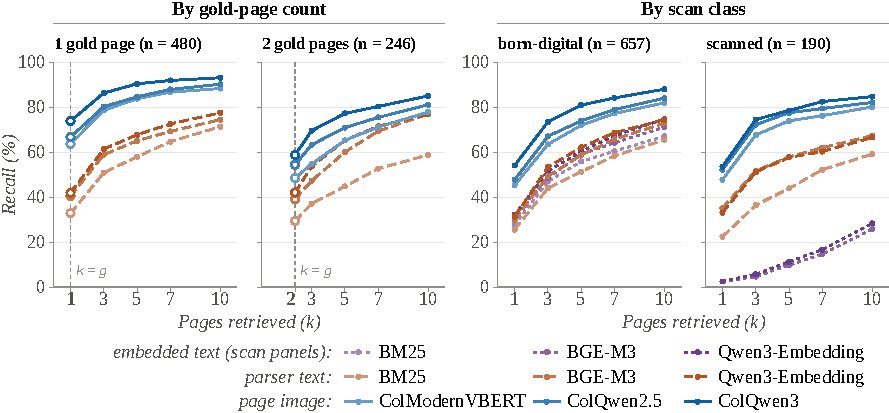
\includegraphics[width=0.95\columnwidth]{empirical/discussion/retrieval.pdf}
  \caption[Retrieval recall across depth and document type]{Retrieval recall on MMLongBench-Doc across retrieval depth, gold-page count, and document type. Recall increases with depth, questions requiring several evidence pages remain harder to cover, and visual retrieval is more robust across born-digital and scanned documents.}
  \label{fig:retrieval}
\end{figure}

The selection findings suggest that retrieval should be configured primarily around evidence coverage, with the retriever and depth chosen according to the document distribution and the amount of downstream context the system can afford to process. Figure~\ref{fig:retrieval} shows that recall rises consistently with depth: ColQwen3 increases from 54.1\% at \(k=1\) to 87.4\% at \(k=10\), while the strongest joint text--vision configuration rises from 58.7\% to 89.7\%. This gain comes at the expected loss of precision, but the selection experiments show why that trade can be worthwhile: omitting required evidence is substantially more damaging than introducing a moderate number of additional pages, and some non-gold pages can even supply useful contextual information. Multi-page questions further strengthen this argument because complete coverage is harder when several required pages must all be recovered. Retrieval representation introduces a second deployment choice. Embedded-text retrieval avoids document parsing and is effective on born-digital documents, but its reliability falls on scans where the text layer is absent or sparse. Parser-based text retrieval adds preprocessing cost while recovering much of this robustness, whereas visual retrievers remain comparatively consistent across both document types. A practical system should therefore favour recall where downstream evidence filtering is available, while choosing between text, parsed-text, visual, or joint retrieval according to the document mix and preprocessing budget rather than treating one retrieval representation as universally preferable.

\subsection{Reasoner Capability and Deployment Trade-offs}
\label{sec:discussion_reasoner}

% GENERATED by tables/scripts/ -- do not edit by hand, re-run the script.
% Numbers read from results/tables/mmlongbench/*.csv.
% reasoner_unified, weight_footprint
% Teal deepens with accuracy on Ladder.tex's fixed [14,74] scale, so a cell here reads
% against a cell there. GB carries its own warm scale over [4,25]: a footprint is a
% cost, not an accuracy. Empty rows are models declared but not yet run.
\definecolor{accteal}{HTML}{1BAF7A}
\definecolor{recwarm}{HTML}{D95926}

\begin{table}[ht]
\centering
\small
\setlength{\tabcolsep}{4pt}
\begin{tabular}{lrrrrr}
\toprule
\textbf{Model / config} & \textbf{T} & \textbf{TL} & \textbf{TLV} & \textbf{V} & \textbf{GB} \\
\midrule
\multicolumn{6}{l}{\emph{Scale (Qwen3-VL, bf16)}} \\
\quad 2B & \cellcolor{accteal!11}24.7 & \cellcolor{accteal!18}31.9 & \cellcolor{accteal!24}38.3 & \cellcolor{accteal!18}31.9 & \cellcolor{recwarm!1}4.3 \\
\quad 4B & \cellcolor{accteal!18}32.3 & \cellcolor{accteal!25}38.6 & \cellcolor{accteal!36}50.4 & \cellcolor{accteal!28}42.4 & \cellcolor{recwarm!13}8.9 \\
\quad 8B & \cellcolor{accteal!18}31.9 & \cellcolor{accteal!24}38.4 & \cellcolor{accteal!38}52.4 & \cellcolor{accteal!32}45.5 & \cellcolor{recwarm!35}17.5 \\
\quad 32B & \cellcolor{accteal!22}35.5 & \cellcolor{accteal!30}43.9 & \cellcolor{accteal!46}59.6 & \cellcolor{accteal!43}56.7 & \cellcolor{recwarm!55}66.7 \\
\cmidrule(lr){1-6}
\multicolumn{6}{l}{\emph{Precision (Qwen3-VL-8B)}} \\
\quad 16-bit & \cellcolor{accteal!18}31.9 & \cellcolor{accteal!24}38.4 & \cellcolor{accteal!38}52.4 & \cellcolor{accteal!32}45.5 & \cellcolor{recwarm!35}17.5 \\
\quad 8-bit & \cellcolor{accteal!18}32.5 & \cellcolor{accteal!24}37.9 & \cellcolor{accteal!40}53.6 & \cellcolor{accteal!32}45.7 & \cellcolor{recwarm!16}10.3$^{\sim}$ \\
\quad 4-bit & \cellcolor{accteal!18}31.8 & \cellcolor{accteal!25}39.4 & \cellcolor{accteal!38}51.8 & \cellcolor{accteal!32}45.5 & \cellcolor{recwarm!7}6.8$^{\sim}$ \\
\cmidrule(lr){1-6}
\multicolumn{6}{l}{\emph{Matched budget ($\sim$17--20\,GB)}} \\
\quad 8B, 16-bit & \cellcolor{accteal!18}31.9 & \cellcolor{accteal!24}38.4 & \cellcolor{accteal!38}52.4 & \cellcolor{accteal!32}45.5 & \cellcolor{recwarm!35}17.5 \\
\quad 32B, 4-bit & \cellcolor{accteal!23}37.0 & \cellcolor{accteal!28}42.1 & \cellcolor{accteal!45}59.1 & \cellcolor{accteal!38}52.3 & \cellcolor{recwarm!42}20.0$^{\sim}$ \\
\cmidrule(lr){1-6}
\multicolumn{6}{l}{\emph{Family (8B class, bf16)}} \\
\quad Qwen3-VL-8B & \cellcolor{accteal!18}31.9 & \cellcolor{accteal!24}38.4 & \cellcolor{accteal!38}52.4 & \cellcolor{accteal!32}45.5 & \cellcolor{recwarm!35}17.5 \\
\quad InternVL3-8B & \cellcolor{accteal!5}19.3 & \cellcolor{accteal!11}25.3 & \cellcolor{accteal!19}32.6 & \cellcolor{accteal!10}24.1 & \cellcolor{recwarm!31}15.9 \\
\quad GLM-4.6V-Flash (9B dense) & \cellcolor{accteal!12}25.9 & \cellcolor{accteal!19}32.9 & \cellcolor{accteal!29}42.7 & \cellcolor{accteal!17}30.9 & \cellcolor{recwarm!43}20.6 \\
\quad MiniCPM-V-4.5 (8B) & \cellcolor{accteal!17}30.7 & \cellcolor{accteal!24}38.1 & \cellcolor{accteal!46}60.1 & \cellcolor{accteal!39}53.3 & \cellcolor{recwarm!35}17.4 \\
\quad Llama-3.2-11B-Vision & \cellcolor{accteal!12}26.5 & \cellcolor{accteal!20}34.3 & \cellcolor{accteal!19}33.3 & \cellcolor{accteal!11}25.3 & \cellcolor{recwarm!45}21.3 \\
\cmidrule(lr){1-6}
\multicolumn{6}{l}{\emph{Scale (Gemma-3, bf16)}} \\
\quad 4B & \cellcolor{accteal!8}22.1 & \cellcolor{accteal!16}30.5 & \cellcolor{accteal!26}39.5 & \cellcolor{accteal!20}33.6 & \cellcolor{recwarm!12}8.6 \\
\quad 12B & \cellcolor{accteal!16}30.5 & \cellcolor{accteal!23}36.9 & \cellcolor{accteal!34}48.1 & \cellcolor{accteal!28}41.6 & \cellcolor{recwarm!53}24.4 \\
\quad 27B & \cellcolor{accteal!19}32.8 & \cellcolor{accteal!26}40.0 & \cellcolor{accteal!38}52.0 & \cellcolor{accteal!31}44.6 & \cellcolor{recwarm!55}54.9 \\
% \cmidrule(lr){1-6}
% \multicolumn{6}{l}{\emph{Sparse (mixture of experts)}} \\
% \quad Qwen3-VL-30B-A3B-Instruct & -- & -- & -- & -- & -- \\
\cmidrule(lr){1-6}
\multicolumn{6}{l}{\emph{Reasoning variant (Qwen3-VL-8B)}} \\
\quad Instruct & \cellcolor{accteal!18}31.9 & \cellcolor{accteal!24}38.4 & \cellcolor{accteal!38}52.4 & \cellcolor{accteal!32}45.5 & \cellcolor{recwarm!35}17.5 \\
\quad Thinking & \cellcolor{accteal!21}34.8 & \cellcolor{accteal!29}42.9 & \cellcolor{accteal!48}62.2 & \cellcolor{accteal!38}52.1 & \cellcolor{recwarm!35}17.5 \\
\bottomrule
\end{tabular}
\caption{Reasoner accuracy across scale, precision, matched budget and family. Accuracy (\%) on oracle pages over the full answerable pool; GB is the model weight footprint, not peak VRAM.}
\label{tab:reasoner}
\end{table}

% {\footnotesize\raggedright
% Accuracy (\%) on oracle pages at medium resolution, uninstructed prompt, full answerable
% pool ($n=847$); per-cell $n$ is omitted for space and runs 640--847, thinnest at TLV where
% OOM attrition is largest. Teal shares Table~\ref{tab:ladder_source}'s scale, so a cell here
% reads against a cell there. \textbf{GB} is the model weight footprint, carrying its own warm
% scale because a footprint is a cost rather than an accuracy; $^{\sim}$ marks a footprint
% derived from the 16-bit weights rather than measured. Peak VRAM was device-0 only and is not
% reported. \textbf{Empty rows are models declared in the methodology that have not been run.}
% \textbf{Scale buys the most on the visual rungs} and quantization is nearly free: 4-bit
% costs the 8B 0.6 points at TLV for 61\% of the weights. At a matched memory budget the
% quantized 32B beats the 16-bit 8B at every rung, which is the practical reading of the
% table: given a fixed card, a larger model at lower precision is the better buy. \textbf{Family
% choice costs more than either}, and in both directions: at essentially the same footprint
% InternVL3-8B loses 19.8 points to Qwen3-VL-8B at TLV while MiniCPM-V-8B gains 9.5, a spread
% wider than four times the scale step from 2B to 32B. The family is the first decision, not
% the last. MiniCPM-V's thinner $n$ at TLV (640) is OOM attrition, so read that cell as a
% surviving-question rate rather than a like-for-like win. \\textbf{Llama-3.2-11B-Vision is the
% one family that loses accuracy when the pages are added}: it peaks at TL (34.3) and drops to
% 33.3 at TLV and 25.3 at V, so for it the ladder inverts and the parser text is the better
% input. Every other family gains on the visual rungs.
% \textbf{The Thinking checkpoint beats the Instruct model it forks from at every rung},
% by 2.9 to 9.8 points and most at TLV, the largest single move in the table; its value is in the
% hop split rather than the level, since it nearly closes the multi-page deficit
% ($-$9.1 against $-$19.9). \textbf{GLM-4.6V} is the 107B mixture-of-experts member of the
% GLM line, a different architecture from the 9B dense Flash variant above rather than a
% size option of it, and has not been run.\par}

Table~\ref{tab:reasoner} shows that reasoner deployment is not simply a choice of parameter count, but a trade-off between model family, scale, numerical precision, memory, and the type of reasoning required. Within Qwen3-VL, scaling from 2B to 32B raises TLV accuracy from 38.3\% to 59.6\%, but the reasoning experiments show that larger models do not remove the single-to-multi-page integration deficit, so scale improves capability without directly resolving every failure mode. Models of similar size also differ substantially: Qwen3-VL-8B reaches 52.4\% at TLV compared with 32.6\% for InternVL3-8B, showing that nominal parameter count alone is a poor deployment criterion. Quantisation provides the clearest way to preserve model capacity under a fixed memory budget. Qwen3-VL-8B changes only from 52.4\% at 16-bit to 51.8\% at 4-bit while reducing its weight footprint from 17.5\,GB to approximately 6.8\,GB, and the 32B model at 4-bit reaches 59.1\% at approximately 20\,GB, outperforming the full-precision 8B model at a similar memory budget. The 4B model also remains close to the 8B model on several conditions, suggesting that smaller checkpoints can still be attractive where throughput matters more than peak accuracy. Under tight VRAM constraints, preserving scale through quantisation can therefore be preferable to immediately selecting a smaller full-precision model, but the choice should still account for model family and latency because reduced weight precision does not guarantee faster decoding on all hardware.


\section{Conclusion}
\label{sec:emp-conc}

This chapter examined MP-VRDU failure through controlled attribution across representation, selection, and reasoning. The results show that vision is necessary but remains complementary to text, that missing required evidence is substantially more damaging than moderate distractor exposure, and that cross-page integration remains difficult even when all required evidence is supplied. The analysis further shows that prompt interventions can shift error behaviour without necessarily improving underlying reasoning or calibration. Together, these findings show that MP-VRDU failure is distributed across the evidence pipeline and that end-to-end accuracy alone is insufficient to identify the mechanism responsible.

% ============================================================================
%  Conclusion
% ============================================================================
\chapter{Method and Conclusion}
\label{ch:conclusion}

Chapter~\ref{ch:survey} uses an evidence-management perspective to organise the rapidly developing MP-VRDU literature, while Chapter~\ref{ch:empirical} examines where current systems fail through controlled attribution across representation, selection, and reasoning. Although these chapters address different questions, together they provide both a structured view of how MP-VRDU systems are built and empirical guidance on which design choices most strongly affect their behaviour. This chapter brings those contributions together by translating them into a deliberately simple working pipeline before considering the broader challenges and conclusions that follow.

\section{A Simple Adaptive-Trajectory Method}
\label{sec:simple_method}

We translate the evidence-management perspective of Chapter~\ref{ch:survey} and the empirical findings of Chapter~\ref{ch:empirical} into a deliberately simple MP-VRDU pipeline. The aim is not to introduce a new specialised backbone or complex orchestration framework, but to test whether the preceding findings provide a useful basis for system design when combined in a complete working method. Where appropriate, the pipeline uses mechanisms already established in the literature, including iterative evidence memory~\citep{jain2025simpledoc} and answer verification~\citep{zhu2026doclens}. We then evaluate whether this combination can remain competitive with substantially more specialised systems using similar open-weight models under a fixed hardware budget.

\subsection{Method Overview}
\label{sec:simple_adaptive_method}

\begin{figure}[t]
    \centering
    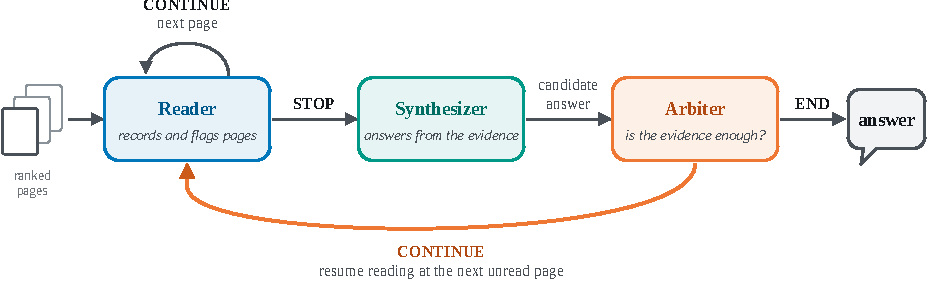
\includegraphics[width=0.78\textwidth]{method/simple_method.pdf}
    \caption{Architecture of the proposed method.}
    \label{fig:simple_method_arch}
\end{figure}

The pipeline separates evidence acquisition from final evidence presentation and reasoning. A retriever first ranks the document pages, after which three roles implemented by the same vision-language model operate in a fixed loop (Figure~\ref{fig:simple_method_arch}). The \texttt{reader} acquires and records evidence, the \texttt{synthesizer} produces a candidate answer from the accumulated evidence, and the \texttt{arbiter} either accepts that answer or requests further reading. This process continues until the answer is accepted or the reading budget is exhausted. Full implementation details, including the role-specific prompts and system configuration, are provided in Appendix~\ref{app:simple_method_details}.

\paragraph{\texttt{Reader}: Evidence Acquisition and Recall-Oriented Selection.}
The \texttt{reader} traverses pages in retrieval-ranked order using complementary textual and visual representations. Unlimited-OCR~\cite{yin2026unlimited} supplies parser text, while the page image preserves information that may be lost or difficult to recover through parsing alone. Each turn distils the current page into a compact evidence record that is appended to a persistent evidence memory. The \texttt{reader} additionally performs recall-oriented page selection, flagging pages that the answer may depend on, including uncertain but potentially relevant evidence. This separates broad evidence acquisition from high-fidelity evidence presentation: compact records retain context from useful inspected pages, while only flagged pages are later reintroduced in full multimodal form. Once the minimum reading depth has been reached, the \texttt{reader} may propose \texttt{STOP} when it judges the accumulated evidence sufficient for answer synthesis.

\paragraph{\texttt{Synthesizer}: Evidence Integration and Premise Validation.}
The \texttt{synthesizer} receives the accumulated evidence in document order when reading stops. Flagged pages are restored in full through parser text and page images, while other useful pages remain represented by their compact evidence records. This provides broad document context while reserving the final multimodal context for the evidence judged most likely to be answer-bearing. The \texttt{synthesizer} performs cross-page evidence integration to produce a candidate answer and explicitly validates the premises and presuppositions of the question against the supplied evidence. If the required support is absent, it must identify the unresolved evidence requirement before returning \emph{Not answerable}. This separates answer generation from evidential sufficiency assessment, reflecting the Chapter~\ref{ch:empirical} finding that evidence availability alone does not guarantee correct integration or calibration.

\paragraph{\texttt{Arbiter}: Evidential Verification and Adaptive Re-Acquisition.}
The \texttt{arbiter} receives the evidence memory, the candidate answer, and the same flagged pages in full textual and visual form. Access to the underlying multimodal evidence allows it to perform evidence-grounded verification rather than judging the candidate solely from the \texttt{reader}'s compressed records. The \texttt{arbiter} cannot revise the answer itself; it acts as a verification gate that either accepts the candidate or identifies an unresolved evidence requirement and requests further acquisition. On \texttt{CONTINUE}, control returns to the \texttt{reader} at the next unread page before a new synthesis attempt. The resulting loop therefore supports adaptive evidence re-acquisition when the current context is insufficient, while retaining a deliberately constrained action space: it does not reformulate retrieval queries, invoke arbitrary tools, or construct a separate plan, but adapts only the depth of evidence acquisition.

\subsection{Evaluation Setup}
\label{sec:simple_method_setup}

\paragraph{Deployment parameters.}
The system is controlled by five parameters that bound evidence acquisition and generation. \(B\) caps the number of pages that may be read, \(p\) sets the number of pages processed per \texttt{reader} turn, \(k\) defines the minimum initial reading depth before a \texttt{STOP} decision is honoured, and \(m\) defines the minimum additional reading after an \texttt{arbiter} decision reopens the trajectory. \(C\) limits the number of completion passes available when a role does not finish its required structured output. We use \(B=30\), \(p=1\), \(k=6\), \(m=4\), and \(C=3\). Together, these parameters allow difficult questions to acquire more evidence while keeping trajectory depth and generation cost bounded.

\paragraph{Configuration and benchmarks.}
All three roles share a single \texttt{Qwen3-VL-8B-Instruct} model using 4-bit NF4 quantisation, FP16 compute, and greedy decoding. ColQwen3.5 ranks pages once per question. The \texttt{reader} receives Unlimited-OCR text together with high-resolution page images, while flagged pages supplied to the \texttt{synthesizer} and \texttt{arbiter} use the same text with medium-resolution images. We evaluate on MMLongBench-Doc and LongDocURL using each benchmark's official scoring protocol. LongDocURL was used in Chapter~\ref{ch:empirical} only to replicate the representation findings, so it remained largely unseen during development of the complete pipeline and provides a useful test of transfer beyond the primary benchmark. We compare against published systems using open 7--8B vision-language backbones and against a gold-page \textbf{TLV} baseline that directly supplies annotated evidence. We additionally report trajectory depth, role invocations, token usage, latency, and GPU memory to characterise deployment cost alongside accuracy.

\subsection{Results}
\label{sec:simple_method_results}

% Hand-maintained (not generated): each benchmark's official-protocol results in one
% table, a row per system, in a Qwen2.5-VL-7B block and a Qwen3-VL-8B block. Method names
% carry no citation; cite them where the baselines are introduced:
%   URaG shi2026urag, CoR guo2026end, MDocAgent han2025mdocagent, M3DocRAG cho2024m3docrag,
%   MoLoRAG wu2025molorag, DocSeeker yan2026docseeker, Doc-V* zheng2026doc,
%   MM-Doc-R1 lin2026mm, DocAgent sun2025docagent, MARDoc chen2026mardoc,
%   DocTrace xiang2026doctrace, SLEUTH liu2025resolving.
% Ours on MMLongBench-Doc is iteration 7's official-protocol block in
% results/method/results_v7.md. The LongDocURL numbers for Ours and for the gold-pages row
% are from results/method/ldu_official.md (`python -m seqread.official_ldu`).
\begin{table*}[ht]
\centering
\small
\newcommand{\yes}{\checkmark}
\newcommand{\no}{$\times$}
\newcommand{\bbgroup}[1]{\multicolumn{11}{@{}l}{\textit{#1}} \\}
\resizebox{\textwidth}{!}{%
\setlength{\tabcolsep}{7pt}%
\begin{tabular}{@{}lcc cccc cccc@{}}
\toprule
& & & \multicolumn{4}{c}{\textbf{MMLongBench-Doc}} & \multicolumn{4}{c}{\textbf{LongDocURL}} \\
\cmidrule(lr){4-7}\cmidrule(l){8-11}
\textbf{Method} & \textbf{OCR} & \textbf{Trained}
& SIN & MUL & UNA & \textbf{ACC} & UND & REA & LOC & \textbf{ACC} \\
\midrule
Gold pages + VLM (\textbf{TLV}) & \yes & \no & 57.7 & 37.4 & 52.5 & 49.5 & 69.7 & 63.6 & 59.5 & 65.7 \\
\addlinespace
\bbgroup{\textbf{Qwen2.5-VL-7B}}
URaG & \no & \yes & 42.7 & 16.9 & 43.5 & 33.8 & -- & -- & -- & 52.2 \\
M3DocRAG (via MoLoRAG) & \no & \no & 46.9 & 25.3 & 28.7 & 36.2 & -- & -- & -- & 49.0 \\
CoR & \no & \yes & 41.9 & 25.9 & 45.5 & 37.4 & 56.3 & 41.2 & 48.6 & 51.5 \\
MDocAgent$^{\dagger}$ (via MoLoRAG) & \yes & \no & 53.5 & 23.8 & 28.3 & 38.5 & -- & -- & -- & 46.9 \\
MoLoRAG & \no & \no & 50.1 & 26.1 & 35.0 & 39.3 & -- & -- & -- & 51.7 \\
DocSeeker & \no & \yes & -- & -- & -- & 40.1 & -- & -- & -- & 51.7 \\
MoLoRAG+ & \no & \yes$^{a}$ & 52.9 & 27.6 & 35.9 & 41.0 & -- & -- & -- & 51.9 \\
Doc-V$^{*}$ & \no & \yes & -- & -- & -- & 42.1 & -- & -- & -- & 56.3 \\
MM-Doc-R1$^{\dagger}$ & \yes & \yes & 56.0 & 31.2 & 68.2 & 49.7 & -- & -- & -- & -- \\
\addlinespace
\bbgroup{\textbf{Qwen3-VL-8B}}
Whole document (via DocTrace) & \no & \no & 46.9 & 35.3 & 25.8 & 38.5 & -- & -- & -- & 45.1 \\
M3DocRAG (via SLEUTH) & \no & \no & -- & -- & 48.6 & 45.9 & 60.1 & 52.4 & 45.5 & 54.6 \\
DocAgent (via MARDoc) & \yes & \no & -- & -- & -- & 46.6 & -- & -- & -- & -- \\
MDocAgent (via SLEUTH) & \yes & \no & -- & -- & 49.7 & 47.8 & 57.5 & 51.5 & 44.7 & 53.1 \\
MoLoRAG (via SLEUTH) & \no & \no & -- & -- & 51.7 & 48.8 & 63.4 & 52.7 & 49.3 & 57.6 \\
MARDoc & \yes & \no$^{b}$ & -- & -- & -- & 52.7 & -- & -- & -- & -- \\
SLEUTH & \no & \no & -- & -- & 67.4 & 52.8 & 65.7 & 53.0 & \textbf{53.6} & 60.0 \\
DocTrace & \yes & \yes & 53.2 & \textbf{41.1} & 70.5 & 52.9 & -- & -- & -- & 56.4 \\
\textbf{Ours} (4-bit) & \yes & \no & \textbf{60.5} & 39.2 & \textbf{76.9} & \textbf{56.5} & \textbf{67.2} & \textbf{66.3} & 47.9 & \textbf{61.3} \\
\bottomrule
\end{tabular}%
}
\caption[Performance of the simple adaptive-trajectory method.]{Accuracy (\%) under each benchmark's official protocol (answer extraction + rule-based scorer) for systems on open 7--8B vision-language backbones. Values are as each paper reports them; ``via'' marks a result reproduced by another study, and ``--'' indicates not provided. \textbf{OCR}: parser or OCR text is an input. \textbf{Trained}: task-specific fine-tuning or RL in the pipeline. $^{\dagger}$A text LLM runs alongside the VLM. $^{a}$Retriever only. $^{b}$Its document outline uses visual-element descriptions from Qwen3-VL-235B. Bold marks the best system per column, the gold-pages row aside.}
\label{tab:method_results}
\end{table*}


\paragraph{Performance across benchmarks.}
Table~\ref{tab:method_results} shows that the proposed pipeline remains competitive with the strongest published systems despite using a 4-bit 8B backbone and no task-specific training. On MMLongBench-Doc, it reaches 56.5\% accuracy, exceeding DocTrace at 52.9\%~\citep{xiang2026doctrace}, SLEUTH at 52.8\%~\citep{liu2025resolving}, and MARDoc at 52.7\%~\citep{chen2026mardoc}, as well as the 49.5\% gold-page \textbf{TLV} baseline. This suggests that annotated evidence pages are not necessarily an upper bound when additional document context can be acquired and selectively incorporated during reasoning. On LongDocURL, the system reaches 61.3\%, slightly above SLEUTH at 60.0\% but below the 65.7\% gold-page baseline. The breakdown shows stronger performance on reasoning questions but weaker localisation, indicating that the value of adaptive evidence acquisition depends on the type of evidence the task requires.

\begin{figure}[h]
    \centering
    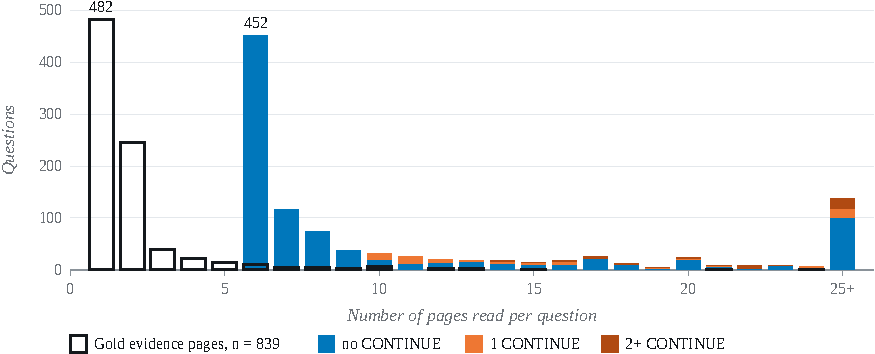
\includegraphics[width=\textwidth]{method/method_trajectory_v2.pdf}
    \caption{Pages read by the proposed pipeline compared with the number of annotated gold evidence pages. Trajectories are separated by the number of times the \texttt{arbiter} requests further evidence acquisition.}
    \label{fig:method_trajectory}
\end{figure}

\paragraph{Adaptive evidence acquisition.}
Figure~\ref{fig:method_trajectory} shows that the pipeline does not consume a fixed page budget for every question. The largest group terminates after six pages, the minimum initial reading depth, while progressively fewer questions continue further through the ranked document and a smaller tail reads 25 or more pages. Reopened trajectories account for part of this tail, with some questions requiring additional reading after an initial synthesis attempt. This behaviour is closely tied to retriever quality: when relevant pages are ranked early, sufficient evidence can be collected quickly and the \texttt{reader} can terminate near the minimum depth; when evidence is poorly ranked or distributed across several pages, deeper traversal becomes necessary. Adaptive acquisition therefore shifts compute toward questions whose evidence is harder to recover rather than assigning the same context budget to every query.

% GENERATED by tables/scripts/method_cost.py -- do not edit by hand, re-run the script.
% Numbers read from results/method/telemetry_v5/per_turn_by_role.csv and per_question_summary.csv,
% written by `python -m seqread.build --iteration 5`.
\begin{table}[ht]
\centering
\small
\setlength{\tabcolsep}{5pt}
\renewcommand{\arraystretch}{1.12}
\adjustbox{max width=\textwidth}{%
\begin{tabular}{@{}l r rrr rr r@{}}
\toprule
& & \multicolumn{3}{c}{\textbf{Tokens}} & \multicolumn{2}{c}{\textbf{Latency (s)}} & \textbf{Peak} \\
\cmidrule(lr){3-5}\cmidrule(lr){6-7}
& \textbf{Turns} & \textbf{Input text} & \textbf{Input visual} & \textbf{Output} & \textbf{Prefill} & \textbf{Decode} & \textbf{VRAM (GiB)} \\
\midrule
\texttt{reader} & 11.2 & 5{,}209 & 834 & 1{,}008 & 2.0 & 70.6 & 7.3 \\
\texttt{synthesizer} & 1.4 & 9{,}638 & 1{,}742 & 724 & 4.0 & 59.0 & 8.2 \\
\texttt{arbiter} & 1.3 & 4{,}988 & 0 & 1{,}083 & 1.6 & 72.8 & 7.1 \\
\midrule
Per question, mean & 13.9 & 78{,}215 & 11{,}733 & 13{,}721 & 29.7 & 968.1 & 8.2 \\
Per question, median & 9.0 & 37{,}484 & 7{,}272 & 8{,}081 & 13.8 & 544.6 & 8.0 \\
\bottomrule
\end{tabular}%
}
\caption{Inference cost of the pipeline per agent turn and question.} % Over the 1{,}069 MMLongBench-Doc questions the pipeline finished, role rows give the mean per agent turn, with \textbf{Turns} the mean number of that role's turns per question; the per-question rows give each question's totals, with peak VRAM its highest turn. Every turn counts its completion passes. Visual tokens are those the language model receives after Qwen3-VL's patch merge. A question takes 16.6 minutes on average (median 9.4), almost all of it decoding, and no turn exceeds 13.4\,GiB.}
\label{tab:method_cost}
\end{table}

\paragraph{Inference cost.}
Table~\ref{tab:method_cost} shows that the pipeline averages 13.0 role turns per question, with most computation spent in the \texttt{reader}. Mean peak memory is only 8.4\,GiB, keeping the system comfortably within the 16\,GB deployment budget, but repeated sequential decoding makes latency the principal cost, with an average runtime of approximately 10.7 minutes per question. The method therefore trades low memory use for additional sequential inference and broader adaptive evidence acquisition.

\paragraph{Limitations.}
The deliberately simple design leaves several clear weaknesses. LongDocURL localisation tasks require the system to map topic descriptions or paragraph summaries to exact section titles, identify named tables from descriptions, or jointly interpret figures and tables. Our pipeline is not explicitly designed for this kind of structured localisation: it follows a fixed page ranking, stores free-form evidence records, and has no section-aware indexing, table-level retrieval, or mechanism for matching descriptions against document structure. Multi-page reasoning remains difficult for a related reason. Evidence from most inspected pages is compressed into \texttt{reader} records, leaving the \texttt{synthesizer} to combine these summaries with a smaller set of flagged pages in a single reasoning step. More sophisticated extensions could incorporate structure-aware retrieval over section titles and tables, finer-grained evidence units, relation-aware navigation, or hierarchical cross-page reasoning. These are left for future work, since the present method is intended primarily as a proof of concept that the preceding design findings can already support a competitive system with a deliberately simple pipeline.

\section{Open Challenges and Future Work}
\label{sec:conc_challenges}

The survey of Chapter~\ref{ch:survey} identifies five challenges that define the open MP-VRDU frontier. They arise from a consistent pattern across the surveyed systems: progress comes from moving evidence handling out of the backbone through compression, retrieval, or iterative orchestration, but each shift relocates the bottleneck rather than removing it. Three challenges concern system capability, namely the evidence pipeline, faithfulness, and efficiency, while two concern data and evaluation, namely supervision integrity and evaluation scope.

\subsection{Evidence Pipeline Bottleneck}
\label{sec:conc_pipeline}

MP-VRDU systems must reconcile high-resolution per-page reading with document-scale evidence aggregation, an objective that exceeds any MLLM's compute and context budget~\citep{ma2024mmlongbench}. Every architectural family takes a lossy compromise. Compression can discard fine-grained content and is typically fixed before the question is seen. Retrieval bounds answer accuracy when required evidence is missed, while broader retrieval can introduce distracting context and attention dilution. Iterative retrieval can recover from some initial misses, but still inherits the limitations of the retrievers, parsers, and other tools it invokes. Cross-page structure compounds the problem further, since none of the approaches in \S\ref{sec:modality-structure} scales cleanly. Future work should explore query-conditional compression, retrieval that follows cross-references and logical relations, and learned cross-page structural representations.

\subsection{Faithfulness and Abstention}
\label{sec:conc_faithfulness}

Long documents amplify hallucination risk. When retrieval misses the answer-bearing region or compression discards it, current systems may still produce confident answers. Few surveyed systems support abstention, calibrated uncertainty, or citation-grounded generation, leaving users with limited signals for distinguishing supported answers from unsupported ones. Future work should integrate evidence-grounded decoding, learned abstention for unanswerable or unretrievable questions, and trajectory-level faithfulness audits that verify whether the evidence used by the system actually supports the final answer.

\subsection{Efficiency and Deployability}
\label{sec:conc_efficiency}

Agentic and retrieval-augmented pipelines can issue many model calls per question, with token and latency costs scaling with both document length and trajectory depth. The surveyed literature reports comparatively little inference-cost analysis: end-to-end latency, token budgets per query, memory requirements, and accuracy--cost trade-offs are often absent despite their importance for practical deployment. Future work should treat compute as a first-class evaluation axis, develop efficient inference techniques for long documents such as cross-round caching, speculative decoding, and adaptive depth, and explore compact MP-VRDU models~\citep{hannan2026docslm} that operate under realistic on-device or privacy constraints.

\subsection{Supervision Scarcity and Contamination}
\label{sec:conc_supervision}

Per-page annotation does not scale to documents averaging tens of pages, so most systems rely on LVLM-synthesised QA over scraped PDFs~\citep{tanaka2024instructdoc,jain2025simpledoc,xiong2026docr1,zhang2026docdancer}. Compounding this, benchmark construction often reuses documents from earlier suites: MMLongBench-Doc draws documents from DUDE, SlideVQA, and ChartQA~\citep{ma2024mmlongbench}, while MP-DocVQA is built on DocVQA~\citep{tito2023hierarchical,mathew2021docvqa}. Together, MLLM-generated QA data~\citep{deng2025longdocurl} and benchmark-reused fine-tuning sets~\citep{xiong2026docr1,duan2025docopilot} risk contamination: models may train on benchmark-derived documents and be evaluated on overlapping data, sometimes judged by the same MLLM family. Future work should adopt held-out documents, declare cross-suite overlap, and separate generators from evaluators.

\subsection{Evaluation Methodology and Scope}
\label{sec:conc_evaluation}

Beyond contamination, two further evaluation gaps persist. Answer-only accuracy masks retrieval failure and rewards correct answers reached through incorrect reasoning. Newer benchmarks score retrieval and page-localisation alongside VQA-style answers~\citep{hui2024uda,zhu2026doclens}, but the practice is not yet standardised, and adaptive pipelines can produce variable trajectories that further complicate reproducibility. Task, language, and domain scope also remain narrow. Real-world MP-VRDU spans summarisation and structured extraction beyond VQA, multilingual layouts beyond English, and domain-specialised settings such as medical, legal, and financial documents, as well as streaming inputs that arrive page-by-page. These dimensions are inherited from SP-VRDU~\citep{ding2026survey} rather than introduced by the multi-page setting and remain underexplored in both regimes. Future work should therefore standardise trajectory-level evaluation with retrieval and grounding metrics, report variability where adaptive inference is used, and broaden coverage along these inherited dimensions.

\section{Concluding Remarks}
\label{sec:concluding_remarks}

The empirical analysis in Chapter~\ref{ch:empirical} partially addresses several of the open challenges identified above. It clarifies where failures arise across representation, selection, and reasoning, examines the trade-off between supported answering and abstention, and characterises how design choices such as retrieval depth, model scale, and numerical precision affect both accuracy and deployment cost. These results do not fully resolve the broader challenges in evidence handling, faithfulness, or efficiency, but provide more concrete guidance for navigating them. Section~\ref{sec:simple_method} then offers a limited system-level validation by showing that these findings can be combined into a deliberately simple competitive pipeline.

More broadly, this thesis contributes three complementary views of MP-VRDU: a survey that organises the design space through an evidence-management perspective, an empirical framework for locating failure within that space, and a working system that translates those findings into practice. Together, these contributions provide a clearer account of how modern MP-VRDU systems are built, where they fail, and how those failures can inform subsequent design.

\section*{Word Count and Appendices}
The main text is approximately 16{,}500 words, excluding the abstract, acknowledgements, tables, captions, and the appendix. The appendix contains supplementary detail including the full survey methodology, surveyed corpus details, extended result tables and full method details; these not essential for reading this thesis.

\section*{Statement of LLM Use}
LLM assistants were used to correct grammatical inaccuracies and suggest phrasing revisions in the manuscript and to assist with implementation of the experimental pipeline. All generated code was read and tested by the author and the author takes full responsibility for the content of this thesis. LLM assistants did not participate in research ideation.

\section*{Additional Artefacts}
\begin{itemize}
    % \item Survey (Chapter~\ref{ch:survey}), ACL Anthology: \url{https://aclanthology.org/PLACEHOLDER}
    \item Survey code and surveyed corpus: \url{https://github.com/LeweiXu/MP-VRDU-Survey}
    % \item Empirical attribution (Chapter~\ref{ch:empirical}), arXiv: \url{https://arxiv.org/abs/PLACEHOLDER}
    \item Empirical attribution and method code: \url{https://github.com/LeweiXu/MP-VRDU-Analysis}
    \item Original project proposal: \url{https://www.overleaf.com/read/ntdnhjhxkgqt#386d92}
\end{itemize}


% ============================================================================
%  References
% ============================================================================
\unnumberedchapter{References}
\bibliography{survey/custom, empirical/custom, include/custom}

% ============================================================================
%  Appendices
% ============================================================================
\appendix
%  \appendix switches \chaptertitlename to "Appendix" and the numbering to
%  letters, so these render as "Appendix A / Title" in the same style as the
%  chapters.

% \chapter{Additional Thesis Details}
% \clearpage

\chapter{Additional Survey Details}

\section{Comparison with Prior Surveys}
\label{app:survey-comparison}
\begin{table*}[h]
\centering
\setstretch{1}
\footnotesize
\setlength{\tabcolsep}{5pt}
\renewcommand{\arraystretch}{1.15}
\newcolumntype{L}[1]{>{\raggedright\arraybackslash\hsize=#1\hsize}X}
\begin{tabularx}{\textwidth}{@{}L{1.75} L{0.5} L{1.0} L{0.75} L{1.0}@{}}
\toprule
\textbf{Survey} & \textbf{Venue} & \textbf{Scope} & \textbf{Multi-Page Treatment} & \textbf{Organising Framing} \\
\midrule
A Survey of Deep Learning Approaches for OCR and Document Understanding~\citeauthor{subramani2020survey} & arXiv 2020 & Pre-MLLM OCR pipelines & Not covered & Pipeline stage (detection, recognition, layout) \\
Deep Learning Approaches for Information Extraction from Visually Rich Documents: Datasets, Challenges and Methods~\citeauthor{gbada2025deep} & IJDAR 2025 & Information extraction over VRDs & Not covered & Extraction task and method \\
Deep Learning based Visually Rich Document Content Understanding: A Survey~\citeauthor{ding2026deep} & AI Review 2026 & Content understanding over VRDs & Not covered & Task formulation, architecture, pretraining \\
A Survey on MLLM-based Visually Rich Document Understanding: Methods, Challenges, and Emerging Trends~\citeauthor{ding2026survey} & ACL 2026 & MLLM-era VRDU & In passing & OCR dependency; architecture, training, benchmarks \\
Scaling Beyond Context: A Survey of Multimodal Retrieval-Augmented Generation for Document Understanding~\citeauthor{gao2026scaling} & ACL 2026 & Multimodal RAG for long documents & Partial (RAG techniques only) & Retrieval-augmented generation \\
\midrule
\textbf{This survey} & EMNLP 2026 & \textbf{Multi-page VRDU} & \textbf{Distinct problem} & \textbf{Evidence management} \\
\bottomrule
\end{tabularx}
\caption{Comparison of this survey with prior VRDU surveys. Prior surveys either predate the multi-page literature or address it only within a broader single-page or extraction-focused scope. This survey is the first to treat multi-page VRDU as a distinct problem organised around evidence management.}
\label{tab:survey-comparison}
\end{table*}

Table~\ref{tab:survey-comparison} contrasts this survey with the five prior VRDU surveys closest to our scope. The comparison is along three axes. \textbf{Scope} records the era and problem each survey targets, from pre-MLLM OCR pipelines to the recent MLLM and retrieval-augmented literature. \textbf{Multi-page treatment} records whether multi-page understanding is treated as a distinct problem with its own design axes, addressed only in passing within a broader scope, or left out. \textbf{Organising framing} records the lens each survey uses to structure the field. Prior surveys either predate the multi-page literature or treat it as one topic within a single-page or extraction-focused scope. This survey is the first to define MP-VRDU as a distinct problem, to organise it around evidence management, and to cover the four architectural families, modality pressures, inference-time and training strategies, and datasets specific to the multi-page setting.

\section{Full Survey Methodology}
\label{app:sv_methodology}

\subsection{Search keywords.}
Queries combined a multi-page cluster with a task or method cluster. Multi-page terms included ``multi-page document'', ``long document'', ``long-context document'', ``cross-page reasoning'', ``page-level retrieval'', ``document-scale evidence'', and ``hundred-page''. Task and method terms included ``document visual question answering'', ``visually rich document understanding'', ``document VQA'', ``document agent'', ``visual document retrieval'', ``document RAG'', ``hierarchical document transformer'', and ``long-context vision-language model''. Benchmark-name probes (``MP-DocVQA'', ``MMLongBench-Doc'', ``LongDocURL'', ``DUDE'', ``SlideVQA'', ``M3DocVQA'', ``DocBench'', ``M-LongDoc'') were used as anchors for forward-citation sweeps to capture systems that report against multi-page evaluation suites.

\subsection{Inclusion and exclusion criteria.}
A paper was retained if it (i) proposed a multi-page model, framework, system, or pipeline rather than a benchmark or dataset alone, and (ii) reported quantitative results on at least one multi-page benchmark, with cross-page evidence handling as an explicit design contribution. Excluded categories were single-page-only systems benchmarked solely on DocVQA, InfographicVQA, ChartQA, FUNSD, or CORD; survey, position, and opinion papers; generic OCR or table-extraction tools without VQA or reasoning evaluation; long-context LLM benchmarks where documents are one input type among many; and dataset-only contributions, which are catalogued separately in \S\ref{sec:datasets}. Peer-reviewed venue publications and arXiv preprints were assessed against the same substantive criteria, since recent MP-VRDU progress has appeared predominantly in preprint form; venue status is recorded per entry in Table~\ref{tab:model_survey_arch}. Table~\ref{tab:survey_corpus} lists the surveyed systems grouped by architectural family, with the multi-page contribution on which each was included.

\subsection{Knowledge extraction and verification.}
Each retained paper was converted to markdown and processed through LLM-assisted key-information extraction with evidence-span location, populating per-model fields covering architectural family, OCR dependency, vision encoder, LLM backbone, adaptors and projectors, page-rendering resolution, training stages, datasets used per stage, and reported scores on each benchmark. Every extracted field was manually verified against the source paper before being added.

\subsection{Dataset catalogue.}
The dataset catalogue in \S\ref{sec:datasets} was built primarily from the pretraining, fine-tuning, and benchmarking datasets named by every paper in the surveyed corpus, supplemented with a small set of datasets the corpus does not yet adopt but that cover MP-VRDU-relevant settings such as long scientific documents, multi-page tables, and cross-page reasoning suites, included to surface datasets whose adoption may strengthen future cross-system comparison.

\begin{table*}[p]
\centering
% The document runs at \setstretch{1.1}. A 50-row table does not need that extra
% leading, and giving it back is most of what makes this fit on one page.
\setstretch{1}
\scriptsize
\captionsetup{font=small}
% A wider description column is what actually buys the page: at 0.74 most rows
% wrap to two lines, at 0.78 most do not, which is worth ~140pt of height. The
% table then overruns \textwidth by 6%, and the adjustbox below scales that back.
\setlength{\tabcolsep}{3pt}
\renewcommand{\arraystretch}{1.0}
% Defined here as well as in survey/models_summary.tex, so this table does not
% depend on that one having been input first.
\definecolor{sectionbg}{gray}{0.88}
% Backstop: only scales if the rows still overrun, and leaves the caption alone.
\begin{adjustbox}{max totalsize={\textwidth}{0.93\textheight},center}
\begin{tabular}{@{}l l >{\raggedright\arraybackslash}p{0.78\textwidth}@{}}
\toprule
\textbf{Model} & \textbf{Venue} & \textbf{Multi-Page Contribution} \\
\midrule

\rowcolor{sectionbg}
\multicolumn{3}{l}{\textbf{Page-to-Document Encoding Models}} \\
\midrule
  {Arctic-TILT}~(\citeyear{borchmann2025arctic}) & ACL & Layer-wise tensor-product text-image fusion with chunked sparse attention, serving up to 389k tokens on a single GPU \\
  {GRAM}~(\citeyear{blau2024gram}) & CVPR & Interleaves page-level and document-level attention sub-layers with learnable global Doc tokens, avoiding quadratic concatenation cost \\
  {Hi-VT5}~(\citeyear{tito2023hierarchical}) & PR & Learnable [PAGE] tokens summarise each page; decoder consumes the concatenated page tokens, with answer-page prediction for explainability \\
  {RM-T5}~(\citeyear{dong2024multi}) & DAS & Recurrent memory tokens propagate context page-by-page; per-page memories concatenated for decoding \\

\midrule[0.4pt]

\rowcolor{sectionbg}
\multicolumn{3}{l}{\textbf{MLLM-Centric Adaptation Models}} \\
\midrule
  {CoR}~(\citeyear{guo2026end}) & preprint & Four-stage Chain-of-Reading paradigm with a caption-reconstruction objective for figure and table grounding \\
  {Docopilot}~(\citeyear{duan2025docopilot}) & CVPR & Native multi-page MLLM trained on Doc-750K cross-page proxy tasks with context-extension engineering \\
  {DocR1}~(\citeyear{xiong2026docr1}) & AAAI & EviGRPO adds an evidence-page F1 reward over structured think/evidence/answer outputs \\
  {DocSeeker}~(\citeyear{yan2026docseeker}) & CVPR & Analysis-Localization-Reasoning paradigm with page-identifier grounding and evidence-guided resolution allocation \\
  {DocSLM}~(\citeyear{hannan2026docslm}) & CVPR & Hierarchical compressor fixes 576 tokens per page; streaming segments with entropy-based abstention for edge deployment \\
  {InstructDoc}~(\citeyear{tanaka2024instructdoc}) & AAAI & Document-former fuses OCR, layout, and visual features into learnable tokens, with pages encoded in parallel \\
  {LayTokenLLM}~(\citeyear{zhu2025simple}) & CVPR & Per-segment layout token shares its segment's position ID, adding layout without consuming context \\
  {Leopard}~(\citeyear{jia2025leopard}) & TMLR & Adaptive high-resolution multi-image encoding under a global token budget with pixel-shuffle compression \\
  {mPLUG-DocOwl2}~(\citeyear{hu2025mplug}) & ACL & DocCompressor cross-attends global low-resolution queries to sub-image features, compressing each page to 324 tokens \\
  {Texthawk2}~(\citeyear{yu2024texthawk2}) & preprint & Two-step resampling and rearrangement for 16$\times$ visual-token compression with a coordinate-token detection head \\
  {URaG}~(\citeyear{shi2026urag}) & AAAI & Cross-modal retrieval module at an early Transformer layer discards non-retained pages before deeper layers \\

\midrule[0.4pt]

\rowcolor{sectionbg}
\multicolumn{3}{l}{\textbf{Retrieval-Augmented Pipelines}} \\
\midrule
  {AVIR}~(\citeyear{li2026avir}) & MMAsia & Adaptive page selector uses score-distribution clustering to set per-query retrieval depth \\
  {CREAM}~(\citeyear{zhang2024cream}) & ACM & Coarse-to-fine retrieval with iterative reranking, paired with attention-pooled multi-page visual features \\
  {DFVC}~(\citeyear{qian2026accurate}) & MDPI & Adapter predicts gating weights over neighbouring-page embeddings to fuse cross-page context into page representations \\
  {DREAM}~(\citeyear{zhang2025dream}) & MM & Learning-to-rank fusion of embedding similarity and keyword-guided MLLM scores, with cross-page mixture-of-experts routing \\
  {KGP}~(\citeyear{wang2024knowledge}) & AAAI & Knowledge graph over passage and structural nodes traversed by an LLM agent to gather supporting facts \\
  {M2RAG}~(\citeyear{duan2025m2rag}) & NeurIPS & Dual-tower sparse and dense retrieval with text, visual, and fusion agents performing consistency checking \\
  {M3DocRAG}~(\citeyear{cho2024m3docrag}) & preprint & ColPali late-interaction page retrieval with approximate indexing, scaling to 40k+ pages \\
  {MDocAgent}~(\citeyear{han2025mdocagent}) & preprint & Five-stage pipeline with parallel text and image retrieval and specialised modality agents \\
  {MHier-RAG}~(\citeyear{gong2026mhier}) & preprint & Combines flattened in-page indexing with a recursively summarised cross-page tree for multi-granularity retrieval \\
  {MLDocRAG}~(\citeyear{zhang2026mldocrag}) & preprint & Chunk-Query Graph of LVLM-generated queries links chunks for retrieval by query-to-query similarity \\
  {MM-R5}~(\citeyear{xu2025mm}) & AAAI & Two-stage reranker training with structured reasoning chains and rank-discounted GRPO rewards \\
  {MoLoRAG}~(\citeyear{wu2025molorag}) & EMNLP & Traverses a page graph combining semantic and VLM-judged logical relevance to reach weakly-similar evidence \\
  {MultiDocFusion}~(\citeyear{shin2026multidocfusion}) & ACL & LLM-constructed document hierarchy tree drives depth-first hierarchical chunking \\
  {PDF-WuKong}~(\citeyear{xie2026pdf}) & IJCV & End-to-end sparse sampler jointly trained with the LLM selects top-K text and image evidence \\
  {RAG-DocVQA}~(\citeyear{pez2025enhancing}) & ICDAR & Systematic comparison of textual and visual RAG variants for multi-page DocVQA \\
  {Self-Attention Scoring}~(\citeyear{kang2024multi}) & ICDAR & Self-attention scoring module ranks independently encoded pages, extending evaluation to 793-page documents \\
  {SLEUTH}~(\citeyear{liu2025resolving}) & CVPR & Training-free clue discovery and page screening keep effective context fixed as retrieval depth grows \\
  {SV-RAG}~(\citeyear{chen2025sv}) & ICLR & Dual LoRA adapters over one MLLM backbone serve both late-interaction page retrieval and answering \\
  {VDocRAG}~(\citeyear{tanaka2025vdocrag}) & CVPR & Compresses each page image to a single dense embedding via self-supervised compression pretraining tasks \\
  {VisDoMRAG}~(\citeyear{suri2025visdom}) & NAACL & Parallel textual and visual RAG chains reconciled by consistency-constrained modality fusion \\

\midrule[0.4pt]

\rowcolor{sectionbg}
\multicolumn{3}{l}{\textbf{Adaptive-Trajectory Pipelines}} \\
\midrule
  {DMAP}~(\citeyear{fu2026dmap}) & WWW & Hierarchical document map traversed by tri-path retrieval with a reflective loop for insufficient evidence \\
  {Doc-V*}~(\citeyear{zheng2026doc}) & ACL & Thumbnail overview then alternating retrieval and high-resolution page fetch, trained by SFT then GRPO \\
  {DocAgent}~(\citeyear{sun2025docagent}) & EMNLP & Hierarchical XML outline navigated by an actor agent with five tools, plus a reviewer and persistent memory bank \\
  {DocDancer}~(\citeyear{zhang2026docdancer}) & preprint & End-to-end trained agent with only search and read tools, learned from synthesised exploration trajectories \\
  {DocLens}~(\citeyear{zhu2026doclens}) & ACL & Page navigator and element localiser zoom to fine-grained evidence; sampling-adjudication selects among candidates \\
  {DocReact}~(\citeyear{wu2025doc}) & ACL & Frames iterative retrieval as information-gain maximisation, halting when residual entropy stops decreasing \\
  {MACT}~(\citeyear{yu2025visual}) & preprint & Four specialised agents with independent judgment routing and agent-wise adaptive test-time scaling \\
  {MM-Doc-R1}~(\citeyear{lin2026mm}) & ACL & Planner-seeker-answer workflow trained by similarity-weighted policy optimisation for multi-turn RL \\
  {SimpleDoc}~(\citeyear{jain2025simpledoc}) & EMNLP & Dual-cue retrieval over embeddings and page summaries, with a memory-carrying reasoner that reissues refined queries \\
  {ViDoRAG}~(\citeyear{wang2025vidorag}) & EMNLP & Gaussian-mixture adaptive top-K retrieval with seeker, inspector, and answer agents over multi-scale views \\
  {VRAG-RL}~(\citeyear{wang2025vrag}) & NeurIPS & Visual perception action space lets the agent crop and zoom regions, trained with retrieval-efficiency rewards \\

\bottomrule
\end{tabular}
\end{adjustbox}
\caption{The 46 surveyed MP-VRDU systems. Grouped by architectural family, with the multi-page contribution motivating each system's inclusion. Venue indicates the publication venue at time of writing.}
\label{tab:survey_corpus}
\end{table*}

\section{Additional Resources}

\subsection{Reported Performance by Architecture}
\label{app:performance}

% ─────────────────────────────────────────────────────────────────────────────
% Auto-generated by performance_tables_convert.py — do NOT edit manually.
% Re-generate:  python3 performance_tables_convert.py model_performance.csv model_performance
%
% Required packages (add to your preamble):
%   \usepackage{booktabs}
%   \usepackage{array}
%   \usepackage{xcolor}
%   \usepackage{colortbl}
%   \usepackage{caption}
%   \usepackage{adjustbox}
% ─────────────────────────────────────────────────────────────────────────────

\definecolor{sectionbg}{gray}{0.88}

% ── tab:model_performance_arch ──────────────────────────────────────────────────────────────
\begin{table*}[!h]
\centering
\scriptsize
\captionsetup{font=small}
\setlength{\tabcolsep}{2.5pt}
\renewcommand{\arraystretch}{0.86}
\begin{adjustbox}{width=\textwidth}
\begin{tabular}{l l c c c c c c c}
\toprule
 &  & \multicolumn{1}{c}{\textbf{MP-DocVQA}} & \multicolumn{1}{c}{\textbf{DUDE}} & \multicolumn{1}{c}{\textbf{LongDocURL}} & \multicolumn{2}{c}{\textbf{MMLongBench-Doc}} & \multicolumn{2}{c}{\textbf{SlideVQA}} \\
\cmidrule(lr){3-3}\cmidrule(lr){4-4}\cmidrule(lr){5-5}\cmidrule(lr){6-7}\cmidrule(lr){8-9}
\textbf{Model} & \textbf{Variant} & \textbf{ANLS} & \textbf{ANLS} & \textbf{Accuracy} & \textbf{Accuracy} & \textbf{F1} & \textbf{EM} & \textbf{F1} \\
\midrule

% ── General Domain MLLM ─────────────────────────────────────────────────────────────
\rowcolor{sectionbg}
\multicolumn{9}{l}{\textbf{General Domain MLLM}} \\
\midrule
  Claude-3-Opus & Claude-3-Opus & -- & -- & -- & 17.4 & 18.1 & -- & -- \\
  Gemini-1.5-Pro & Gemini-1.5-Pro & -- & -- & 50.9 & 28.2 & 20.6 & -- & -- \\
  GPT-4o & GPT-4o (LVLM mode) & -- & -- & 64.5 & 42.8 & 44.9 & -- & -- \\
  GPT-4V & GPT-4V(ision) & -- & -- & -- & 32.4 & 31.2 & -- & -- \\
  InternVL-Chat-v1.5 & InternVL-Chat-v1.5-26B & -- & -- & -- & 14.6 & 13.0 & -- & -- \\
  LLaVA-OneVision-7B & LLaVA-OneVision-Chat-7B & -- & -- & 25.0 & -- & -- & -- & -- \\
  MiniCPM-Llama3-V2.5-8B & MiniCPM-Llama3-V2.5 & -- & -- & -- & 8.5 & 8.6 & -- & -- \\
  Qwen2-VL-7B & Qwen2-VL-7B & -- & -- & 30.6 & -- & -- & -- & -- \\

\midrule[0.4pt]

% ── Page-to-Document Encoding Models ─────────────────────────────────────────────────────────────
\rowcolor{sectionbg}
\multicolumn{9}{l}{\textbf{Page-to-Document Encoding Models}} \\
\midrule
  Arctic-TILT & Arctic-TILT & 81.2 & 58.1 & -- & 25.8 & -- & 55.1 & -- \\
  GRAM & GRAM-859M & 80.32 & 51.15 & -- & -- & -- & -- & -- \\
  Hi-VT5 & Hi-VT5 (multipage) & 62.01 & -- & -- & -- & -- & -- & -- \\
  RM-T5 & RM-T5 & 64.01 & -- & -- & -- & -- & -- & -- \\

\midrule[0.4pt]

% ── MLLM-Centric Adaptation Models ─────────────────────────────────────────────────────────────
\rowcolor{sectionbg}
\multicolumn{9}{l}{\textbf{MLLM-Centric Adaptation Models}} \\
\midrule
  DocR1 & DocR1 & 87.45 & 54.39 & -- & -- & -- & -- & 71.96 \\
  DocSeeker & DocSeeker (full SFT + EviGRPO) & 86.2 & 57.4 & 51.7 & 40.1 & -- & -- & 77.1 \\
  Leopard & Leopard-LLaVA-Pro & 70.6 & 43.82 & -- & -- & -- & -- & 37.51 \\
  mPLUG-DocOwl2 & DocOwl2-8B & 69.42 & 46.77 & -- & -- & -- & -- & -- \\
  URaG & URaG-7B & 88.2 & 57.6 & 52.2 & 33.8 & 32.8 & 72.1 & -- \\
  Docopilot & Docopilot-8B & 81.3 & -- & -- & 28.8 & 23 & -- & -- \\
  Texthawk2 & Texthawk2 & -- & -- & -- & -- & -- & -- & -- \\
  DocSLM & DocSLM-2B & 70 & 47.6 & -- & -- & -- & -- & -- \\
  InstructDoc & InstructDoc (finetuned) & -- & 46.8 & -- & -- & -- & 37.7 & 47.3 \\
  LayTokenLLM & LayTokenLLM-8B & 74.31 & 52 & -- & -- & -- & -- & -- \\
  CoR & Qwen2.5-VL-CoR-7B & -- & -- & 51.5 & 37.4 & 36 & -- & -- \\

\midrule[0.4pt]

% ── Retrieval-Augmented Pipelines ─────────────────────────────────────────────────────────────
\rowcolor{sectionbg}
\multicolumn{9}{l}{\textbf{Retrieval-Augmented Pipelines}} \\
\midrule
  AVIR & AVIR & 84.58 & -- & -- & -- & -- & 60.3 & 68.9 \\
  DFVC & DFVC (ColQwen backbone) & -- & -- & -- & -- & -- & -- & -- \\
  DREAM & DREAM† (InternVL2-4B + retrieved text) & 85.72 & 52.14 & -- & 27.3 & 28.6 & -- & -- \\
  M3DocRAG & M3DOCRAG (ColPali + Qwen2-VL 7B) & 84.44 & -- & -- & 21 & 22.6 & -- & -- \\
  MM-R5 & MM-R5 (Qwen2.5-VL-7B SFT+GRPO) & -- & -- & -- & -- & -- & -- & -- \\
  MoLoRAG & MoLoRAG+ (Qwen2.5-VL-7B) & -- & -- & 51.85 & 41.01 & -- & -- & -- \\
  Self-Attention Scoring & Pix2Struct-SA proposed & 61.99 & -- & -- & -- & -- & -- & -- \\
  SLEUTH & SLEUTH (Qwen3-VL-8B + ColPali Top-5) & -- & -- & 59.96 & 52.77 & -- & -- & -- \\
  SV-RAG & SV-RAG-InternVL2† R5 (4B) & 71.0 & 45.0 & -- & 23.0 & 24.2 & 31.98 & -- \\
  VDocRAG & VDocRAG & -- & 44 & -- & -- & -- & -- & 42 \\
  CREAM & CREAM & 65.32 & 52.46 & -- & -- & -- & -- & -- \\
  MHier-RAG & MHier-RAG (Qwen-turbo) & -- & -- & 55.7 & 52.3 & 46 & -- & -- \\
  MLDocRAG & MLDocRAG & -- & -- & 50.8 & 47.9 & -- & -- & -- \\
  MultiDocFusion & MultiDocFusion & -- & -- & -- & -- & -- & -- & -- \\
  M2RAG & M[2]RAG top-5 & -- & -- & 57.68 & 39.9 & -- & -- & -- \\
  MDocAgent & MDocAgent (top-4) & -- & -- & 57.8 & 31.5 & -- & -- & -- \\
  PDF-WuKong & PDF-WuKong & 76.9 & 56.1 & -- & -- & -- & -- & -- \\
  RAG-DocVQA & RAG-Qwen2.5-VL & 73.7 & 39.9 & -- & -- & -- & -- & -- \\
  VisDoMRAG & VisDoMRAG (ChatGPT-4o + ColPali + BGE) & -- & -- & -- & -- & -- & -- & 67.22 \\
  KGP & KGP & -- & -- & -- & -- & -- & -- & -- \\

\midrule[0.4pt]

% ── Adaptive-Trajectory Pipelines ─────────────────────────────────────────────────────────────
\rowcolor{sectionbg}
\multicolumn{9}{l}{\textbf{Adaptive-Trajectory Pipelines}} \\
\midrule
  Doc-V* & Doc-V* (GRPO) & 86.2 & 64.5 & 56.3 & 42.1 & -- & -- & 77.2 \\
  DocReact & DocReact (w/ ColPali) & -- & -- & -- & 38.29 & 38.07 & 54.87 & 55.04 \\
  MACT & MACT-MiMo-VL-Series-28B & -- & 70.8 & -- & -- & 47.4 & -- & 83.9 \\
  VRAG-RL & VRAG-RL (Qwen2.5-VL-7B-Instruct) & -- & -- & -- & -- & -- & -- & -- \\
  DocLens & DocLens (Gemini-2.5-Pro) & -- & -- & -- & 67.6 & -- & -- & -- \\
  DMAP & DMAP Ours-Top4 (GPT-4o backbone) & -- & -- & 60.7 & 43.2 & -- & -- & -- \\
  DocAgent & DocAgent (Claude-3.5-Sonnet) & -- & -- & -- & 57.3 & 54.1 & -- & -- \\
  DocDancer & DocDancer (GPT-5.2) & -- & -- & -- & 57 & 56.8 & -- & -- \\
  MM-Doc-R1 & MM-Doc-R1 (Qwen3-8B + SPO) & -- & -- & -- & 49.7 & 46.1 & -- & -- \\
  SimpleDoc & SimpleDoc (3.5 pages) & -- & -- & 72.3 & 60.58 & -- & -- & -- \\
  ViDoRAG & ViDoRAG & -- & -- & -- & -- & -- & -- & -- \\

\bottomrule
\end{tabular}
\end{adjustbox}
\caption{Performance of MP-VRDU models grouped by architecture category. Reported metrics follow the source papers and are not always directly comparable. `--' indicates not reported.}
\label{tab:model_performance_arch}
\end{table*}


Table~\ref{tab:model_performance_arch} summarises reported scores on the five most-adopted multi-page benchmarks, grouped by architectural family. It is included for coverage rather than ranking. The matrix is sparse and metric conventions diverge across MP-DocVQA, DUDE, LongDocURL, MMLongBench-Doc, and SlideVQA, so scores are not comparable across columns; for the same benchmark, differences in backbone scale, proprietary-LLM dependency, evidence budget, and the training-versus-zero-shot distinction mean that a higher score does not by itself indicate a better architecture. Several of the strongest systems orchestrate closed-source frontier backbones of undisclosed scale, so their scores cannot be attributed to architecture alone. Read with these caveats, the table supports one robust cross-family observation: coverage tracks cost structure, with page-to-document and MLLM-centric systems confined to mid-length benchmarks and selective-evidence families dominating the long-document frontier.

\subsection{General Domain MLLM for MP-VRDU}
\label{app:general-MLLM}
Frontier general-domain MLLMs handle short multi-page inputs well when the document fits in context, but the multi-page setting introduces three pressures absent in single-page VRDU: context-window overrun, attention dilution over sparsely distributed evidence~\cite{liu2024lost}, and a per-page reading fidelity versus whole-document coverage trade-off under a fixed token budget. Table~\ref{tab:model_performance_arch} shows that even the strongest frontier MLLMs trail specialised MP-VRDU systems by a wide margin on MMLongBench-Doc and LongDocURL, motivating the specialised architectures examined in \S\ref{sec:architecture}.

\subsection{Model Components Details}
\label{app:components}
Table~\ref{tab:model_components} lists the concrete components of each surveyed system, organised by architectural family. The four families assemble these parts in characteristically different ways. Page-to-document transformers pair smaller LLM backbones (T5 variants, DocFormerv2) with custom layout-aware projectors. MLLM-centric adaptation models reuse standard vision-language stacks such as Qwen2.5-VL, mPLUG-Owl2, and SigLIP variants, and update only light projection or compression modules. Retriever-augmented pipelines decouple a frozen retriever (ColPali, ColQwen, VisRAG) from a frozen LVLM and train only the scorer, fuser, or reranker. Adaptive-trajectory pipelines mostly orchestrate frozen frontier VLMs, with parameter updates restricted to a few systems that fine-tune the controller via SFT or GRPO.

% ─────────────────────────────────────────────────────────────────────────────
% Auto-generated by components_table_convert.py -- do NOT edit manually.
% Re-generate:  python3 components_table_convert.py
%
% Required packages (add to your preamble):
%   \usepackage{booktabs}
%   \usepackage{array}
%   \usepackage{xcolor}
%   \usepackage{colortbl}
%   \usepackage{caption}
%   \usepackage{longtable}
% ─────────────────────────────────────────────────────────────────────────────

\definecolor{sectionbg}{gray}{0.88}

% -- tab:model_components --
{
\scriptsize
\captionsetup{font=small}
\setlength{\tabcolsep}{4pt}
\renewcommand{\arraystretch}{1.1}
\setlength{\LTleft}{0pt}
\setlength{\LTright}{0pt}
\begin{longtable}{@{}
    >{\raggedright\arraybackslash}p{0.12\textwidth}
    >{\raggedright\arraybackslash}p{0.18\textwidth}
    >{\raggedright\arraybackslash}p{0.18\textwidth}
    >{\raggedright\arraybackslash}p{0.22\textwidth}
    >{\raggedright\arraybackslash}p{0.22\textwidth}
@{}}
\caption[Per-model components of the surveyed MP-VRDU systems.]{Per-model components of the surveyed MP-VRDU systems. Resolution lists the input image resolution or page-rendering setting; \textit{dynamic} denotes encoders that accept variable-resolution input. `--' indicates not reported \ not applicable.} \label{tab:model_components} \\
\toprule
\textbf{Model} & \textbf{Vision Backbone} & \textbf{Resolution} & \textbf{LLM Backbone} & \textbf{Adaptors and Projectors} \\
\midrule
\endfirsthead

\multicolumn{5}{l}{\textit{Table \ref{tab:model_components} -- continued from previous page}} \\
\toprule
\textbf{Model} & \textbf{Vision Backbone} & \textbf{Resolution} & \textbf{LLM Backbone} & \textbf{Adaptors and Projectors} \\
\midrule
\endhead

\midrule \multicolumn{5}{r}{\textit{Continued on next page}} \\
\endfoot

\bottomrule
\endlastfoot

% -- Page-to-Document Encoding Models --
\rowcolor{sectionbg}
\multicolumn{5}{l}{\textbf{Page-to-Document Encoding Models}} \\
\midrule
  Arctic-TILT & U-Net & 400k tokens / 500p & T5-Large & TILT fusion \\
  \arrayrulecolor{black!15}\midrule\arrayrulecolor{black}
  GRAM & DocFormerv2 & 800 tok/page train, 8000 test & DocFormerv2 & -- \\
  \arrayrulecolor{black!15}\midrule\arrayrulecolor{black}
  Hi-VT5 & DiT & 224x224 (DiT default), 20480 max tokens & T5 & -- \\
  \arrayrulecolor{black!15}\midrule\arrayrulecolor{black}
  RM-T5 & DiT & 512 tok/page max & T5-base & -- \\

\midrule[0.4pt]

% -- MLLM-Centric Adaptation Models --
\rowcolor{sectionbg}
\multicolumn{5}{l}{\textbf{MLLM-Centric Adaptation Models}} \\
\midrule
  DocR1 & Qwen2.5-VL & dynamic, max 1024 patches & Qwen2.5-VL-7B & Frozen Qwen MLP projector \\
  \arrayrulecolor{black!15}\midrule\arrayrulecolor{black}
  DocSeeker & Qwen2.5-VL ViT & 1024x784 eval, EGRA training & Qwen2.5-VL-7B-Instruct & -- \\
  \arrayrulecolor{black!15}\midrule\arrayrulecolor{black}
  Leopard & SigLIP-SO400M & 364x364 / 980x980, max 50 sub-imgs & LLaMa-3.1-8B / Mistral-7B & MLP / Idefics2 resampler \\
  \arrayrulecolor{black!15}\midrule\arrayrulecolor{black}
  mPLUG-DocOwl2 & ViT-L/14 & 504x504, max 12 crops & mPLUG-Owl2 & H-Reducer + DocCompressor \\
  \arrayrulecolor{black!15}\midrule\arrayrulecolor{black}
  URaG & Qwen2.5-VL ViT & dynamic & Qwen2.5-VL-3B / Qwen2.5-VL-7B & Cross-modal retrieval module (2 linear + GELU) + LoRA \\
  \arrayrulecolor{black!15}\midrule\arrayrulecolor{black}
  Docopilot & InternViT-300M & 448 tile, max 24 tiles & InternLM2-1.8B / InternLM2.5-7B & 2-layer MLP \\
  \arrayrulecolor{black!15}\midrule\arrayrulecolor{black}
  Texthawk2 & SigLIP-SO400M & 224x224 base, max 72 sub-imgs & Qwen2-7B-Instruct & QPN + ReSA \\
  \arrayrulecolor{black!15}\midrule\arrayrulecolor{black}
  DocSLM & SigLIP2 & dynamic 384-1152, 576 tok/page & Qwen2.5-1.5B & OCR/Vision compressor + MLP \\
  \arrayrulecolor{black!15}\midrule\arrayrulecolor{black}
  InstructDoc & CLIP & 224x224 & FlanT5 / BLIP2 & Doc-former + proj \\
  \arrayrulecolor{black!15}\midrule\arrayrulecolor{black}
  LayTokenLLM & -- & -- & LLaMA3-8B / Qwen1.5-7B & Layout tokenizer + LoRA \\
  \arrayrulecolor{black!15}\midrule\arrayrulecolor{black}
  CoR & Qwen2.5-VL & dynamic, 32k max & Qwen2.5-VL-7B & Frozen Qwen MLP projector + LoRA \\

\midrule[0.4pt]

% -- Retrieval-Augmented Pipelines --
\rowcolor{sectionbg}
\multicolumn{5}{l}{\textbf{Retrieval-Augmented Pipelines}} \\
\midrule
  AVIR & Pix2Struct & dynamic, 768-5120 patches & Qwen2.5-VL-3B-AWQ & Frozen Qwen MLP projector \\
  \arrayrulecolor{black!15}\midrule\arrayrulecolor{black}
  DFVC & VisRAG, ColQwen & dynamic & Qwen2-VL-2B-Instruct & Cross-page MLP \\
  \arrayrulecolor{black!15}\midrule\arrayrulecolor{black}
  DREAM & InternVL2 ViT & 448 tile, max 24 tiles & InternVL2-4B & Cross-page MoE attention connector + LoRA \\
  \arrayrulecolor{black!15}\midrule\arrayrulecolor{black}
  M3DocRAG & ColPali / ColQwen & 144 DPI, \textasciitilde{}1700px wide & Qwen2-VL-7B / InternVL2-8B / Idefics2-8B / Idefics3-8B & -- \\
  \arrayrulecolor{black!15}\midrule\arrayrulecolor{black}
  MM-R5 & Qwen2.5-VL ViT & dynamic & Qwen2.5-VL-7B & -- \\
  \arrayrulecolor{black!15}\midrule\arrayrulecolor{black}
  MoLoRAG & ColPali & 448x448 & Qwen2.5-VL 3B/7B / Deepseek-VL-16B / LlaVa-Next-7B & Frozen base projector \\
  \arrayrulecolor{black!15}\midrule\arrayrulecolor{black}
  Self-Attention Scoring & Pix2Struct & 2048 patches & Pix2Struct & -- \\
  \arrayrulecolor{black!15}\midrule\arrayrulecolor{black}
  SLEUTH & ColPali, Qwen3-VL ViT & 448x448 & Qwen3-VL-8B / GLM-4.1V-Thinking-8B / Gemini-2.5-Flash & -- \\
  \arrayrulecolor{black!15}\midrule\arrayrulecolor{black}
  SV-RAG & InternVL2 / PaliGemma / Phi-3-vision & dynamic (InternVL2 default), 448x448 & InternVL2-4B / PaliGemma-3B / Phi-3-vision-4B & Dual LoRA adapters (retrieval + QA) + Col-projection \\
  \arrayrulecolor{black!15}\midrule\arrayrulecolor{black}
  VDocRAG & Phi3V-4.2B & 336x336 dynamic, up to 1344x1344 & Phi3V-4.2B & LoRA + MLP \\
  \arrayrulecolor{black!15}\midrule\arrayrulecolor{black}
  CREAM & Pix2Struct & 2048 patches & LLaMA2-7B & Attn pooling + MLP + LoRA \\
  \arrayrulecolor{black!15}\midrule\arrayrulecolor{black}
  KGP & -- & -- & T5-large, LLaMa-7B, MDR (RoBERTa), ChatGPT & LoRA \\
  \arrayrulecolor{black!15}\midrule\arrayrulecolor{black}
  MHier-RAG & Qwen-VL-Plus & dynamic & Qwen-VL-Plus / GPT-3-turbo / Qwen-turbo / GPT-4o / DeepSeek-chat / ERNIE-turbo & -- \\
  \arrayrulecolor{black!15}\midrule\arrayrulecolor{black}
  MLDocRAG & LVLM Qwen2.5-VL & dynamic & Qwen2.5-VL-32B-Instruct, Qwen2.5-VL-7B, Qwen2.5-72B & Frozen Qwen MLP projector \\
  \arrayrulecolor{black!15}\midrule\arrayrulecolor{black}
  MultiDocFusion & -- & -- & Mistral-8B / Llama-3.2-3B / Qwen-2.5-3B / Qwen-2.5-7B & LoRA \\
  \arrayrulecolor{black!15}\midrule\arrayrulecolor{black}
  M2RAG & VisRAG-Ret & dynamic & Qwen2.5-7B-Instruct, Qwen2.5-VL-7B-Instruct, Qwen2.5-VL-32B & Frozen Qwen MLP projector + LoRA + modal fuser \\
  \arrayrulecolor{black!15}\midrule\arrayrulecolor{black}
  MDocAgent & ColPali / ColQwen2 & 144 DPI & LLaMA-3.1-8B-Instruct, Qwen2-VL-7B-Instruct & -- \\
  \arrayrulecolor{black!15}\midrule\arrayrulecolor{black}
  PDF-WuKong & IXC2-VL-4KHD & dynamic 336px-4K, max 16 tiles & IXC2-VL-4KHD & Sparse sampler \\
  \arrayrulecolor{black!15}\midrule\arrayrulecolor{black}
  RAG-DocVQA & DiT / Pix2Struct & 2048 patches & VT5 / Qwen2.5-VL-7B-Instruct & LoRA \\
  \arrayrulecolor{black!15}\midrule\arrayrulecolor{black}
  VisDoMRAG & ColPali / ColQwen2 & 448x448 (ColPali), dynamic & Qwen2-VL-7B-Instruct / Gemini-1.5-Flash / GPT-4o & -- \\

\midrule[0.4pt]

% -- Adaptive-Trajectory Pipelines --
\rowcolor{sectionbg}
\multicolumn{5}{l}{\textbf{Adaptive-Trajectory Pipelines}} \\
\midrule
  Doc-V* & Qwen2.5-VL ViT & 1024x768 / 256x256 thumb & Qwen2.5-VL-7B-Instruct & Frozen MLP \\
  \arrayrulecolor{black!15}\midrule\arrayrulecolor{black}
  DocReact & ColPali, VisRAG-Ret & 448x448 (ColPali default) / dynamic & GPT-4o & -- \\
  \arrayrulecolor{black!15}\midrule\arrayrulecolor{black}
  MACT & Qwen2.5-VL-7B-Instruct / MiMo-VL-7B-SFT / InternVL3-9B & dynamic & Qwen2.5-VL-7B / MiMo-VL-7B-SFT / InternVL3-9B, Qwen2.5-7B/3B / MiMo-7B-SFT / InternVL3-8B/2B & -- \\
  \arrayrulecolor{black!15}\midrule\arrayrulecolor{black}
  VRAG-RL & Qwen2.5-VL ViT & dynamic & Qwen2.5-VL-3B-Instruct / Qwen2.5-VL-7B-Instruct & -- \\
  \arrayrulecolor{black!15}\midrule\arrayrulecolor{black}
  DocLens & frontier VLMs & dynamic & Gemini-2.5-Pro / Gemini-2.5-Flash / Claude-4-Sonnet & -- \\
  \arrayrulecolor{black!15}\midrule\arrayrulecolor{black}
  DMAP & ColPali & dynamic & GPT-4o / Qwen-plus & -- \\
  \arrayrulecolor{black!15}\midrule\arrayrulecolor{black}
  DocAgent & -- & 144 DPI & Gemini 2.0 Flash / GPT-4o / Claude Sonnet 3.5 & -- \\
  \arrayrulecolor{black!15}\midrule\arrayrulecolor{black}
  DocDancer & Qwen3-VL-235B-A22B-Instruct & 144 DPI & Qwen3-4B/30B-A3B & -- \\
  \arrayrulecolor{black!15}\midrule\arrayrulecolor{black}
  MM-Doc-R1 & Qwen2.5-VL ViT & dynamic & Qwen3-4B / Qwen3-8B & -- \\
  \arrayrulecolor{black!15}\midrule\arrayrulecolor{black}
  SimpleDoc & ColQwen-2.5 & dynamic & Qwen2.5-VL-32B-Instruct, Qwen3-30B-A3B & -- \\
  \arrayrulecolor{black!15}\midrule\arrayrulecolor{black}
  ViDoRAG & Nv-embed-V2, ColQwen2 & dynamic & Qwen2.5-VL / LLaMA3.2-Vision / GPT-4o & -- \\

\end{longtable}
}


\clearpage
\chapter{Additional Attribution Details}

\section{Extended Result Tables}
\label{app:extended_findings}

\subsection{Representation Ladder by Document Domain}
\label{app:ladder_domain}
Table~\ref{tab:ladder_domain_resolution} breaks the representation ladder of Table~\ref{tab:ladder_source} down by document domain, and sweeps the two image-carrying rungs across render resolution. Domain rows partition the pool, so each question is counted exactly once. The ordering of rungs is stable within a row, with TLV winning in six of the seven domains, but variation across domains is considerably wider than variation across rungs: at TLV accuracy ranges from 42.9\% on academic papers to 73.2\% on tutorial and workshop material. Resolution matters most where the image is the only channel, with pooled accuracy at V rising 12.4 points from low to high against 5.5 points at TLV, and the largest gains falling on the domains dominated by dense tables and figures.
% GENERATED by tables/scripts/ -- do not edit by hand, re-run the script.
% Numbers read from results/tables/mmlongbench/headline_full_pool.csv (the ladder by
% domain), faithfulness_answerable_accuracy.csv (its All row), resolution.csv (the
% low/high wings by domain) and resolution_source.csv (their All row).
% Ladder by document domain at medium resolution, with TLV and V swept across low and
% high. Teal is accuracy on the SAME fixed [14,74] scale as findings/ladder.tex, capped
% at 60%; bold marks each row's winning rung within the medium ladder, ties included.
% The last column is NOT an accuracy: it is V minus TLV at medium, a point difference,
% so it takes its own warm scale over [0,13] points.
\definecolor{accteal}{HTML}{1BAF7A}
\definecolor{recwarm}{HTML}{D95926}
\newcommand{\ldashade}[1]{%
  \pgfmathtruncatemacro{\shadeval}{max(0,min(60,(#1-14)/(74-14)*65))}%
  \edef\tmpcol{accteal!\shadeval}%
  \expandafter\cellcolor\expandafter{\tmpcol}%
}
\newcommand{\ldacell}[1]{\ldashade{#1}#1}
\newcommand{\ldabest}[1]{\ldashade{#1}\textbf{#1}}
\newcommand{\lddshade}[1]{%
  \pgfmathtruncatemacro{\shadeval}{max(0,min(55,(#1-0)/(13-0)*55))}%
  \edef\tmpcol{recwarm!\shadeval}%
  \expandafter\cellcolor\expandafter{\tmpcol}%
}
\newcommand{\lddcell}[1]{\lddshade{#1}$-$#1}
\newcommand{\ldugain}[1]{\lddshade{#1}$+$#1}

\begin{table}[ht]
\centering
\small
\setlength{\tabcolsep}{5pt}
\renewcommand{\arraystretch}{1.12}
\adjustbox{max width=\textwidth}{%
\begin{tabular}{@{} l rrrr @{\hskip 12pt} rr @{\hskip 6pt} rr @{\hskip 14pt} r @{}}
\toprule
 & \multicolumn{4}{c}{\textbf{Ladder @ med (\%)}} & \multicolumn{2}{c}{\textbf{TLV}} & \multicolumn{2}{c}{\textbf{V}} & \\
\cmidrule(lr){2-5}\cmidrule(lr){6-7}\cmidrule(lr){8-9}
\textbf{Domain} & \textbf{T} & \textbf{TL} & \textbf{TLV} & \textbf{V} & \textbf{low} & \textbf{high} & \textbf{low} & \textbf{high} & \textbf{$\Delta$V} \\
\midrule
Academic paper       & \ldacell{36.4}   & \ldacell{33.1}   & \ldabest{42.9}   & \ldacell{33.8}   & \ldacell{37.0}   & \ldacell{46.8}   & \ldacell{19.5}   & \ldacell{38.3}   & \lddcell{9.1} \\
Admin / Industry     & \ldacell{50.0}   & \ldacell{56.2}   & \ldabest{67.2}   & \ldacell{54.7}   & \ldacell{64.1}   & \ldacell{70.3}   & \ldacell{42.2}   & \ldacell{64.1}   & \lddcell{12.5} \\
Brochure             & \ldacell{28.6}   & \ldacell{32.5}   & \ldabest{45.5}   & \ldacell{40.3}   & \ldacell{40.3}   & \ldacell{48.1}   & \ldacell{39.0}   & \ldacell{49.4}   & \lddcell{5.2} \\
Financial report     & \ldacell{49.1}   & \ldabest{52.8}   & \ldacell{51.9}   & \ldacell{38.9}   & \ldacell{54.6}   & \ldacell{53.7}   & \ldacell{21.3}   & \ldacell{46.3}   & \lddcell{13.0} \\
Guidebook            & \ldacell{35.8}   & \ldacell{40.0}   & \ldabest{51.7}   & \ldacell{45.0}   & \ldacell{48.3}   & \ldacell{51.7}   & \ldacell{38.3}   & \ldacell{47.5}   & \lddcell{6.7} \\
Research / Intro     & \ldacell{22.6}   & \ldacell{27.4}   & \ldabest{47.6}   & \ldacell{45.3}   & \ldacell{42.9}   & \ldacell{50.0}   & \ldacell{38.2}   & \ldacell{47.6}   & \lddcell{2.3} \\
Tutorial / Workshop  & \ldacell{14.3}   & \ldacell{48.2}   & \ldabest{73.2}   & \ldacell{67.9}   & \ldacell{71.4}   & \ldacell{74.1}   & \ldacell{74.1}   & \ldacell{70.5}   & \lddcell{5.3} \\
\midrule
\textbf{All}         & \ldacell{31.9}   & \ldacell{38.8}   & \ldabest{52.5}   & \ldacell{45.6}   & \ldacell{49.2}   & \ldacell{54.7}   & \ldacell{37.8}   & \ldacell{50.2}   & \lddcell{6.9} \\
\bottomrule
\end{tabular}%
}
\caption{\small Representation ladder by document domain and render resolution. Teal deepens with accuracy and bold marks each row's winning rung; the warm strip deepens with how far vision alone falls below the combined rung. Resolution lifts the domains whose evidence is pixel-limited and leaves the text-heavy ones where they were.}
\label{tab:ladder_domain_resolution}
\end{table}

% {\footnotesize\raggedright
% Accuracy (\%) on oracle pages, Qwen3-VL-8B bf16, PaddleOCR-VL, answerable pool
% ($n{=}847$). Teal deepens with accuracy on the same fixed scale as
% Table~\ref{tab:ladder_source}, and bold marks each row's winning rung within the
% medium-resolution ladder, both sides of a tie included. The \textbf{Ladder @ med} block
% is the four rungs at medium resolution: text alone (\textbf{T}), parser layout
% (\textbf{TL}), parser layout with the page image (\textbf{TLV}), and the image alone
% (\textbf{V}). The \textbf{TLV} and \textbf{V} blocks give those two rungs at low and
% high resolution. \textbf{$\Delta$V} is V minus TLV at medium: a point difference and not
% an accuracy, so it carries its own warm shading, deepening with the accuracy the text
% channel recovers over vision alone.
% \textbf{Domain rows partition the pool}, unlike the evidence-source rows of
% Table~\ref{tab:ladder_source}, so each question is counted exactly once and the
% \textbf{All} row is the same pool read whole.
% \textbf{The medium column and the low/high wings come from different runs.} The ladder
% block is the ladder run and the wings are the resolution sweep, both on the same 847
% questions; they agree pooled and differ by a point or two within a domain, so read a
% wing against its own block rather than differencing it against the medium column.\par}

\subsection{Parser Fidelity by Evidence Source}
\label{app:parser_fidelity}
Table~\ref{tab:parser_source_scan} splits each parser's text and text-plus-image accuracy across the five evidence sources, and adds the paired within-question verdict changes across that step. Adding the page image raises accuracy on almost every parser and source combination, the one consistent exception being table evidence on born-digital pages, where three of the four parsers lose ground: a well-parsed table is already a faithful representation, and the image mainly adds an opportunity to misread it. The image also compresses the differences between parsers, with pooled born-digital accuracy spanning 26.6 to 42.3 across parsers on the text channel alone and only 46.0 to 50.2 once the image is added. Regression is otherwise rare, so the image seldom overturns an answer the text channel had already reached.
% GENERATED by tables/scripts/ -- do not edit by hand, re-run the script.
% Numbers read from results/tables/mmlongbench/parser_scan_source.csv.
% Parser fidelity by evidence source and scan status: text source (4) x evidence
% source (5) + a pooled All row per parser.
% Text = TL for the layout parsers, raw embedded text T for PyMuPDF; +Vis adds the page
% image (TLV, or TV for PyMuPDF). The transitions describe that one step.
% Accuracy uses the SAME fixed [0,74] teal scale as findings/parser.tex, so a cell here
% reads against a cell there. The two transition ramps are fitted to the values present:
% R->W (an error) red over [0,10.3], W->R (a recovery) green over [4.9,59.4].
\definecolor{accteal}{HTML}{1BAF7A}
\definecolor{regamber}{HTML}{E23B2E}
\definecolor{recblue}{HTML}{16B84E}
\newcommand{\psacell}[1]{%
  \pgfmathtruncatemacro{\shadeval}{max(0,min(60,(#1-0)/(74-0)*65))}%
  \edef\tmpcol{accteal!\shadeval}%
  \expandafter\cellcolor\expandafter{\tmpcol}#1%
}
\newcommand{\psrcell}[1]{%
  \pgfmathtruncatemacro{\shadeval}{max(0,min(55,(#1-0)/(10.3-0)*55))}%
  \edef\tmpcol{regamber!\shadeval}%
  \expandafter\cellcolor\expandafter{\tmpcol}#1%
}
\newcommand{\pswcell}[1]{%
  \pgfmathtruncatemacro{\shadeval}{max(0,min(60,(#1-4.9)/(59.4-4.9)*65))}%
  \edef\tmpcol{recblue!\shadeval}%
  \expandafter\cellcolor\expandafter{\tmpcol}#1%
}

\begin{table}[ht]
\centering
\small
\setlength{\tabcolsep}{5pt}
\renewcommand{\arraystretch}{1.1}
\adjustbox{max width=\textwidth}{%
\begin{tabular}{@{} ll rrrr @{\hskip 12pt} rrrr @{}}
\toprule
 & & \multicolumn{4}{c}{\textbf{Accuracy (\%)}} & \multicolumn{4}{c}{\textbf{Verdict transition (\%)}} \\
\cmidrule(lr){3-6}\cmidrule(lr){7-10}
 & & \multicolumn{2}{c}{\textbf{Digital}} & \multicolumn{2}{c}{\textbf{Scanned}} & \multicolumn{2}{c}{\textbf{Digital}} & \multicolumn{2}{c}{\textbf{Scanned}} \\
\cmidrule(lr){3-4}\cmidrule(lr){5-6}\cmidrule(lr){7-8}\cmidrule(lr){9-10}
\textbf{Parser} & \textbf{Source} & \textbf{Text} & \textbf{$+$Vis} & \textbf{Text} & \textbf{$+$Vis} & \textbf{R$\rightarrow$W} & \textbf{W$\rightarrow$R} & \textbf{R$\rightarrow$W} & \textbf{W$\rightarrow$R} \\
\midrule
\multirow{6}{*}{PaddleOCR-VL}
 & Chart            & \psacell{23.8}           & \psacell{40.8}           & \psacell{4.2}            & \psacell{54.2}           & \psrcell{3.8}            & \pswcell{20.8}           & \psrcell{0.0}            & \pswcell{50.0} \\
 & Figure           & \psacell{17.4}           & \psacell{37.0}           & \psacell{31.1}           & \psacell{57.5}           & \psrcell{1.6}            & \pswcell{21.2}           & \psrcell{0.9}            & \pswcell{27.4} \\
 & Generalized-text & \psacell{43.8}           & \psacell{47.5}           & \psacell{26.3}           & \psacell{57.9}           & \psrcell{3.8}            & \pswcell{7.5}            & \psrcell{0.0}            & \pswcell{31.6} \\
 & Pure-text        & \psacell{50.9}           & \psacell{54.9}           & \psacell{35.4}           & \psacell{55.4}           & \psrcell{3.5}            & \pswcell{7.5}            & \psrcell{0.0}            & \pswcell{20.0} \\
 & Table            & \psacell{47.6}           & \psacell{46.5}           & \psacell{59.4}           & \psacell{71.9}           & \psrcell{5.9}            & \pswcell{4.9}            & \psrcell{3.1}            & \pswcell{15.6} \\
 & \textbf{All}     & \psacell{40.1}           & \psacell{49.7}           & \psacell{32.8}           & \psacell{61.2}           & \psrcell{3.7}            & \pswcell{13.3}           & \psrcell{1.0}            & \pswcell{29.4} \\
\cmidrule(lr){1-10}
\multirow{6}{*}{MinerU 2.5}
 & Chart            & \psacell{17.7}           & \psacell{38.5}           & \psacell{14.6}           & \psacell{47.9}           & \psrcell{3.1}            & \pswcell{23.8}           & \psrcell{2.1}            & \pswcell{35.4} \\
 & Figure           & \psacell{12.5}           & \psacell{38.6}           & \psacell{25.5}           & \psacell{50.9}           & \psrcell{1.6}            & \pswcell{27.7}           & \psrcell{1.9}            & \pswcell{27.4} \\
 & Generalized-text & \psacell{20.0}           & \psacell{43.8}           & \psacell{18.4}           & \psacell{50.0}           & \psrcell{2.5}            & \pswcell{26.2}           & \psrcell{2.6}            & \pswcell{34.2} \\
 & Pure-text        & \psacell{30.1}           & \psacell{49.1}           & \psacell{30.8}           & \psacell{53.8}           & \psrcell{3.1}            & \pswcell{22.1}           & \psrcell{0.0}            & \pswcell{23.1} \\
 & Table            & \psacell{36.8}           & \psacell{42.7}           & \psacell{56.2}           & \psacell{65.6}           & \psrcell{5.9}            & \pswcell{11.9}           & \psrcell{6.2}            & \pswcell{15.6} \\
 & \textbf{All}     & \psacell{26.6}           & \psacell{46.0}           & \psacell{27.4}           & \psacell{55.7}           & \psrcell{3.4}            & \pswcell{22.8}           & \psrcell{2.0}            & \pswcell{30.3} \\
\cmidrule(lr){1-10}
\multirow{6}{*}{Unlimited-OCR}
 & Chart            & \psacell{23.8}           & \psacell{42.3}           & \psacell{2.1}            & \psacell{58.3}           & \psrcell{3.8}            & \pswcell{22.3}           & \psrcell{0.0}            & \pswcell{56.2} \\
 & Figure           & \psacell{20.7}           & \psacell{38.0}           & \psacell{34.0}           & \psacell{58.5}           & \psrcell{2.7}            & \pswcell{20.1}           & \psrcell{0.9}            & \pswcell{25.5} \\
 & Generalized-text & \psacell{43.8}           & \psacell{52.5}           & \psacell{36.8}           & \psacell{60.5}           & \psrcell{2.5}            & \pswcell{11.2}           & \psrcell{0.0}            & \pswcell{23.7} \\
 & Pure-text        & \psacell{50.4}           & \psacell{53.1}           & \psacell{36.9}           & \psacell{56.9}           & \psrcell{4.4}            & \pswcell{7.1}            & \psrcell{0.0}            & \pswcell{20.0} \\
 & Table            & \psacell{49.7}           & \psacell{48.1}           & \psacell{59.4}           & \psacell{71.9}           & \psrcell{6.5}            & \pswcell{4.9}            & \psrcell{6.2}            & \pswcell{18.8} \\
 & \textbf{All}     & \psacell{42.3}           & \psacell{50.2}           & \psacell{34.3}           & \psacell{63.7}           & \psrcell{4.6}            & \pswcell{12.5}           & \psrcell{1.5}            & \pswcell{30.8} \\
\cmidrule(lr){1-10}
\multirow{6}{*}{PyMuPDF}
 & Chart            & \psacell{24.6}           & \psacell{37.7}           & \psacell{0.0}            & \psacell{54.2}           & \psrcell{3.8}            & \pswcell{16.9}           & \psrcell{0.0}            & \pswcell{54.2} \\
 & Figure           & \psacell{19.6}           & \psacell{41.3}           & \psacell{7.5}            & \psacell{52.8}           & \psrcell{3.3}            & \pswcell{25.0}           & \psrcell{0.9}            & \pswcell{46.2} \\
 & Generalized-text & \psacell{40.0}           & \psacell{47.5}           & \psacell{2.6}            & \psacell{52.6}           & \psrcell{3.8}            & \pswcell{11.2}           & \psrcell{2.6}            & \pswcell{52.6} \\
 & Pure-text        & \psacell{50.0}           & \psacell{54.4}           & \psacell{3.1}            & \psacell{50.8}           & \psrcell{4.4}            & \pswcell{8.8}            & \psrcell{0.0}            & \pswcell{47.7} \\
 & Table            & \psacell{48.1}           & \psacell{44.9}           & \psacell{0.0}            & \psacell{59.4}           & \psrcell{10.3}           & \pswcell{7.0}            & \psrcell{0.0}            & \pswcell{59.4} \\
 & \textbf{All}     & \psacell{40.6}           & \psacell{49.7}           & \psacell{4.0}            & \psacell{57.7}           & \psrcell{4.8}            & \pswcell{13.9}           & \psrcell{0.5}            & \pswcell{54.2} \\
\bottomrule
\end{tabular}%
}
\caption{\small Parser fidelity by evidence source and scan status. Teal deepens with accuracy and green with the vision-step recovery rate; red deepens with the vision-step regression rate. Adding the page image lifts every parser on every source, and it lifts them furthest exactly where the text channel had least to give.}
\label{tab:parser_source_scan}
\end{table}

% {\footnotesize\raggedright
% Accuracy (\%) on oracle pages, Qwen3-VL-8B bf16, medium resolution, answerable pool
% (digital $n{=}646$, scanned $n{=}201$). \textbf{Text} is the text channel alone,
% \textbf{$+$Vis} the same text with the page image added.
% \textbf{R$\rightarrow$W} and \textbf{W$\rightarrow$R} are the paired within-question
% verdict changes across that step: a question answered right on Text and wrong on
% $+$Vis, and the reverse. They are percentages of the cell's own paired questions
% (digital $n{=}80$--$226$ per source, scanned $n{=}32$--$106$), so the scanned
% per-source cells are thin and should be read for direction rather than for level.
% Parser rows partition the pool. Evidence-source rows within a parser overlap, since a
% question citing several sources is counted under each, so their $n$ do not sum and the
% \textbf{All} row pools each question once instead of summing the column.
% \textbf{PyMuPDF on scanned pages sits at the token floor}: raw embedded text is
% near-absent on a scan, so its text-only accuracy reads as ``no usable text reached the
% reasoner'' rather than as a genuine text reading, and its 54.2\% pooled scanned
% recovery rate is the page image supplying the whole answer.\par}

\subsection{Retrieval Across Depth}
\label{app:retrieval_depth}
Table~\ref{tab:retrieval_depth} reports page-level precision, recall, and F1 for all six retrievers at five depths on both corpora, which is the complete sweep behind the operating-point comparison in the main text. Vision retrieval leads text retrieval at every depth on both datasets, and ColQwen3 is the strongest arm on each. F1 peaks at $k{=}1$ for every retriever, since precision falls faster than recall climbs, so a system optimising a single retrieval score should read shallowly while one optimising evidence coverage should read deeply. The gap between the modalities is not an artefact of a weak text arm, since Qwen3-Embedding leads the text arm at every depth beyond the first and still trails ColQwen3 by 22.9 recall points at $k{=}10$ on MMLongBench-Doc. The two corpora are separate pools, so the table is read for the ordering of retrievers within a corpus and for the direction of the depth trend across both.
% GENERATED by tables/scripts/ -- do not edit by hand, re-run the script.
% Numbers read from results/tables/mmlongbench/retrieval_depth_sweep.csv and
% results/tables/longdocurl/ldu_retrieval_overall.csv. The LongDocURL report writes
% fractions where the MMLongBench-Doc one writes percentages, so it is multiplied out.
% Page-level P/R/F1 by retriever x depth, six retrievers on each corpus.
% The joint arms are not shown: a joint arm at depth k returns up to 2k pages, so its
% precision has a different denominator from the single retrievers beside it.
% Amber deepens with the value, on a per-metric scale fitted across both corpora so a
% cell on one corpus reads against a cell on the other:
% P over [9.5,73.3], R over [22.2,88.1], F1 over [15.4,59.5].
% Bold marks each retriever's best-F1 depth within its own corpus.
\definecolor{retamber}{HTML}{C8891B}
\newcommand{\rdpcell}[1]{%
  \pgfmathtruncatemacro{\shadeval}{max(0,min(60,(#1-9.5)/(73.3-9.5)*65))}%
  \edef\tmpcol{retamber!\shadeval}%
  \expandafter\cellcolor\expandafter{\tmpcol}#1%
}
\newcommand{\rdrcell}[1]{%
  \pgfmathtruncatemacro{\shadeval}{max(0,min(60,(#1-22.2)/(88.1-22.2)*65))}%
  \edef\tmpcol{retamber!\shadeval}%
  \expandafter\cellcolor\expandafter{\tmpcol}#1%
}
\newcommand{\rdfshade}[1]{%
  \pgfmathtruncatemacro{\shadeval}{max(0,min(60,(#1-15.4)/(59.5-15.4)*65))}%
  \edef\tmpcol{retamber!\shadeval}%
  \expandafter\cellcolor\expandafter{\tmpcol}%
}
\newcommand{\rdfcell}[1]{\rdfshade{#1}#1}
\newcommand{\rdfbest}[1]{\rdfshade{#1}\textbf{#1}}

\begin{table}[ht]
\centering
\small
\setlength{\tabcolsep}{5pt}
\renewcommand{\arraystretch}{1.1}
\adjustbox{max width=\textwidth}{%
\begin{tabular}{l@{\hskip 14pt}rrrrr@{\hskip 14pt}rrrrr@{\hskip 14pt}rrrrr}
\toprule
& \multicolumn{5}{c}{\textbf{Precision}}
& \multicolumn{5}{c}{\textbf{Recall}}
& \multicolumn{5}{c}{\textbf{F1}} \\
\cmidrule(lr){2-6}\cmidrule(lr){7-11}\cmidrule(lr){12-16}
\textbf{Retriever}
& \textbf{1} & \textbf{3} & \textbf{5} & \textbf{7} & \textbf{10}
& \textbf{1} & \textbf{3} & \textbf{5} & \textbf{7} & \textbf{10}
& \textbf{1} & \textbf{3} & \textbf{5} & \textbf{7} & \textbf{10} \\
\midrule
\multicolumn{16}{@{}l}{\textbf{MMLongBench-Doc} ($n{=}847$)} \\
\multicolumn{16}{@{}l}{\quad\emph{Text}} \\
\quad\quad BM25            & \rdpcell{29.5}   & \rdpcell{18.5}   & \rdpcell{14.0}   & \rdpcell{11.4}   & \rdpcell{9.5}    & \rdrcell{22.2}   & \rdrcell{37.8}   & \rdrcell{46.0}   & \rdrcell{50.8}   & \rdrcell{58.5}   & \rdfbest{24.2}   & \rdfcell{23.4}   & \rdfcell{20.1}   & \rdfcell{17.5}   & \rdfcell{15.4} \\
\quad\quad BGE-M3          & \rdpcell{33.8}   & \rdpcell{18.7}   & \rdpcell{14.7}   & \rdpcell{12.0}   & \rdpcell{10.0}   & \rdrcell{25.5}   & \rdrcell{38.8}   & \rdrcell{48.2}   & \rdrcell{53.2}   & \rdrcell{61.1}   & \rdfbest{27.9}   & \rdfcell{23.9}   & \rdfcell{21.2}   & \rdfcell{18.4}   & \rdfcell{16.3} \\
\quad\quad Qwen3-Embedding & \rdpcell{33.5}   & \rdpcell{19.9}   & \rdpcell{15.0}   & \rdpcell{12.6}   & \rdpcell{10.5}   & \rdrcell{25.5}   & \rdrcell{41.3}   & \rdrcell{49.4}   & \rdrcell{56.0}   & \rdrcell{64.5}   & \rdfbest{27.9}   & \rdfcell{25.4}   & \rdfcell{21.7}   & \rdfcell{19.4}   & \rdfcell{17.1} \\
\multicolumn{16}{@{}l}{\quad\emph{Vision}} \\
\quad\quad ColModernVBERT  & \rdpcell{58.8}   & \rdpcell{31.5}   & \rdpcell{22.7}   & \rdpcell{17.9}   & \rdpcell{14.0}   & \rdrcell{46.0}   & \rdrcell{64.6}   & \rdrcell{72.5}   & \rdrcell{77.2}   & \rdrcell{81.7}   & \rdfbest{49.6}   & \rdfcell{39.6}   & \rdfcell{32.2}   & \rdfcell{27.1}   & \rdfcell{22.2} \\
\quad\quad ColQwen2.5      & \rdpcell{63.3}   & \rdpcell{33.8}   & \rdpcell{23.6}   & \rdpcell{18.5}   & \rdpcell{14.4}   & \rdrcell{48.8}   & \rdrcell{68.3}   & \rdrcell{74.9}   & \rdrcell{79.2}   & \rdrcell{83.8}   & \rdfbest{52.8}   & \rdfcell{42.5}   & \rdfcell{33.5}   & \rdfcell{27.9}   & \rdfcell{22.9} \\
\quad\quad ColQwen3        & \rdpcell{70.2}   & \rdpcell{36.8}   & \rdpcell{25.5}   & \rdpcell{19.9}   & \rdpcell{15.2}   & \rdrcell{54.1}   & \rdrcell{73.9}   & \rdrcell{80.6}   & \rdrcell{83.9}   & \rdrcell{87.4}   & \rdfbest{58.6}   & \rdfcell{46.0}   & \rdfcell{36.1}   & \rdfcell{29.9}   & \rdfcell{24.1} \\
\cmidrule(lr){1-16}
\multicolumn{16}{@{}l}{\textbf{LongDocURL} ($n{=}2{,}317$)} \\
\multicolumn{16}{@{}l}{\quad\emph{Text}} \\
\quad\quad BM25            & \rdpcell{49.6}   & \rdpcell{27.0}   & \rdpcell{19.0}   & \rdpcell{14.8}   & \rdpcell{11.3}   & \rdrcell{35.6}   & \rdrcell{53.9}   & \rdrcell{61.1}   & \rdrcell{65.6}   & \rdrcell{69.5}   & \rdfbest{39.7}   & \rdfcell{34.3}   & \rdfcell{27.7}   & \rdfcell{23.3}   & \rdfcell{18.7} \\
\quad\quad BGE-M3          & \rdpcell{47.6}   & \rdpcell{27.8}   & \rdpcell{19.8}   & \rdpcell{15.5}   & \rdpcell{11.9}   & \rdrcell{33.4}   & \rdrcell{54.2}   & \rdrcell{62.3}   & \rdrcell{67.3}   & \rdrcell{72.6}   & \rdfbest{37.6}   & \rdfcell{35.0}   & \rdfcell{28.7}   & \rdfcell{24.1}   & \rdfcell{19.8} \\
\quad\quad Qwen3-Embedding & \rdpcell{48.9}   & \rdpcell{28.8}   & \rdpcell{20.6}   & \rdpcell{16.4}   & \rdpcell{12.5}   & \rdrcell{34.1}   & \rdrcell{56.0}   & \rdrcell{64.8}   & \rdrcell{70.6}   & \rdrcell{75.5}   & \rdfbest{38.5}   & \rdfcell{36.3}   & \rdfcell{29.9}   & \rdfcell{25.5}   & \rdfcell{20.7} \\
\multicolumn{16}{@{}l}{\quad\emph{Vision}} \\
\quad\quad ColModernVBERT  & \rdpcell{64.7}   & \rdpcell{33.5}   & \rdpcell{23.2}   & \rdpcell{17.9}   & \rdpcell{13.6}   & \rdrcell{47.5}   & \rdrcell{67.3}   & \rdrcell{74.5}   & \rdrcell{78.6}   & \rdrcell{83.1}   & \rdfbest{52.7}   & \rdfcell{42.7}   & \rdfcell{33.9}   & \rdfcell{28.0}   & \rdfcell{22.5} \\
\quad\quad ColQwen2.5      & \rdpcell{68.1}   & \rdpcell{35.8}   & \rdpcell{24.8}   & \rdpcell{18.9}   & \rdpcell{14.2}   & \rdrcell{49.3}   & \rdrcell{70.6}   & \rdrcell{78.0}   & \rdrcell{81.5}   & \rdrcell{85.2}   & \rdfbest{54.9}   & \rdfcell{45.2}   & \rdfcell{35.9}   & \rdfcell{29.4}   & \rdfcell{23.4} \\
\quad\quad ColQwen3        & \rdpcell{73.3}   & \rdpcell{38.2}   & \rdpcell{25.9}   & \rdpcell{19.8}   & \rdpcell{14.8}   & \rdrcell{53.6}   & \rdrcell{74.5}   & \rdrcell{81.1}   & \rdrcell{84.6}   & \rdrcell{88.1}   & \rdfbest{59.5}   & \rdfcell{48.1}   & \rdfcell{37.5}   & \rdfcell{30.7}   & \rdfcell{24.4} \\
\bottomrule
\end{tabular}%
}
\caption{\small Page-level retrieval across depth on both corpora. Amber deepens with the value on a per-metric scale and bold marks each retriever's best-F1 depth. Vision retrieval leads text at every depth on both corpora, and recall climbs with $k$ as precision falls.}
\label{tab:retrieval_depth}
\end{table}

% {\footnotesize\raggedright
% Page-level precision, recall and F1 (\%) at retrieval depths $k \in \{1,3,5,7,10\}$,
% rendered at 200 DPI on each corpus's answerable pool. Every cell is computed from the
% retriever's stored full page ranking, so the sweep is complete rather than interpolated.
% Each metric block is shaded on its own scale, fitted across both corpora, so amber
% deepens with the value within that metric and the depth trend is visible per block:
% precision falls with depth as recall climbs. Bold marks each retriever's best-F1 depth
% within its own corpus.
% \textbf{The joint arms are not shown.} A joint arm at depth $k$ returns up to $2k$
% deduplicated pages, so its precision is divided by roughly twice the denominator of the
% single retrievers beside it and the column stops being one comparison; the pooled
% retrieval table reports them where that trade is the point.
% \textbf{The two corpora are not one pool} and their absolute levels are not
% interchangeable: LongDocURL's documents are longer, so a page drawn at random is a worse
% guess there, and its precision is nonetheless higher because more of its questions cite
% a single page. Read the ordering of retrievers within a corpus and the direction of the
% depth trend across both.
% \textbf{Vision retrieval leads text at every depth on both corpora} and ColQwen3 is
% best on F1 throughout. The gap is not an artefact of a weak text arm: Qwen3-Embedding is
% the strongest text retriever at nearly every fixed depth and still trails ColQwen3 by a
% wide margin.\par}

\subsection{Prompting by Evidence Source}
\label{app:prompting_source}
Table~\ref{tab:prompting_source} opens the prompting sweep up by evidence source, reporting answerable accuracy, abstention on the answerable pool, and abstention on the unanswerable pool for six prompt modes at four rungs. The abstention instruction is the only prompt that materially raises correct refusal, lifting unanswerable abstention from roughly 13\% uninstructed to between 75 and 82\% across the four rungs, but it does so indiscriminately: abstention on the answerable pool rises with it at every rung, and the per-source rows show that the coupling is not confined to the harder evidence types. The two chain-of-thought modes leave both abstention rates near the uninstructed baseline, and \texttt{cot} is the only mode that matches \texttt{none} on answerable accuracy at TLV. Evidence-source ordering is stable across prompt modes, with pure-text and table questions strongest and chart and figure questions weakest, and adding the page image closes most of that spread. The unanswerable block carries no per-source rows, an unanswerable question having no gold evidence pages from which a source could be read, and it is scored under the original judge rather than the error-taxonomy judge used for the two answerable blocks, so levels are compared within a block rather than across the table.
% GENERATED by tables/scripts/ -- do not edit by hand, re-run the script.
% Numbers read from results/tables/analysis/faithfulness_answerable_accuracy_source.csv
% (the two answerable blocks) and results/tables/mmlongbench/
% faithfulness_unanswerable_abstention.csv (the third block).
% Prompt mode (6) x evidence source (5) + a pooled All row per mode, four rungs each.
% Shade ranges are fitted to the values present:
% teal marks the good direction -- answerable accuracy over [6.9,54.2] and correct
% unanswerable abstention over [5.3,81.6]; warm marks answerable abstention over
% [0,76.2], which is an error wherever the rung carried the evidence.
% The unanswerable block has no per-source rows and cannot have any: an unanswerable
% question has no gold evidence pages, so the pool cannot be split by source at all.
\definecolor{accteal}{HTML}{1BAF7A}
\definecolor{recwarm}{HTML}{D95926}
\newcommand{\pmacell}[1]{%
  \pgfmathtruncatemacro{\shadeval}{max(0,min(60,(#1-6.9)/(54.2-6.9)*65))}%
  \edef\tmpcol{accteal!\shadeval}%
  \expandafter\cellcolor\expandafter{\tmpcol}#1%
}
\newcommand{\pmfcell}[1]{%
  \pgfmathtruncatemacro{\shadeval}{max(0,min(55,(#1-0)/(76.2-0)*55))}%
  \edef\tmpcol{recwarm!\shadeval}%
  \expandafter\cellcolor\expandafter{\tmpcol}#1%
}
\newcommand{\pmucell}[1]{%
  \pgfmathtruncatemacro{\shadeval}{max(0,min(60,(#1-5.3)/(81.6-5.3)*65))}%
  \edef\tmpcol{accteal!\shadeval}%
  \expandafter\cellcolor\expandafter{\tmpcol}#1%
}

\begin{table}[ht]
\centering
\small
\setlength{\tabcolsep}{5pt}
\renewcommand{\arraystretch}{1.05}
\adjustbox{max width=\textwidth}{%
\begin{tabular}{ll@{\hskip 14pt}rrrr@{\hskip 18pt}rrrr@{\hskip 18pt}rrrr}
\toprule
& & \multicolumn{4}{c}{\textbf{Answerable acc.}}
& \multicolumn{4}{c}{\textbf{Abstention (ans.)}}
& \multicolumn{4}{c}{\textbf{Abstention (unans.)}} \\
\cmidrule(lr){3-6}\cmidrule(lr){7-10}\cmidrule(lr){11-14}
\textbf{Prompt} & \textbf{Source}
& \textbf{T} & \textbf{TL} & \textbf{TLV} & \textbf{V}
& \textbf{T} & \textbf{TL} & \textbf{TLV} & \textbf{V}
& \textbf{T} & \textbf{TL} & \textbf{TLV} & \textbf{V} \\
\midrule
\multirow{6}{*}{none}
 & Chart            & \pmacell{16.3}         & \pmacell{16.9}         & \pmacell{42.7}         & \pmacell{40.4}         & \pmfcell{32.6}         & \pmfcell{28.1}         & \pmfcell{7.3}          & \pmfcell{6.2}          &                        &                        &                        &  \\
 & Figure           & \pmacell{14.5}         & \pmacell{22.1}         & \pmacell{42.4}         & \pmacell{39.0}         & \pmfcell{36.6}         & \pmfcell{24.8}         & \pmfcell{7.6}          & \pmfcell{7.9}          &                        &                        &                        &  \\
 & Generalized-text & \pmacell{26.3}         & \pmacell{33.9}         & \pmacell{49.2}         & \pmacell{43.2}         & \pmfcell{20.3}         & \pmfcell{10.2}         & \pmfcell{0.8}          & \pmfcell{4.2}          &                        &                        &                        &  \\
 & Pure-text        & \pmacell{36.9}         & \pmacell{44.4}         & \pmacell{51.0}         & \pmacell{42.3}         & \pmfcell{23.0}         & \pmfcell{11.5}         & \pmfcell{7.3}          & \pmfcell{8.0}          &                        &                        &                        &  \\
 & Table            & \pmacell{35.6}         & \pmacell{44.7}         & \pmacell{44.7}         & \pmacell{34.1}         & \pmfcell{15.9}         & \pmfcell{7.2}          & \pmfcell{6.7}          & \pmfcell{9.1}          &                        &                        &                        &  \\
 & \textbf{All}     & \pmacell{29.0}         & \pmacell{35.7}         & \pmacell{49.5}         & \pmacell{42.6}         & \pmfcell{26.3}         & \pmfcell{17.2}         & \pmfcell{6.2}          & \pmfcell{7.1}          & \pmucell{13.1}         & \pmucell{13.1}         & \pmucell{14.3}         & \pmucell{13.5} \\
\cmidrule(lr){1-14}
\multirow{6}{*}{grounded}
 & Chart            & \pmacell{15.2}         & \pmacell{14.6}         & \pmacell{31.5}         & \pmacell{28.1}         & \pmfcell{28.1}         & \pmfcell{23.0}         & \pmfcell{5.1}          & \pmfcell{5.6}          &                        &                        &                        &  \\
 & Figure           & \pmacell{11.4}         & \pmacell{21.4}         & \pmacell{40.7}         & \pmacell{37.9}         & \pmfcell{34.1}         & \pmfcell{21.4}         & \pmfcell{7.2}          & \pmfcell{7.9}          &                        &                        &                        &  \\
 & Generalized-text & \pmacell{19.5}         & \pmacell{29.7}         & \pmacell{43.2}         & \pmacell{44.9}         & \pmfcell{17.8}         & \pmfcell{6.8}          & \pmfcell{0.0}          & \pmfcell{0.8}          &                        &                        &                        &  \\
 & Pure-text        & \pmacell{35.2}         & \pmacell{42.3}         & \pmacell{49.0}         & \pmacell{40.6}         & \pmfcell{19.9}         & \pmfcell{10.1}         & \pmfcell{7.0}          & \pmfcell{6.3}          &                        &                        &                        &  \\
 & Table            & \pmacell{27.9}         & \pmacell{37.5}         & \pmacell{38.5}         & \pmacell{28.4}         & \pmfcell{17.3}         & \pmfcell{13.0}         & \pmfcell{7.2}          & \pmfcell{8.2}          &                        &                        &                        &  \\
 & \textbf{All}     & \pmacell{24.9}         & \pmacell{32.3}         & \pmacell{43.7}         & \pmacell{37.9}         & \pmfcell{24.1}         & \pmfcell{16.2}         & \pmfcell{6.0}          & \pmfcell{6.5}          & \pmucell{22.1}         & \pmucell{6.6}          & \pmucell{8.2}          & \pmucell{5.3} \\
\cmidrule(lr){1-14}
\multirow{6}{*}{abstain}
 & Chart            & \pmacell{13.5}         & \pmacell{11.8}         & \pmacell{26.4}         & \pmacell{22.5}         & \pmfcell{52.2}         & \pmfcell{59.0}         & \pmfcell{25.3}         & \pmfcell{27.5}         &                        &                        &                        &  \\
 & Figure           & \pmacell{6.9}          & \pmacell{13.8}         & \pmacell{34.1}         & \pmacell{30.3}         & \pmfcell{76.2}         & \pmfcell{65.2}         & \pmfcell{35.5}         & \pmfcell{38.3}         &                        &                        &                        &  \\
 & Generalized-text & \pmacell{19.5}         & \pmacell{25.4}         & \pmacell{41.5}         & \pmacell{37.3}         & \pmfcell{55.9}         & \pmfcell{44.1}         & \pmfcell{19.5}         & \pmfcell{25.4}         &                        &                        &                        &  \\
 & Pure-text        & \pmacell{31.7}         & \pmacell{37.8}         & \pmacell{43.7}         & \pmacell{34.3}         & \pmfcell{42.5}         & \pmfcell{36.0}         & \pmfcell{24.1}         & \pmfcell{31.1}         &                        &                        &                        &  \\
 & Table            & \pmacell{24.5}         & \pmacell{37.0}         & \pmacell{38.5}         & \pmacell{26.4}         & \pmfcell{43.3}         & \pmfcell{37.0}         & \pmfcell{30.3}         & \pmfcell{38.9}         &                        &                        &                        &  \\
 & \textbf{All}     & \pmacell{21.7}         & \pmacell{27.9}         & \pmacell{40.0}         & \pmacell{31.9}         & \pmfcell{52.8}         & \pmfcell{47.7}         & \pmfcell{27.7}         & \pmfcell{32.3}         & \pmucell{81.1}         & \pmucell{79.9}         & \pmucell{74.6}         & \pmucell{81.6} \\
\cmidrule(lr){1-14}
\multirow{6}{*}{abstain\_bal.}
 & Chart            & \pmacell{12.4}         & \pmacell{11.8}         & \pmacell{28.1}         & \pmacell{23.0}         & \pmfcell{44.9}         & \pmfcell{51.7}         & \pmfcell{18.5}         & \pmfcell{24.2}         &                        &                        &                        &  \\
 & Figure           & \pmacell{6.9}          & \pmacell{14.5}         & \pmacell{35.5}         & \pmacell{32.8}         & \pmfcell{71.7}         & \pmfcell{62.4}         & \pmfcell{31.4}         & \pmfcell{33.4}         &                        &                        &                        &  \\
 & Generalized-text & \pmacell{19.5}         & \pmacell{28.8}         & \pmacell{41.5}         & \pmacell{39.8}         & \pmfcell{52.5}         & \pmfcell{41.5}         & \pmfcell{18.6}         & \pmfcell{21.2}         &                        &                        &                        &  \\
 & Pure-text        & \pmacell{31.0}         & \pmacell{37.8}         & \pmacell{45.5}         & \pmacell{34.3}         & \pmfcell{39.7}         & \pmfcell{33.2}         & \pmfcell{19.2}         & \pmfcell{25.5}         &                        &                        &                        &  \\
 & Table            & \pmacell{24.0}         & \pmacell{36.1}         & \pmacell{35.6}         & \pmacell{28.4}         & \pmfcell{38.5}         & \pmfcell{30.3}         & \pmfcell{25.5}         & \pmfcell{34.6}         &                        &                        &                        &  \\
 & \textbf{All}     & \pmacell{21.7}         & \pmacell{28.6}         & \pmacell{40.9}         & \pmacell{33.5}         & \pmfcell{48.2}         & \pmfcell{43.5}         & \pmfcell{23.2}         & \pmfcell{27.9}         & \pmucell{75.4}         & \pmucell{77.0}         & \pmucell{68.9}         & \pmucell{76.6} \\
\cmidrule(lr){1-14}
\multirow{6}{*}{cot}
 & Chart            & \pmacell{19.7}         & \pmacell{16.3}         & \pmacell{43.3}         & \pmacell{38.2}         & \pmfcell{16.3}         & \pmfcell{42.1}         & \pmfcell{9.6}          & \pmfcell{5.6}          &                        &                        &                        &  \\
 & Figure           & \pmacell{11.0}         & \pmacell{17.9}         & \pmacell{43.8}         & \pmacell{43.8}         & \pmfcell{15.9}         & \pmfcell{26.2}         & \pmfcell{6.9}          & \pmfcell{5.9}          &                        &                        &                        &  \\
 & Generalized-text & \pmacell{25.4}         & \pmacell{34.7}         & \pmacell{49.2}         & \pmacell{54.2}         & \pmfcell{3.4}          & \pmfcell{11.0}         & \pmfcell{3.4}          & \pmfcell{3.4}          &                        &                        &                        &  \\
 & Pure-text        & \pmacell{32.4}         & \pmacell{42.3}         & \pmacell{51.0}         & \pmacell{46.2}         & \pmfcell{13.9}         & \pmfcell{15.7}         & \pmfcell{7.7}          & \pmfcell{5.6}          &                        &                        &                        &  \\
 & Table            & \pmacell{37.5}         & \pmacell{48.6}         & \pmacell{51.4}         & \pmacell{44.0}         & \pmfcell{10.6}         & \pmfcell{12.0}         & \pmfcell{7.2}          & \pmfcell{5.3}          &                        &                        &                        &  \\
 & \textbf{All}     & \pmacell{26.9}         & \pmacell{34.1}         & \pmacell{50.2}         & \pmacell{46.9}         & \pmfcell{13.3}         & \pmfcell{21.7}         & \pmfcell{6.6}          & \pmfcell{5.3}          & \pmucell{8.6}          & \pmucell{13.9}         & \pmucell{11.9}         & \pmucell{5.7} \\
\cmidrule(lr){1-14}
\multirow{6}{*}{extract\_cot}
 & Chart            & \pmacell{13.1}         & \pmacell{16.3}         & \pmacell{36.6}         & \pmacell{35.6}         & \pmfcell{19.3}         & \pmfcell{37.6}         & \pmfcell{6.3}          & \pmfcell{7.3}          &                        &                        &                        &  \\
 & Figure           & \pmacell{10.3}         & \pmacell{20.1}         & \pmacell{43.3}         & \pmacell{39.4}         & \pmfcell{27.6}         & \pmfcell{36.5}         & \pmfcell{11.1}         & \pmfcell{11.8}         &                        &                        &                        &  \\
 & Generalized-text & \pmacell{21.2}         & \pmacell{34.2}         & \pmacell{51.3}         & \pmacell{51.7}         & \pmfcell{7.6}          & \pmfcell{18.8}         & \pmfcell{2.6}          & \pmfcell{4.2}          &                        &                        &                        &  \\
 & Pure-text        & \pmacell{34.5}         & \pmacell{40.4}         & \pmacell{48.2}         & \pmacell{41.2}         & \pmfcell{17.1}         & \pmfcell{19.3}         & \pmfcell{9.9}          & \pmfcell{11.6}         &                        &                        &                        &  \\
 & Table            & \pmacell{37.7}         & \pmacell{46.2}         & \pmacell{49.0}         & \pmacell{36.9}         & \pmfcell{13.0}         & \pmfcell{14.4}         & \pmfcell{9.6}          & \pmfcell{17.0}         &                        &                        &                        &  \\
 & \textbf{All}     & \pmacell{26.1}         & \pmacell{33.5}         & \pmacell{47.5}         & \pmacell{41.6}         & \pmfcell{19.4}         & \pmfcell{26.5}         & \pmfcell{8.8}          & \pmfcell{11.6}         & \pmucell{8.6}          & \pmucell{18.0}         & \pmucell{18.4}         & \pmucell{18.4} \\
\bottomrule
\end{tabular}%
}
\caption{\small Faithfulness across six prompt modes by evidence source. Teal deepens with the good-direction rate and warm with abstention on the answerable pool; the abstention instruction couples correct refusal to false refusal on every evidence source, and no prompt separates the two.}
\label{tab:prompting_source}
\end{table}

% {\footnotesize\raggedright
% Judge-scored rates (\%) across six prompt modes, five evidence sources and four rungs.
% Answerable accuracy and answerable abstention run on oracle pages over the answerable
% pool; unanswerable abstention runs on the bm25 $k{=}3$ page set over the unanswerable
% pool ($n{=}244$ per rung), since an unanswerable question has no gold page to select.
% \textbf{The two answerable blocks are judged under the error-taxonomy prompt}, the one
% that defines the abstained verdict, and are directly comparable with
% Table~\ref{tab:prompting}. \textbf{The unanswerable block has no re-judged counterpart
% and is the original judge's}, so compare within a block and not across the rule.
% Per-mode \textbf{All} rows pool every question once; source rows overlap, since a
% question citing several sources appears under each, so their $n$ do not sum to the
% \textbf{All} row above them.
% \textbf{The unanswerable block has no per-source rows because the split does not
% exist}: an unanswerable question carries no gold evidence pages, so there is nothing to
% read a source off, and only the pooled row of that block is defined.
% \textbf{Answerable abstention is not simply an error rate.} The oracle pages carry the
% evidence but the rung need not: \textbf{T} is the embedded text layer and a scanned
% page has none, so at \textbf{T} on a scanned document declining is the correct response
% to what the rung delivered. That is why the column is shaded for magnitude rather than as
% a fault, and why the born-digital component in the source report is the false-abstention
% rate proper.\par}

\subsection{Reasoner Scale by Evidence-Page Count}
\label{app:reasoner_hop}
Table~\ref{tab:reasoner_hop} reports accuracy by the number of gold evidence pages a question cites, for four Qwen3-VL sizes at the two rungs that carry the page image. Scale buys multi-page accuracy steadily, and buys most where the image carries the evidence, with the 32B gaining 7.8 points over the 8B at TLV and 12.5 at V. What scale does not buy is integration, since single-page accuracy rises just as fast and the deficit between multi-page and single-page questions is essentially unchanged across the size ladder. Read alongside Table~\ref{tab:reasoner}, this supports treating cross-page integration as a distinct failure mode rather than a capability that additional parameters resolve. The 3+ bucket is thin at every size and is read for trend rather than for level.
% GENERATED by tables/scripts/ -- do not edit by hand, re-run the script.
% Numbers read from results/tables/mmlongbench/reasoner_hop.csv.
% Accuracy by gold evidence-page bucket, per Qwen3-VL size, at TLV and V.
% T and TL are not shown: both are text-only, and the question here is whether
% parameters buy multi-page accuracy on the rungs that carry the page image.
% Accuracy takes the SAME fixed [14,74] teal scale as findings/ladder.tex and
% discussion/reasoner.tex, so a cell here reads against a cell there.
% The last column of each rung is NOT an accuracy: it is multi-page accuracy read
% against the 8B at the same rung, so it carries its own diverging pair over
% [0,12.8] points -- green above the 8B, warm below it.
\definecolor{accteal}{HTML}{1BAF7A}
\definecolor{recwarm}{HTML}{D95926}
\definecolor{gainmoss}{HTML}{16805F}
\newcommand{\rhacell}[1]{%
  \pgfmathtruncatemacro{\shadeval}{max(0,min(60,(#1-14)/(74-14)*65))}%
  \edef\tmpcol{accteal!\shadeval}%
  \expandafter\cellcolor\expandafter{\tmpcol}#1%
}
\newcommand{\rhugain}[1]{%
  \pgfmathtruncatemacro{\shadeval}{max(0,min(55,(#1-0)/(12.8-0)*60))}%
  \edef\tmpcol{gainmoss!\shadeval}%
  \expandafter\cellcolor\expandafter{\tmpcol}$+$#1%
}
\newcommand{\rhdgain}[1]{%
  \pgfmathtruncatemacro{\shadeval}{max(0,min(55,(#1-0)/(12.8-0)*60))}%
  \edef\tmpcol{recwarm!\shadeval}%
  \expandafter\cellcolor\expandafter{\tmpcol}$-$#1%
}

\begin{table}[ht]
\centering
\small
\setlength{\tabcolsep}{4pt}
\renewcommand{\arraystretch}{1.15}
\adjustbox{max width=\textwidth}{%
\begin{tabular}{@{}l rrrrr @{\hskip 14pt} rrrrr@{}}
\toprule
 & \multicolumn{5}{c}{\textbf{TLV}} & \multicolumn{5}{c}{\textbf{V}} \\
\cmidrule(lr){2-6}\cmidrule(lr){7-11}
\textbf{Size}
 & \textbf{1} & \textbf{2} & \textbf{3+} & \textbf{M} & \textbf{$\Delta$M}
 & \textbf{1} & \textbf{2} & \textbf{3+} & \textbf{M} & \textbf{$\Delta$M} \\
\midrule
2B   & \rhacell{48.1}   & \rhacell{27.4}   & \rhacell{25.2}   & \rhacell{26.7}   & \rhdgain{11.9}   & \rhacell{40.7}   & \rhacell{20.7}   & \rhacell{22.5}   & \rhacell{21.3}   & \rhdgain{12.8} \\
4B   & \rhacell{60.5}   & \rhacell{42.3}   & \rhacell{32.4}   & \rhacell{39.2}   & \rhugain{0.6}    & \rhacell{50.4}   & \rhacell{34.9}   & \rhacell{31.5}   & \rhacell{33.8}   & \rhdgain{0.3} \\
8B   & \rhacell{64.6}   & \rhacell{38.6}   & \rhacell{38.7}   & \rhacell{38.6}   & --               & \rhacell{55.7}   & \rhacell{35.3}   & \rhacell{31.5}   & \rhacell{34.1}   & -- \\
32B  & \rhacell{71.5}   & \rhacell{49.0}   & \rhacell{40.9}   & \rhacell{46.4}   & \rhugain{7.8}    & \rhacell{66.0}   & \rhacell{48.5}   & \rhacell{42.3}   & \rhacell{46.6}   & \rhugain{12.5} \\
\bottomrule
\end{tabular}%
}
\caption{\small Accuracy by gold evidence-page count for each reasoner size. \textbf{M} pools every multi-page question and $\Delta$\textbf{M} reads it against the 8B at the same rung. Scale buys multi-page accuracy, most of it on the image encodings, but it raises single-page accuracy just as fast, so the multi-page deficit does not close.}
\label{tab:reasoner_hop}
\end{table}

% {\footnotesize\raggedright
% Accuracy (\%) on oracle pages at medium resolution, by the number of gold evidence
% pages the question cites, for each Qwen3-VL size ($n{=}826$ per cell; $825$ for the
% 32B at \textbf{TLV}, whose 4+ bucket is one cell short). Teal deepens with accuracy on
% the same fixed scale as Table~\ref{tab:ladder_source} and Table~\ref{tab:reasoner}.
% \textbf{M} is cumulative multi-page evidence, two or more gold pages, so it pools the
% \textbf{2} and \textbf{3+} columns rather than being a fourth disjoint bucket.
% $\Delta$\textbf{M} is that column read against the 8B at the same rung, green above it
% and warm below it; it is a point difference rather than an accuracy, which is why it
% carries its own scale, and the 8B row prints a dash rather than a shaded zero.
% \textbf{Scale buys multi-page accuracy and buys most of it from the image}: the 32B
% gains 7.8 points of multi-page accuracy over the 8B at \textbf{TLV} and 12.5 at
% \textbf{V}. \textbf{What it does not buy is integration}, since single-page accuracy
% rises just as fast and the gap between the two is no smaller at 32B than at 2B. The
% \textbf{3+} bucket is thin at every size and should be read for trend rather than for
% level.\par}


% \clearpage
% \section{Extended Error Analysis Tables}
% \label{app:extended_analysis}

% \subsection{Failure Modes by Prompt Mode}
% \label{app:error_profile}
% Table~\ref{tab:error_profile} is the tabular form of Figure~\ref{fig:error_profile}. The figure pools five of the ten categories, equivocal, the two list errors, unit or format mismatch, and other, into a single residual band, while the table prints each of them separately alongside the \emph{All incorrect} row they sum to. The two blocks are not comparable in level, since the answerable pool runs on oracle pages and the unanswerable pool on the BM25 $k{=}3$ page set, an unanswerable question having no gold page to select.
% % GENERATED by tables/scripts/ -- do not edit by hand, re-run the script.
% Numbers read from results/tables/analysis/*.csv.
% error_profile_prompt, error_profile_prompt_unanswerable (results.errcat.jsonl)
% Shade ranges are fitted to the values present:
% Share of the pool, at TLV (\%): recwarm over [0.0, 60.0]
\definecolor{recwarm}{HTML}{D95926}
\begin{table*}[h]
\centering
\small
\setlength{\tabcolsep}{5pt}
\adjustbox{max width=\textwidth}{%
\begin{tabular}{l@{\hskip 14pt}rrrrrr}
\toprule
 & \multicolumn{6}{c}{\textbf{Share of the pool, at TLV (\%)}} \\
\cmidrule(lr){2-7}
\textbf{Error category} & \textbf{none} & \textbf{grounded} & \textbf{abstain} & \textbf{abstain\_bal.} & \textbf{cot} & \textbf{extract\_cot} \\
\midrule
\multicolumn{7}{l}{\emph{answerable pool (oracle pages)}} \\
insufficient evidence & \cellcolor{recwarm!6}6.1 & \cellcolor{recwarm!6}6.0 & \cellcolor{recwarm!28}\textbf{27.6} & \cellcolor{recwarm!23}\textbf{23.0} & \cellcolor{recwarm!7}6.6 & \cellcolor{recwarm!9}8.8 \\
no answer reached & \cellcolor{recwarm!7}6.8 & \cellcolor{recwarm!0}0.0 & \cellcolor{recwarm!0}0.0 & \cellcolor{recwarm!0}0.0 & \cellcolor{recwarm!4}4.4 & \cellcolor{recwarm!3}3.3 \\
equivocal & \cellcolor{recwarm!1}1.1 & \cellcolor{recwarm!0}0.1 & \cellcolor{recwarm!0}0.0 & \cellcolor{recwarm!0}0.0 & \cellcolor{recwarm!0}0.0 & \cellcolor{recwarm!0}0.1 \\
wrong count & \cellcolor{recwarm!14}\textbf{14.4} & \cellcolor{recwarm!19}\textbf{18.8} & \cellcolor{recwarm!11}10.9 & \cellcolor{recwarm!12}11.8 & \cellcolor{recwarm!15}\textbf{14.8} & \cellcolor{recwarm!13}\textbf{12.7} \\
wrong value & \cellcolor{recwarm!9}9.0 & \cellcolor{recwarm!15}14.6 & \cellcolor{recwarm!9}8.8 & \cellcolor{recwarm!11}10.8 & \cellcolor{recwarm!8}8.5 & \cellcolor{recwarm!10}10.1 \\
wrong entity & \cellcolor{recwarm!8}7.7 & \cellcolor{recwarm!10}9.6 & \cellcolor{recwarm!7}7.1 & \cellcolor{recwarm!7}7.3 & \cellcolor{recwarm!7}7.1 & \cellcolor{recwarm!9}8.7 \\
incomplete list & \cellcolor{recwarm!2}1.8 & \cellcolor{recwarm!3}2.6 & \cellcolor{recwarm!2}1.9 & \cellcolor{recwarm!2}2.0 & \cellcolor{recwarm!3}2.9 & \cellcolor{recwarm!2}2.2 \\
over-inclusive list & \cellcolor{recwarm!2}2.2 & \cellcolor{recwarm!3}2.8 & \cellcolor{recwarm!2}2.0 & \cellcolor{recwarm!2}2.5 & \cellcolor{recwarm!3}2.9 & \cellcolor{recwarm!3}3.4 \\
unit / format mismatch & \cellcolor{recwarm!1}1.3 & \cellcolor{recwarm!2}1.6 & \cellcolor{recwarm!1}1.4 & \cellcolor{recwarm!1}1.3 & \cellcolor{recwarm!2}2.3 & \cellcolor{recwarm!2}2.3 \\
other & \cellcolor{recwarm!0}0.1 & \cellcolor{recwarm!0}0.1 & \cellcolor{recwarm!0}0.1 & \cellcolor{recwarm!0}0.1 & \cellcolor{recwarm!0}0.4 & \cellcolor{recwarm!1}0.8 \\
\emph{All incorrect} & \cellcolor{recwarm!50}50.5 & \cellcolor{recwarm!56}56.3 & \cellcolor{recwarm!60}60.0 & \cellcolor{recwarm!59}59.1 & \cellcolor{recwarm!50}49.8 & \cellcolor{recwarm!52}52.5 \\
\bottomrule
\end{tabular}%
}

\vspace{2pt}
% {\footnotesize\raggedright
% Rung \textbf{TLV}, judged under the error-taxonomy rubric. The denominator is each column's
% scored questions (its $n$), which excludes OOM cells: those carry no answer, so they are
% neither a right answer nor a kind of wrong one. Categories are assigned first-match-wins in a
% fixed priority order, so they are mutually exclusive and every incorrect answer lands in
% exactly one; \emph{All incorrect} is their sum and equals 100 minus that column's accuracy.
% Bold is the largest value in each column within a group, the totals excepted.
% \textbf{The two groups are not comparable in level.} The answerable pool runs on oracle pages
% and the unanswerable pool on the bm25 $k{=}3$ page set, because an unanswerable question has
% no gold page to select. \emph{answered unanswerable} appears only in the second group: on a
% pool with an answer it can only be the judge misapplying the label, and on a pool without one
% it is the entire error, which is why \emph{All incorrect} reproduces it there.
% \emph{no answer reached} is a response that reasoned without committing, typically one that
% exhausted its decode budget mid-calculation; it is absent under the three modes that ask for
% a short answer. Read the answerable group beside Table~\ref{tab:prompting}, whose accuracies
% are what these rates decompose.\par}
\caption{\small Failure modes under six prompt instructions. Each cell is the share of that column's own question pool assigned the category, so a group's rows sum to its \emph{All incorrect} row rather than to 100.}
\label{tab:error_profile}
\end{table*}


% \subsection{Failure Modes by Evidence Source}
% \label{app:error_sources}
% Table~\ref{tab:error_source} is the tabular form of Figure~\ref{fig:error_sources}, with the same five small categories printed rather than pooled. Evidence-source columns overlap, since a question citing both a chart and a table is counted under each, so they do not partition the pool and \emph{All} pools every question once rather than summing across them. Each column is read against its own \emph{All incorrect} total, which is 100 minus that column's accuracy.
% % GENERATED by tables/scripts/ -- do not edit by hand, re-run the script.
% Numbers read from results/tables/analysis/*.csv.
% error_profile_source (results.errcat.jsonl)
% Shade ranges are fitted to the values present:
% Share of the source pool (\%): recwarm over [0.0, 57.6]
\definecolor{recwarm}{HTML}{D95926}
\begin{table*}[h]
\centering
\small
\setlength{\tabcolsep}{5pt}
\adjustbox{max width=\textwidth}{%
\begin{tabular}{l@{\hskip 14pt}rrrrrr}
\toprule
 & \multicolumn{6}{c}{\textbf{Share of the source pool (\%)}} \\
\cmidrule(lr){2-7}
\textbf{Error category} & \textbf{Text} & \textbf{Layout} & \textbf{Table} & \textbf{Chart} & \textbf{Figure} & \textbf{\emph{All}} \\
\midrule
insufficient evidence & \cellcolor{recwarm!8}7.3 & \cellcolor{recwarm!1}0.8 & \cellcolor{recwarm!6}6.2 & \cellcolor{recwarm!8}7.3 & \cellcolor{recwarm!8}7.6 & \cellcolor{recwarm!6}6.1 \\
no answer reached & \cellcolor{recwarm!4}3.8 & \cellcolor{recwarm!3}2.5 & \cellcolor{recwarm!15}14.4 & \cellcolor{recwarm!8}7.9 & \cellcolor{recwarm!5}4.5 & \cellcolor{recwarm!7}6.8 \\
equivocal & \cellcolor{recwarm!0}0.3 & \cellcolor{recwarm!1}0.8 & \cellcolor{recwarm!1}1.4 & \cellcolor{recwarm!1}1.1 & \cellcolor{recwarm!1}1.4 & \cellcolor{recwarm!1}1.1 \\
wrong count & \cellcolor{recwarm!13}\textbf{12.9} & \cellcolor{recwarm!30}\textbf{28.8} & \cellcolor{recwarm!8}7.7 & \cellcolor{recwarm!11}10.1 & \cellcolor{recwarm!25}\textbf{24.1} & \cellcolor{recwarm!15}\textbf{14.4} \\
wrong value & \cellcolor{recwarm!9}9.1 & \cellcolor{recwarm!6}5.9 & \cellcolor{recwarm!16}\textbf{15.4} & \cellcolor{recwarm!16}\textbf{15.7} & \cellcolor{recwarm!5}4.8 & \cellcolor{recwarm!9}9.0 \\
wrong entity & \cellcolor{recwarm!7}7.0 & \cellcolor{recwarm!7}6.8 & \cellcolor{recwarm!6}5.8 & \cellcolor{recwarm!11}10.7 & \cellcolor{recwarm!10}9.3 & \cellcolor{recwarm!8}7.7 \\
incomplete list & \cellcolor{recwarm!2}2.1 & \cellcolor{recwarm!2}1.7 & \cellcolor{recwarm!1}0.5 & \cellcolor{recwarm!2}1.7 & \cellcolor{recwarm!3}2.8 & \cellcolor{recwarm!2}1.8 \\
over-inclusive list & \cellcolor{recwarm!4}3.5 & \cellcolor{recwarm!3}2.5 & \cellcolor{recwarm!2}2.4 & \cellcolor{recwarm!0}0.0 & \cellcolor{recwarm!2}2.4 & \cellcolor{recwarm!2}2.2 \\
unit / format mismatch & \cellcolor{recwarm!3}2.8 & \cellcolor{recwarm!1}0.8 & \cellcolor{recwarm!1}1.4 & \cellcolor{recwarm!3}2.8 & \cellcolor{recwarm!0}0.3 & \cellcolor{recwarm!1}1.3 \\
other & \cellcolor{recwarm!0}0.0 & \cellcolor{recwarm!0}0.0 & \cellcolor{recwarm!0}0.0 & \cellcolor{recwarm!0}0.0 & \cellcolor{recwarm!0}0.3 & \cellcolor{recwarm!0}0.1 \\
\emph{All incorrect} & \cellcolor{recwarm!51}49.0 & \cellcolor{recwarm!53}50.8 & \cellcolor{recwarm!58}55.3 & \cellcolor{recwarm!60}57.3 & \cellcolor{recwarm!60}57.6 & \cellcolor{recwarm!53}50.5 \\
\bottomrule
\end{tabular}%
}

\vspace{2pt}
% {\footnotesize\raggedright
% Answerable pool, oracle pages, uninstructed prompt, rung \textbf{TLV}, judged under the
% error-taxonomy rubric. The denominator is each column's scored questions (its $n$), which
% excludes OOM cells. Categories are assigned first-match-wins in a fixed priority order, so
% every incorrect answer lands in exactly one and \emph{All incorrect} is their sum. Bold is
% the largest value in each column, the total excepted. \emph{answered unanswerable} is not
% shown: these questions have answers, so it can only be the judge misapplying the label.
% A question citing several sources is counted under each, so the source columns overlap and
% their $n$ do not sum to the pool; \emph{All} is the same questions pooled once each rather
% than a row-wise sum, which is why its $n$ is smaller than the columns beside it add to.
% \textbf{What changes across sources is which value is wrong, not whether the reasoner
% engages.} \emph{wrong count} takes 24.1\% of Figure questions and 28.8\% of Layout ones
% against 7.7\% of Table ones, and \emph{wrong value} runs the other way. The exception is
% \emph{no answer reached}, highest on Table at 14.4\%: a table is where the reasoner most
% often starts a calculation it does not finish. Table~\ref{tab:error_integration} splits the
% same pool by gold-page count, where that category is the whole story.\par}
\caption{\small Failure modes by the evidence a question cites. Each cell is the share of that source's own question pool assigned the category, so a column sums to its \emph{All incorrect} row rather than to 100.}
\label{tab:error_source}
\end{table*}


% \subsection{Failure Modes by Evidence-Page Count}
% \label{app:error_integration}
% Table~\ref{tab:error_integration} is the tabular form of Figure~\ref{fig:error_integration}, and prints the M$-$1 column that the figure draws as a strip: the difference between the pooled multi-page column and the single-page one, category by category. \emph{Multi} pools the two- and three-or-more-page columns rather than extending them, so the columns overlap and are never summed, and the 3+ column is thin enough to be read for trend rather than for level.
% % GENERATED by tables/scripts/ -- do not edit by hand, re-run the script.
% Numbers read from results/tables/analysis/*.csv.
% error_profile_hop (results.errcat.jsonl)
% Warm wash on the difference column deepens with its magnitude, in either direction.
\definecolor{gapred}{HTML}{B03A2E}

\begin{table}[h]
\centering
\small
\setlength{\tabcolsep}{5pt}
\renewcommand{\arraystretch}{1.12}
\begin{tabular}{@{}l rrr r@{\hskip 10pt} r@{}}
\toprule
 & \multicolumn{3}{c}{\textbf{Gold evidence pages}} & & \\
\cmidrule(lr){2-4}
\textbf{Error category} & \textbf{1} & \textbf{2} & \textbf{3+} & \textbf{Multi} & \textbf{M$-$1} \\
\midrule
insufficient evidence & 6.3 & 5.9 & 1.8 & 4.6 & \cellcolor{gapred!3}-1.7 \\
no answer reached & 2.5 & 15.1 & 8.1 & 12.9 & \cellcolor{gapred!16}+10.4 \\
equivocal & 0.6 & 2.1 & 0.9 & 1.7 & \cellcolor{gapred!2}+1.1 \\
wrong count & 10.1 & 10.9 & 39.6 & 20.0 & \cellcolor{gapred!15}+9.9 \\
wrong value & 7.4 & 14.6 & 4.5 & 11.4 & \cellcolor{gapred!6}+4.0 \\
wrong entity & 7.8 & 9.6 & 3.6 & 7.7 & \cellcolor{gapred!0}-0.1 \\
incomplete list & 1.7 & 1.7 & 2.7 & 2.0 & \cellcolor{gapred!0}+0.3 \\
over-inclusive list & 2.5 & 1.7 & 1.8 & 1.7 & \cellcolor{gapred!1}-0.8 \\
unit / format mismatch & 1.5 & 1.3 & 0.9 & 1.1 & \cellcolor{gapred!1}-0.4 \\
other & 0.2 & 0.0 & 0.0 & 0.0 & \cellcolor{gapred!0}-0.2 \\
\midrule
\emph{All incorrect} & 40.5 & 62.8 & 64.0 & 63.1 & \cellcolor{gapred!34}+22.6 \\
\bottomrule
\end{tabular}
\caption{Failure modes by the number of gold evidence pages. Each cell is the share of that column's own question pool assigned the category, so a column sums to its \emph{All incorrect} row rather than to 100.}
\label{tab:error_integration}
\end{table}

% Footnote, if the float needs one in the text:
% Answerable pool, oracle pages, uninstructed prompt, rung TLV, error-taxonomy rubric.
% `Multi` pools the 2-page and 3+-page columns, so the four columns overlap rather than
% partition and are not summed; M$-$1 is Multi minus the 1-page column, in points of
% failure rate. Questions with no annotated evidence page are dropped. The multi-page
% deficit is mostly a failure to finish: `no answer reached` runs 2.5% on one page
% against 12.9% across several, while the two categories meaning the reasoner read the
% evidence and misjudged it, `insufficient evidence` and `wrong entity`, barely move.

\clearpage
\chapter{Additional Method Details}
\label{app:simple_method_details}

\section{Implementation Details}
\label{app:simple_method_details}

This appendix provides the main implementation details for the evidence-management pipeline introduced in \S\ref{sec:simple_method}. We report the role-specific prompts and the configuration used for the MMLongBench-Doc experiments. Lower-level implementation details, including caching, batching, and output recovery, are omitted.

\subsection{Role Prompts}
\label{app:method_prompts}

The three roles share the same underlying vision-language model but receive different instructions and evidence. The \texttt{reader} extracts persistent evidence from each visited page and decides whether enough evidence has been collected to attempt an answer. The \texttt{synthesizer} reasons over the assembled evidence and produces the answer, while the \texttt{arbiter} determines whether the available evidence is sufficient or whether reading should continue. Figures~\ref{fig:method_reader_prompt}--\ref{fig:method_arbiter_prompt} show the principal instructions; repetitive formatting rules and error-recovery instructions are omitted for brevity.

\begin{figure}[h]
\centering
\fbox{%
\begin{minipage}{0.94\linewidth}
\small
\textbf{\texttt{READER} prompt (abridged)}
\vspace{0.5em}

\ttfamily
You are reading a long document to answer a question.

You see one page this turn. Pages are ordered by retrieval relevance rather than document order. Previous pages are available only through NOTES.

\vspace{0.5em}
\textbf{WHAT TO RECORD}

Record what is on the CURRENT PAGE, and only evidence that bears on the QUESTION.

\begin{itemize}
    \item Preserve exact numbers, names, dates, identifiers, units, and relevant table structure.
    \item Describe relevant charts, figures, diagrams, and images in sufficient detail for later reasoning.
    \item Do not repeat evidence already present in NOTES.
    \item If the page adds nothing relevant, write \texttt{none}.
    \item If the QUESTION asks for a count or list, enumerate each matching item on this page and finish with:
\end{itemize}

\texttt{COUNT ON THIS PAGE: <number> (<what was counted>)}

Only items matching the QUESTION's exact definition should be counted.

\vspace{0.5em}
\textbf{OUTPUT}

\texttt{REASONING: <reasoning>}\\
\texttt{RECORD: <page evidence or none>}\\
\texttt{ANSWER PAGE: <true/false>}\\
\texttt{DECISION: <CONTINUE/STOP>}

\vspace{0.5em}
Write \texttt{STOP} only when the accumulated evidence appears sufficient to answer the QUESTION completely. Otherwise continue reading.
\end{minipage}%
}
\caption{Abridged prompt for the \texttt{reader} role. The production prompt additionally specifies formatting and output-recovery rules.}
\label{fig:method_reader_prompt}
\end{figure}

\begin{figure}[h]
\centering
\fbox{%
\begin{minipage}{0.94\linewidth}
\small
\textbf{\texttt{SYNTHESIZER} prompt (abridged)}
\vspace{0.5em}

\ttfamily
You are answering a question about a long document. You cannot see all of it. A reader went through it page by page.

The EVIDENCE is organised by document page. A page may contain:

\begin{itemize}
    \item \texttt{READER'S RECORD}: a summary that may be incomplete;
    \item \texttt{PARSED TEXT}: the extracted text, preferred for exact words, numbers, names, and identifiers;
    \item \texttt{PAGE IMAGE}: the original visual evidence, preferred for charts, figures, layout, colour, and other visual information.
\end{itemize}

Use only the supplied EVIDENCE. Where sources disagree, prefer parsed text for textual content and the page image for visual content.

Think step by step before answering.

\vspace{0.5em}
\textbf{CHECK THE QUESTION}

Verify the specific premises assumed by the QUESTION, including names, dates, pages, figures, tables, groups, metrics, and whether the requested object exists.

If a required premise is contradicted or absent where it would have to appear, do not substitute the nearest matching fact.

\vspace{0.5em}
\textbf{ABSTENTION}

Answer \texttt{Not answerable} only when the supplied evidence genuinely does not contain what is required. Before abstaining, inspect the full parsed text and page images and write:

\texttt{MISSING: <specific unsupported fact>}

\vspace{0.5em}
\textbf{COUNTS AND LISTS}

For counting or list questions, construct a page-wise tally. Verify items against the full page evidence where available, exclude non-matching and duplicate items, and then aggregate across pages.

\vspace{0.5em}
\textbf{OUTPUT}

\texttt{REASONING: <step-by-step reasoning>}\\
\texttt{ANSWER: <concise final answer>}
\end{minipage}%
}
\caption{Abridged prompt for the \texttt{synthesizer} role. The prompt combines explicit reasoning, premise verification, calibrated abstention, and structured aggregation.}
\label{fig:method_synthesizer_prompt}
\end{figure}

\begin{figure*}[h]
\centering
\begin{tcolorbox}[
  colback=gray!5,colframe=gray!50,boxrule=0.4pt,
  fontupper=\small\ttfamily,left=6pt,right=6pt
]
A reader gathered evidence from a long document, and a synthesizer
proposed an answer. Decide whether the gathered evidence is sufficient
to answer the QUESTION. You may inspect the reader's records and the
flagged pages shown in full. Your task is to decide whether to end or
read more pages; you cannot replace the proposed answer.\\[0.5em]

Think step by step. Identify the facts the question requires, where
the evidence supplies them, and any specific fact still missing.
Inspect the parsed text and images when a record may have omitted a
relevant detail.\\[0.5em]

Write DECISION: CONTINUE only if a required fact is missing and further
reading could plausibly find it. Name that fact after MISSING:. If the
evidence is sufficient but the proposed answer is mistaken, additional
reading is not a substitute for correcting the answer: write
DECISION: END. When the proposed answer is ``Not answerable'' and pages
remain, check especially whether more reading could resolve the gap.\\[0.5em]

REASONING: <assessment of evidential sufficiency>\\
MISSING: <specific missing fact, or exactly ``none''>\\
DECISION: <CONTINUE or END>\\[0.5em]

QUESTION: \{question\}\\
RECORDS: \{accumulated reader records\}\\
FLAGGED PAGES: \{parser text and medium-resolution images\}\\
PROPOSED ANSWER: \{synthesizer answer\}\\
PAGES LEFT: \{number of unread pages available\}
\end{tcolorbox}
\caption{Arbiter prompt structure for iteration 7. A \texttt{CONTINUE} decision resumes reading at the next unread ranked page; the arbiter has no channel for issuing a replacement answer.}
\label{fig:app_arbiter_prompt}
\end{figure*}

\subsection{Evidence Assembly}
\label{app:method_evidence}

The \texttt{reader} maintains an append-only evidence record containing only information relevant to the question. Each record is associated with its source page, and pages considered likely to contain answer-bearing evidence are additionally marked for full presentation during synthesis. When the \texttt{synthesizer} is invoked, evidence is reordered by document position rather than retrieval rank. A marked page contributes the \texttt{reader}'s record, Unlimited-OCR text, and the rendered page image, while an unmarked page contributes only its retained record. Pages with an empty record are omitted. If no page is marked, the two highest-ranked pages already inspected are supplied in full as a fallback. This preserves broad evidence coverage while preventing every inspected page from entering the final multimodal context.

\subsection{Configuration}
\label{app:method_configuration}

Table~\ref{tab:method_configuration} details specific pipeline configurations. The \texttt{reader} traverses the fixed retrieval ranking until it proposes stopping or exhausts the page budget. A stopping proposal is ignored before \(k\) pages have been inspected. If the \texttt{arbiter} requests further evidence, at least \(m\) additional pages are read before another stopping proposal is accepted. At most \(C\) synthesis attempts are permitted. These controls bound evidence coverage and trajectory depth independently of the underlying model.

\begin{table}[h]
\centering
\small
\setlength{\tabcolsep}{5pt}
\renewcommand{\arraystretch}{1.08}
\begin{tabular}{ll}
\toprule
\textbf{Component} & \textbf{Configuration} \\
\midrule
Reasoner & Qwen3-VL-8B-Instruct \\
Quantisation & 4-bit NF4 \\
Compute dtype & FP16 \\
Decoding & Greedy \\
Retriever & ColQwen3.5 \\
Parser & Unlimited-OCR \\
Reader representation & \textbf{TLV}, high resolution \\
Synthesizer full pages & \textbf{TLV}, medium resolution \\
Page budget \(B\) & 25 \\
Pages per reader turn \(p\) & 1 \\
Initial stopping floor \(k\) & 6 \\
Post-reopen floor \(m\) & 3 \\
Maximum synthesis attempts \(C\) & 3 \\
Reader decode budget & 4096 tokens \\
Synthesizer decode budget & 4096 tokens \\
Arbiter decode budget & 4096 tokens \\
Completion budget & 1024 tokens \\
Flagged synthesis pages & All that fit in context \\
Hardware & 1$\times$ NVIDIA V100 16\,GB \\
\bottomrule
\end{tabular}
\caption{Configuration of our system used evaluation}
\label{tab:method_configuration}
\end{table}

\end{document}